% -*- coding: mac-roman -*-
%%%%%%%   TAF-Kit 1.4 Documentation   %%%%%%%%%%
%%%  version x                   110913      %%%
%%%%%%%%%%%%%%%%%%%%%%%%%%%%%%%%%%%%%%%%%%%%%%%%
%%% flag definition
% draft controls  frames, labels showing, footer, comments, etc.
\newif\ifdraft \draftfalse % \drafttrue  % 
\newif\ifital \italfalse %\italtrue
\newcommand{\JSLandscape}%
   {\ifital \thispagestyle{empty}\mbox{ }\clearpage%
       \addtocounter{page}{-1}\fi}
\newif\iflong \longfalse   % \longtrue  % 
\newcommand{\longonly}[1]{\iflong{#1}\else{}\fi}
\newcommand{\shortlong}[2]{\iflong{#2}\else{#1}\fi}
\newcommand{\longshort}[2]{\iflong{#1}\else{#2}\fi}
\newcommand{\shortonly}[1]{\iflong{}\else{#1}\fi}
\newcommand{\longclear}{\iflong{\clearpage}\else{}\fi}
\newcommand{\shortclear}{\iflong{}\else{\clearpage}\fi}
%%%%%%%%%%%%%%%%%%%%%%%%%%%%%%%%%%%%%%%%%%%%
\documentclass[a4paper,11pt,twoside]{report}
\addtolength{\textwidth}{-1.2cm}
% \addtolength{\hoffset}{.6cm}
\addtolength{\voffset}{-1cm}
\addtolength{\parskip}{0.1\baselineskip}
\addtocounter{secnumdepth}{1}
\setcounter{tocdepth}{2}
%%%%%%%%%%%%%%%%%%%%%%%%%%%%%%%%%%%%%%%%%%%%
\usepackage{calc}
\newcounter{hours}\newcounter{minutes}
\newcommand\printtime{\setcounter{hours}{\time/60}%
  \setcounter{minutes}{\time-\value{hours}*60}%
  \thehours\,h\,\theminutes}
\newcommand{\writedate}{}
\newcounter{heure}\setcounter{heure}{\time}%
\makeatletter
\def\@oddfoot {{\footnotesize 
\longshort{\makebox[0pt][l]{\texttt{Version with commments}}}%
          {\makebox[0pt][l]{\texttt{\vcsnv \tafkit Documentation}}}
% \longshort{\makebox[0pt][l]{\texttt{Version FSMNLP 2011 with commments}}}%
%           {\makebox[0pt][l]{\texttt{FSMNLP 2011 Special Edition}}}
\hfil -- {\normalsize \thepage} -- \hfil 
\longshort{\makebox[0pt][r]{\texttt{for the \vcsn Group}}}%
          {\makebox[0pt][r]{\texttt{\today}}}%
}}
\def\@evenfoot{{\footnotesize 
\longshort{\makebox[0pt][l]{\texttt{Working document --- Do not circulate}}}%
          {\makebox[0pt][l]{\texttt{\vcsnv \tafkit Documentation}}}
% \longshort{\makebox[0pt][l]{\texttt{Working document --- Do not circulate}}}%
%           {\makebox[0pt][l]{\texttt{FSMNLP 2011 Special Edition}}}
\hfil -- {\normalsize \thepage} -- \hfil 
\longshort{\makebox[0pt][r]{\texttt{Compiled \today \e at \printtime}}}%\theheure
          {\makebox[0pt][r]{\texttt{\today}}}%
}}
\makeatother
\addtolength{\footskip}{20pt}
%%%%%%%%%%%%%%%%%%%%%%%%%%%%%%%%%%%%%%%%%%%%
\usepackage[latin1]{inputenc}
\ifx\optionkeymacros\undefined\else\endinput\fi
% This document is in the Public Domain.
% It was inspired by option_keys which was created by
% Doug Henderson, Blue Sky Research,
% with modifications suggested by Joseph C. V�rilly.
%
% accent_keys  9-9-93 (Paul Gastin)
%
% Tous les accents que l'on peut obtenir avec le clavier fran�ais
% dans les polices courier, times � avec les �quivalents clavier
% du clavier fran�ais (syst�me 7.1).
%
% Utiliser le fichier option_keys pour la d�finition des accents
% et aussi des autres caract�res.
%
% This macro set defines characters found in the Apple Macintosh
% Courier font. They allow users to simply type the keystroke 
% equivalent of the character desired, such as �, and have Textures�
% typeset it correctly, substituting the TeX macro equivalent
% for the character.
%
% The reason for the creation of this macro set was to take 
% advantage of Knuth's new TeX 3.0 capabilities with 8-bit character
% sets. This functionality has been included in our Textures� as
% of version 1.3. By typing in nearly any character from the 
% Macintosh keyboard, you can typeset with the characters directly 
% rather than needing to define macros for these diacritic characters. 
% Remember: these just expand single characters. They may not be
% defined in every context or mode.
%

\catcode`\�=\active\def�{\c{c}}      % �
\catcode`\�=\active\def�{\c{C}}      % option �

\catcode`\�=\active\def�{{\oe}}      % option o 
\catcode`\�=\active\def�{{\OE}}      % option O

\catcode`\�=\active\def�{{\ae}}      % option a
\catcode`\�=\active\def�{{\AE}}      % option A

\catcode`\�=\active\def�{\"a}        % �       , then  a
\catcode`\�=\active\def�{\^a}        % ^       , then  a
\catcode`\�=\active\def�{\`a}        % �
\catcode`\�=\active\def�{\'a}        % option 1, then  a
\catcode`\�=\active\def�{\~a}        % option n, then  a
\catcode`\�=\active\def�{\"A}        % �       , then  A
\catcode`\�=\active\def�{\^A}        % ^       , then  A
\catcode`\�=\active\def�{\`A}        % `       , then  A
\catcode`\�=\active\def�{\'A}        % option 1, then  A
\catcode`\�=\active\def�{\~A}        % option n, then  A

\catcode`\�=\active\def�{\"e}        % �       , then  e
\catcode`\�=\active\def�{\^e}        % ^       , then  e
\catcode`\�=\active\def�{\`e}        % �
\catcode`\�=\active\def�{\'e}        % �
\catcode`\�=\active\def�{\"E}        % �       , then  E
\catcode`\�=\active\def�{\^E}        % ^       , then  E
\catcode`\�=\active\def�{\`E}        % `       , then  E
\catcode`\�=\active\def�{\'E}        % option 1, then  E

\catcode`\�=\active\def�{\"{\i}}     % �       , then  i
\catcode`\�=\active\def�{\^{\i}}     % ^       , then  i
\catcode`\�=\active\def�{\`{\i}}     % `       , then  i
\catcode`\�=\active\def�{\'{\i}}     % option 1, then  i
\catcode`\�=\active\def�{\"I}        % �       , then  I
\catcode`\�=\active\def�{\^I}        % ^       , then  I
\catcode`\�=\active\def�{\`I}        % `       , then  I
\catcode`\�=\active\def�{\'I}        % option 1, then  I

\catcode`\�=\active\def�{\"o}        % �       , then  o
\catcode`\�=\active\def�{\^o}        % ^       , then  o
\catcode`\�=\active\def�{\`o}        % `       , then  o
\catcode`\�=\active\def�{\'o}        % option 1, then  o
\catcode`\�=\active\def�{\~o}        % option n, then  o
\catcode`\�=\active\def�{\"O}        % �       , then  O
\catcode`\�=\active\def�{\^O}        % ^       , then  O
\catcode`\�=\active\def�{\`O}        % `       , then  O
\catcode`\�=\active\def�{\'O}        % option 1, then  O
\catcode`\�=\active\def�{\~O}        % option n, then  O

\catcode`\�=\active\def�{\"u}        % �       , then  u
\catcode`\�=\active\def�{\^u}        % ^       , then  u
\catcode`\�=\active\def�{\`u}        % �
\catcode`\�=\active\def�{\'u}        % option 1, then  u
\catcode`\�=\active\def�{\"U}        % �       , then  U
\catcode`\�=\active\def�{\^U}        % ^       , then  U
\catcode`\�=\active\def�{\`U}        % `       , then  U
\catcode`\�=\active\def�{\'U}        % option 1, then  U

\catcode`\�=\active\def�{\"y}        % �       , then  y
\catcode`\�=\active\def�{\"Y}        % �       , then  Y

\catcode`\�=\active\def�{\~n}        % option n, then  n
\catcode`\�=\active\def�{\~N}        % option n, then  N

\let\optionkeymacros\null
\usepackage{a4wide}
\usepackage[american]{babel}
\usepackage{amsmath,amsfonts,amscd,amssymb}
\usepackage{xspace}
% \usepackage{hyperref}
\usepackage{textcomp}
\usepackage{tabularx}
% \usepackage{url}
\usepackage{graphicx}
\usepackage{vaucanson-g}
\usepackage{subfigure}
% \usepackage{showlabels}
\usepackage{makeidx}
%%%%%%%%%%%%%%%%%%%%%%%%%%%%%%%%%%%%%%%%%%%%
% -*- coding: mac-roman -*-
%%%%%%%%%%%%%%%%%%%%%%%%%%%%%%%%%%%%%%%%%%%%%%%%%%%%%%%%%%%%%
%                                                           %
%                  js_symboles.tex                         %
%
%       Fichier general de symboles                         %
%                                                           %
%   (doit etre complete par un fichier general de           %
%               commandes et de macros                      %
%   et par fichier particulier pour chaque article)         %
%                                                           %
%                                                           %
%%%%%%%%%%%%%%%%%%%%%%%%%%%%%%%%%%%%%%%%%%%%%%%%%%%%%%%%%%%%%
%
%
%     Symboles mathematiques   abreviations de LaTeX
%
\newcommand{\fa}{\forall}
\newcommand{\ext}{\exists}
\newcommand{\extuni}{\ext \, \mathbf{!} \, } % il existe un unique 990926
\newcommand{\es}{\emptyset}
\newcommand{\ORA}{\overrightarrow}
\newcommand{\OA}{\overrightarrow} % pour compatibilit\'e
\newcommand{\OLA}{\overleftarrow}
\newcommand{\OL}{\overline}
\newcommand{\UL}{\underline}
\newcommand{\ULS}[1]{\underline{\rule[-.4ex]{0pt}{1ex} #1}}% 000426
\newcommand{\WH}{\widehat}
\newcommand{\WT}{\widetilde}
\newcommand{\UB}{\underbrace}
\newcommand{\OB}{\overbrace}
\newcommand{\bk}{\mathrel{\backslash }}
\newcommand{\sm}{\setminus}
\newcommand{\mto}{\mapsto}
\newcommand{\lmto}{\longmapsto}
%%%%%% \section{mep formules}
%       commandes de mise en page des formules
\newcommand{\e}{\text{\quad}}                 % un moins petit espace
\newcommand{\ee}{\text{\qquad}}               % un espace
\newcommand{\eee}{\text{\qquad \qquad}} % et un grand
%%% nouvelle programmation des espaces mode math 021009
\newsavebox{\InterSymbolSpace}
\savebox{\InterSymbolSpace}{\hspace{0.125em}}
\newsavebox{\SideFormulaSpace}
\savebox{\SideFormulaSpace}{\hspace{0.2em}}
\newcommand{\msp}{\usebox{\SideFormulaSpace}} % espace pour faire ressortir
\newcommand{\xmd}{\usebox{\InterSymbolSpace}} % espace entre les symboles
% ponctuation (dependra peut-etre de la langue)
\newcommand{\eqpnt}{\makebox[0pt][l]{\: .}}
\newcommand{\eqpntvrg}{\makebox[0pt][l]{\: ;}}
\newcommand{\eqvrg}{\makebox[0pt][l]{\: ,}}
\newcommand{\EqVrgInt}{\: , \e }
\newcommand{\EqVrgSmInt}{\: , \ }
\newcommand{\EqPntVrgInt}{\: ; \e }
\newcommand{\EqVrg}{\: ,}
\newcommand{\EqPnt}{\: .}
\newcommand{\EgalComp}{\: : \; \;}
\newcommand{\quantvrg}{\, , \;}
\newcommand{\quantsp}{\ee }
\newcommand{\quantsmsp}{\e }
%
\newcommand{\ine}{\, \in \,}
\newcommand{\ege}{\quad = \quad}
%%%%%% \section{texte formules}
%%% 070127 new definition 
\newcommand{\TextInFormula}[1]{\text{\quad #1 \quad }}
%
\newcommand{\et}{\TextInFormula{and}}
\newcommand{\finite}{\TextInFormula{finite}}
\newcommand{\si}{\TextInFormula{if}}
\newcommand{\isin}{\TextInFormula{is in}}
\newcommand{\ou}{\TextInFormula{or}}
\newcommand{\otherwise}{\TextInFormula{otherwise}}
\newcommand{\suchthat}{\TextInFormula{such that}}
\newcommand{\alors}{\TextInFormula{then}}
\newcommand{\where}{\TextInFormula{where}}
\newcommand{\with}{\TextInFormula{with}}
%%%%%%
%%%%%% \section{abr. latines}
% abbreviations de locutions latines
%%% 070127 new definition 
\newcommand{\LatinLocution}[1]{{\itshape #1}\xspace}
% 
\newcommand{\acontrario}{\LatinLocution{a contrario}} %
\newcommand{\Acontrario}{\LatinLocution{A contrario}} %
\newcommand{\adhoc}{\LatinLocution{ad hoc}}
\newcommand{\apriori}{\LatinLocution{a priori}} %
\newcommand{\Apriori}{\LatinLocution{A priori}} %
\newcommand{\afortiori}{\LatinLocution{a fortiori}\xspace}
\newcommand{\artcit}{\LatinLocution{art. cit.}\xspace}
\newcommand{\cf}{\LatinLocution{cf.}}
\newcommand{\Cf}{\LatinLocution{Cf.}}
\newcommand{\defacto}{\textit{de facto}\xspace}
\newcommand{\eg}{\LatinLocution{e.g.}}
\newcommand{\etalii}{\LatinLocution{et~al.}}
\newcommand{\etc}{\LatinLocution{etc.}} % 
\newcommand{\ibid}{\LatinLocution{ibid.}}
\newcommand{\idem}{\LatinLocution{idem}}
\newcommand{\Idem}{\LatinLocution{Idem}}
\newcommand{\ie}{{that is, }}
\newcommand{\NB}{\LatinLocution{N.B.}}
\newcommand{\infra}{\LatinLocution{infra}\xspace}
\newcommand{\ipsofacto}{\LatinLocution{ipso facto}\xspace}
\newcommand{\itin}{\LatinLocution{in}\xspace}
\newcommand{\Itin}{\LatinLocution{In}\xspace}
\newcommand{\modulo}{\LatinLocution{modulo}\xspace}
\newcommand{\mutmat}{\LatinLocution{mutatis mutandis}\xspace} 
\newcommand{\opcit}{\LatinLocution{op. cit.}\xspace}
\newcommand{\redadabs}{\LatinLocution{reductio ad absurdum}\xspace}
\newcommand{\sed}{\LatinLocution{sed}\xspace}
\newcommand{\sqq}{\LatinLocution{et seq.}}
\newcommand{\supra}{\LatinLocution{supra}\xspace}
\newcommand{\via}{via\xspace}
\newcommand{\verbat}{\LatinLocution{verbatim}\xspace}% verbatim 
\newcommand{\vv}{\LatinLocution{vice versa}\xspace} 
%%%%%%%%%%%%%%%%%%%%%%%%%%%%%%%%%%%%
% 990508 implications (param\'etr\'ees)
\newcommand{\jsImpli}[2]{\noindent
   \makebox[5em][c]{$\mathrm{#1} \; \Rightarrow \; \mathrm{#2}$ }}
%
\newcommand{\ieii}{\jsImpli{(i)}{(ii)}}
\newcommand{\iieiii}{\jsImpli{(ii)}{(iii)}}
\newcommand{\iiiei}{\jsImpli{(iii)}{(i)}}
%
%%%%%%%%%%%%%%%%%%%%%%%%%%
% quelques chiffres en "oldstyle"
% \def\zold{\oldstyle{0}}
% \def\uold{\oldstyle{1}}
% \def\dold{\oldstyle{2}}
% en attendant mieux
\def\zold{\mathbf{0}}
\def\uold{\mathbf{1}}
\def\dold{\mathbf{2}}
\def\told{\mathbf{3}}
\def\qold{\mathbf{4}}
%%%%%%%%%%%%%%%%%%%%%%%%%%
% parametrage des fontes pour certains symboles 
\newcommand{\mathjsu}[1]{\mathsf{#1}}
%%%%%%%%%%%%%%%%%%%%%%%%%%
%%%%%% \section{capitales grasses}
% Lettres capitales grasses avec corps evide
%    (pour les semi-anneaux)
%  nouvelle version uniquement \mathbb 000510
%%% 070127 new definition 
\newcommand{\Ambb}{\mathbb{A}}
\newcommand{\Bmbb}{\mathbb{B}}
\newcommand{\Cmbb}{\mathbb{C}} 
\newcommand{\Dmbb}{\mathbb{D}}
\newcommand{\Embb}{\mathbb{E}}
\newcommand{\Fmbb}{\mathbb{F}}
\newcommand{\Gmbb}{\mathbb{G}}
\newcommand{\Hmbb}{\mathbb{H}}
\newcommand{\Imbb}{\mathbb{I}}
\newcommand{\Jmbb}{\mathbb{J}}
\newcommand{\Kmbb}{\mathbb{K}}
\newcommand{\Lmbb}{\mathbb{L}}
\newcommand{\Mmbb}{\mathbb{M}}
\newcommand{\Nmbb}{\mathbb{N}}
\newcommand{\Ombb}{\mathbb{O}}
\newcommand{\Pmbb}{\mathbb{P}}
\newcommand{\Qmbb}{\mathbb{Q}}
\newcommand{\Rmbb}{\mathbb{R}}
\newcommand{\Smbb}{\mathbb{S}}
\newcommand{\Tmbb}{\mathbb{T}}
\newcommand{\Umbb}{\mathbb{U}} 
\newcommand{\Vmbb}{\mathbb{V}}
\newcommand{\Wmbb}{\mathbb{W}}
\newcommand{\Xmbb}{\mathbb{X}}
\newcommand{\Ymbb}{\mathbb{Y}}
\newcommand{\Zmbb}{\mathbb{Z}}
%
\newcommand{\UNmbb}{{\mathchoice
{\hbox{$\textstyle\rm 1\kern-0.2em I$}}%
{\hbox{$\textstyle\rm 1\kern-0.2em I$}}%
{\hbox{$\scriptstyle\rm 1\kern-0.15em I$}}%
{\hbox{$\scriptscriptstyle\rm 1\kern-0.1em I$}}%
}}
%%%%%%%%%%%%%%%%%%%%%%%%%%
%%%%%% \section{cap. cal}
\newcommand{\Ac}{\mathcal{A}}
\newcommand{\Bc}{\mathcal{B}}
\newcommand{\Cc}{\mathcal{C}}
\newcommand{\Dc}{\mathcal{D}}
\newcommand{\Ec}{\mathcal{E}}
\newcommand{\Fc}{\mathcal{F}}
\newcommand{\Gc}{\mathcal{G}}
\newcommand{\Hc}{\mathcal{H}}
\newcommand{\Ic}{\mathcal{I}}
\newcommand{\Jc}{\mathcal{J}}
\newcommand{\Kc}{\mathcal{K}}
\newcommand{\Lc}{\mathcal{L}}
\newcommand{\Mc}{\mathcal{M}}
\newcommand{\Nc}{\mathcal{N}}
\newcommand{\Oc}{\mathcal{O}}
\newcommand{\Pc}{\mathcal{P}}
\newcommand{\Qc}{\mathcal{Q}}
\newcommand{\Rc}{\mathcal{R}}
\newcommand{\Sc}{\mathcal{S}}
\newcommand{\Tc}{\mathcal{T}}
\newcommand{\Uc}{\mathcal{U}}
\newcommand{\Vc}{\mathcal{V}}
\newcommand{\Wc}{\mathcal{W}}
\newcommand{\Xc}{\mathcal{X}}
\newcommand{\Yc}{\mathcal{Y}}
\newcommand{\Zc}{\mathcal{Z}}
%
%%%%%%%%%%%%%%%%%%%%%%%%%%
% Lettres grasses
%%%%%% \section{boldface}
% lettres "boldface" pour les maths
\newcommand{\ambf}{\mathbf{a}}
\newcommand{\bmbf}{\mathbf{b}}
\newcommand{\cmbf}{\mathbf{c}}
\newcommand{\dmbf}{\mathbf{d}}
\newcommand{\embf}{\mathbf{e}}
\newcommand{\fmbf}{\mathbf{f}}
\newcommand{\gmbf}{\mathbf{g}}
\newcommand{\hmbf}{\mathbf{h}}
\newcommand{\imbf}{\mathbf{i}}
\newcommand{\jmbf}{\mathbf{j}}
\newcommand{\kmbf}{\mathbf{k}}
\newcommand{\lmbf}{\mathbf{l}}
\newcommand{\mmbf}{\mathbf{m}}
\newcommand{\nmbf}{\mathbf{n}}
\newcommand{\ombf}{\mathbf{o}}
\newcommand{\pmbf}{\mathbf{p}}
\newcommand{\qmbf}{\mathbf{q}}
\newcommand{\rmbf}{\mathbf{r}}
\newcommand{\smbf}{\mathbf{s}}
\newcommand{\tmbf}{\mathbf{t}}
\newcommand{\umbf}{\mathbf{u}}
\newcommand{\vmbf}{\mathbf{v}}
\newcommand{\wmbf}{\mathbf{w}}
\newcommand{\xmbf}{\mathbf{x}}
\newcommand{\ymbf}{\mathbf{y}}
\newcommand{\zmbf}{\mathbf{z}}
%
\newcommand{\Ambf}{\mathbf{A}}
\newcommand{\Bmbf}{\mathbf{B}}
\newcommand{\Cmbf}{\mathbf{C}}
\newcommand{\Dmbf}{\mathbf{D}}
\newcommand{\Embf}{\mathbf{E}}
\newcommand{\Fmbf}{\mathbf{F}}
\newcommand{\Gmbf}{\mathbf{G}}
\newcommand{\Hmbf}{\mathbf{H}}
\newcommand{\Imbf}{\mathbf{I}}
\newcommand{\Jmbf}{\mathbf{J}}
\newcommand{\Kmbf}{\mathbf{K}}
\newcommand{\Lmbf}{\mathbf{L}}
\newcommand{\Mmbf}{\mathbf{M}}
\newcommand{\Nmbf}{\mathbf{N}}
\newcommand{\Ombf}{\mathbf{O}}
\newcommand{\Pmbf}{\mathbf{P}}
\newcommand{\Qmbf}{\mathbf{Q}}
\newcommand{\Rmbf}{\mathbf{R}}
\newcommand{\Smbf}{\mathbf{S}}
\newcommand{\Tmbf}{\mathbf{T}}
\newcommand{\Umbf}{\mathbf{U}}
\newcommand{\Vmbf}{\mathbf{V}}
\newcommand{\Wmbf}{\mathbf{W}}
\newcommand{\Xmbf}{\mathbf{X}}
\newcommand{\Ymbf}{\mathbf{Y}}
\newcommand{\Zmbf}{\mathbf{Z}}
%%%%%% \section{boldsymbol}
% lettres "boldsymbol" pour les maths
\newcommand{\absy}{\boldsymbol{a}}
\newcommand{\bbsy}{\boldsymbol{b}}
\newcommand{\cbsy}{\boldsymbol{c}}
\newcommand{\dbsy}{\boldsymbol{d}}
\newcommand{\ebsy}{\boldsymbol{e}}
\newcommand{\fbsy}{\boldsymbol{f}}
\newcommand{\gbsy}{\boldsymbol{g}}
\newcommand{\hbsy}{\boldsymbol{h}}
\newcommand{\ibsy}{\boldsymbol{i}}
\newcommand{\jbsy}{\boldsymbol{j}}
\newcommand{\kbsy}{\boldsymbol{k}}
\newcommand{\lbsy}{\boldsymbol{l}}
\newcommand{\mbsy}{\boldsymbol{m}}
\newcommand{\nbsy}{\boldsymbol{n}}
\newcommand{\obsy}{\boldsymbol{o}}
\newcommand{\pbsy}{\boldsymbol{p}}
\newcommand{\qbsy}{\boldsymbol{q}}
\newcommand{\rbsy}{\boldsymbol{r}}
\newcommand{\sbsy}{\boldsymbol{s}}
\newcommand{\tbsy}{\boldsymbol{t}}
\newcommand{\ubsy}{\boldsymbol{u}}
\newcommand{\vbsy}{\boldsymbol{v}}
\newcommand{\wbsy}{\boldsymbol{w}}
\newcommand{\xbsy}{\boldsymbol{x}}
\newcommand{\ybsy}{\boldsymbol{y}}
\newcommand{\zbsy}{\boldsymbol{z}}
%
\newcommand{\Absy}{\boldsymbol{A}}
\newcommand{\Bbsy}{\boldsymbol{B}}
\newcommand{\Cbsy}{\boldsymbol{C}}
\newcommand{\Dbsy}{\boldsymbol{D}}
\newcommand{\Ebsy}{\boldsymbol{E}}
\newcommand{\Fbsy}{\boldsymbol{F}}
\newcommand{\Gbsy}{\boldsymbol{G}}
\newcommand{\Hbsy}{\boldsymbol{H}}
\newcommand{\Ibsy}{\boldsymbol{I}}
\newcommand{\Jbsy}{\boldsymbol{J}}
\newcommand{\Kbsy}{\boldsymbol{K}}
\newcommand{\Lbsy}{\boldsymbol{L}}
\newcommand{\Mbsy}{\boldsymbol{M}}
\newcommand{\Nbsy}{\boldsymbol{N}}
\newcommand{\Obsy}{\boldsymbol{O}}
\newcommand{\Pbsy}{\boldsymbol{P}}
\newcommand{\Qbsy}{\boldsymbol{Q}}
\newcommand{\Rbsy}{\boldsymbol{R}}
\newcommand{\Sbsy}{\boldsymbol{S}}
\newcommand{\Tbsy}{\boldsymbol{T}}
\newcommand{\Ubsy}{\boldsymbol{U}}
\newcommand{\Vbsy}{\boldsymbol{V}}
\newcommand{\Wbsy}{\boldsymbol{W}}
\newcommand{\Xbsy}{\boldsymbol{X}}
\newcommand{\Ybsy}{\boldsymbol{Y}}
\newcommand{\Zbsy}{\boldsymbol{Z}}
%%%%%%%%%%%%%%%%%%%%%%%%%%
%%%%%% \section{sans serif}
% lettres "sans serif" pour les maths
\newcommand{\amsf}{\mathsf{a}}
\newcommand{\bmsf}{\mathsf{b}}
\newcommand{\cmsf}{\mathsf{c}}
\newcommand{\dmsf}{\mathsf{d}}
\newcommand{\emsf}{\mathsf{e}}
\newcommand{\fmsf}{\mathsf{f}}
\newcommand{\gmsf}{\mathsf{g}}
\newcommand{\hmsf}{\mathsf{h}}
\newcommand{\imsf}{\mathsf{i}}
\newcommand{\jmsf}{\mathsf{j}}
\newcommand{\kmsf}{\mathsf{k}}
\newcommand{\lmsf}{\mathsf{l}}
\newcommand{\mmsf}{\mathsf{m}}
\newcommand{\nmsf}{\mathsf{n}}
\newcommand{\omsf}{\mathsf{o}}
\newcommand{\pmsf}{\mathsf{p}}
\newcommand{\qmsf}{\mathsf{q}}
\newcommand{\rmsf}{\mathsf{r}}
\newcommand{\smsf}{\mathsf{s}}
\newcommand{\tmsf}{\mathsf{t}}
\newcommand{\umsf}{\mathsf{u}}
\newcommand{\vmsf}{\mathsf{v}}
\newcommand{\wmsf}{\mathsf{w}}
\newcommand{\xmsf}{\mathsf{x}}
\newcommand{\ymsf}{\mathsf{y}}
\newcommand{\zmsf}{\mathsf{z}}
%
\newcommand{\Amsf}{\mathsf{A}}
\newcommand{\Bmsf}{\mathsf{B}}
\newcommand{\Cmsf}{\mathsf{C}}
\newcommand{\Dmsf}{\mathsf{D}}
\newcommand{\Emsf}{\mathsf{E}}
\newcommand{\Fmsf}{\mathsf{F}}
\newcommand{\Gmsf}{\mathsf{G}}
\newcommand{\Hmsf}{\mathsf{H}}
\newcommand{\Imsf}{\mathsf{I}}
\newcommand{\Jmsf}{\mathsf{J}}
\newcommand{\Kmsf}{\mathsf{K}}
\newcommand{\Lmsf}{\mathsf{L}}
\newcommand{\Mmsf}{\mathsf{M}}
\newcommand{\Nmsf}{\mathsf{N}}
\newcommand{\Omsf}{\mathsf{O}}
\newcommand{\Pmsf}{\mathsf{P}}
\newcommand{\Qmsf}{\mathsf{Q}}
\newcommand{\Rmsf}{\mathsf{R}}
\newcommand{\Smsf}{\mathsf{S}}
\newcommand{\Tmsf}{\mathsf{T}}
\newcommand{\Umsf}{\mathsf{U}}
\newcommand{\Vmsf}{\mathsf{V}}
\newcommand{\Wmsf}{\mathsf{W}}
\newcommand{\Xmsf}{\mathsf{X}}
\newcommand{\Ymsf}{\mathsf{Y}}
\newcommand{\Zmsf}{\mathsf{Z}}
%%%%%%%%%%%%%%%%%%%%%%%%%%
%%%%%% \section{lettres surlignees}
% lettres "barr\'ees"
% toutes les barres sont � la m�me hauteur, 
% ind�pendamment de la lettre
\newcommand{\ETAbar}[1]{\overline{\rule{0pt}{1.5ex}\smash{#1}}}
\newcommand{\abar}{\ETAbar{a}}
\newcommand{\bbar}{\ETAbar{b}}
\newcommand{\cbar}{\ETAbar{c}}
\newcommand{\dbar}{\ETAbar{d}}
\newcommand{\ebar}{\ETAbar{e}}
\newcommand{\fbar}{\ETAbar{f}}
\newcommand{\gbar}{\ETAbar{g}}
\newcommand{\hbarjs}{\ETAbar{h}}
\newcommand{\ibar}{\ETAbar{i}}
\newcommand{\jbar}{\ETAbar{j}}
\newcommand{\kbar}{\ETAbar{k}}
\newcommand{\lbar}{\ETAbar{l}}
\newcommand{\mbar}{\ETAbar{m}}
\newcommand{\nbar}{\ETAbar{n}}
\newcommand{\obar}{\ETAbar{o}}
\newcommand{\pbar}{\ETAbar{p}}
\newcommand{\qbar}{\ETAbar{q}}
\newcommand{\rbar}{\ETAbar{r}}
\newcommand{\sbar}{\ETAbar{s}}
\newcommand{\tbar}{\ETAbar{t}}
\newcommand{\ubar}{\ETAbar{u}}
\newcommand{\vbar}{\ETAbar{v}}
\newcommand{\wbar}{\ETAbar{w}}
\newcommand{\xbar}{\ETAbar{x}}
\newcommand{\ybar}{\ETAbar{y}}
\newcommand{\zbar}{\ETAbar{z}}
\newcommand{\unbar}{\ETAbar{1}}
%
\newcommand{\Abar}{\ETAbar{A}}
\newcommand{\Bbar}{\ETAbar{B}}
\newcommand{\Cbar}{\ETAbar{C}}
\newcommand{\Dbar}{\ETAbar{D}}
\newcommand{\Ebar}{\ETAbar{E}}
\newcommand{\Fbar}{\ETAbar{F}}
\newcommand{\Gbar}{\ETAbar{G}}
\newcommand{\Hbar}{\ETAbar{H}}
\newcommand{\Ibar}{\ETAbar{I}}
\newcommand{\Jbar}{\ETAbar{J}}
\newcommand{\Kbar}{\ETAbar{K}}
\newcommand{\Lbar}{\ETAbar{L}}
\newcommand{\Mbar}{\ETAbar{M}}
\newcommand{\Nbar}{\ETAbar{N}}
\newcommand{\Obar}{\ETAbar{O}}
\newcommand{\Pbar}{\ETAbar{P}}
\newcommand{\Qbar}{\ETAbar{Q}}
\newcommand{\Rbar}{\ETAbar{R}}
\newcommand{\Sbar}{\ETAbar{S}}
\newcommand{\Tbar}{\ETAbar{T}}
\newcommand{\Ubar}{\ETAbar{U}}
\newcommand{\Vbar}{\ETAbar{V}}
\newcommand{\Wbar}{\ETAbar{W}}
\newcommand{\Xbar}{\ETAbar{X}}
\newcommand{\Ybar}{\ETAbar{Y}}
\newcommand{\Zbar}{\ETAbar{Z}}
%%% 070328  de js-macros3
% entiers sign\'es 021110 c'est le boxon y a deux sortes de
% lettres barr\'ees cf js_symboles.tex  \abar et \bara
\newcommand{\jsBar}[1]{\bar{#1}}
\newcommand{\baru}{\jsBar{1}}
\newcommand{\bard}{\jsBar{2}}
\newcommand{\bart}{\jsBar{3}}
\newcommand{\barq}{\jsBar{4}}
\newcommand{\barc}{\jsBar{5}}
\newcommand{\bars}{\jsBar{6}}
\newcommand{\barl}{\jsBar{l}}
\newcommand{\barh}{\jsBar{h}}
% % lettres "tild\'ees"
\newcommand{\Atil}{\widetilde{A}}
\newcommand{\Btil}{\widetilde{B}}
\newcommand{\Ctil}{\widetilde{C}}
\newcommand{\Dtil}{\widetilde{D}}
\newcommand{\Etil}{\widetilde{E}}
\newcommand{\Ftil}{\widetilde{F}}
\newcommand{\Gtil}{\widetilde{G}}
\newcommand{\Htil}{\widetilde{H}}
\newcommand{\Itil}{\widetilde{I}}
\newcommand{\Jtil}{\widetilde{J}}
\newcommand{\Ktil}{\widetilde{K}}
\newcommand{\Ltil}{\widetilde{L}}
\newcommand{\Mtil}{\widetilde{M}}
\newcommand{\Ntil}{\widetilde{N}}
\newcommand{\Otil}{\widetilde{O}}
\newcommand{\Ptil}{\widetilde{P}}
\newcommand{\Qtil}{\widetilde{Q}}
\newcommand{\Rtil}{\widetilde{R}}
\newcommand{\Stil}{\widetilde{S}}
\newcommand{\Ttil}{\widetilde{T}}
\newcommand{\Util}{\widetilde{U}}
\newcommand{\Vtil}{\widetilde{V}}
\newcommand{\Wtil}{\widetilde{W}}
\newcommand{\Xtil}{\widetilde{X}}
\newcommand{\Ytil}{\widetilde{Y}}
\newcommand{\Ztil}{\widetilde{Z}}
%%%%%%%%%%%%%%%%%%%%%%%%%%%
%%%%%%%%%%%%%%%%%%%%%%%%%%
%%%%%% \section{zeros et uns}
% gros chiffres (pour les matrices en blocs
% 010128
\newcommand{\bigz}{\mbox{\large{$0$}}}
\newcommand{\Bigz}{\mbox{\Large{$0$}}}
\newcommand{\BIGz}{\mbox{\LARGE{$0$}}}
\newcommand{\bz}{\BIGz}% compatibilit\'e
%%%%%%%%%%%%%%%%%%%%%%%%%%
%%%%%% \section{symboles r�duits}
%%% symboles r�duits, plus jolis dans le texte
%%%%%%\section{adresse internet}   030821
\newcommand{\tildett}{$\scriptstyle{\pmb{\sim}}$}
%%% dollard \dol 010128
\def\dol{{\mathchoice
{\hbox{{\small $\textstyle \$ $}}}%
{\hbox{{\small $\textstyle \$ $}}}%
{\hbox{$\scriptstyle \$ $}}%
{\hbox{$\scriptscriptstyle \$ $}}%
}}
%%% infini 020223 (NB utilise \scalebox, donc pstricks!}
\newcommand{\etainfty}{\scalebox{0.85}{\scalebox{0.85}{+}\infty}}
\newcommand{\etamininfty}{\scalebox{0.85}{\scalebox{0.85}{-}\infty}}
%%%%%%%%%%%%%%%%%%%%%%%%%%
% macros utilis�es dans les figures
\newcommand{\jesBar}[1]{\text{\textbf{-}}{#1}}
\newcommand{\sunBe}{\scalebox{0.8}{\unBe}}
%%%%%%%%%%%%%%%%%%%%%%%%%%%
%%%%%% \section{h\'ebreu}
% 020116
\newcommand{\etabeth}{\scalebox{0.85}{\beth}}
%%%%%%%%%%%%%%%%%%%%%%%%%%
%%%%%% \section{diagrammes}
% environnement pour les diagrammes (utilise pstricks)
%
\newcommand{\diagechu}{0.8}     %% echelle 1
% syle de diagramme pour les slides
\newlength{\ArrowDiagSize}
\setlength{\ArrowDiagSize}{6pt}
\newlength{\ArrowDiagWidth}
\setlength{\ArrowDiagWidth}{2pt}
\newpsstyle{SLDiagStyle}%
   {colsep=6ex,rowsep=5ex,nodesep=1ex,npos=.45,%
    arrows=->,linewidth=\ArrowDiagWidth,arrowsize=\ArrowDiagSize,%
        linestyle=solid,linecolor=\ArrowDiagColor}
\newcommand{\SLDiagStyle}{\psset{style=SLDiagStyle}}
%
\newenvironment{SLDiag}%
   {\psset{style=SLDiagStyle}\begin{psmatrix}}%
   {\end{psmatrix}}%
\newcommand{\CDSL}{\begin{SLDiag}}
\newcommand{\CDSLF}{\end{SLDiag}}
%
\newenvironment{DiagraBig}%
{\psmatrix[colsep=7ex,rowsep=6ex,arrows=->,nodesep=1ex,npos=.45]}%
{\endpsmatrix}
\newcommand{\CDB}{\begin{DiagraBig}}
\newcommand{\CDBF}{\end{DiagraBig}}
% la meme chose en plus petit
\newenvironment{DiagraSmall}%
{\psmatrix[colsep=3ex,rowsep=3ex,arrows=->,nodesep=1ex,npos=.45]}%
{\endpsmatrix}
\newcommand{\CDS}{\begin{DiagraSmall}}
\newcommand{\CDSF}{\end{DiagraSmall}}
% exemple d'utilisation des diagrammes
% a reprendre par copier coller
% \CD
% [name=A] F & & [name=B] E \\[0ex]
% [name=C] R & & [name=D] Q
% \ncline{A}{B}^{\varphi }
% \ncline{A}{C}<{\iota }
% \ncline{B}{D}>{\iota }
% \ncline{C}{D}_{\varphi }
% \CDF
\newcommand{\uddots}{\scalebox{1 -1}{\ddots}}
%%%%%% diagramme sp\'ecial pour le groupe libre (II.6) %%%%%
\newcommand{\DiaGroLibU}{\etaCD
[name=A] \Atileto & &  [name=B] F(A) \\[0ex]
        & [name=C] \Atileto &
\ncline{A}{B}^{\gamma _{A}}
\ncline{A}{C}<{\rho _{A}}
\psset{offset=.5ex}
\ncline{C}{B}
\naput[npos=.3]{\gamma _{A}}
\ncline{B}{C}
\naput[npos=.3]{\iota }
\etaCDF}
%%%%%% \section{matrices et vecteurs}
%    Matrices et vecteurs
%
%  commandes pour rapprocher les colonnes et ecarter les
%  lignes des matrices. Retablissent les valeurs habituelles
%  a la sortie de chaque macro de matrices
%
%%% mod 010130  utilisation de \pmatrix, etc. (AmsTeX)
%  Matrice 1 x 1
\newcommand{\matriceuu}[1]%
    {\begin{pmatrix} #1 \end{pmatrix}}
%  Matrice 2 x 2  modif 010128
\newcommand{\matricedd}[4]%
    {\begin{pmatrix} #1 & #2 \\ #3 & #4 \end{pmatrix}}
%  Vecteur-colonne de dimension 2 modif 010128
\newcommand{\vecteurd}[2]%
    {\begin{pmatrix} #1 \\ #2 \end{pmatrix}}
%  Vecteur-ligne de dimension 2 modif 010128
\newcommand{\ligned}[2]%
    {\begin{pmatrix} #1 & #2 \end{pmatrix}}
%  Matrice 3 x 3
\newcommand{\matricett}[9]%
    {\begin{pmatrix}  #1 & #2 & #3 \\
                      #4 & #5 & #6 \\
                      #7 & #8 & #9 \end{pmatrix}}
%  Vecteur-colonne de dimension 3
\newcommand{\vecteurt}[3]%
    {\begin{pmatrix} #1 \\ #2 \\ #3 \end{pmatrix}}
%  Vecteur-ligne de dimension 3
\newcommand{\lignet}[3]%
    {\begin{pmatrix} #1 & #2 & #3 \end{pmatrix}}
    %%%%%%%%%%%%%% 030211
    \newcommand{\matricein}
        {\addtolength{\arraycolsep}{-0.5\arraycolsep}%
          \renewcommand{\arraystretch}{2}}
    \newcommand{\matriceout}
        {\addtolength{\arraycolsep}{\arraycolsep}%
          \renewcommand{\arraystretch}{1}}
    \newcommand{\MatBlocIn}
        {\addtolength{\arraycolsep}{-0.5\arraycolsep}%
          \renewcommand{\arraystretch}{1.5}}
    \newcommand{\MatBlocOut}
        {\addtolength{\arraycolsep}{\arraycolsep}%
          \renewcommand{\arraystretch}{1}}
% construction de matrices-blocs
\newlength{\jsWidthCol}
\setlength{\jsWidthCol}{0pt}
\newcommand{\Ent}[1]{\makebox[\jsWidthCol]{$#1$}}
\newlength{\blocinterligne}
\setlength{\blocinterligne}{1.4ex}
\newcommand{\bitl}{\rule[-\blocinterligne]{0 mm}{\blocinterligne}}
\newlength{\blocinterligned}
\setlength{\blocinterligned}{2ex}
\newcommand{\bitld}{\rule[-\blocinterligned]{0 mm}{\blocinterligned}}
%
\newcommand{\blocmattt}[9]{%
{\scriptstyle \ematricett{#1}{#2}{#3}{#4}{#5}{#6}{#7}{#8}{#9}}}
\newcommand{\blocligt}[3]{%
{\scriptstyle \elignet{#1}{#2}{#3}}}
\newcommand{\blocvect}[3]{%
{\scriptstyle \evecteurt{#1}{#2}{#3}}}
% %  r\'eduction des grosse matrices
% \newcommand{\redmatu}[1]{\scalebox{0.83}{#1}}
% \newcommand{\redmatd}[1]{\scalebox{0.66}{#1}}
%
%
% cadres pour visualiser la decomposition des matrices en blocs
%
\newlength{\temparraycolsep}
\newlength{\longueurbloc}
\newlength{\hauteurbloc}
\newlength{\centragebloc}
\setlength{\longueurbloc}{9ex}
\setlength{\hauteurbloc}{7ex}
\setlength{\centragebloc}{-3ex}
% nouvelle longueurs 020927
\newlength{\longueurblc}
\newlength{\hauteurblc}
\newlength{\centrageblc}
\setlength{\longueurblc}{6.5ex}
\setlength{\hauteurblc}{5ex}
\setlength{\centrageblc}{-2ex}
%
\newcommand{\blocligne}[1]%
    {\framebox[\longueurbloc]{$#1$}}
\newcommand{\blocmatrice}[1]%
    {\framebox[\longueurbloc]{\rule[\centragebloc]{0mm}{\hauteurbloc}$#1$}}
\newcommand{\blocvecteur}[1]%
    {\framebox{\rule[\centragebloc]{0mm}{\hauteurbloc}$#1$}}
%
\newcommand{\blcligne}[1]%
    {\framebox[\longueurblc]{$#1$}}
\newcommand{\blcmatrice}[1]%
    {\framebox[\longueurblc]{\rule[\centrageblc]{0mm}{\hauteurblc}$#1$}}
\newcommand{\blcvecteur}[1]%
    {\framebox{\rule[\centrageblc]{0mm}{\hauteurblc}$#1$}}
%
%  Matrice 2 x 2  avec blocs visualis\'es 020927
\newcommand{\matriceddblvs}[4]%%
   {\setlength{\temparraycolsep}{\arraycolsep}%
    \setlength{\arraycolsep}{1.3pt}%
        \renewcommand{\arraystretch}{1.2}%
        \left (%
    \begin{array}{cc}%
                #1  & \blcligne{#2} \\
            \blcvecteur{#3} & \blcmatrice{#4}
        \end{array}%
        \right )%
    \setlength{\arraycolsep}{\temparraycolsep}%
        \renewcommand{\arraystretch}{1.0}%
   }%
%  Vecteur-colonne de dimension 2
\newcommand{\vecteurdblvs}[2]%
   {\setlength{\temparraycolsep}{\arraycolsep}%
    \setlength{\arraycolsep}{1.5pt}%
        \renewcommand{\arraystretch}{1.2}%
        \left (%
    \begin{array}{c}%
                #1  \\
            \blcvecteur{#2}
        \end{array}%
        \right )%
    \setlength{\arraycolsep}{\temparraycolsep}%
        \renewcommand{\arraystretch}{1.0}%
   }%
%     {\begin{pmatrix} #1 \\ \blcvecteur{#2} \end{pmatrix}}
%  Vecteur-ligne de dimension 2
\newcommand{\lignedblvs}[2]%
   {\setlength{\temparraycolsep}{\arraycolsep}%
    \setlength{\arraycolsep}{1.5pt}%
        \renewcommand{\arraystretch}{1.2}%
        \left (%
    \begin{array}{cc}%
                #1  & \blcligne{#2}
        \end{array}%
        \right )%
    \setlength{\arraycolsep}{\temparraycolsep}%
        \renewcommand{\arraystretch}{1.0}%
   }%
%     {\begin{pmatrix} #1 & \blcligne{#2} \end{pmatrix}}
%
%  Matrice 3 x 3  avec blocs visualis\'es 020928
\newcommand{\matricettblvs}[9]%%
   {\setlength{\temparraycolsep}{\arraycolsep}%
    \setlength{\arraycolsep}{1.5pt}%
        \renewcommand{\arraystretch}{1.2}%
        \left (%
    \begin{array}{ccc}%
                #1  & \blcligne{#2} & #3\\
            \blcvecteur{#4} & \blcmatrice{#5} & \blcvecteur{#6}\\
                #7  & \blcligne{#8} & #9\\
        \end{array}%
        \right )%
    \setlength{\arraycolsep}{\temparraycolsep}%
        \renewcommand{\arraystretch}{1.0}%
   }%
%  Vecteur-colonne de dimension 3
\newcommand{\vecteurtblvs}[3]%
   {\setlength{\temparraycolsep}{\arraycolsep}%
    \setlength{\arraycolsep}{1.5pt}%
        \renewcommand{\arraystretch}{1.2}%
        \left (%
    \begin{array}{c}%
                #1  \\
            \blcvecteur{#2}\\
                #3
        \end{array}%
        \right )%
    \setlength{\arraycolsep}{\temparraycolsep}%
        \renewcommand{\arraystretch}{1.0}%
   }%
%  Vecteur-ligne de dimension 3
\newcommand{\lignetblvs}[3]%
   {\setlength{\temparraycolsep}{\arraycolsep}%
    \setlength{\arraycolsep}{1.5pt}%
        \renewcommand{\arraystretch}{1.2}%
        \left (%
    \begin{array}{ccc}%
                #1  & \blcligne{#2} & #3
        \end{array}%
        \right )%
    \setlength{\arraycolsep}{\temparraycolsep}%
        \renewcommand{\arraystretch}{1.0}%
   }%
%
%  Matrice 3 x 3  avec blocs visualis\'es 020928
%  autre sorte de blocs
\newcommand{\matricettblblvs}[9]%%
   {\setlength{\temparraycolsep}{\arraycolsep}%
    \setlength{\arraycolsep}{1.5pt}%
        \renewcommand{\arraystretch}{1.2}%
        \left (%
    \begin{array}{ccc}%
                #1  & \blcligne{#2} & \blcligne{#3}\\
            \blcvecteur{#4} & \blcmatrice{#5} & \blcmatrice{#6}\\
                \blcvecteur{#7}  & \blcmatrice{#8} & \blcmatrice{#9}\\
        \end{array}%
        \right )%
    \setlength{\arraycolsep}{\temparraycolsep}%
        \renewcommand{\arraystretch}{1.0}%
   }%
%  Vecteur-colonne de dimension 3
\newcommand{\vecteurtblblvs}[3]%
   {\setlength{\temparraycolsep}{\arraycolsep}%
    \setlength{\arraycolsep}{1.5pt}%
        \renewcommand{\arraystretch}{1.2}%
        \left (%
    \begin{array}{c}%
                #1  \\
            \blcvecteur{#2}\\
                \blcvecteur{#3}
        \end{array}%
        \right )%
    \setlength{\arraycolsep}{\temparraycolsep}%
        \renewcommand{\arraystretch}{1.0}%
   }%
%     {\begin{pmatrix} #1 \\ \blcvecteur{#2} \end{pmatrix}}
%  Vecteur-ligne de dimension 3
\newcommand{\lignetblblvs}[3]%
   {\setlength{\temparraycolsep}{\arraycolsep}%
    \setlength{\arraycolsep}{1.5pt}%
        \renewcommand{\arraystretch}{1.2}%
        \left (%
    \begin{array}{ccc}%
                #1  & \blcligne{#2} & \blcligne{#3}
        \end{array}%
        \right )%
    \setlength{\arraycolsep}{\temparraycolsep}%
        \renewcommand{\arraystretch}{1.0}%
   }%
%     {\begin{pmatrix} #1 & \blcligne{#2} \end{pmatrix}}
%
%%%%%%%%%%%%%%%%%%%%%%%%%%
\endinput
%%%%%%%%
% symboles macros
% -*- coding: mac-roman -*-
%%%%%%%%%%%%%%%%%%%%%%%%%%%%%%%%%%%%%%%%%%%%%%%%%%%%%%%%%%%%%
%                                                           %
%                  js_macros3.tex                           %
%                                                           %
% Remise � plat, et en ordre, du fichier  js_macros3.tex    %
%                                                           %
% Doit permettre la param�trisation des symboles d'alphabet %
%                                                           %
% 070328                                                    %
%%%%%%%%%%%%%%%%%%%%%%%%%%%%%%%%%%%%%%%%%%%%%%%%%%%%%%%%%%%%%
% %%%%%% 030120  Mise \`a plat compl\`ete %%%%
% % 030203
% %
% %%%% operateur math %(Paul Gastin) (mod. js 941031; 970919)
% % Grace a \math, on peut, mais il n'est pas necessaire d'utiliser $$.
% % Par exemple, $\N$ et \N donneront (presque) la meme chose.
% % En mode LR, laisse un blanc apres; mathnosp supprime ce blanc
% % mod 991211 utilisation de \xspace pour supprimer l'interet de
% % \mathnosp; de toute facon, je n'utilise plus \math
% \def\math#1{\ifmmode #1\else \mbox{$#1$}\xspace \fi}
% \def\mathnosp#1{\ifmmode #1\else \mbox{$#1$}\fi}
%%%%%%%\section{intervalles}%%%%%%%%%%%%%%%%%%
%  intervalles d'entiers (mod. 971017)
%  mod.9904
%  mod.070328 call to math suppressed
\newcommand{\jsInter}[1]{\mathbf{#1}}
\newcommand{\kinter}{\jsInter{k}}
\newcommand{\linter}{\jsInter{l}}
\newcommand{\hinter}{\jsInter{h}}
%
\newcommand{\jsTerval}[1]{[{#1}]} % 011224 supp. math
\newcommand{\kterval}{\jsTerval{k}}
\newcommand{\hterval}{\jsTerval{h}}
\newcommand{\lterval}{\jsTerval{l}}
\newcommand{\mterval}{\jsTerval{m}}
\newcommand{\nterval}{\jsTerval{n}}
\newcommand{\Nterval}{\jsTerval{N}}
\newcommand{\pterval}{\jsTerval{p}}
\newcommand{\qterval}{\jsTerval{q}}
\newcommand{\rterval}{\jsTerval{r}}
\newcommand{\sterval}{\jsTerval{s}}
%
\newcommand{\jsAvi}[1]{\scalebox{1.2}{\mathfrak{#1}}}
\newcommand{\kAvi}{\jsAvi{k}}
\newcommand{\aAvi}{\jsAvi{a}}
\newcommand{\bAvi}{\jsAvi{b}}
% % entiers sign\'es 021110 c'est le boxon y a deux sortes de
% % lettres barr\'ees cf js_symboles.tex  \abar et \bara
% \newcommand{\jsBar}[1]{{\bar{#1}}}
% \newcommand{\baru}{\jsBar{1}}
% \newcommand{\bard}{\jsBar{2}}
% \newcommand{\bart}{\jsBar{3}}
% \newcommand{\barq}{\jsBar{4}}
% \newcommand{\barl}{\jsBar{l}}
% \newcommand{\barh}{\jsBar{h}}
%
\newcommand{\jsCard}[1]{{\|{#1}\|}}
\newcommand{\fracts}[2]{{\textstyle \frac{#1}{#2}}}
%%%%%%%%%%%%%%%\section{fonctions}%%%%%%%%%%
%  Signes diacritiques constructeurs de fonctions
%   010104
%
%%% extension d'une fonction 030102
\newcommand{\ExtnF}[1]%
   {\overset{{\scriptscriptstyle \pmb{\smile}}}{#1}}
\newcommand{\Extngam}{\ExtnF{\gamma}}
% \newcommand{\jsTop}[1]{\OB{#1}^{\circ}} % pas une bonne id\'ee
\newcommand{\jsTop}[1]{\overset{{\scriptstyle \circ}}{#1}}
\newcommand{\Topa}{\jsTop{\alpha}}
%%% quotient d'une fonction 990728
\newcommand{\jsQuotF}[2]{{#1}{\pmb{/}}\!\raisebox{-.4ex}{$#2$}}
\newcommand{\Qaf}{\jsQuotF{\alpha}{f}}
\newcommand{\Qag}{\jsQuotF{\alpha}{g}}
\newcommand{\Qau}{\jsQuotF{\alpha}{\unAe}}
%%% differentielle d'une fonction 010104
\newcommand{\DiffF}[1]%
   {\overset{{\scriptscriptstyle \pmb{\lor}}}{#1}}
%    {\overset{{\scriptscriptstyle \leftrightharpoons}}{#1}}
\newcommand{\Dal}{\DiffF{\alpha}}
%%% localisation d'une fonction 010118
\newcommand{\LocaF}[1]%
   {\overset{{\scriptscriptstyle \leftrightarrow}}{#1}}
\newcommand{\Lal}{\LocaF{\alpha}}
%
\newcommand{\jsCrocU}[1]{\left[\rule{0pt}{2.8ex} \smash{#1}\right]}
%%%%%%%%%%%%%%%\section{type log}%%%%%%%%%%
%  Fonctions type log (mod. 970917)
%        mise en sans s\'erif 990925 (pour certains)
%        991211  pour d'autres
\newcommand{\Dom}{\mathsf{Dom}\,}
\renewcommand{\Im}{\mathsf{Im}\,}
\newcommand{\Ker}{\mathsf{Ker}\,}
% dimension 000629
\newcommand{\jsDim}[1]{\operatorname{{\mathsf{dim}}_{#1}}}
\newcommand{\Dim}{\jsDim{}}
\newcommand{\DimK}{\jsDim{\K}}
% distance 001023
% \newcommand{\di}{{\rm d}\,}
\newcommand{\jsDist}[2][{}]%
%    {\operatorname{\mathbf{d}_{#1}}(#2)} corr 070313
   {\operatorname{\mathbf{d}_{#1}}\left(#2\right)}
\newcommand{\di}{{\operatorname{\mathbf{d}}}}
\newcommand{\dic}{{\operatorname{\mathbf{c}}}}
\newcommand{\distl}{{\operatorname{\mathbf{l}}}} % 000511
\newcommand{\did}{{\operatorname{\mathsf{d}}}}
%%% distance pr\'efixe 990801
\newcommand{\jsDistP}[1]{\jsDist[p]{#1}}
%%% profondeur d'une expression 010208
\newcommand{\Dept}[1]{\operatorname{\mathsf{d}}(#1)}
% \newcommand{\ec}{{\rm e}\,}
\newcommand{\ec}{{\operatorname{\mathbf{e}}}}
\newcommand{\jsval}{{\operatorname{\mathbf{v}}}}
\newcommand{\Valu}[1]{\jsval (#1)}
% \newcommand{\supp}{{\rm supp}\,}
\newcommand{\supp}{\operatorname{{\mathsf{supp}\,}}}
% \renewcommand{\Card}{{\rm Card}\,}
\newcommand{\Card}{{\rm Card}\,}
\newcommand{\Pre}{{\operatorname{{\mathsf{Pre}}}}}
\newcommand{\Suf}{{\operatorname{{\mathsf{Suf}}}}}
\newcommand{\Fac}{{\operatorname{{\mathsf{Fac}}}}}
\newcommand{\Conj}{{\operatorname{{\mathsf{Conj}}}}}
\newcommand{\jsPer}{\operatorname{{\mathsf{per}}}}% 020528
\newcommand{\Var}{{\rm Var}\,}
\newcommand{\pgcd}{{\operatorname{pgcd}}} % supprime l'arg.
%                                              % 981006
%%% d\'ecalage and such modif 001114
\newcommand{\jsdel}{\operatorname{\mathsf{del}}}
\newcommand{\delp}[1]{\jsdel (#1)}
\newcommand{\jsdec}{\operatorname{\mathsf{lag}}}
\newcommand{\decp}[1]{\jsdec (#1)}
\newcommand{\jsdiv}{\operatorname{\mathsf{lag}}}
\newcommand{\divp}[1]{\jsdiv (#1)}
\newcommand{\jsrang}{\operatorname{\mathsf{r}}}
\newcommand{\Rang}[1]{\jsrang (#1)}
%
\newcommand{\jsRelMat}[1]{{\operatorname{\mathsf{m}}(#1)}}
\newcommand{\arelmat}{\jsRelMat{\alpha}}
%
\newcommand{\jsHaut}[1]{{\operatorname{\mathsf{h}}[#1]}}
\newcommand{\HautGen}[1]{{\operatorname{\mathsf{gsh}}[#1]}}
%
\newcommand{\jsEnla}[1]{{\operatorname{\mathsf{lc}}(#1)}}
%
\newcommand{\iEB}[1]{{\operatorname{\mathsf{i}_{\EBzi}}(#1)}}
\newcommand{\EBC}[1]{{\operatorname{\mathsf{E}_{\BzCi}}(#1)}}
% 000226 reprogrammation de min et max
\renewcommand{\min}{{\operatornamewithlimits{\mathsf{min}}}}
\renewcommand{\max}{{\operatornamewithlimits{\mathsf{max}}}}
\renewcommand{\inf}{{\operatornamewithlimits{\mathsf{inf}}}}
\renewcommand{\sup}{{\operatornamewithlimits{\mathsf{sup}}}}
\renewcommand{\lim}{{\operatornamewithlimits{\mathsf{lim}}}}
\newcommand{\limsp}{{\operatorname{\mathsf{lim}\xmd}}}
%%%%%%%%%%%%%%%%%%%\section{\'equivalences}
\newcommand{\ClasE}[2]{{#1}/{#2}}
% 010105 programmation des classes
\newcommand{\Clas}[2]{[#1]_{#2}}
\newcommand{\Glas}[1]{[{#1}]}% 010213
% 000831 programmation des modulo et des quotients
\newcommand{\mmod}[1]{\e [#1]}
\newcommand{\mmoda}{\mmod{\alpha}}
\newcommand{\qquot}[2]{\ClasE{#1}{#2}}
%%% congruence % 000704 %050826 \Modu supprim�
\newcommand{\modu}[1]{\mod #1}
% 010101 ind\'efini
\newcommand{\Inde}{\top}
% 030203 tranches de langages \section{tranche}
\newcommand{\etaFH}[1]{\operatorname{\mathsf{FH}}(#1)}
\newcommand{\etaFT}[1]{\operatorname{\mathsf{FT}}(#1)}
\newcommand{\etaST}[1]{\operatorname{\mathsf{ST}}(#1)}
\newcommand{\FHL}{\etaFH{L}}
\newcommand{\FHg}{\etaFH{g}}
\newcommand{\FTL}{\etaFT{L}}
\newcommand{\STL}{\etaST{L}}
\newcommand{\etaSMl}[1]{{\mathsf{F_{#1}}}}
\newcommand{\etaSM}[2]{\operatorname{\mathsf{F_{#1}}}(#2)}
\newcommand{\FaL}{\etaSM{\alpha}{L}}
%%%%%%%%%%%%%%%%%%%\section{parties de mono\"\i des}
%  Ensembles (semi-anneaux) des parties (mod. 970501)
%
\newcommand{\Pfrak}{\mathfrak{P}}
%
\newcommand{\jsPart}[1]{{\Pfrak(#1)}}
\newcommand{\jspart}[1]{\jsPart{#1}} % compatibilit\'e
\newcommand{\jsPartF}[1]{{\Pfrak_{\mathjsu{fin}}(#1)}}
% \newcommand{\jsPartK}[2]{{\Pfrak_{\mathjsu{(#2)}}(#1)}}
\newcommand{\jsPartK}[2]{{\Pfrak_{(#2)}(#1)}}
\newcommand{\jsFin}[1]{#1_{\mathsf{f}}}
\newcommand{\jsInf}[1]{#1_{\infty}}
\newcommand{\tauF}{\jsFin{\tau}}
\newcommand{\tauI}{\jsInf{\tau}}
%
\newcommand{\PdAe}{\jspart{\Ae}}
\newcommand{\PcAe}{\PdAe} % compatibilit\'e
\newcommand{\PdBe}{\jspart{\Be}}
%\newcommand{\PdCe}{\jspart{\Ce}}
\newcommand{\PdE}{\jspart{E}}
\newcommand{\PdF}{\jspart{F}}
\newcommand{\PdM}{\jspart{M}}
\newcommand{\PcM}{\PdM} % compatibilit\'e
\newcommand{\PdN}{\jspart{N}}
\newcommand{\PcN}{\PdN} % compatibilit\'e
\newcommand{\PdQ}{\jspart{Q}}
\newcommand{\PcQ}{\PdQ} % compatibilit\'e
\newcommand{\PdV}{\jsPart{V}}
% Ensemble des applications 990712
% mod 991211 sur les conseils de sylvain
% \newcommand{\Afrak}{\mathfrak{A}}
\newcommand{\jsRela}[1]{{\mathfrak{R}_{#1}}}
\newcommand{\jsGSym}[1]{{\mathfrak{S}_{#1}}}
\newcommand{\jsTran}[1]{{\mathfrak{T}_{#1}}}
% \newcommand{\jsRela}[1]{{\mathfrak{R}(#1)}}
% \newcommand{\jsGSym}[1]{{\mathfrak{S}(#1)}}
\newcommand{\jsTranp}[1]{{\mathfrak{T}(#1)}}
\newcommand{\jsAppl}[1]{{\mathfrak{A}(#1)}}
\newcommand{\FdQ}{\jsTranp{Q}}
\newcommand{\TcS}{\jsTran{S}}
% Ideal (pour un ordre) engendr\'e 001102
% pour remplacer un \WH malheureux
\newcommand{\Idea}[1]{\mathsf{I}(#1)}
%%% complement 981015 (requires amssymb pack.)
\newcommand{\jsComp}[2][{}]{\complement _{#1} #2}
% Def pour le theor EPR 990727
%    compl\'et\'e 991215
\newcommand{\Efrak}{\mathfrak{E}}
\newcommand{\jsEhreN}[2]{{\Efrak_{#2}(#1)}}
\newcommand{\jsEhreNp}[2]{{\Efrak'_{#2}(#1)}}
\newcommand{\jsEhreNk}{{\Efrak_{k}}}
\newcommand{\jsEhreNh}{{\Efrak_{h}}}
\newcommand{\jsEhreNn}{{\Efrak_{n}}}
\newcommand{\jsEhreNpk}{{\Efrak'_{k}}}
\newcommand{\jsEhreNph}{{\Efrak'_{h}}}
\newcommand{\Jfrak}{\mathfrak{J}}
\newcommand{\jsJaff}[2]{{\Jfrak_{#2}(#1)}}
\newcommand{\jsJaffp}[2]{{\Jfrak'_{#2}(#1)}}
\newcommand{\jsJaffk}{{\Jfrak_{k}}}
\newcommand{\jsJaffpk}{{\Jfrak'_{k}}}
\newcommand{\jsJaffh}{{\Jfrak_{h}}}
\newcommand{\jsJaffph}{{\Jfrak'_{h}}}
% \newcommand{\jsEhreN}[2]{{\Efrak_{\mathjsu{#2}}(#1)}}
% Def pour le theor Dejean-Schutz 000104
\newcommand{\Wfrak}{\mathfrak{W}}
\newcommand{\EggSch}[1]{{\Wfrak_{#1}}}
\newcommand{\EggSchk}{\EggSch{k}}
%%% Plus long prefixe commun 990727
\newcommand{\jsPLPC}[2][{}]{\bigwedge _{#1} #2}
\newcommand{\jsPlpc}{\pmb{\land}}
%%%%%%%%%%%%%%%%%\section{semi-anneaux}
% Structure 000702
\newcommand{\StruSA}[1]{\aut{#1}}
% Structure 091231
\newcommand{\Stru}[1]%
   {\left\langle \thinspace #1 \thinspace \right\rangle}
%    unit\'es (param\'etr\'ees 000702)
\newcommand{\ETAze}[1]{0_{#1}}
\newcommand{\ETAun}[1]{1_{#1}}
\newcommand{\zeK}{\ETAze{\K}}
\newcommand{\zeL}{\ETAze{\Lb}}
\newcommand{\zeB}{\ETAze{\B}}
\newcommand{\unK}{\ETAun{\K}}
\newcommand{\unL}{\ETAun{\Lb}}
\newcommand{\unB}{\ETAun{\B}}
\newcommand{\unT}{\ETAun{\T}}
\newcommand{\unZ}{\ETAun{\Z}}
%
%%% quotients de \N 010218
\newcommand{\NQuot}[2]{\N_{#1,#2}}
\newcommand{\Nru}{\NQuot{r}{1}}
\newcommand{\Nrp}{\NQuot{r}{p}}
%   Semi-anneaux composes
\newcommand{\x}{\! \times \!}
% exposants
\newcommand{\QpQ}{Q \x Q}
\newcommand{\RpR}{\mathnosp{R \x R}}
%
\newcommand{\BQQ}{{{\B}^{Q \x Q}}}
\newcommand{\BRR}{{{\B}^{R \x R}}}
\newcommand{\BQun}{{{\B}^{Q \x 1}}}
\newcommand{\BQu}{\BQun} % compatibilit\'e
\newcommand{\BunQ}{{{\B}^{1 \x Q}}}
\newcommand{\BuQ}{\BunQ} % compatibilit\'e
%
\newcommand{\KQQ}{{\K}^{Q \x Q}}
\newcommand{\KRR}{{{\K}^{R \x R}}}
\newcommand{\KunQ}{{{\K}^{1 \x Q}}}
\newcommand{\KQun}{{{\K}^{Q \x 1}}}
\newcommand{\KQu}{\KQun} % compatibilit\'e
\newcommand{\KuQ}{\KunQ} % compatibilit\'e
%
\newcommand{\McQQ}{{{\Mc}^{Q \x Q}}}
% centre
\newcommand{\KCent}[1]{{#1}_{\mathsf{c}}}
\newcommand{\Kcent}{\KCent{\K}}
% dual 000703
\newcommand{\Dual}[1]{{#1}^{\star}}
\newcommand{\DDual}[1]{{#1}^{\star \star}}%000908
\newcommand{\Orth}[1]{{#1}^{\pmb{\bot}}}
% groupe des unit\'es 001104
\newcommand{\Uplu}[1]{\mathsf{U}_{+}({#1})}
%%%%%%%%%\section{s\'eries}
% terme constant, partie propre 000911
\newcommand{\TermCst}[1]{{\operatorname{\mathsf{c}}(#1)}}
\newcommand{\PartProp}[1]{#1_{\mathsf{p}}}
\newcommand{\spr}{\PartProp{s}}
%   Semi-anneaux de series  (mod. 970501)
%%% 070328  suppressed
\newcommand{\SerSAnMon}[2]%
    {#1 \langle \! \langle  #2  \rangle \! \rangle }
\newcommand{\SerSAnMonD}[2]%
    {\left[#1\right] \langle \! \langle  #2  \rangle \! \rangle }
\newcommand{\SerMon}[1]%
    {\!\langle \! \langle  #1  \rangle \! \rangle }
\newcommand{\SD}[1]{\SerMon{#1}} % compatibilit\'e
%
\newcommand{\BAe}{\SerSAnMon{\B}{\Ae }}
\newcommand{\BBe}{\SerSAnMon{\B}{\Be }}
\newcommand{\BM}{\SerSAnMon{\B}{M}}
\newcommand{\BN}{\SerSAnMon{\B}{N}}
\newcommand{\BMN}{\SerSAnMon{\B}{M \x N}}
\newcommand{\KAe}{\SerSAnMon{\K}{\Ae }}
\newcommand{\KBe}{\SerSAnMon{\K}{\Be }}
\newcommand{\KCe}{\SerSAnMon{\K}{\Ce }}
\newcommand{\KA}{\KAe} % compatibilit\'e
\newcommand{\KM}{\SerSAnMon{\K}{M}}
\newcommand{\KcM}{\SerSAnMon{\Kcent}{M}}
\newcommand{\KMQQ}{\KM ^{Q \x Q}}
\newcommand{\KN}{\SerSAnMon{\K}{N}}
\newcommand{\KcN}{\SerSAnMon{\Kcent}{N}}
\newcommand{\KMN}{\SerSAnMon{\K}{M \x N}}
\newcommand{\KcMN}{\SerSAnMon{\Kcent}{M \x N}}
\newcommand{\KNeM}{\SerSAnMon{\left[\KN\right]}{M}}
\newcommand{\KMeN}{\SerSAnMon{\left[\KM\right]}{N}}
\newcommand{\KcNeM}{\SerSAnMon{\left[\KcN\right]}{M}}
\newcommand{\KcMeN}{\SerSAnMon{\left[\KcM\right]}{N}}
\newcommand{\KPMexe}{\SerSAnMon{\left[\KPM \right]}{x^{*}}}
\newcommand{\KP}{\SerSAnMon{\K}{P}}
\newcommand{\KcP}{\SerSAnMon{\Kcent}{P}}
\newcommand{\KQQAe}{\SerSAnMon{\KQQ }{\Ae }}
\newcommand{\KQQM}{\SerSAnMon{\KQQ }{M}}
\newcommand{\Kxe}{\SerSAnMon{\K}{x^{*}}}
\newcommand{\LbM}{\SerSAnMon{\Lb}{M}}
\newcommand{\LbMN}{\SerSAnMon{\Lb}{M \x N}}
\newcommand{\Nae}{\SerSAnMon{\N}{a^{*}}}
\newcommand{\NAe}{\SerSAnMon{\N}{\Ae }}
\newcommand{\NBe}{\SerSAnMon{\N}{\Be }}
\newcommand{\NAeBe}{\SerSAnMon{\N}{\Ae \x \Be}}
\newcommand{\NM}{\SerSAnMon{\N}{M}}
\newcommand{\NN}{\SerSAnMon{\N}{N}}
\newcommand{\NMN}{\SerSAnMon{\N}{M \x N}}
\newcommand{\Nxe}{\SerSAnMon{\N}{x^{*}}}
\newcommand{\Naexe}{\SerSAnMon{\N}{a\begin{property}
^{*} \x x^{*}}}
\newcommand{\Ncae}{\SerSAnMon{\Nc}{a^{*}}}
\newcommand{\QM}{\SerSAnMon{\Q}{M}}
\newcommand{\QN}{\SerSAnMon{\Q}{N}}
\newcommand{\Qcae}{\SerSAnMon{\Qc}{a^{*}}}
\newcommand{\ZAe}{\SerSAnMon{\Z}{\Ae }}
\newcommand{\ZA}{\ZAe} % compatibilit\'e
%
\newcommand{\McAe}{\SerSAnMon{\Mc}{\Ae}}
%{{{\Mc}\!\! \ll \! \Ae \! \gg}}
\newcommand{\McAte}{\SerSAnMon{\Mc}{\Ate}}
% \newcommand{\McAte}{{{\Mc}\!\! \ll \! \Ate \! \gg}}
% series sur un groupe ordonne
% parametrisation 000319
\newcommand{\etaWO}[1]{{#1}_{\mathsf{wo}}}
\newcommand{\Kwog}{\SerSAnMon{\etaWO{\K}}{G}}
\newcommand{\KwoFA}{\SerSAnMon{\etaWO{\K}}{F(\Alph)}}
\newcommand{\KwoFB}{\SerSAnMon{\etaWO{\K}}{F(\Blph)}}
\newcommand{\KwoFAuk}{\SerSAnMon{\etaWO{\K}}%
                  {F(\Alph_{1})\x \cdots \x F(\Alph_{k})}}
\newcommand{\KwoFAdk}{\SerSAnMon{\etaWO{\K}}%
                  {F(\Alph_{2})\x \cdots \x F(\Alph_{k})}}
\newcommand{\Kmog}{\SerSAnMon{{\K}_{\mathsf{m}}}{G}}
\newcommand{\Pwog}{\SerSAnMon{\etaWO{\P}}{G}}
\newcommand{\Qwog}{\SerSAnMon{\etaWO{\Q}}{G}}
\newcommand{\QwoZ}{\SerSAnMon{\etaWO{\Q}}{\Z}}
\newcommand{\Qwofa}{\SerSAnMon{\etaWO{\Q}}{F(\Alph)}}
%
\newcommand{\KD}[1]{\SerSAnMon{\K}{#1}}
% Transformation d'Harju Karhumaki 001103
\newcommand{\HKx}[1]{{#1}^{\mathsf{(x)}}}
%%%%%%%%\section{polynomes}
%   Semi-anneaux de polynomes
%
\newcommand{\PolSAnMon}[2]%
    {{#1 \langle  #2 \rangle }}
\newcommand{\PolMon}[1]%
    {{\!\langle  #1 \rangle }}
\newcommand{\SP}[1]{\PolMon{#1}}
%
\newcommand{\KPA}{\PolSAnMon{\K}{\Ae}}
\newcommand{\KPBe}{\PolSAnMon{\K}{\Be}}
\newcommand{\KPM}{\PolSAnMon{\K}{M}}
\newcommand{\KPN}{\PolSAnMon{\K}{N}}
\newcommand{\KcPN}{\PolSAnMon{\Kcent}{N}}
\newcommand{\KPMN}{\PolSAnMon{\K}{M\x N}}
\newcommand{\KcPMN}{\PolSAnMon{\Kcent}{M\x N}}
\newcommand{\KPNeM}{\PolSAnMon{\left[\KPN\right]}{M}}
\newcommand{\KPMeN}{\PolSAnMon{\left[\KPM\right]}{N}}
\newcommand{\ZPA}{\PolSAnMon{\Z}{\Ae }}
\newcommand{\NPae}{\PolSAnMon{\N}{a^{*}}}
\newcommand{\NPxe}{\PolSAnMon{\N}{x^{*}}}
%
\newcommand{\KPD}[1]{\PolSAnMon{\K}{#1}}
%%% new version 021009
\newsavebox{\LeftBraket}
\savebox{\LeftBraket}{\scalebox{0.7 1.2}{$<$}}
\newsavebox{\RightBraket}
\savebox{\RightBraket}{\scalebox{0.7 1.2}{$>$}}
\newcommand{\bra}[1]{\hbox{}\usebox{\LeftBraket}%
                           #1\usebox{\RightBraket}\hbox{}}
%
\newcommand{\Hank}[1]{H^{({\textstyle{#1}})}}
\newcommand{\Hks}{\Hank{s}}
%%%%%%%%%%%%%%%%%%\section{parties rationnelles}
%   Familles de parties rationnelles
%
\newcommand{\Fin}{\mathrm{Fin}\,}
\newcommand{\Rec}{\mathrm{Rec}\,}
\newcommand{\rec}{\mathrm{Rec}\,} % pour rendre coh\'erentes toutes les notations
\newcommand{\Rat}{\mathrm{Rat}\,}
\newcommand{\rat}{\mathrm{Rat}\,} % pour rendre coh\'erentes toutes les notations
\newcommand{\Rna}{\mathrm{Rna}\,}
\newcommand{\DRat}{\mathrm{DRat}\,}
\newcommand{\DpRat}{\mathrm{D'Rat}\,}
\newcommand{\PRat}{\mathrm{PRat}\,}
\newcommand{\URat}{\mathrm{URat}\,}
\newcommand{\SYn}{\mathrm{Syn}\,}
% \newcommand{\bldRat}{\mathrm{bld-}\Rat}
\newcommand{\bldRat}{\Rat_{\!\!\mathsf{bld}}\,}
%
\newcommand{\Find}{{\Fin _2}}
\newcommand{\Recd}{{\Rec _2}}
\newcommand{\Ratd}{{\Rat _2}}
\newcommand{\bldRatd}{{{\rm bld-Rat}\, _2}}
\newcommand{\DRatd}{{\DRat _2}}
\newcommand{\DpRatd}{{\DpRat _2}}
\newcommand{\Recn}{{\Rec _n}}
\newcommand{\Ratn}{{\Rat _n}}
\newcommand{\DRatn}{{\DRat _n}}
\newcommand{\DpRatn}{{\DpRat _n}}
%
\newcommand{\recc}{{\mathrm{Rec}_2}}   %%%
\newcommand{\rr}{{\mathrm{Rat}_2}}     % sacrifices \`a
\newcommand{\drr}{{\mathrm{DRat}_2}}   % la compatibilit\'e
\newcommand{\drrr}{{\mathrm{D'Rat}_2}} %%%
%
\newcommand{\NRat}{\N \Rat}
\newcommand{\KRat}{\K \Rat}
\newcommand{\BRat}{\B \Rat}
\newcommand{\KRec}{\K \Rec}
\newcommand{\LRec}{\Lb \Rec}
%
\newcommand{\recA}{{{\Rec \Ae}}}
\newcommand{\recB}{{{\Rec \Be}}}
\newcommand{\recC}{{{\Rec \Ce}}}
\newcommand{\ratA}{{{\Rat \Ae}}}
\newcommand{\ratB}{{{\Rat \Be}}}
\newcommand{\ratC}{{{\Rat \Ce}}}
\newcommand{\RecA}{\Rec \Ae}
\newcommand{\RecB}{{{\Rec \Be}}}
\newcommand{\RecC}{{{\Rec \Ce}}}
\newcommand{\RatA}{{{\Rat \Ae}}}
\newcommand{\RatB}{{{\Rat \Be}}}
\newcommand{\RatC}{{{\Rat \Ce}}}
\newcommand{\NRata}{{{\N \Rat \Ae}}}
\newcommand{\PRatA}{{{\PRat \Ae}}}
%\newcommand{\nrata}{{{\N}{\rm Rat}\,\Ae}}
\newcommand{\NRatb}{{{\N \Rat \Be}}}
\newcommand{\Ratbqq}{{(\Rat \Be)^{Q \x Q}}}
\newcommand{\Ratcrr}{{(\Rat \Ce)^{R \x R}}}
\newcommand{\NRatuk}{{{\N \Rat (A_1^* \x \cdots \x A_k^*)}}}
\newcommand{\NRatdk}{{{\N \Rat (A_2^* \x \cdots \x A_k^*)}}}
\newcommand{\RatABe}{{{\Rat \ABe}}}
\newcommand{\ratab}{{{\Rat \ABe}}}
\newcommand{\RecABe}{{{\Rec \ABe}}}
\newcommand{\recab}{{{\Rec \ABe}}}
\newcommand{\dratab}{{{\DRat \ABe}}}
\newcommand{\recac}{{{\Rec (\Ae \x \Ce)}}}
\newcommand{\ratac}{{{\Rat (\Ae \x \Ce)}}}
\newcommand{\dratac}{{{\DRat (\Ae \x \Ce)}}}
%
\newcommand{\utheta}{{U_{\theta }}}
% \newcommand{\umu}{{U_{\mu }}}
\newcommand{\uthetab}{{\OL{U_{\theta }}}}
\newcommand{\umub}{{\OL{U_{\mu }}}}
\newcommand{\vtheta}{{V_{\theta }}}
\newcommand{\vmu}{{V_{\mu }}}
\newcommand{\vthetab}{{\OL{V_{\theta }}}}
\newcommand{\vmub}{{\OL{V_{\mu }}}}
%
%%%%%% \section{repr\'esentation}
% representations
%
\newcommand{\lmn}{{(\lambda , \mu , \nu )}}
\newcommand{\lmnp }{{(\lambda ', \mu ', \nu ')}}
\newcommand{\lmnv}[1]{{(\lambda _{#1}, \mu _{#1}, \nu _{#1})}}
\newcommand{\lmnpv}[1]{{(\lambda' _{#1}, \mu' _{#1}, \nu' _{#1})}}
\newcommand{\lmnu}{{(\lambda _1, \mu _1, \nu _1)}}
\newcommand{\lmnd}{{(\lambda _2, \mu _2, \nu _2)}}
\newcommand{\lmmn}{{\lambda \cdot  m\mu \cdot  \nu }}
\newcommand{\lnmn}{{(\lambda \cdot  n\mu \cdot  \nu )}}
\newcommand{\lfmn}{\lambda \cdot  f\mu \cdot  \nu } % mod. 000601
\newcommand{\lgmn}{{(\lambda \cdot  g\mu \cdot  \nu )}}
%
\newcommand{\lmnpd}{{({\lambda'} _2, {\mu'} _2, {\nu'} _2)}}
\newcommand{\ekxd}{{(\eta _2,\kappa _2,\xi _2)}}
\newcommand{\ekxpd}{{({\eta'} _2,{\kappa'} _2,{\xi'} _2)}}
\newcommand{\cppd}{{(\chi _2,\pi _2,\psi _2)}}
\newcommand{\cpppd}{{({\chi'} _2,{\pi'} _2,{\psi'} _2)}}
%
\newcommand{\ekz}{{(\eta ,\kappa ,\zeta )}}
\newcommand{\epkpzp}{{(\eta ' ,\kappa ' ,\zeta ' )}}
\newcommand{\ekxv}[1]{{(\eta _{#1},\kappa _{#1},\xi _{#1})}}
\newcommand{\efkz}{{(\eta \cdot f\kappa \cdot \zeta )}}
\newcommand{\lkz}{{(\lambda ,\kappa ,\zeta )}}
\newcommand{\ekx}{{(\eta ,\kappa ,\xi )}}
\newcommand{\ekc}{{(\eta ,\kappa , \chi )}}
\newcommand{\ekxp}{{(\eta' ,\kappa' ,\xi' )}}
\newcommand{\ekxu}{{(\eta _1,\kappa _1,\xi _1)}}
\newcommand{\zso}{{(\zeta ,\sigma ,\omega )}}
\newcommand{\zpo}{{(\zeta , \pi ,\omega )}}
\newcommand{\zsop}{{(\zeta' ,\sigma' ,\omega' )}}
\newcommand{\zsou}{{(\zeta _{1} ,\sigma _{1} ,\omega _{1} )}}
\newcommand{\esx}{{(\eta ,\sigma ,\xi )}}
\newcommand{\esxp}{{(\eta' ,\sigma' ,\xi' )}}
%
\newcommand{\cpp}{{(\chi ,\pi ,\psi )}}
\newcommand{\cppu}{{(\chi _1,\pi _1,\psi _1)}}
\newcommand{\cfpp}{{(\chi \cdot  f\pi \cdot  \psi )}}
%
% representation du (co-)revetement de schutz
\newcommand{\jscol}[1]{| #1 |}
\newcommand{\jsrow}[1]{\underline{\overline{#1}}}
% ???
\newcommand{\jsbin}[2]{{\mathrm{C}_{#1}^{#2}}}
\newcommand{\TS}{\theta\xmd\sigma}
\newcommand{\TSC}{\widehat{\theta\xmd\sigma}}
\newcommand{\RED}{{\mapsto }}
\newcommand{\REDS}{{\stackrel{\star}{\mapsto}}}
\newcommand{\doubleslash}{{/ \! \! \! /}}
% pour matrices prefixes
%   param\'etrisation 010129
\newcommand{\jspbul}{\, \bullet}% compatibilit\'e
% \newcommand{\mpbul}{m_{p \jsSumLigMat }}
% \newcommand{\Mpbul}{M_{p \jsSumLigMat }}
\newcommand{\SommLign}[2]{#1_{#2\, \bullet}}
\newcommand{\mpbul}{\SommLign{m}{p}}
\newcommand{\Mpbul}{\SommLign{M}{p}}
%
% Trace d'une matrice 000607
\newcommand{\Trac}[1]{\mathsf{Tr}(#1)}
%
%%%%%% \section{mono\"\i de libre}
%  monoides libres, monoides, elements neutres de monoides
%  070408 param\'etrisation de l'alphabet
\renewcommand{\Alph}{A}
\newcommand{\Blph}{B}
\newcommand{\Clph}{C}
\newcommand{\Dlph}{D}
%  990502 param\'etrisation de l'\'etoile 
\newcommand{\jsStar}[1]{{{#1}^{*}}}
\newcommand{\Ae}{\jsStar{\Alph}}
\newcommand{\Be}{\jsStar{\Blph}}
\newcommand{\Ce}{\jsStar{\Clph}}
\newcommand{\De}{\jsStar{D}}
\newcommand{\Xe}{\jsStar{X}}
\newcommand{\Ye}{\jsStar{Y}}
\newcommand{\Ze}{\jsStar{Z}}
\newcommand{\jsPlus}[1]{{{#1}^{+}}}
\newcommand{\Ap}{\jsPlus{\Alph}}
\newcommand{\Bp}{\jsPlus{\Blph}}
\newcommand{\Cp}{\jsPlus{\Clph}}
\newcommand{\Dp}{\jsPlus{D}}
\newcommand{\Xp}{\jsPlus{X}}
\newcommand{\Yp}{\jsPlus{Y}}
\newcommand{\Zp}{\jsPlus{Z}}
\newcommand{\azu}{{\{0, 1 \}}}
\newcommand{\azue}{\jsStar{\azu}}
\newcommand{\alphab}{{\{ a, b \}}}
\newcommand{\alphabe}{\jsStar{\alphab}}
\newcommand{\AtA}{{\Alph \x \Alph}}
\newcommand{\AtB}{{\Alph \x \Blph}}
\newcommand{\AtC}{{\Alph \x \Clph}}
\newcommand{\BtC}{{\Blph \x \Clph}}
\newcommand{\AtAe}{\jsStar{(\AtA )}} % erreur corrig\'ee 990916
\newcommand{\AtBe}{\jsStar{(\AtB )}} % idem
\newcommand{\ABe}{{\Ae \x \Be }}
\newcommand{\AAe}{{\Ae \x \Ae }}
\newcommand{\BeBe}{{\Be \x \Be }}
\newcommand{\AuAne}{\Alph_{1}^* \x \Alph_{2}^* \x \cdots \x \Alph_{n}^*}
\newcommand{\AuAke}{\Alph_{1}^* \x \Alph_{2}^* \x \cdots \x \Alph_{k}^*}
\newcommand{\AdAke}{\Alph_{2}^* \x \cdots \x \Alph_{k}^*}
\newcommand{\AedBed}{{\Ae \dol \x \Be \dol}}
\newcommand{\Ace}{{\Ae \x \Ce}}
%%%990421 parametrisation de V(), verbum de
\newcommand{\jsVer}[1]{{\mathrm{V}(#1)}}
\newcommand{\va}{\jsVer{\Ae}}
\newcommand{\vp}{\jsVer{P}}
\newcommand{\vs}{\jsVer{S}}
\newcommand{\vx}{\jsVer{X}}
% alphabets avec dollar pour les relations deterministes
%%%990421 parametrisation -- 090602 modification
\newcommand{\dole}{\dol^{*}}
\newcommand{\Adol}{\Alph_{\dol}}
\newcommand{\Ad}{\Adol } %compatibilit\'e
\newcommand{\Adole}{\Adol^{*}}
\newcommand{\Bdol}{\Blph_{\dol}}
\newcommand{\Bd}{\Bdol } %compatibilit\'e
\newcommand{\Bdole}{\Bdol^{*}}
\newcommand{\AdAde}{{\Adole \x \Adole}}
\newcommand{\AdBde}{{\Adole \x \Bdole}}
\newcommand{\AdBds}{\AdBde } %compatibilit\'e
%%%%% 990502 rapatriement alphabet morse
\newcommand{\morpoint}{\mbox{\boldmath $\cdot $}}
\newcommand{\mortrait}{\mbox{\hspace{1pt}{\textbf{--}}\hspace{1pt}}}
%%%%% 001114 valeur absolue de diff\'erence de longueurs
\newcommand{\Abso}[1]{\bigl | #1\bigr |}
%%%%%% \section{mon. commutatif libre}
%  monoides commutatif libres
%
\newcommand{\jsStarCom}{\pmb{\oplus}}
\newcommand{\jsCom}[1]{{{#1}^{\jsStarCom}}}
\newcommand{\jsGrCom}[1]{{{#1}^{\circledcirc }}}
\newcommand{\Amc }{\jsCom{\Alph}}
\newcommand{\Bmc }{\jsCom{\Blph}}
\newcommand{\Cmc }{\jsCom{\Clph}}
\newcommand{\Pmc }{\jsCom{P}}
\newcommand{\Nbk }{{\N^{k}}}
% 990502 rapatriement entiers positifs
\newcommand{\Npos}{\N_{*}}
%
% produit de monoides (relations synchronis\'ees)
\newcommand{\dff}{{(\Ae \x \unBe ) \cup (\unAe \x \Be )}}
\newcommand{\dflk}{{(\Alph^{\jsleq k} \x \unBe ) \cup
    (\unAe \x \Blph^{\jsleq k})}}
\newcommand{\dfk}{{(\Alph^{k} \x \unBe ) \cup (\unAe \x \Blph^{k})}}
\newcommand{\Dfk}{{{\mathrm{Diff}_{k}}\,}}
\newcommand{\Dfi}{{{\mathrm{Diff}_{i}}}}
\newcommand{\Dfrat}{{{\mathrm{Diff}_{\mathsf{rat}}}\,}}
\newcommand{\Dfiek}{{{\mathrm{Diff}_{\jsleq k}}}}
\newcommand{\Synm}[1]{{\WT{#1}}}
\newcommand{\Syn}{\mathrm{Syn}}
\newcommand{\Synd}{\mathrm{Syn}_{2}}
\newcommand{\syns}{\Synd}% pour compatibilit\'e
% \newcommand{\syns}{\mbox{$\mbox{{\rm Synch}}_2$}}
\newcommand{\jsCont}[2]{{\mathrm{Cont}_{#1}(#2)}}
\newcommand{\ContR}[1]{\jsCont{R}{#1}}
% \newcommand{\Synn}{{{\mathrm{Syn}_{n}}}}
% \newcommand{\Synu}{{{\mathrm{Syn}_{1}}}}
% \newcommand{\Synnmu}{{{\mathrm{Syn}_{n-1}}}}
\newcommand{\abtb}{\mbox{${\cal A} \bowtie {\cal B}$}}
\newcommand{\abtbu}{\mbox{$({\cal A} \bowtie {\cal B})_1$}}
\newcommand{\abtbd}{\mbox{$({\cal A} \bowtie {\cal B})_2$}}
\newcommand{\adbtb}{\mbox{${\cal A} \db {\cal B}$}}
%
%%%%%% \section{groupe, groupe libre}
%%% 000226 index
\newcommand{\IndGro}[2]{{\pmb{[} #1 \pmb{:}  #2 \,\pmb{]}}}
%%% 001106 commutateur
\newcommand{\Comu}[2]{{\pmb{[} #1 \pmb{,}  #2 \,\pmb{]}}}
%
%%%990421 parametrisation de F(), groupe libre
\newcommand{\jsGL}[1]{{\mathrm{F}(#1)}}
\newcommand{\fga}{\jsGL{\Alph}}
\newcommand{\fgb}{\jsGL{\Blph}}
%%%010103 parametrisation du groupe libre par exposant
% \newcommand{\GLExp}[1]{#1^{\circledast}}
% \newcommand{\GLExp}[1]{#1^{\circ \hspace{-.9ex} \ast}}
\newcommand{\GLExp}[1]{\jsGL{#1}}
\newcommand{\Afg}{\GLExp{\Alph}}
\newcommand{\Bfg}{\GLExp{\Blph}}
% alphabets pour le groupe libre
% 990609 parametrisation jsTil
\newcommand{\jsTil}[1]{\widetilde{#1}}
% \newcommand{\Atil}{\jsTil{A}} dans js_symboles, mais pas param\'etr\'e
\newcommand{\Atileto}{\jsTil{\Alph}^{*}}
\newcommand{\Bte}{\jsTil{\Blph}^{*}}
\newcommand{\unAte}{1_{\Atileto}}
\newcommand{\unFA}{1_{\fga}}
\newcommand{\unFB}{1_{\fgb}}
\newcommand{\unAfg}{1_{\Afg}}
\newcommand{\unBfg}{1_{\Bfg}}
%
\newcommand{\deltau}{\underline{\delta}}
\newcommand{\dyckA}{{D_{\! \! A}^{\, *}}}
\newcommand{\dyckAp}{{D_{\! A}}}
\newcommand{\shamA}{{P_{\! \! A}^{\, *}}}
\newcommand{\shamAp}{{P_{\! A}}}
% symboles pour les simplifications
\newcommand{\Upie}{{U_{\Pi}^{\, *}}}
\newcommand{\Upi}{U_{\ShiftInd{\Pi}}}
\newcommand{\Tpi}{T_{\ShiftInd{\Pi}}}
\newcommand{\Spi}{S_{\ShiftInd{\Pi}}}
% \newcommand{\thetapi}{{\theta _{\Pi}}}
\newcommand{\thetapi}{\theta_{\ShiftInd{\Pi}}}
\newcommand{\etapi}{\eta_{\ShiftInd{\Pi}}}
\newcommand{\pipi}{\pi_{\ShiftInd{\Pi}}}
\newcommand{\iotapi}{\iota_{\ShiftInd{\Pi}}}
\newcommand{\alphapi}{\alpha_{\ShiftInd{\Pi}}}
\newcommand{\iotaK}{\iota_{\ShiftInd{K}}}
\newcommand{\iotaL}{\iota_{\ShiftInd{L}}}
\newcommand{\iotaR}{\iota_{\ShiftInd{R}}}
\newcommand{\iotaT}{\iota_{\ShiftInd{T}}}
\newcommand{\chiK}{\chi_{\ShiftInd{K}}}
%
\newcommand{\dyckrA}{{{D_{\! \! A}'}^{\, *}}} % compat article flavio
%%%%%% \section{app. mon. lib.}
% applications entre monoides libres
\newcommand{\AefAe}{{\Ae \to \Ae}}
\newcommand{\AefBe}{{\Ae \to \Be}}
\newcommand{\AefCe}{{\Ae \to \Ce}}
\newcommand{\BefCe}{{\Be \to \Ce}}
\newcommand{\CefBe}{{\Ce \to \Be}}
\newcommand{\XefYe}{{X^* \to Y^*}}
\newcommand{\ZefAe}{{Z^* \to \Ae}}
\newcommand{\ZefBe}{{Z^* \to \Be}}
\newcommand{\alAB}{{\alpha \colon \Ae \to \Be}}
\newcommand{\betBC}{{\beta \colon \Be \to \Ce}}
\newcommand{\gamAC}{{\gamma \colon \Ae \to \Ce}}
\newcommand{\phiZA}{{\varphi \colon Z^* \to \Ae}}
\newcommand{\psiZB}{{\psi \colon Z^* \to \Be}}
\newcommand{\phiza}{\phiZA} % compatibilit\'e
\newcommand{\psizb}{\psiZB} % compatibilit\'e
% produit avec un element neutre
\newcommand{\AunBe}{{(A \x \{ 1_{\Be} \})}}
\newcommand{\Aeub}{{\Ae \x \{ 1_{\Be} \}}}
\newcommand{\unAeB}{{(\{ 1_{\Ae} \}\x B)}}
\newcommand{\uaBe}{{\{ 1_{\Ae} \}\x \Be}}
\newcommand{\ABgen}{{(A \x \{ 1_{\Be} \})%
                        \cup (\{ 1_{\Ae} \}\x B)}}
\newcommand{\unAe}{{1_{\Ae}}}
\newcommand{\unBe}{{1_{\Be}}}
\newcommand{\unCe}{{1_{\Ce}}}
\newcommand{\unae}{{1_{\Ae}}}
\newcommand{\unbe}{{1_{\Be}}}
\newcommand{\unxe}{{1_{x^*}}}
\newcommand{\uAe}{\unAe} % compatibilit\'e
\newcommand{\uBe}{\unBe} % compatibilit\'e
\newcommand{\Aub}{\AunBe} % compatibilit\'e
\newcommand{\uaB}{\unAeB}
%
\newcommand{\unBde}{{1_{B_{\$}^*}}}
\newcommand{\unAde}{{1_{A_{\$}^*}}}
\newcommand{\AdunBde}{{A_{ \$} \x \{ 1_{B_{\$}^*} \}}}
\newcommand{\unAdBd}{{\{ 1_{A_{\$}^*}}\} \x B_{ \$} }
\newcommand{\uBds}{\unBde}     % compatibilit\'e
\newcommand{\uAds}{\unAde}     % compatibilit\'e papiers
\newcommand{\AduBds}{\AdunBde} % compatibilit\'e Maryse
\newcommand{\uAdsBd}{\unAdBd}  % compatibilit\'e
%%%%%% \section{monoides g\'en\'eraux}
%  monoides g\'en\'eraux, elements neutres de monoides
%
\newcommand{\unM}{{1_{M}}}
\newcommand{\unN}{{1_{N}}}
\newcommand{\unG}{{1_{G}}}
\newcommand{\unR}{1_{R}}
\newcommand{\zeU}{{0_{U}}}
\newcommand{\zeV}{{0_{V}}}
\newcommand{\zeW}{{0_{W}}}
\newcommand{\zeM}{{0_{M}}}
%
%%% sous-mono\"\i de engendr\'e % mod 000210\!\!
\newcommand{\jsSMono}[1]{{\pmb{\langle}  #1  \,\pmb{\rangle} }}
% \newcommand{\jsSMono}[1]{{\boldsymbol{\langle}  #1  \,\boldsymbol{\rangle} }}
\newcommand{\ssm}[1]{\jsSMono{#1}} % pour compatibilit\'e
%%% produit direct
\newcommand{\MN}{{M \x N}}
\newcommand{\MNp}{{M' \x N'}}
\newcommand{\Mu}{{M \x 1}}
\newcommand{\uN}{{1 \x N}}
\newcommand{\MP}{{M \x P}}
%
%%%%%% \section{parties de monoides}
\newcommand{\RecM}{{{\Rec M}}}
\newcommand{\RecN}{{{\Rec N}}}
%\newcommand{\recC}{{{\Rec \Ce}}}
\newcommand{\RatM}{{{\Rat M}}}
\newcommand{\RatN}{{{\Rat N}}}
%\newcommand{\ratC}{{{\Rat \Ce}}}
%\newcommand{\NRata}{{{\N \Rat \Ae}}}
% congruences syntaxiques, ensembles de contextes, etc.
\newcommand{\alpharel}{{\mathrel{\alpha }}}
\newcommand{\rhoP}{\mathrel{\rhop}}
\newcommand{\synP}{\mathrel{\sigmap}}
\newcommand{\ConP}[1]{\mathsf{C}_{P}( #1)}
\newcommand{\RConP}[1]{\mathsf{RC}_{P}( #1)}
\newcommand{\RConL}[1]{\mathsf{RC}_{L}( #1)}
\newcommand{\Synt}[1]{{M}_{\ShiftInd{#1}}}
%
% applications entre monoides g\'en\'eraux
\newcommand{\MfN}{{M \to N}}
\newcommand{\MfNp}{{M \to N'}}
%
\newcommand{\alMN}{{\alpha \colon M \to N}}
%\newcommand{\betBC}{{\beta \colon \Be \to \Ce}}
%\newcommand{\gamAC}{{\gamma \colon \Ae \to \Ce}}
%
% pr\'esentation de monoides
\newcommand{\jspre}[2]{%
   {\mbox{$\langle \thinspace #1 \thinspace ;
   \thinspace #2 \thinspace \rangle $}}}
%%%%%% \section{operateurs}
% op\'erateurs et autres symboles compos\'es (970919)
\newcommand{\compos}{\ccdot }
% \newcommand{\xmd}{\,} transf\'er\'e dans js_symboles, avec les espaces
\newcommand{\matmul}{\mathbin{\cdot}}
\newcommand{\minint}{\mathbin{\overset{\cdot}{\smash{-}}}}
% \newcommand{\minint}{\mathbin{\dot{-}}}[-.15ex]\rule{0pt}{.7ex}
% \newcommand{\minint}{\mathbin{\raisebox{0ex}%
%   {$\stackrel{\cdot }{-}$}}}
\newcommand{\starcom }{\oplus }
\newcommand{\prosyn}{\mathbin{\bowtie}}
% op\'erateurs rationnels (020212)
\newcommand{\plusopr}{\mathbin{\mathjsu{+}}}
\newcommand{\prodopr}{\mathbin{\mathjsu{\cdot}}}
\newcommand{\staropr}{\mathbin{\mathjsu{*}}}
%%%%%%%%%%
%%%%%% \section{reductions}
% relations
\newcommand{\jstrans}{\star}
\newcommand{\FTrans}[1]{\mathrel{\overset{\jstrans}{#1}}}
\newcommand{\FTransP}[1]{\mathrel{\overset{+}{#1}}}
\newcommand{\Cong}[1]{\left[#1\,\right]}
\newcommand{\EquR}{\jsSimMist{R}}
\newcommand{\EquRe}{\mathrel{\stackrel{\jstrans}{\EquR }}}
% r\'eductions (commandes generales)
\newcommand{\jsRedu}{\mathrel{%
   \, \rule{0.12ex}{1ex}\rule[0.44ex]{2.2em}{0.12ex} \,}}
\newcommand{\jsRedd}{\mathrel{%
   \, \rule{0.12ex}{1ex}\rule[0.44ex]{2em}{0.12ex} \,}}
\newcommand{\jsRedt}{\mathrel{%
   \, \rule{0.12ex}{1ex}\rule[0.44ex]{1.6em}{0.12ex} \,}}
\newcommand{\jsDerd}{\mathrel{%
   \, \rule[0.44ex]{2.2em}{0.12ex}\rule{0.12ex}{1ex} \,}}
\newcommand{\jsDert}{\mathrel{%
   \, \rule[0.44ex]{1.6em}{0.12ex}\rule{0.12ex}{1ex} \,}}
\newcommand{\jsRedDerd}{\mathrel{%
   \, \rule{0.12ex}{1ex}\rule[0.44ex]{2.2em}{0.12ex}\rule{0.12ex}{1ex} \,}}
\newcommand{\jsRedDert}{\mathrel{%
   \, \rule{0.12ex}{1ex}\rule[0.44ex]{1em}{0.12ex}\rule{0.12ex}{1ex} \,}}
\newcommand{\jsRedDerq}{\mathrel{% incoherence pour compatibilite
   \, \rule{0.12ex}{1ex}\rule[0.44ex]{1.6em}{0.12ex}\rule{0.12ex}{1ex} \,}}
\newcommand{\jsSimu}[1]{\mathrel{\raisebox{-1.6ex}%
  {$\stackrel{\textstyle \jsRedu }{\scriptstyle #1}$}}}
\newcommand{\jsSimd}[1]{\mathrel{\raisebox{-1.6ex}%
  {$\stackrel{\textstyle \jsRedd }{\scriptstyle #1}$}}}
\newcommand{\jsSimt}[1]{\mathrel{\raisebox{-1.6ex}%
  {$\stackrel{\textstyle \jsRedt }{\scriptstyle #1}$}}}
\newcommand{\jsMisd}[1]{\mathrel{\raisebox{-1.6ex}%
  {$\stackrel{\textstyle \jsDerd }{\scriptstyle #1}$}}}
\newcommand{\jsMist}[1]{\mathrel{\raisebox{-1.6ex}%
  {$\stackrel{\textstyle \jsDert }{\scriptstyle #1}$}}}
\newcommand{\jsSimMisd}[1]{\mathrel{\raisebox{-1.6ex}%
  {$\stackrel{\textstyle \jsRedDerd }{\scriptstyle #1}$}}}
\newcommand{\jsSimMist}[1]{\mathrel{\raisebox{-1.6ex}%
  {$\stackrel{\textstyle \jsRedDert }{\scriptstyle #1}$}}}
\newcommand{\jsSimMisq}[1]{\mathrel{\raisebox{-1.6ex}%
  {$\stackrel{\textstyle \jsRedDerq }{\scriptstyle #1}$}}}
% calcul d'une machine 000209
\newcommand{\CalTurA}{\mathrel{\jsSimd{\Ac}}}
\newcommand{\CalTurAe}{\mathrel{\stackrel{\jstrans}{\CalTurA}}}
% d\'eduction logique
\newcommand{\dedjs}{\mathrel{%
   \, \rule{0.12ex}{1.5ex}\rule[0.69ex]{1em}{0.12ex} \,} \ee }
% r\'eductions de dyck
\newcommand{\rdyckA}{\jsSimu{\Delta _{A}}}
\newcommand{\rdyck}{\jsSimd{\Delta }}
\newcommand{\redjs}{\jsRedt }
\newcommand{\rdyckAe}{\mathrel{\stackrel{\jstrans}{\rdyckA }}}
\newcommand{\rdycke}{\mathrel{\stackrel{\jstrans}{\rdyck }}}
\newcommand{\redjse}{\mathrel{\stackrel{\jstrans}{\redjs }}}
% r\'eductions de shamir
\newcommand{\rshamA}{\jsSimu{\Sigma _{A}}}
\newcommand{\rshamAe}{\mathrel{\stackrel{\jstrans}{\rshamA }}}
% simplifications
\newcommand{\simpi}{\jsSimt{\Pi}}
\newcommand{\simpie}{\mathrel{\stackrel{\jstrans}{\simpi }}}
\newcommand{\mispi}{\jsMist{\Pi }}
\newcommand{\equpi}{\jsSimMisq{\Pi }}
\newcommand{\equpie}{\mathrel{\stackrel{\jstrans}{\equpi }}}
% 020805 d\'erivation parall\`ele
\newcommand{\jsRedpar}{\mathrel{%
   \, \rule{0.12ex}{1ex}%
   \rule[0.34ex]{1.6em}{0.10ex}%
   \hspace{-1.6em}%
   \rule[0.54ex]{1.6em}{0.10ex}%
   \,}}
\newcommand{\jsSimpar}[1]{\mathrel{\raisebox{-1.6ex}%
  {$\stackrel{\textstyle \jsRedpar }{\scriptstyle #1}$}}}
\newcommand{\simparpi}{\jsSimpar{\Pi}}
\newcommand{\simparpie}{\mathrel{\stackrel{\jstrans}{\simparpi }}}
\newcommand{\simparpik}[1]{\mathrel{\stackrel{#1}{\simparpi }}}
%
% r\'eductions de Buchi
% modif 981227
\newcommand{\jsRedBucu}{\mathrel{%
   \, \rule{0.12ex}{1.2ex}%
   \smash{\makebox[0pt]{\raisebox{-.75ex}{$\,\,\, \scriptscriptstyle \Bc $}}}%
   \rule[0.54ex]{2.5em}{0.12ex} \,}}
\newcommand{\jsRedBucd}{\mathrel{%
   \, \rule{0.12ex}{1.2ex}%
   \makebox[0pt]{\raisebox{-.75ex}{$\,\,\, \scriptscriptstyle \Bc $}}%
   \rule[0.54ex]{2.2em}{0.12ex} \,}}
\newcommand{\rBucK}[1]{\mathrel{\raisebox{-1.6ex}%
  {$\stackrel{\textstyle \jsRedBucu }{\scriptstyle #1}$}}}
\newcommand{\rBucKe}[1]{\mathrel{\stackrel{\jstrans}{\rBucK{#1}}}}
\newcommand{\rBucKn}[2]{\mathrel{\stackrel{#2}{\rBucK{#1}}}}
\newcommand{\rBuc}{\jsRedBucd }
\newcommand{\rBuce}{\mathrel{\stackrel{\jstrans}{\jsRedBucd }}}
%
\newcommand{\REDSP}[1]{\mbox{ $ \stackrel{\star}
{\stackrel{\textstyle \mapsto}{\scriptstyle #1} }$ }}
%%% identit\'es rationnelle comme r\'eduction 020409
\newcommand{\redIdRD}{\mathrel{\msp \jsSimt{\IdRD}\msp}}
\newcommand{\redIdRI}{\mathrel{\msp \jsSimt{\IdRI}\msp}}
\newcommand{\redIdRDe}{\mathrel{\stackrel{\jstrans}{\msp \jsSimt{\IdRD}\msp}}}
\newcommand{\redIdRIe}{\mathrel{\stackrel{\jstrans}{\msp \jsSimt{\IdRI}\msp}}}
%%% interieur de l'inverse
\newcommand{\jsInvInt}[1]{\breve{#1}}
\newcommand{\sigInt}{\jsInvInt{\sigma}}
%%% presentation ???  981015 mod 030211
\newcommand{\jspres}{\, ; \,}
\newcommand{\ETAPres}[2]{\langle \thinspace #1 \thinspace ;
                       \thinspace #2 \thinspace\rangle}
% op\'erations
\newcommand{\Mel}{\mathbin{\between}}
\newcommand{\shuffle}{\mathbin{\circ \! \! \wr }}
\newcommand{\Infil}{\mathbin{\uparrow }}
\newcommand{\infiltration}{\mathbin{\uparrow }}
\newcommand{\kron}{\mathbin{\circ}}
\newcommand{\tensord}{\mathbin{\otimes}} %%% added 061202
\newcommand{\tensor}{\mathbin{\! \otimes \!}}
\newcommand{\tensorsmall}{\mathbin{{\scriptstyle  \otimes }}}
% \renewcommand{\tensorsmall}%
% {\raisebox{0.2ex}{$ \,{\scriptstyle  \otimes } \, $}} %960728
\newcommand{\hadam}{\mathbin{\odot }}
\newcommand{\hadamsmalld}{\mathbin{{\scriptstyle \odot }}}
\newcommand{\hadamsmall}{\mathbin{{\scriptstyle \! \odot \!}}}
\newcommand{\hadamsmallsmall}{\mathbin{{\scriptscriptstyle \odot }}}
\newcommand{\plusMc}{\mathbin{\raisebox{-1ex}%
  {$\, \stackrel{{\scriptstyle +}}{{\scriptscriptstyle \Mc}}\, $}}}
\newcommand{\timesMc}{\mathbin{\raisebox{-1ex}%
  {$\, \stackrel{{\scriptscriptstyle \bullet}}{{\scriptscriptstyle \Mc}}\, $}}}
%
%%%%%% \section{prod morphismes}
\newcommand{\psiA}{\psi_{\ShiftInd{A}}}
\newcommand{\psiC}{\psi_{\ShiftInd{C}}}
\newcommand{\varphiA}{\varphi_{\ShiftInd{A}}}
\newcommand{\varphiC}{\varphi_{\ShiftInd{C}}}
\newcommand{\varphiCi}{\varphi_{\ShiftInd{C}}^{\scriptscriptstyle{-1}}}
\newcommand{\varphiR}{\varphi_{\ShiftInd{R}}}
\newcommand{\tauR}{\tau_{\ShiftInd{R}}}
\newcommand{\psiCi}{\psi_{\ShiftInd{C}}^{\scriptscriptstyle{-1}}}
\newcommand{\phitpsi}{{\mathop{\varphi \x \psi }}}
\newcommand{\phiikpsi}%
{{\varphi ^{-1}\! \compos        \iotaK \! \compos \! \psi }}
\newcommand{\phiiotpsi}[1]%
{{\varphi ^{-1}\! \compos        \iota _{\ShiftInd{#1}} \! \compos \! \psi }}
\newcommand{\phiintkpsi}[1]%
{{(#1\varphi ^{-1}\! \cap K) \psi }}
\newcommand{\mutenskap}{\, \mu \tensorsmall \kappa }
\newcommand{\lamtenseta}{\, \lambda \tensorsmall \eta }
\newcommand{\nutenszet}{\, \nu \tensorsmall \zeta }
\newcommand{\phisuppsi}{{\mathop{\varphi \lor \psi }}}
%
% \section{ordres}
% \renewcommand{\leq}{\leqslant }
\newcommand{\jsleq}{\leqslant }
\newcommand{\jsgeq}{\geqslant }
\newcommand{\jsless}% 001102
   {\mathrel{\leqslant_{\!\!\!\!\scriptscriptstyle{/}}}}
\newcommand{\jsgrea}% 020120
   {\mathrel{\geqslant_{\!\!\!\!\scriptscriptstyle{\backslash}}}}
%
\newcommand{\jsleqpi}{\jsleq_{\ShiftInd{\Pi}}}
\newcommand{\Psipi}[1]{\Psi_{\ShiftInd{\Pi}}^{{\scriptscriptstyle{(#1)}}}}
\newcommand{\Omegapi}[1]{\Omega_{\ShiftInd{\Pi}}^{{\scriptscriptstyle{(#1)}}}}
%
\newcommand{\lexico}{\preccurlyeq }
\newcommand{\lexiconeq}% 010125
   {\preccurlyeq_{\!\!\!\!\!\scalebox{1.8 1}{\scriptscriptstyle{\pmb{/}}}}}
\newcommand{\lexicost}{\lexiconeq}% compatibilit\'e 010125
\newcommand{\nonlexico}{\not \preccurlyeq  }
\newcommand{\ordnat}{\leqslant }
\newcommand{\nonordnat}{\not \leqslant }
\newcommand{\milit}{\sqsubseteq }
% selection et uniformisation 010125
% modif 070303
% \ifenglish
\newcommand{\jsmil}{\mathsf{rad}}
% \fi
% \iffrench
% \newcommand{\jsmil}{\mathsf{mil}}
% \fi
\newcommand{\jslex}{\mathsf{lex}}
\newcommand{\Mili}[1]{#1_{\jsmil}}
\newcommand{\Lexi}[1]{#1_{\xmd \jslex}}
\newcommand{\thetamil}{\Mili{\theta}}
\newcommand{\thetalex}{\Lexi{\theta}}
\newcommand{\Mlex}{\Lexi{M}}
%  transfert de js_symboles 001107
\newcommand{\odiveq}{\mathrel{\unlhd}}
\newcommand{\odiv}{\mathrel{\lhd}}
\newcommand{\jsmid}{\mathrel{\big |}}
% \newcommand{\jsmid}{\mathrel{\mid }}
%
%%%%%% \section{automates}
%   automates (modification 970919)
%%%  mod 990114 \langle pour <
%%%  mod 990119 supprim\'e l'espace \;
%%%  mod 061026 supprim\'e l'appel � 
%%%             pour Tranah \lrangle de taille variable, 
%%%             adapt� au contenu
\newcommand{\jsAutUn}[1]%  
   {\mbox{$\left\langle \thinspace #1 \thinspace \right\rangle $}}
\newcommand{\aut}[1]{\jsAutUn{#1}} % pour compatibilit\'e
\newcommand{\auta}{\jsAutUn{Q,A,E,I,T}}
\newcommand{\autaf}{\jsAutUn{Q,A,\delta ,I,T}}
\newcommand{\autadet}{\jsAutUn{\PdQ,A,F,\{I\},U}}
\newcommand{\bauta}{\jsAutUn{R,A,F,J,U}}
\newcommand{\autm}{\jsAutUn{Q,M,E,I,T}}
\newcommand{\bautm}{\jsAutUn{R,M,F,J,U}}
\newcommand{\autad}{\jsAutUn{Q,A,E,i,T}}
\newcommand{\autadf}{\jsAutUn{Q,A,\delta ,i,T}}
\newcommand{\autv}[3]{\jsAutUn{#1 , #2  , #3}}
\newcommand{\autiet}{\jsAutUn{I, E ,T}}
\newcommand{\autjfu}{\jsAutUn{J, F ,U}}
% aut gauche et droit 990519
\newcommand{\jsGSymb}{\rightsquigarrow}
\newcommand{\jsDSymb}{\scalebox{-0.9 0.9}{\jsGSymb}}
\newcommand{\jsAutG}[1]{\overset{\jsGSymb}{#1}}
\newcommand{\jsAutD}[1]{\overset{\jsDSymb}{#1}}
%  001114  transitions
\newcommand{\Tran}[1]{\bigl ( #1\bigr )}
%%% \'etiquette de transducteur: entr\'ee et sortie
% pour le texte mod de la macro dans Vaucanson 010104
\newcommand{\IOLt}[2]{#1\mid #2}
%   2-automates
\newcommand{\autab}{\jsAutUn{Q,A,B,E,I,T}}
% transposition 000118 % 020223
\newcommand{\jsTrsp}[1]{#1^{\mathsf{t}}}
% normalisation 990524 mod 990711
\newcommand{\jsNorm}[1]{{#1_{\mathsf{nor}}}}
% normalisation pour morphisme 000215
\newcommand{\NormMor}[1]{{#1_{\mathsf{n}}}}
% \'emondation 990524
\newcommand{\jsEmon}[1]{{#1_{\mathsf{m}}}}%\acute{e}
% compl\'etion  991212
\newcommand{\AutComp}[1]{{{#1}_{\mathsf{c}}}}
% compl\'ement  020206
\newcommand{\AutCpl}[1]{{#1}^{\mathsf{c}}}
% complexit\'e n \'etats  020521
\newcommand{\StatComp}[1]{\mathsf{Sc}({#1})}
%% determinisation (modification 980417)
% mod 990711 remplacement de \Dc
% mod 991214 sur le modele des \jsEmon, etc.
\newcommand{\jsdet}{\mathsf{det}}
\newcommand{\jscod}{\mathsf{cod}}
\newcommand{\jsDeter}[1]{{{#1}_{\jsdet}}}%
\newcommand{\jsCodet}[1]{{{#1}_{\jscod}}}%
\newcommand{\Acdet}{\jsDeter{\Ac}}%{{\Ac_{\jsdet }}}
\newcommand{\Accod}{\jsCodet{\Ac}}%{{\Ac_{\jscod }}}
\newcommand{\Acu}{{{\Ac_{1}}}}
\newcommand{\Acudet}{\jsDeter{\Acu}}%{{{\Ac_{1}}_{\jsdet }}}
\newcommand{\piaud}{{\pi_{\Acudet}}}
\newcommand{\pibu}{{\pi_{\Bc_{1}}}}
%% bouquets (modification 971016,990907)
% 000215 passage en sans serif
\newcommand{\jsOut}[2]{{{\mathsf{Out}}_{#1}( #2)}}
\newcommand{\jsIn}[2]{{{\mathsf{In}}_{#1}( #2)}}
% \newcommand{\jsOut}[2]{{{\rm Out}_{#1}( #2)}}
% \newcommand{\jsIn}[2]{{{\rm In}_{#1}( #2)}}
%
\newcommand{\outa}[1]{\jsOut{\Ac}{#1}}
\newcommand{\outat}[1]{\jsOut{\jsTrsp{\Ac}}{#1}}
\newcommand{\outb}[1]{\jsOut{\Bc}{#1}}
\newcommand{\outc}[1]{\jsOut{\Cc}{#1}}
\newcommand{\outab}[1]{\jsOut{\Ac \x \Bc}{#1}}
\newcommand{\outba}[1]{\jsOut{\Bc \x \Ac}{#1}}
%
\newcommand{\ina}[1]{\jsIn{\Ac}{#1}}
\newcommand{\inb}[1]{\jsIn{\Bc}{#1}}
\newcommand{\stara}[1]{{{\rm Star}_{\Ac}( #1)}}
\newcommand{\costara}[1]{{{\mathrm{co-Star}}_{\Ac}( #1)}}
%% \section{passe-present-futur} (971030)
% 000215 passage en sans serif
% 020712 mod sur l'indice
\newcommand{\jsPast}[2]{{\mathsf{Past}}_{\ShiftInd{#1}}(#2)}
\newcommand{\jsPres}[2]{{\mathsf{Pres}}_{\ShiftInd{#1}}(#2)}
\newcommand{\jsFut}[2]{{\mathsf{Fut}}_{\ShiftInd{#1}}(#2)}
\newcommand{\jsTrans}[2]{{\mathsf{Trans}}_{\ShiftInd{#1}}(#2)}
%
\newcommand{\pasta}[1]{\jsPast{\Ac}{#1}}
\newcommand{\pastv}[1]{\jsPast{\Vc}{#1}}
\newcommand{\presa}[1]{\jsPres{\Ac}{#1}}
\newcommand{\futa}[1]{\jsFut{\Ac}{#1}}
\newcommand{\futv}[1]{\jsFut{\Vc}{#1}}
\newcommand{\transa}[1]{\jsTrans{\Ac}{#1}}
\newcommand{\futacb}[1]{\jsFut{\Ac_{CB}}{#1}}
%
\newcommand{\pastuk}[1]{\jsPast{\Uc_{K}}{#1}}
\newcommand{\futuk}[1]{\jsFut{\Uc_{K}}{#1}}
%% automate universel (020711)
\newcommand{\ShiftInd}[1]{\raisebox{-0.3ex}{$\scriptstyle{#1}$}}
\newcommand{\SymbWShiftInd}[2]{#1_{\ShiftInd{#2}}}% mod 020722
\newcommand{\RaiseExp}[1]{\raisebox{0.3ex}{$\scriptstyle{\,#1}$}}
%
\newcommand{\Univ}[1]{\Uc_{\ShiftInd{#1}}}
\newcommand{\EFac}[1]{E_{\ShiftInd{#1}}}
\newcommand{\FFac}[1]{F_{\ShiftInd{#1}}}
\newcommand{\IFac}[1]{I_{\ShiftInd{#1}}}
\newcommand{\QFac}[1]{Q_{\ShiftInd{#1}}}
\newcommand{\TFac}[1]{T_{\ShiftInd{#1}}}
\newcommand{\Univrel}[2]{\Uc_{\ShiftInd{#1}}^{{\scriptscriptstyle{(#2)}}}}
\newcommand{\EFacrel}[2]{E_{\ShiftInd{#1}}^{{\scriptscriptstyle{(#2)}}}}
\newcommand{\FFacrel}[2]{F_{\ShiftInd{#1}}^{{\scriptscriptstyle{(#2)}}}}
%
\newcommand{\Uk}{\SymbWShiftInd{\Uc}{K}}
\newcommand{\Ek}{\SymbWShiftInd{E}{K}}
\newcommand{\Fk}{\SymbWShiftInd{F}{K}}
\newcommand{\Ik}{\SymbWShiftInd{I}{K}}
\newcommand{\Qk}{\SymbWShiftInd{Q}{K}}
\newcommand{\Tk}{\SymbWShiftInd{T}{K}}
\newcommand{\Ekg}{\EFacrel{K}{G}}
\newcommand{\Fkg}{\FFacrel{K}{G}}
\newcommand{\Uka}{\Univrel{K}{A}}
\newcommand{\Ukg}{\Univrel{K}{G}}
\newcommand{\Eke}{E_{K}^{\raisebox{0.3ex}{$\scriptstyle{\,*}$}}}
\newcommand{\Ekp}{E_{K}^{\raisebox{0.3ex}{$\scriptstyle{\,+}$}}}
\newcommand{\Fke}{F_{K}^{\raisebox{0.3ex}{$\scriptstyle{\,*}$}}}
\newcommand{\Fkp}{F_{K}^{\raisebox{0.3ex}{$\scriptstyle{\,+}$}}}
%
\newcommand{\Qp}{\SymbWShiftInd{Q}{P}}
\newcommand{\rhop}{\SymbWShiftInd{\rho}{P}}
\newcommand{\sigmap}{\SymbWShiftInd{\sigma}{P}}
%
\newcommand{\Expan}[1]{{#1}_{\ShiftInd{\text{\rmfamily{CB}}}}}
\newcommand{\Acb}{\Expan{\Ac}}
%%%%%% \section{actions}
% action d'un mono\"\i de sur un ensemble (modif 971019)
\newcommand{\ActMor}[1]{\overset{{\scriptscriptstyle \pmb{\lor}}}{#1}}%
% \newcommand{\ActMor}[1]{\check{#1}}%
\newcommand{\act}{\mathbin{\boldsymbol{\cdot}}}
% \newcommand{\act}{\mathbin{\pmb{\cdot}}}
\newcommand{\actseq }{\mathbin{*}}
\newcommand{\jsAct}[1]{\mathbin{\raisebox{-1ex}{$%
  \stackrel{\boldsymbol{\cdot}}%
%   \stackrel{\pmb{\cdot}}%
      {\makebox[0pt][c]{${\scriptscriptstyle \rule{0pt}{0.7ex} \smash[t]{ #1}}$}}$}
          }}
\newcommand{\jsActW}[1]{\mathbin{\raisebox{-1ex}{$%
  \stackrel{\boldsymbol{\cdot}}%
%   \stackrel{\pmb{\cdot}}%
      {\makebox[0.8\width][c]{${\scriptscriptstyle \rule{0pt}{0.7ex} \smash[t]{ #1}}$}}$}
          }}
\newcommand{\actM}{\jsAct{M}}
\newcommand{\actS}{\jsAct{S}}
\newcommand{\actT}{\jsAct{T}}
\newcommand{\actAccod}{\jsAct{\Accod}}
%% fausse action (transducteur d\'eterministe) 990621
\newcommand{\actb}{\mathbin{\raisebox{0.2ex}%
                        {${\scriptscriptstyle \circ} $}}}
\newcommand{\ccdot}{\actb} % pour compatibilit\'e
% action Avance ou Retard  990802
\newcommand{\ADzero}{\pmb{\mathsf{0}}}
\newcommand{\ZeroAAR}{\ADzero} % pour compatibilit\'e
% macros parametrees 991124
\newcommand{\ADbase}[1]{H_{#1}}
\newcommand{\ADbB}{\ADbase{B}}
\newcommand{\ADact}[1]{\omega_{#1}}
\newcommand{\ADaB}{\ADact{B}}
%% automate d'une action
\newcommand{\Ddel}{\SymbWShiftInd{\Dc}{\delta}}
\newcommand{\DFacrel}[2]{\Dc_{\ShiftInd{#1}}^{{\scriptscriptstyle{(#2)}}}}
\newcommand{\Ddelg}{\DFacrel{\delta}{G}}
%% applications indicees (971030)
\newcommand{\psiM}{{\psi _{M}}}
\newcommand{\psiN}{{\psi _{N}}}
\newcommand{\psiAe}{{\psi _{\Ae}}}
%
\newcommand{\pia}{{\pi_{\Ac}}}
\newcommand{\piap}{{\pi_{\Ac'}}}
\newcommand{\piad}{{\pi_{\Acdet}}}
\newcommand{\piacd}{{\pi_{\Accod}}}
\newcommand{\pib}{{\pi_{\Bc}}}
%
\newcommand{\LpA}{{L_p(\Ac)}}
\newcommand{\LqA}{{L_q(\Ac)}}
\newcommand{\LiA}{{L_i(\Ac)}}
%
\newcommand{\dil}{{\delta_{1}^{L}}}
\newcommand{\dik}{{\delta_{1}^{K}}}
\newcommand{\dpT}{{\delta_{p,T}}} %000521
\newcommand{\dpt}{\dpT} %000521
\newcommand{\dpI}{{\delta_{p,I}}} %000521
%% param\'etrisation - mod pour trans. det. (990620)
\newcommand{\CompAuto}[1]{{\pmb{|}{#1}\pmb{|}}}
\newcommand{\LangAuto}[1]{{L\left({#1}\right)}}
%%% 071110 compAuto with small space on the right
\newcommand{\CompAutoRS}[1]{\pmb{|}{#1}\xmd\pmb{|}}
\newcommand{\compaut}[1]{\CompAuto{#1}}  % pour compatibilit\'e
\newcommand{\compA}{\CompAuto{\Ac}}
\newcommand{\compB}{\CompAuto{\Bc}}
\newcommand{\compT}{\CompAuto{\Tc}}
\newcommand{\compautv}[3]{\CompAuto{\jsAutUn{#1 , #2  , #3 }}}
\newcommand{\CompHBal}[1]{{\CompAuto{#1}_{\dol}}}
\newcommand{\compAdol}{\CompHBal{\Ac}}
\newcommand{\compTdol}{\CompHBal{\Tc}}
\newcommand{\DCompAuto}[1]{{|{#1}|}} %????
\newcommand{\compdaut}[1]{\DCompAuto{#1}} % pour compatibilit\'e
\newcommand{\compdA}{\DCompAuto{\Ac}}
%%%%%% \section{McNaugton}
\newcommand{\mBC}[2]{{\mathjsu{E}}^{(#1)}(#2)}% _{\BzCi}
\newcommand{\mMNY}[2]{{\mathjsu{M}}^{(#1)}_{#2}}
%%%%%%%%%%%%%%%%%%%%%%%%%%%
\newcommand{\bornedeuxlignes}[2]%
{\mbox{$
\renewcommand{\arraystretch}{0.5}%
\begin{array}{c}{\scriptstyle #1}\\ {\scriptstyle #2} \end{array}
\renewcommand{\arraystretch}{2}%
       $}}
% \newcommand{\bdl}[2]{\bornedeuxlignes{#1}{#2}}
%% modif 000825
\newcommand{\bdl}[2]{%
\makebox%
% [0pt]
% [\width{%
% \mbox{$
% \scriptstyle #1
% $}
% }]%
% [c]%
{$ \renewcommand{\arraystretch}{0.5}%
\begin{array}{c}{\scriptstyle #1}\\ {\scriptstyle #2} \end{array}%
\renewcommand{\arraystretch}{2} $}}
%
\newcommand{\bdld}[2]{%
   \makebox{$ \renewcommand{\arraystretch}{0.66667}%
   \begin{array}{c}{\scriptstyle #1}\\ {\scriptstyle #2} \end{array}%
   \renewcommand{\arraystretch}{1.5} $}}
%%%%%% \section{chemins}
% d\'eclaration de chemins
\newcommand{\eqcal}{\mathrel{\; : = \; }\ }
% 990521 version fleche extensible, merci marie-pierre
\newcommand{\path}[1]{\xrightarrow{\ #1 \ }}
\newcommand{\pathaut}[2]{\underset{#2}{\path{#1}}}
% \newcommand{\path}[1]{\stackrel{#1}{\longrightarrow}}
% \newcommand{\pathaut}[2]{\raisebox{-1.3ex}{ $ \stackrel{#1}
% {\stackrel{\textstyle \longrightarrow}{\scriptstyle #2} }$ }}
\newcommand{\pathl}[1]{@>{#1}>>}
\newcommand{\pathlaut}[2]{@>{#1}>{#2}>}
%%%%%% \section{expressions}
\newcommand{\RatE}{\mathjsu{RatE}\,}% mod. 020212
\newcommand{\URatE}{\mathjsu{URatE}\,}% mod. 020413
\newcommand{\GRatE}{\mathjsu{GRatE}\,}% mod. 020413
\newcommand{\Ratx}{\RatE}
\newcommand{\URatx}{\URatE}
\newcommand{\GRatx}{\GRatE}
\newcommand{\RatEA}{\mathjsu{RatE}\,\Ae}% mod. 020430,030123
\newcommand{\RatExp}[2]{{#1\,\mathjsu{RatE}\,#2}}
\newcommand{\KRA}{\RatExp{\K}{\Ae}}
\newcommand{\KREM}{\RatExp{\K}{M}}
%   expressions (d\'ebut 000201)
% \newcommand{\TermCst}[1]{{\operatorname{\mathsf{c}}(#1)}}
% mise en sans serif le 000510
%%%%%% \section{expression derivation}
\newcommand{\ExpDer}[2][a]%
   {{\operatorname{\frac{\partial}{\partial \mbox{$#1$}}}#2}}
\newcommand{\ExpDerr}[2][a]%
    {\operatorname{\frac{\partial_{\mathrm{R}}}{\partial \mbox{$#1$}}}#2}
\newcommand{\ExpDerB}[2][a]% 020429
   {{\operatorname{\frac{\partial '}{\partial '\mbox{$#1$}}}#2}}
\newcommand{\NomDer}[1]{{\operatorname{bf{nd}}(#1)}}
\newcommand{\InitDer}[1]{\operatorname{\mathrm{d}}\!\left(#1\right)}
\newcommand{\InitDerSub}[1]{\operatorname{\mathrm{d}}\left(#1\right)}
\newcommand{\GTermCst}[1]{\operatorname{\mathsf{c}}\left(#1\right)}
\newcommand{\Depth}[1]{\operatorname{\mathsf{d}}(#1)}
\newcommand{\DerTer}[2][{}]{{\mathrm{D}_{#1}}(#2)}
\newcommand{\TruDerTer}[2][{}]{{\mathrm{TD}_{#1}}(#2)}
\newcommand{\DerTerw}[1]{\DerTer[w]{#1}}
\newcommand{\DerTerB}[2][{}]{{\mathrm{BD}_{#1}}(#2)}
\newcommand{\TruDerTerB}[2][{}]{{\mathrm{TBD}_{#1}}(#2)}
%%% complement 000103 pour expression generalis\'ee
\newcommand{\CompExp}[1]{\OL{#1}}% malheureux! 020413
%%%
\newcommand{\CompExpr}[1]{{\pmb{|}{#1}\pmb{|}}}
%
\newcommand{\Kadd}{\oplus}
\newcommand{\Ksum}{\bigoplus}
\newcommand{\LitLength}{\operatorname{\ell}}
\newcommand{\LitL}[1]{\LitLength (#1)}
\newcommand{\VCoef}[3]{{#2}^{\scriptscriptstyle (#1)}_{#3}}
\newcommand{\kCoef}[2][a]{{k}^{{\scriptscriptstyle (#1)}}_{#2}}
\newcommand{\kfCoef}[2][f]{{k}^{{\scriptscriptstyle (#1)}}_{#2}}
\newcommand{\lCoef}[2][a]{{l}^{{\scriptscriptstyle (#1)}}_{#2}}
\newcommand{\zCoef}[2][a]{{z}^{{\scriptscriptstyle (#1)}}_{#2}}
\newcommand{\ICoef}[2][a]{{I}^{{\scriptscriptstyle (#1)}}_{#2}}
\newcommand{\JCoef}[2][a]{{J}^{{\scriptscriptstyle (#1)}}_{#2}}
\newcommand{\HCoef}[2][a]{{H}^{{\scriptscriptstyle (#1)}}_{#2}}
\newcommand{\SCoef}[2][a]{{S}^{{\scriptscriptstyle (#1)}}_{#2}}
\newcommand{\RCoef}[2][a]{{R}^{{\scriptscriptstyle (#1)}}_{#2}}
\newcommand{\QCoef}[2][a]{{Q}^{{\scriptscriptstyle (#1)}}_{#2}}
%%%%%% \section{produit libre}
%  Produits libres
% mod et param\'etrisation 000830
\newcommand{\ETAmun}[1]{{#1}_{\bullet}}
\newcommand{\Mmun}{\ETAmun{M}}
\newcommand{\Nmun}{\ETAmun{N}}
% \newcommand{\Mmun}{{ M^\bullet }}
% \newcommand{\Nmun}{{ N^\bullet }}
\newcommand{\MlN}{{ M \! * \! N }}
\newcommand{\unMlN}{1_{\MlN}}
\newcommand{\MlNi}{{ \scriptstyle{M \! * \! N} }}
\newcommand{\philpsi}{{ \varphi \! * \! \psi }}
\newcommand{\MlNmun}{{ (M \! * \! N)^\bullet }}
\newcommand{\MAT}{{ {\rm M} (A,\theta ) }}
\newcommand{\MI}{{\rm MI}}
\newcommand{\MF}{{\rm MF}}
%%%%%%%%%%%%%%%%%%%%%%%%%%%%
\endinput

%%% Local Variables:
%%% mode: latex
%%% TeX-master: t
%%% End:
% symboles macros
\renewcommand{\shuffle}{\mathbin{\between}}
\newcommand{\autplus}{+}
\newcommand{\autprod}{\cdot}%{\curvearrowright}
\newcommand{\autstarsymb}{*}%{\circlearrowleft}
\newcommand{\autstar}[1]{#1^\autstarsymb}
\newcommand{\lgt}[1]{\left|#1\right|}
\newcommand{\lbl}[1]{\ell(#1)}
\newcommand{\wgt}[1]{w(#1)}
%%%%%%%%%%%%%\section{environments}
\newtheorem{theorem}{Theorem}
\newtheorem{property}{Property}
%%%%%%%%%%%%%\section{references}
\newcommand{\appnd}[1]{Appendix~\ref{app:#1}}%
\newcommand{\corol}[1]{Corollary~\ref{cor:#1}}%
\newcommand{\defin}[1]{Definition~\ref{def:#1}}%
\newcommand{\equat}[1]{Equation~(\ref{equ:#1})}%
\newcommand{\equnm}[1]{(\ref{equ:#1})\xspace}%
\newcommand{\examp}[1]{Example~\ref{exa:#1}}%
\newcommand{\exerc}[1]{Exercise~\ref{exe:#1}}%
\newcommand{\factx}[1]{Fact~\ref{fac:#1}}%??? do not follow
\newcommand{\figur}[1]{Figure~\ref{fig:#1}}%
\newcommand{\lemme}[1]{Lemma~\ref{lem:#1}}%
\newcommand{\nnote}[1]{Note~\ref{not:#1}}%
\newcommand{\probl}[1]{Problem~\ref{prb:#1}}%
\newcommand{\propo}[1]{Proposition~\ref{pro:#1}}%
\newcommand{\prope}[1]{Property~\ref{pty:#1}}%
\newcommand{\remar}[1]{Remark~\ref{rem:#1}}%
\newcommand{\tabla}[1]{Table~\ref{tab:#1}}%
\newcommand{\theor}[1]{Theorem~\ref{the:#1}}%
\newcommand{\secti}[1]{Section~\ref{sec:#1}}%
\newcommand{\sbsct}[1]{Section~\ref{ssc:#1}}%
\newcommand{\chptr}[1]{Chapter~\ref{chp:#1}}%
\newcommand{\apndx}[1]{Appendix~\ref{chp:#1}}%
%%%%%%%%%%%%%\section{Two-column layout}
\newcommand{\miniskip}{\vspace*{0.5ex}}%
%%% Two types of two-column layout
\newlength{\TwClIndent}\setlength{\TwClIndent}{1.8cm}% indent (negative)    
\newlength{\TwClSpace}\setlength{\TwClSpace}{1.2em}% space between columns 
\newlength{\parindenttemp}% for indentation in minipage
\setlength{\parindenttemp}{\parindent}%
%
\newlength{\TwClTxtWid}% Width of "text" column
\newlength{\TwClFigWid}% Width of "figure" column
\newcommand{\TwClOne}{0.681}%
\newcommand{\TwClTwo}{0.8}%
\newcommand{\TwClThree}{0.5}%
%
\newcommand{\SetTwClPrm}[1]%
   {\setlength{\TwClTxtWid}{#1\textwidth}%    
    \setlength{\TwClFigWid}{\textwidth}%    
    \addtolength{\TwClFigWid}{-\TwClTxtWid}%    
    \addtolength{\TwClTxtWid}{-.5\TwClSpace}%    
    \addtolength{\TwClFigWid}{-.5\TwClSpace}%    
    \addtolength{\TwClFigWid}{\TwClIndent}}%
\newenvironment{TwClFig}%[1][\TwClOne]
   {\medskip\medskip\noindent% 
    \hspace*{-\TwClIndent}%
    \begin{minipage}[c]{\TwClFigWid}%
    \par\vspace*{0mm}% top alignment
    \begin{center}}%
   {\end{center}\end{minipage}}%
\newenvironment{TwClTxt}%
   {\hspace*{\TwClSpace}% 
    \begin{minipage}[c]{\TwClTxtWid}%
    \par\vspace*{0mm}% top alignment
    \footnotesize}%
   {\normalsize\end{minipage}\medskip\medskip}%
\newenvironment{SwClCmd}%[1][\TwClOne]
   {\medskip\medskip\noindent% 
    \hspace*{-\TwClIndent}%
    \begin{minipage}[c]{\TwClFigWid}%
    \par\vspace*{0mm}% top alignment
    \small}%\footnotesize
   {\normalsize\end{minipage}}%
\newenvironment{SwClTxt}%
   {\hspace*{\TwClSpace}% \setlength{\parindent}{\parindenttemp}%
    \begin{minipage}[c]{\TwClTxtWid}%
    \par\vspace*{0mm}}%% top alignment
   {\end{minipage}\medskip}%\medskip
%
\newlength{\OneClIndent}\setlength{\OneClIndent}{2em}% indent (negative)    
\newlength{\OneClTxtWid}% Width of "text" column
\setlength{\OneClTxtWid}{\textwidth}
\addtolength{\OneClTxtWid}{-\OneClIndent}%    
\newcommand{\CmdCmt}[2]%[\TwClOne]
   {\noindent% 
    #1%
    \par
    \hspace*{\OneClIndent}%
    \begin{minipage}[c]{\OneClTxtWid}%
    \par\vspace*{0mm}% top alignment
    #2%
    \end{minipage}%
    \smallskip\miniskip
    }%
\newcommand{\PushLine}{\hbox{}\hfill\hbox{}}
%%%%%% \section{negative vertical space}
\newcommand{\bigskipneg}{\vspace*{-5ex}} %960728
\newcommand{\medskipneg}{\vspace*{-2ex}} %960728
\newcommand{\smallskipneg}{\vspace*{-1ex}} %960728
\newcommand{\miniskipneg}{\vspace*{-0.25ex}} %960728
%%%%%%%%%%%%%\section{List macros}
\newcommand{\jsListe}[1]%
   {\noindent\makebox[\parindent][r]{\rm(#1)}\hspace*{.8em}\ignorespaces}
%
\newcommand{\thi}{\jsListe{i}}
\newcommand{\thii}{\jsListe{ii}}
\newcommand{\thiii}{\jsListe{iii}}
\newcommand{\thiv}{\jsListe{iv}}
\newcommand{\thv}{\jsListe{v}}
\newcommand{\thvi}{\jsListe{vi}}
\newcommand{\thvii}{\jsListe{vii}}
\newcommand{\thip}{\jsListe{i'}}
\newcommand{\thiip}{\jsListe{ii'}}
\newcommand{\thiiip}{\jsListe{iii'}}
\newcommand{\thivp}{\jsListe{iv'}}
\newcommand{\thvp}{\jsListe{v'}}
\newcommand{\thvip}{\jsListe{vi'}}
\newcommand{\point}{\makebox[2.4em][l]{$\bullet$}}
\newcommand{\thp}{\makebox[2.4em][l]{$\bullet$}}
\newcommand{\pointr}{\makebox[2.4em][r]{$\bullet$ \ }}
\newcommand{\pointn}{\noindent \makebox[1.2em]{$\bullet$}\ignorespaces}
\newcommand{\tiret}{\noindent\makebox[2.4em][r]{-- \msp}}
\newcommand{\thI}{\jsListe{I}}
\newcommand{\thII}{\jsListe{II}}
\newcommand{\thIII}{\jsListe{III}}
%
\newcommand{\tha}{\jsListe{a}}
\newcommand{\thb}{\jsListe{b}}
\newcommand{\thc}{\jsListe{c}}
\newcommand{\thd}{\jsListe{d}}
\newcommand{\thejs}{\jsListe{e}}
\newcommand{\thf}{\jsListe{f}}
\newcommand{\thg}{\jsListe{g}}
%
\newcommand{\thnz}{\jsListe{0}}
\newcommand{\thnu}{\jsListe{1}}
\newcommand{\thnd}{\jsListe{2}}
\newcommand{\thnt}{\jsListe{3}}
\newcommand{\thnq}{\jsListe{4}}
\newcommand{\thnc}{\jsListe{5}}
\newcommand{\thns}{\jsListe{6}}
\newcommand{\thA}{\jsListe{A}}
\newcommand{\thB}{\jsListe{B}}
\newcommand{\thC}{\jsListe{C}}
%
%%%%%
\newcommand{\B}{\Bmbb}
\newcommand{\C}{\Cmbb}
\newcommand{\F}{\Fmbb}
\newcommand{\K}{\Kmbb}
\newcommand{\N}{\Nmbb}
\newcommand{\Q}{\Qmbb}
\newcommand{\R}{\Rmbb}
\newcommand{\T}{\Tmbb}
\newcommand{\Z}{\Zmbb}
\newcommand{\Ed}{\Emsf}
\newcommand{\Fd}{\Fmsf}
\newcommand{\Gd}{\Gmsf}
\newcommand{\kd}{\kmsf}
\newcommand{\zed}{\mathsf{0}}
\newcommand{\und}{\mathsf{1}}
% \newcommand{\zeK}{0_{\K}}
% \newcommand{\unK}{1_{\K}}
%
\newcommand{\Zmin}{\Z\mathrm{min}}
\newcommand{\Zmax}{\Z\mathrm{max}}
%%%%%%%%%%%%%%%%%%%%%%%%%%%%%%%%%%%%%%%%%%%%
\newcommand{\Cpp}{\texttt{C++}\xspace}
\newcommand{\gpp}{\texttt{g++}\xspace}
\newcommand{\tex}{\TeX\xspace}
\newcommand{\latex}{\LaTeX\xspace}
\newcommand{\tafkit}{\textsc{TAF-Kit}\xspace}
\newcommand{\vcsn}{\textsc{Vaucanson}\xspace}
\def\VcsnVersion{1.4}
% \def\VcsnVersion{1.3.9}
\newcommand{\vcsnv}{\vcsn\VcsnVersion\xspace}
\newcommand{\tafkitv}{\tafkit\VcsnVersion\xspace}
\newcommand{\Vauc}{\vcsn}% for compatibility
\newcommand{\fsmxml}{\textsc{Fsm\,XML}\xspace}
\newcommand{\xml}{\texttt{XML}\xspace}
\newcommand{\XML}{\xml}% for compatibility
\newcommand{\vgi}{\textsc{Vgi}\xspace}
\newcommand{\fst}{\textsc{OpenFst}\xspace}
%%% FSMXML 
\newcommand{\Prec}{\medskip\noindent\textbf{\textsl{Precondition}:}\e}
\newcommand{\Spec}{\medskip\noindent\textbf{\textsl{Specification}:}%
                   \par\smallskip\noindent}
\newcommand{\Comt}{\medskip\noindent\textbf{\textsl{Comments}:}\xspace}
\newcommand{\Cave}{\medskip\noindent\textbf{\textsl{Caveat}:}\xspace}
\newcommand{\Exam}{\medskip\noindent\textbf{\textsl{Example}:}\xspace}
%%%%%%%%%%%%%%%%%%%%%%%%%%%%%%%%%%%%%%%%%%%%
\makeatletter
\newcommand{\Cxx}{%
  \valign{\vfil\hbox{##}\vfil\cr
    {C\kern-.1em}\cr
    $\hbox{\fontsize\sf@size\z@\textbf{+\kern-0.05em+}}$\cr}%
    \xspace
}
\makeatother
%% ----------------------- %%
%% Texinfo like commands.  %%
%% ----------------------- %%
\newcommand\vcdef[1]{\textsl{#1}}
\newcommand\kbd[1]{\textsl{\texttt{#1}}}
\newcommand\file[1]{`\texttt{#1}'}
\newcommand\command[1]{\texttt{#1}}
\newcommand\var[1]{{\ttfamily\itshape #1}}
\newcommand\code[1]{\texttt{#1}}
\newcommand\typet[1]{\texttt{#1}\texttt{\_t}\xspace}
\newcommand\type[1]{\texttt{#1}\xspace}
\newcommand\cc{\texttt{::}}
\newcommand\samp[1]{`\texttt{#1}'}
\newcommand\option[1]{`\texttt{#1}'}
\newcommand{\taffn}[1]{\code{#1}}

\newcommand\url[1]{\texttt{#1}}
%
\newcommand{\bs}{\symbol{'134}}%
%%%%%%%%%%%%%%index%%%%%%%%%%%%%
\newcommand{\Indexsc}[1]{\index{#1@\textsc{#1}}}
\newcommand{\Indextt}[1]{\index{#1@\texttt{#1}}}
\newcommand{\IndexFct}[1]{\index{#1@\texttt{#1}}}
\newcommand{\IndexFctIs}[1]{\index{#1@\texttt{is-#1}}}
\newcommand{\IndexCom}[1]{\index{#1@\texttt{\bs#1}}}
\newcommand{\IndexEnv}[1]{\index{#1@\texttt{#1}}}
\newcommand{\IndexOpt}[1]{\index{#1@\texttt{--#1}}}
\newcommand{\IndirInd}[2]{\index{#1@\texttt{#1}|see{#2}}%
                          \index{#2!#1@\texttt{#1}}}
\newcommand{\SubIndtt}[2]{\index{#2!#1@\texttt{#1}}}
%%%%%%%% special print + index %%%%%%%%%%%%%%%
\newcommand{\emphind}[1]{\emph{#1}\index{#1}}
\newcommand{\Option}[1]{\texttt{--#1}\index{#1@\texttt{--#1}}}
\newcommand{\ShortOpt}[1]{\texttt{-#1}\index{#1@\texttt{-#1}}}
\newcommand{\FctInd}[1]{\texttt{#1}\index{#1@\texttt{#1}}}
%%%%%%%% special print %%%%%%%%%%%%%%%%%%%%%%%%
% \newcommand{\Prm}[1]{\textsl{#1}}
\newcommand{\Prm}[1]{{\ttfamily\itshape #1}}
% \newcommand{\Com}[1]{\texttt{\bs#1}}
\newcommand{\Fct}[1]{\texttt{#1}}
\newcommand{\Fctp}[1]{\texttt{#1()}}
\newcommand{\Fctq}[2]{\texttt{#1(#2)}}
\newcommand{\FctPar}[2]{\Fct{#1} $\mathtt{<}$\Prm{#2}$\mathtt{>}$}
\newcommand{\Fctaut}[1]{\FctPar{#1}{aut}}
\newcommand{\Fctexp}[1]{\FctPar{#1}{exp}}
\newcommand{\FctParD}[3]{\Fct{#1} $\mathtt{<}$\Prm{#2}$\mathtt{>}$ %
                                  $\mathtt{<}$\Prm{#3}$\mathtt{>}$}
\newcommand{\FctautD}[1]{\FctParD{#1}{aut1}{aut2}}
\newcommand{\Fctkaut}[1]{\FctParD{#1}{aut}{k}}
\newcommand{\FctexpD}[1]{\FctParD{#1}{exp1}{exp2}}
\newcommand{\Fctkexp}[1]{\FctParD{#1}{exp}{k}}
\newcommand{\Fcttra}[1]{\FctPar{#1}{tdc}}
\newcommand{\FcttraD}[1]{\FctParD{#1}{tdc1}{tdc2}}
\newcommand{\Fcttraaut}[1]{\FctParD{#1}{tdc}{aut}}
%
\newcommand{\fm}{\vcdef{fm}\xspace}
\newcommand{\fmp}{\vcdef{fmp}\xspace}
\newcommand{\fmpt}{\vcdef{fmp-transducer}\xspace}
\newcommand{\fmpts}{\vcdef{fmp-transducers}\xspace}
\newcommand{\rwt}{\vcdef{rw-transducer}\xspace}
\newcommand{\rwts}{\vcdef{rw-transducers}\xspace}
\newcommand{\lal}{\code{lal}\xspace}
\newcommand{\laa}{\code{laa}\xspace}
\newcommand{\law}{\code{law}\xspace}
\newcommand{\lam}{\code{lam}\xspace}
\newcommand{\las}{\code{las}\xspace}
%%%%%%%%%%%%%%%%%%%%%%%%%%%%%%%%%%%%%%%%%%%%%%
\newcommand{\dvjs}{\vcdef{Decided at VJS}\xspace}

% \newcommand{\ComInd}[1]{\texttt{\bs#1}\index{#1@\texttt{\bs#1}}}
% \newcommand{\ComPar}[2]{\texttt{\bs#1\{}}
% \newcommand{\ComParInd}[2]%
%    {\texttt{\bs#1\{}\Prm{#2}\texttt{\}}\index{#1@\texttt{\bs#1}}}
% \newcommand{\ComParPar}[3]%
%    {\texttt{\bs#1\{}\Prm{#2}\texttt{\}\{}\Prm{#3}\texttt{\}}}
% \newcommand{\ComParParInd}[3]%
%    {\texttt{\bs#1\{}\Prm{#2}\texttt{\}\{}\Prm{#3}\texttt{\}}%
%     \index{#1@\texttt{\bs#1}}}
%

%% Display an interactive session.
\usepackage{alltt}
\newenvironment{shell}
{\begin{alltt}}
{\end{alltt}}
% @VcsnVersion@
\newcommand{\bslash}{\texttt{\symbol{92}}}
\newcommand{\nojs}{\texttt{\symbol{176}}}
%% XML Tag.
\newcommand{\xtag}[1]{\texttt{<#1>}}
\newcommand{\xftag}[1]{\texttt{</#1>}}
\newcommand{\xtagf}[1]{\texttt{<#1/>}}
\newcommand{\xval}[1]{\textsl{\texttt{#1}}}
\newcommand{\xattr}[1]{\texttt{#1}}
\newcommand{\BTRE}{\texttt{\{Body::typedRegExp\}}}
\newcommand{\tagindent}{\hspace*{\tagindentl}}
\newcommand{\tagsp}{\hspace*{\tagspl}}
\newcommand{\token}{token,\xspace}
\newcommand{\strng}{string,\xspace}
\newcommand{\req}{req.\xspace}
\newcommand{\opt}{opt.\xspace}
\newcommand{\occ}{occ.\xspace}
\newcommand{\oneocc}{}
\newcommand{\ptn}{$\cdot$\xspace}
\newcommand{\trt}{{\normalfont\bfseries\textendash}\xspace}

\newenvironment{Com}
{%
% \renewcommand{\theenumi}{\alph{enumi}}
\medskip 
\noindent
\textit{Comment}:
% \par
\itshape}%
{%
% \renewcommand{\theenumi}{\arabic{enumi}}%
% \renewcommand{\theenumii}{\theenumi.\arabic{enumii}}%
\medskip}
 \newenvironment{ComV}
 {\renewcommand{\theenumi}{\alph{enumi}}
 \medskip 
 \noindent
 \textit{Comment for the \vcsn Group}:
 % \par
 \itshape}%
 {\renewcommand{\theenumi}{\arabic{enumi}}%
  \renewcommand{\theenumii}{\theenumi.\arabic{enumii}}%
  \medskip}
\newenvironment{ComVd}[1]
{\renewcommand{\theenumi}{\alph{enumi}}
\medskip 
\noindent
\textit{Comment for the \vcsn Group} (#1):
% \par
\itshape}%
{\renewcommand{\theenumi}{\arabic{enumi}}%
 \renewcommand{\theenumii}{\theenumi.\arabic{enumii}}%
 \medskip}
\newenvironment{QstV}
{\medskip 
\noindent
\textit{Question for the \vcsn Group}:
\itshape}%
{\medskip}
%%% for chA
\newcounter{enumitemp}
%%%
\SetTwClPrm{\TwClOne}%
\SetVCDirectory{figures/}
% \ShowFrame
%%%%%%%%%%%%%%%%%%%%%%%%%%%%%%%%%%%%%%%%%%%%
\includeonly{%
TFKD-title,%
TFKD-intro,%
TFKD-ch0,%
TFKD-ch1,%
TFKD-ch1-1,%
TFKD-ch2,%
TFKD-bib-ind,% 
% TFKD-chZ,%
TFKD-chA,%
% % TFKD-chB,
% % TFKD-chC,%
TFKD-chD,%
% % TFKD-chE,%
}
\makeindex 
\markboth{\leftmark}{\rightmark} 
%%%%%%%%%%%%%
\begin{document}
\JSLandscape
%%%%%
\addtocounter{chapter}{-1}
\thispagestyle{empty}
\vspace*{20pt}
\vskip4pt \hrule height 4pt width \hsize \vskip4pt
\begin{center}
  \Huge 
  \vcsnv\\
%   Specifications
  \tafkit Documentation
\end{center}
\vspace*{-1.5ex}
\vskip4pt \hrule height 4pt width \hsize \vskip4pt
\vspace*{20pt}
\vfill

% \longonly{%
    \begin{center}
        \textsc{about this document}
    \end{center}

{\itshape 
The \vcsn platform is an on-going project of a free
software platform dedicated to the manipulation of finite state
automata, which started about ten years ago already. 
It is 
conducted at LTCI, Telecom ParisTech, IGM, University Paris-Est, and 
LRDE, EPITA, in Paris.
The last version of the platform, coined \vcsnv, is meant to be the 
last one of a first phase of this project.

This document describes a part of this version only, the \tafkit, and 
will serve as a user's manual for it.
\tafkit will be the only 
documented part of \vcsnv.

A second phase of the project, officially starting March~1st, 2011, 
is now engaged with the same partners together with the team of Prof. 
Hsu-Chun Yen at the EE Department of the National Taiwan University 
in Taipeh.
It will give rise to versions \vcsn 2.x.y, hopefully as soon as 
possible, and fully documented.


\begin{flushright}
%     J.~S.\\
    July 2012    
\end{flushright}
}%
% }%
% {\itshape 
% This document is based on a first draft of a \vcsn User's Manual 
% written by Alexandre Duret-Lutz in April~2009 for the 
% version~1.2.95a.
% 
% It is first meant to describe as precisely as possible the 
% specifications of \tafkit within \vcsnv. 
% It is a working document and should help to finalizing \tafkit. 
% The discrepancies, in names and functionalities --- there should 
% not be many --- will raise final discussions and decisions.
% When \vcsnv will be released, the same document, with the adequate 
% corrections, will serve as a rather complete user's manual for 
% \tafkit
% which will be the only 
% documented part of that version. 
% 
% 
% The corresponding version of the \vcsn platform --- \vcsnv --- is meant 
% to be the last one of a first phase of this project.
% Officially starting January 2011, a second phase will be engaged, 
% with different interface specification.
% It will give rise to versions \vcsn 2.x.y.
% 
% 
% \begin{flushright}
%     J.~S.\\
%     July 2011    
% \end{flushright}
% }%
% 
\vfill
    
\begin{center}
        \textsc{authoring}
    \end{center}

	\noindent 
The authors of the \vcsn platform are jointly represented  
 as the \vcsn \textsc{Group}.
% 
%  \bigskip
The permanents of this group are:

\medskip
	\noindent 
Alexandre Duret-Lutz, LRDE, EPITA, Paris 
\PushLine 
{\tt Alexandre.Duret-Lutz@lrde.epita.fr}

	\noindent 
Sylvain Lombardy, IGM, Universit\'e Paris Est Marne-la-Vall\'ee,
\PushLine 
 {\tt lombardy@univ-mlv.fr}
 
	\noindent 
Jacques Sakarovitch, LTCI, CNRS / Telecom-ParisTech, Paris 
\PushLine 
 {\tt sakarovitch@enst.fr}
 
 \bigskip
	\noindent 
The authors of the \vgi Graphical User Interface are represented by

\medskip
\noindent
Hsu-Chun Yen, EE Dept., National Taiwan University, Taipeh
\PushLine 
{\tt yen@cc.ee.ntu.edu.tw}


\vspace*{20pt}

\begin{center}
        \textsc{acknowledgements}
    \end{center}

\noindent
Since March~1st, 2011, the work on the \vcsn platform is supported by 
the Agence Nationale de la Recherche with the project 
ANR-10-INTB-0203.

\smallskip 
\noindent
The work on the Graphical User Interface \vgi is  supported by the  
NSC-100-2923-E-002-001-MY3  project since January~1st, 2011. 


\newpage
% \tableofcontents
\begin{center}
    {\Large \textbf{Table of contents}}
\end{center}

\makeatletter
\@starttoc{toc}
\makeatother



%%%%%%%%%%%%%%%%%%%%
\endinput 



\chapter*{Introduction}
% \label{chp:intro}
\addcontentsline{toc}{chapter}{Introduction}

\vcsn is a free software platform dedicated to the manipulation of
finite state automata.  Here, `finite state automata' is to be
understood in the broadest sense: \vcsn supports \emph{weighted}
automata over a free monoid, and even \emph{weighted} automata on some
\emph{non-free monoids} (currently only automata on products of two
free monoids--- also known as \emph{transducers}---are supported).


\bigskip

From user's point of view, the platform consists in two main components:

\begin{description}
\item[The {\textnormal{\textsc{Vaucanson}}} library] is a \Cpp library that implements objects for
  automata, rational expressions, as well as algorithms on these
  objects.  
  This library is written under the static genericity paradigm.

\item[\tafkit] is a \emph{command-line interface} to the library that allows
  user to execute \vcsn's algorithms without any knowledge of \Cpp 
  nor of \vcsn API.
  This  interface is instantiated for a
  predefined set of commonly used automaton types.
  
\end{description}

The platform is coupled with two other communication modules:

\begin{description}
\item[An \xml format for automata and expressions\textnormal{,}] called \fsmxml,
aims at being a general purpose interchange format for weighted
automata and regular expressions. 
It is used as the normal, and default, input and 
output format for \tafkit and thus for the communication between 
\tafkit and \vgi.

\item[A Graphical User Interface] called \vgi and especially dedicated to
\vcsn,
allows to describe automata and to visualize
the result of operations on automata in an interactive and graphical 
way.   
All functions
defined in \tafkit can be called via the menu of \vgi.

\end{description}

The \vcsn platform is currently under a thorough revision and its
core is rebuilt with a new design that changes the interface and the
associated API. The ultimate version of the first phase of the
project, coined \vcsnvo, has been 
eventually released in September~2011. 
The novelty of the \vcsnv version, just released in July~2012, is
the integration of the Graphical User Interface \vgi.


\medskip

Ideally, a user's manual for \vcsn should document all of these 
components. 
We decided not to do so, not so much because it is a lot of work, but 
also as this work would not be so useful since the new design is 
likely to make most of the description soon obsolete.
On the other hand, we want to have a version of the platform that 
will serve as  
a landmark for both functionalities and  
performance of the first phase of \vcsn.


This version is coined \vcsnv and we consider it is accessible 
through the \tafkit only.
There will be a \tafkit for the future versions of \vcsn,
its  functionalities will include all those of the present one,
and its interface will essentially be the same as the \tafkit of 
\vcsnv.
\tafkit will be the only documented part of \vcsnv.


% It is accessible through the
% \tafkit only, which is also the only part that is documented.
% presented at FSMNLP~2011, and

\tafkit stands for \emph{Typed Automata Function Kit}. In the static
generic programming paradigm used in the \vcsn library, the
\emph{types} of the automata that are treated have to be known at
compile time. The command-line interface \tafkit is a set of
programs called from the \code{shell} and used to chain operations
on automata. At the installation of \vcsn, \tafkit is therefore
compiled for several predefined types of automata.

\tafkit does not allow to write new algorithms nor to manipulate new
types of automata, but it makes it possible, without efforts, to use
\emph{already programmed} functions on automata of \emph{predefined
types}. \tafkit gives a \emph{restricted access} to \vcsn
functionalities, but it is a \emph{direct access}, without any need
of programming skill. A basic familiarity with Unix command syntax
only is sufficient to make use of \tafkit.


The type of an automaton is determined by: (a) the fact it is an
automaton over a free monoid, or over a product of two free monoids,
(b) the type of the generators of the free monoid(s), (c) the weight
semiring. The weight semiring can be~$\B$, $\Z$, $\Q$, $\R$,
$\F_{2}$, $\Zmin$,   or~$\Zmax$. The generators may be
\emph{characters}, \emph{integers} or \emph{pairs} of these. At the
installation of \vcsn, \tafkit is instanciated for 18 combinations
of weights and generators types.

Besides basic editing commands, most of `classical' operations on
automata, together with less classical ones, are available in the
\tafkit instances: from transformations of automata into expressions
and back to operations such as quotient, product, and shuffle, from
operations for Boolean automata such as determinisation or
computation of the universal automaton to operations on transducers
such as composition or evaluation, from reduction of automata with
weights in a field to transformation of automata over pairs into
transducers.




This version \tafkitv has been presented at the CIAA~2012 conference held in 
Porto (Portugal).
All users are encouraged to send us remarks, comments, and bug reports.
We shall make our possible to take them into account in the minor 
revisions that will be made to \vcsnv until the release of \vcsn~2.0.

\endinput 





















% \bigskip
% 
% The platform consists in a few components:
% 
% \begin{description}
% \item[The \vcsn library] is a \Cpp library that implements objects for
%   automata, rational expressions, as well as algorithms on these
%   objects.  This library is generic, in the sense that it makes it
%   possible to write an algorithm once and apply it to different types
%   of automata.  However this genericity is achieved in a way that
%   should not cause any slowdown at runtime: because the type of the
%   automaton manipulated is known at compile time, compiling an
%   algorithm will generate code that is almost as efficient as an
%   algorithm written specifically for this type of automaton.
% 
% \item[\tafkit] is a command-line interface to the library that allows
%   user to execute \vcsn's algorithms without any knowledge of \Cpp.
%   Because the \vcsn library needs to know the type of automata at
%   compile time, the \tafkit interface has been instantiated for a
%   predefined set of common automaton types.
% 
%   \tafkit does not allow to write new algorithms nor to manipulate new
%   types of automata, but it makes it possible to combine without
%   efforts a large set of algorithms on common automata types.
% 
% \item[A repository of automata] that shows examples of automata of
%   various types, and also contains programs, called 
%   \emph{automata-factory}, which create parametrized families of
%   automata.
% 
% \end{description}
% It is coupled with some other modules:
% 
% \begin{description}
% \item[An \xml format for automata] and expressions, called \fsmxml.
% This format aims at being an interchange format for automata and thus 
% at making possible, and hopefully easy, the communication between 
% various programs that input or output automata.
% So far,  this format is used as the normal, and default, input and 
% output format for \tafkit.
% 
% \item[A graphic user interface] called \vgi, especially dedicated to
% \vcsn is under development at the EE Department of the National Taiwan
% University in Taipeh.  It will allow to describe automata and to visualize
% the result of operation on automata in a graphical way.  All functions
% defined in \tafkit will be called via the menu of \vgi.


% \end{description}
% 
% Ideally, a user's manual for \vcsn should document all of these components.
% We decided not to do so, not so much because it is a lot of work, but 
% also as this work would not be so useful.
% 
% After several years of hard and complex developments, the evolution 
% and progress of the \vcsn platform are now stuck and we have reached 
% the conclusion that we have to undertake a thorough revision of the 
% \vcsn library that will most probably change its interface and the one 
% of the associated API.
% These new developments will give rise to a new series of 
% versions of \vcsn, coined \vcsn 2.x.

% On the other hand, there will be a \tafkit for these future versions of 
% \vcsn, whose functionalities will include all those of the present 
% one and whose interface will essentially be the same as the present 
% one as well.
% \tafkit \vcsnv will serve as a landmark for both functionalities and 
% performance of the first version of \vcsn.
% It will be the only documented part of \vcsnv.


However, we want to have a version of the platform that will serve as 
a landmark for both functionalities and  
performance of the first phase of \vcsn.
It will be coined \vcsnv.
Moreover, there will be a \tafkit for the future versions of \vcsn,
its  functionalities will include all those of the present one,
and its interface will essentially be the same as the \tafkit of 
\vcsnv.
\tafkitv will be the only documented part of \vcsnv.

A beta version of \vcsnv has been presented at the FSMNLP 2011 Conference, 
held in Blois, France, from July 12 to July 15 2011.
All users are encouraged to send us remarks, comments, and bug reports.
We shall make our possible to take them into account in the minor 
revisions that will be made to \vcsnv until the release of \vcsn~2.0.

\endinput 



\chapter{Administrativia}

\section{Getting \vcsnv}
The version \VcsnVersion\xspace of the \vcsn platform can be downloaded
from \\
\code{http://www.lrde.epita.fr/cgi-bin/twiki/view/Vaucanson/Vaucanson\VcsnVersion}

Other previous versions of the \vcsn platform can be downloaded
from \\
\code{http://vaucanson.lrde.epita.fr/}

Please note this manual is not meant to be backward compatible with
\vcsn versions prior to \VcsnVersion.

\section{Licensing}
\vcsnv is a free software released under the GNU General
Public Licence version 2. If you are unfamiliar with this license,
please refer to \code{http://www.gnu.org/licenses/gpl-2.0.txt} (a copy of
this license is included in each copy of \vcsn in the file
\emph{COPYING}).

Beware that the license for the next versions of \vcsn will
probably be different (although \vcsn will stay an open and free
software).

\section{Prerequisites}
\label{sec:pre-req}%

\begin{description}
\item[\Cpp compiler] \code{G++ 4.x} where \code{x} $<$ 5.

\item[\XML] The \XML I/O system is based on the use of the Apache \code{Xerces}
  \Cpp library version 2.7+ (\code{http://apache.org/xerces-c/}). (On
  Ubuntu/Debian, install the following packages: \code{libxerces27} and
  \code{libxerces28-dev}, or \code{libxerces28} and \code{libxerces28-dev}).
\Indextt{Xerces}%

\item[\code{Boost}] \code{Boost} provides free peer-reviewed 
portable \Cpp source
  libraries (On Ubuntu/Debian, install the following packages:
  l\code{ibboost-dev}, \code{libboost-serialization-dev}, \code{libboost-graph},
  \code{libboost-graph-dev}).
  \vcsn is compatible with \code{Boost} versions $>$= \code{1.34}. It shall be
  noted that with \code{Boost 1.44}, a special flag must be given to the
  compiler through the configure file:
  \code{CPPFLAGS='-DBOOST\_SPIRIT\_USE\_OLD\_NAMESPACE'}.
\Indextt{Boost}%
  
\item[\code{Ncurses}] needed for building \tafkit  (On Ubuntu/Debian, install
  the following packages: \code{libncurses5}, \code{libncurses-dev}).
\Indextt{Ncurses}%

\item[\code{Graphviz}] The display of automata is made using AT\&T \code{GraphViz}
  application (On Ubuntu/Debian, install the following package: \code{graphviz}).
\Indextt{Graphviz}%
  
\end{description}

\section{Building \vcsn}
\label{sec:bui-ld}%


Detailed information is provided in both \code{INSTALL} and \code{doc/README.txt}
files. The following installation commands will install \vcsn in
'\code{/usr/local}'.

\begin{shell}
$ cd vaucanson-\VcsnVersion
$ ./configure
$ make
$ sudo make install
\end{shell}%


Depending on your architecture, both \code{Boost} and \code{Xerces} might be located
in non-standard directories. If you are unsure of the location of your
libraries, you may type in your shell:

\begin{shell}
$ whereis boost
\end{shell}%

These commands will return the paths to \code{Boost} headers. You can
then specify this directories to the \code{configure} file through the use of
two environment variables: \code{CPPFLAGS} for the header files and \code{LDFLAGS}
for the library files. For instance, if your \code{Boost} headers are located
in '\code{/usr/user\_name/home/my\_path\_to\_boost/include}' and its library
files in '\code{/usr/user\_name/home/my\_path\_to\_boost/lib}' you will use the
following configure line:

\begin{shell}
$ ./configure   CPPFLAGS='-I/usr/user\_name/home/my\_path\_to\_boost/include'
                LDFLAGS='/usr/user\_name/home/my\_path\_to\_boost/lib'
\end{shell}%

If \vcsn is not installed but simply compiled it, 
the \tafkit binaries are to be found in the directory
'\code{vaucanson-\VcsnVersion/taf-kit/tests/}' (This directory 
contains wrappers
around the real \tafkit programs from '\code{vaucanson-\VcsnVersion/taf-kit/src/}'
that enable them to run locally).

\section{Mac\xmd OS\xmd X specifics}

The installation process of \vcsn
and its dependencies on Mac\xmd OS\xmd X is less straightforward
than onto other Linux systems.

First, the Mac\xmd OS\xmd X system should be up-to-date before
going through the rest of the installation process.

Second, the \code{macports} software will be used to get all the 
prerequisites and should be installed first on the computer
(see \code{http://www.macports.org/}). 
A complete guide
to its installation is available from \code{http://guide.macports.org/}.  
If \code{macports} is already installed, it should be made up-to date 
by synchronising the local port tree with the global \code{macports} 
ports by the following command.
\begin{shell}
$ sudo port selfupdate
\end{shell}%

Three libraries are to be installed in order to
build \vcsn (see Prerequisite for details): 
\code{Boost}, 
\code{Xerces}, and
\code{Ncurses}. 
\begin{shell}
$ sudo port install ncurses
...
$ sudo port install boost
...
$ sudo port install xercesc
...
$
\end{shell}%
Note that executing each of these commands may take a while 
(especially when installing \code{Boost}).
%
By default, \code{macports} will install each of these three 
libraries in the \code{/opt/local} directory, which is not standard 
with respect to the Unix organisation.
In order to build \vcsn, this directory is therefore to be specified 
to the \code{configure} command by the following options:
\begin{shell}
$ ./configure CPPFLAGS='-I/opt/local/include' LDFLAGS='-L/opt/local/lib'
\end{shell}%

Moreover, if the installed version of \code{Boost}  is greater than 
or equal to~1.44 it is necessary to add another option to the 
\code{configure} command:
\begin{shell}
$ ./configure CPPFLAGS='-I/opt/local/include -DBOOST\_SPIRIT\_USE\_OLD\_NAMESPACE' 
              LDFLAGS='-L/opt/local/lib'
\end{shell}%
The installation is then to be completed by the classical two lines:
\begin{shell}
$ make
$ sudo make install
\end{shell}%

The \code{Graphviz} application, which is used to displaying automata 
while looking for a dedicated graphic interface, is normally launched 
in an \code{X11} window.
It is to be acknowledged that the call of \code{Graphviz} by \tafkit 
is not well tuned and that the output is rather poor.
It is not too difficult however for Mac users to get a rendering of 
automata of much better quality (\cf \figur{gra-viz}).
This can be done in three steps.

First download the \code{Graphviz} application for Mac from 
\code{www.pixelglow.com/graphviz/}.
Although already old and outdated by the \code{2.xx} versions, the 
\code{1.13 (v16)} version is recommended as the settings is easier to 
handle in that version.
Complete the installation by putting the \code{Graphviz.app} folder 
in the \code{Applications} folder.

Second, write the following script in a file called \code{dotty}: 
\begin{shell}
#! /bin/sh 
if [ "$1" = "-" ]; then
  out=""
  endline='
'
  while read n; do
    out="$out$n$endline"
  done
  echo "$out" > /tmp/tmpdotty.dot
  open -a Graphviz /tmp/tmpdotty.dot
else
  open -a Graphviz $1
fi
\end{shell}%

Finally, make this file executable, store it in a folder, and put the 
address of this folder in the \code{PATH} variable before 
\code{/usr/local/bin:} and \code{/usr/X11/bin:}.
The appearance of the automata will be determined by fixing the 
settings in the interface.

\begin{figure}[ht]
    \centering
\includegraphics[scale=0.25]{figures/a1-dotty.ps}
\ee
\includegraphics[scale=0.5]{figures/a1-gv.ps}
\caption{Two versions of the \code{Graphviz} application}
\label{fig:gra-viz}%
\end{figure}



\endinput
%%%%%%%%%%%
%%%%%%%%

\chapter{Presentation of \tafkit}
\label{chp:shr-prs-tfk}


\tafkit stands for \emph{Typed Automata Function Kit};
it is a \emph{command-line interface} to \vcsn.
As stated in the introduction, the \vcsn platform is dedicated to the 
computation of, and with, finite automata, where `finite automata' means 
\emph{weighted automata} over \apriori \emph{arbitrary monoids}.

In the static generic programming paradigm used in the \vcsn library, the
\emph{types} of the automata that are treated have to be known at 
compile time. 
\tafkit, which is a set of programs
that should be called from the \code{shell} and that can be used to chain
operations on automata, has therefore been compiled for several 
predefined types of automata.
It thus allows to use \emph{already programmed} functions on automata of 
\emph{predefined types}.
\tafkit gives a \emph{restricted access} to \vcsn functionalities, 
but it is a \emph{direct access}, without any need of programming 
skill.
A basic familiarity with Unix command syntax only is sufficient to make 
use of \tafkit.

In this chapter, we first give a series of examples of commands in 
the case of `classical automata'.
We then present the overall organisation of \tafkit, with the list of 
possible instances and options.
The following section describes the syntax of options that help 
define the behaviour of the commands whereas the fourth section 
describes the syntax of rational (\ie regular) expressions within 
\vcsn.
The final section lists the input--output commands of \tafkit;
all other commands are presented in the next chapter.


\section{First contact}
\label{sec:fir-con}

Let us first suppose that \vcsn is fully installed (as explained in 
\secti{bui-ld}).\footnote{%
    If \vcsn is only compiled without being installed, 
    one should first go to the 
    \file{vaucanson-\VcsnVersion/taf-kit/tests/} directory by a 
    \command{cd} command, 
    and type
    \samp{./vcsn-char-b} instead of \samp{vcsn-char-b} for each of the
    following commands.}
Any of the following commands could be typed and their results observed.
 
We describe now (some of) the functions of the instance of \tafkit 
which deals with `classical automata', \ie \emph{Boolean automata} 
over a free monoid whose generators are \emph{characters}.
These functions are called by the \command{vcsn-char-b} command.

To begin with, we have to deal with an automaton of the correct type.
There are several means to build or define such an automaton, but the 
most direct way is to use one of those whose definition comes with 
\tafkit.
We choose the automaton $\Ac_1$ shown at \figur{a1} 
and whose description is contained in the \xml 
file \file{a1.xml}. 



\begin{figure}[ht] 
    \centering
% \begin{center}
\VCDraw{%
\begin{VCPicture}{(-1.4,-1.4cm)(7.4,1.4cm)}
% etats[p][r][q]
\State{(0,0)}{A}\State{(3,0)}{B}\State{(6,0)}{C}
%
\Initial{A}\Final{C}
% transitions 
\EdgeL{A}{B}{a}\EdgeL{B}{C}{b}
%
\LoopN{A}{a}\LoopS[.22]{A}{b}
\LoopN{C}{a}\LoopS[.22]{C}{b}
%
\end{VCPicture}}
% \end{center}
    \caption{The Boolean automaton $\Ac_1$ over 
    $\{a,b\}^{*}$. }
\label{fig:a1}
\end{figure}
%  recognizes any word that contains $ab$
 
The first command \command{data} will just make sure that \tafkit knows about
this automaton.  It will display the number of states, transitions,
initial states, and final states of $\Ac_1$.

\begin{shell}
$ \kbd{vcsn-char-b data a1.xml}
States: 3
Transitions: 6
Initial states: 1
Final states: 1
\end{shell}%$

This automaton \file{a1.xml} can also be displayed with the command 
\command{display}:\footnote{%
   If the \code{GraphViz} package is installed (see \secti{pre-req}).}

\begin{shell}
$ \kbd{vcsn-char-b display a1.xml}
\end{shell}%$

The displayed automaton won't have a layout as pretty as in
\figur{a1}, but it represents the same automaton nonetheless.

\begin{figure}[ht]
    \centering
\includegraphics[scale=0.5]{figures/imm1.ps}
\caption{Result of the command \code{vcsn-char-b display a1.xml}}
\label{fig:a1}%
\end{figure}

The command \FctInd{aut-to-exp} outputs a rational expression which 
denotes the language accepted by $\Ac_1$.
The command \FctInd{eval} tells whether a word belongs to that 
language (answer with \code{1} = yes, or \code{0} = no).
This is not to be confused with a function with a Boolean answer... 
\cf \sbsct{boo-res-for}.

\begin{shell}
$ \kbd{vcsn-char-b aut-to-exp a1.xml}
(a+b)*.a.b.(a+b)*
$ \kbd{vcsn-char-b eval a1.xml 'babab'}
1
\end{shell}%$

The automaton $\Ac_1$ is not deterministic and the 
\command{determinize} command will compute its determinisation. 
As most \tafkit commands, \command{determinize} produces its output 
(an \xml file representing the automaton) on the standard output, an 
event which would hardly be of interest.
The normal usage is to divert the output by means of a \code{shell} 
redirection to a file for subsequent computation with other commands.

\begin{shell}
$ \kbd{vcsn-char-b determinize a1.xml > a1det.xml}
$ \kbd{vcsn-char-b data a1det.xml}
States: 4
Transitions: 8
Initial states: 1
Final states: 2
$ \kbd{vcsn-char-b display a1det.xml}
\end{shell}%$

\begin{figure}[ht]
    \centering
\includegraphics[scale=0.4]{figures/a1det.ps}
\caption{The determinisation of \code{a1.xml}}
\label{fig:a1-det}%
\end{figure}

The file \file{a1det.xml} has been created into
the current directory while \file{a1.xml} is a file that is predefined
in \vcsn's predefined automata repository.  
We can call the command
\command{data} on either files using the same syntax because \tafkit
will look for automata in both places.  

% The command \samp{vcsn-char-b  list-automata} will list all 
% predefined automata for this instance 
% of \tafkit.  See also \chptr{aut-rep-fac} for a presentation
% of these files.

In the pure Unix tradition, we can of course chain commands with
pipes.  
\index{pipe!shell --}%
For instance, the above two commands could be rewritten as:

\begin{shell}
$ \kbd{vcsn-char-b determinize a1.xml | vcsn-char-b data -}
States: 4
Transitions: 8
Initial states: 1
Final states: 2
\end{shell}%$
\noindent
where \samp{-} stands for `\emph{read from standard input}'.


\tafkit actually supports a more efficient way of chaining commands:
the \emph{internal pipe}.  
\index{pipe!internal --}%
\index{internal|see{pipe}}%
It is called \emph{internal} because
the pipe logic is taken care of by \tafkit itself, 
% but actually it is
and
not using a Unix pipe at all: the commands are simply serialized in
the same process, using the automata object created by the previous
one.  
It is more efficient because the automaton does not have to be
converted into an \xml file for output, and then parsed back as input of the
next command in the chain.  
Here is how the above command would look
using an \emph{internal pipe}; notice how the \samp{|} symbol is
protected from its evaluation by the shell.

\begin{shell}
$ \kbd{vcsn-char-b determinize a1.xml \bslash| data -}
States: 4
Transitions: 8
Initial states: 1
Final states: 2
\end{shell}%$

\noindent In the above command, \samp{-} does not designate the
standard input, it denotes \emph{the result of the previous command}.

\section{\tafkit organisation}
\label{sec:taf-org}%

\tafkit is indeed \emph{one program}, and this same program is
\emph{compiled} for different types of automata.  
The result of each compilation yields a command (with a distinct 
name) which can be called from the shell.
As we have seen in the preceding examples, every such command 
essentially takes two arguments: the first one determines a function and 
the second one an automaton which is the operand for the function.


\subsection{Automata types}
\label{ssc:aut-typ}%

A (finite) automaton is a (finite) directed  graph, labelled by 
\emph{polynomials} in~$\KPM$, that is, by (finite) \emph{linear 
combinations} of elements of a \emph{monoid}~$M$  
with coefficients in a \emph{semiring}~$\K$.
The \emph{type of an automaton} is thus entirely determined (in 
\vcsnv)\footnote{%
   We add this precision as in the next version \vcsn~2, the `kind' 
   of labels will also be a criterion in the definition of the 
   (programming) type of an automaton.} 
by the specification of~$\K$  and of the type of~$M$.
%

\subsubsection{Semirings}

The semirings that are instanciated in \tafkitv are 
shown in \tabla{srg-ins}. 
All these semirings are `numerical' in the sense their elements are 
implemented as numbers, but for the rationals: \code{float} for~$\R$,  \code{bool} 
for~$\B$,  \code{int} for the others.
The rationals are pairs of integers and implemented as pairs of an \code{int}
and an \code{unsigned}.
They all are \emph{commutative} semirings.

\begin{table}[ht]
\begin{center}
\begin{tabular}{llc}
\hline
\multicolumn{1}{c}{semiring} & mathematical symbol & suffix in \tafkit \\
\hline
Boolean semiring & $\msp\B = \StruSA{\B,\lor,\land}\msp$ & 
\samp{-b} \\
ring of integers & $\msp\Z = \StruSA{\Z,+,\times}\msp$ &
\samp{-z} \\
field of reals &$\msp\R = \StruSA{\R,+,\times}\msp$&
\samp{-r} \\
field of rationals &$\msp\Q = \StruSA{\Q,+,\times}\msp$&
\samp{-q} \\
two element field & $\msp\F_{2} = \StruSA{\{0,1\},+,\times}\msp$
	 (with $\msp 1+1 = 0\msp$)&
\samp{-f2} \\
min-tropical semiring & $\msp\Zmin = \StruSA{\Z,\min,+}\msp$&
\samp{-zmin} \\
max-tropical semiring  &$\msp\Zmax = \StruSA{\Z,\max,+}\msp$&
\samp{-zmax} \\
\hline
\end{tabular}
\end{center}
\caption{The semirings implemented in \vcsn \tafkitv}
\label{tab:srg-ins}
\end{table}



\subsubsection{Monoids}

The monoids instanciated in \tafkitv are 
the \emph{free monoids} and the \emph{direct products of (two) free monoids}. 
A free monoid is completely determined by the set of generators, called 
\emph{alphabet}.
At compile time however, it is not necessary to know the alphabet 
itself: the \emph{type} of its elements, the \emph{letters}, will 
suffice.
Thus, for \tafkit, the type of letters of one alphabet for a free monoid, 
of two alphabets for a 
direct product of two free monoids has to be defined.
In \tafkitv, the following types of letters are 
considered:
\begin{enumerate}
    \item  the \emph{simple} letters, which may be \emph{characters}: 
    \code{char}, or \emph{integers}: \code{int};

    \item  \emph{pairs} of simple letters.
\end{enumerate}
The combinations that are instanciated in \tafkitv is shown  in 
\tabla{mon-ins}.



\begin{table}[ht]
\begin{center}
\begin{tabular}{l>{\ttfamily\e}l>{\ttfamily\e}l}
\hline
\multicolumn{1}{c}{letter types} & 
\multicolumn{1}{c}{free monoids} & 
\multicolumn{1}{c}{free monoid products} \\
\hline
characters & char & char-fmp \\
integers & int & int-fmp \\
pair of characters & char-char\ee & \\
pair of integers & int-int & \\
pair of character and integer & char-int & \\
\hline
\end{tabular}
\end{center}
\caption{The monoids implemented in \vcsn \tafkitv}
\label{tab:mon-ins}
\end{table}

\subsection{\tafkit instances}
\label{ssc:taf-ins}%

As the consequence of the preceding subsection, the type of an 
automaton is determined by the following three data:
\begin{enumerate}
    \item  the type of the weight semiring;

    \item  the fact that the monoid is either a free monoid or a 
	product of two free monoids.
    
    \item the type of the letters that generate the free monoid(s).
\end{enumerate}

Not all possible combinations derived from the types of semiring and 
free monoid listed  above are instanciated (it would amount to over 70
possibilities --- even if one restricts oneself to the same type for 
the input and output monoids in transducers).
In \vcsnv, `only' 18 combinations are instanciated;
\tabla{tfk-ins} 
shows these instances, their names (that is, how they should 
be called from the \code{shell}), and the type of automata they allow 
to work with.

\begin{table}[ht]
\begin{center}
\begin{tabular}{lcl>\e l}
\hline
\multicolumn{1}{c}{program name} & 
\multicolumn{1}{c}{automaton type} & 
\multicolumn{1}{c}{alphabet type} & 
\multicolumn{1}{c}{weight semiring} \\
\hline
\command{vcsn-char-b} & automata &
  characters & $\langle\B,\lor,\land\rangle$ \\
\command{vcsn-int-b} & automata &
  integers & $\langle\B,\lor,\land\rangle$ \\
\command{vcsn-char-char-b} & automata &
  pairs of characters & $\langle\B,\lor,\land\rangle$\\
\command{vcsn-char-int-b} & automata &
  pairs of character and integer & $\langle\B,\lor,\land\rangle$\\
\command{vcsn-int-int-b} & automata &
  pairs of integers & $\langle\B,\lor,\land\rangle$\\
\hline 
\command{vcsn-char-z} & automata &
  characters & $\langle\Z,+,\times\rangle$\\
\command{vcsn-int-z} & automata &
  integers & $\langle\Z,+,\times\rangle$\\
\command{vcsn-char-char-z} & automata &
  pairs of characters & $\langle\Z,+,\times\rangle$\\
\command{vcsn-int-int-z} & automata &
  pairs of integers & $\langle\Z,+,\times\rangle$\\
\command{vcsn-char-zmax} & automata &
  characters & $\langle\Z,\max,+\rangle$\\
\command{vcsn-char-zmin} & automata &
  characters & $\langle\Z,\min,+\rangle$\\
\command{vcsn-char-r} & automata &
  characters & $\langle\R,+,\times\rangle$\\
\command{vcsn-char-q} & automata &
  characters & $\langle\Q,+,\times\rangle$\\
\command{vcsn-char-f2} & automata &
  characters & $\langle\F_{2},+,\times\rangle$\\
\hline
\command{vcsn-char-fmp-b} & transducers &
  characters & $\langle\B,\lor,\land\rangle$\\
\command{vcsn-char-fmp-z} & transducers &
characters & $\langle\Z,+,\times\rangle$\\
\command{vcsn-int-fmp-b} & transducers &
integers & $\langle\B,\lor,\land\rangle$\\
\command{vcsn-int-fmp-z} & transducers &
  integers & $\langle\Z,+,\times\rangle$\\
\hline
\end{tabular}
\end{center}
\caption{The \tafkit instances in \vcsnv}
\label{tab:tfk-ins}
\end{table}

The first part of the table shows \emph{Boolean} automata.
The first instance, where the letters are characters, corresponds to 
\emph{classical} automata and has been used in the `First contact 
section'.
The next instance handles Boolean automata whose letters are 
integers; the three others support alphabets of pairs.
All of these
are called Boolean automata because each word is associated with a
Boolean \emph{weight}: either the word is accepted and its weight is
\emph{true}, or it is not and its weight is \emph{false}.

The instances for weighted automata are listed in the 
second part of \tabla{tfk-ins}.
The first four instances work with automata with weights in the ring of 
integers, and over free monoids with different types of generators, 
the next five work with automata over a free monoid of characters and 
with weights in different semirings. 
The third part shows the transducers, 
instanciated in \vcsnv;
they are called  \fmpts, where \textsl{fmp} stands for \emph{free 
monoid products}.\footnote{%
   This name, or precision, comes from the fact that a transducer can 
   be considered as well as an automaton over the input monoid with 
   weights in the rational series over the output monoid.
   In \vcsn, such type of transducers is called \rwts,  where 
   \textsl{rw} stands for \emph{rational weights}, to distinguish 
   them from the \fmpts.
   No \rwts are instanciated in \tafkitv.}


\subsection{Command options}
\label{ssc:com-opt}%

Every \tafkit instance determines the weight semiring and the type of 
letters in the alphabet(s).
This is sufficient at compile time, but when a \tafkit command is 
\emph{executed}, some more informations or data have to be known by, 
or given to, the command.
They roughly fall into three different classes:
   
\begin{enumerate}
    \item  the \emph{letters} in the alphabet(s);

    \item  the informations concerning the \emph{input} and \emph{output formats}, which 
    control the way the arguments will be read and the results output 
    by the command;
    
    \item the data, called \emph{writing data}, which control the way 
    \emph{rational expressions} are written or read as symbol 
    sequences; this is partly related with the letters in the 
    alphabets.
\end{enumerate}
   
The letters of the alphabets have to be given explicitely to the command.   
In many cases however, this is transparent to, or unnoticeable by, the 
user: 
if a command calls an automaton (or an expression) as a parameter and 
if this parameter is an \xml file --- under the the \fsmxml format 
which is read by \vcsn---, the letters are contained in the file, and 
nothing is to be added.
In the other cases, the letters have to be listed in an option.

Data of the two other classes are given default values.
They may be useful in order to get the desired result, they are 
sometimes necessary to read the parameters as files under a certain 
formats.
All these options are described with more details in the next chapter.


\subsection{\tafkit's modus operandi}
\label{sec:mod-ope}

Each instance of \tafkit is a compiled program which offers a set of 
commands.
All \tafkit instances work identically.  
They differ on the type
of automata they handle, 
and may offer different commands because
not every algorithms (and thus commands) work on any automata type
(\cf \chptr{spe-fun}).

Any time an instance of \tafkit is run, 
it breaks its command line into command names
and arguments.

\begin{equation*}
    \underbrace{\text{\texttt{vcsn-char-b}}}_{\text{\tafkit instance}}~
    \underbrace{\underbrace{\text{\texttt{determinize}}}_{\text{name}}~
                \underbrace{\text{\texttt{a1.xml}}}_{\text{arg.}}}_{\text{command 1}}
    \text{\texttt{\bslash|}}
    \underbrace{\underbrace{\text{\texttt{minimize}}}_{\text{name}}
                \underbrace{\text{\texttt{-}}}_{\text{arg.}}}_{\text{command 2}}
    \text{\texttt{\bslash|}}
    \underbrace{\underbrace{\text{\texttt{data}}}_{\text{name}}
                \underbrace{\text{\texttt{-}}}_{\text{arg.}}}_{\text{command 3}}
\end{equation*}

The \emph{internal pipe}, \samp{\bslash|}, is used to separate
commands.  
\index{pipe!internal --}%
A command starts with a name, it can be followed by several
arguments (although only one is used in the above example).
These arguments can be very different depending on the command. 
So far, we have used filenames as well as \samp{-} (to designate 
either the standard input or the result of the previous command).  
Some commands will also accept plain text representing for instance a 
word or a rational expression.

As explained in \sbsct{com-opt}, the parameter(s) of a command may be 
completed and its behaviour may be controlled by some options.  
% There are options to
% define what the alphabet is, options to define the types to use for
% input and output, even options to fine-tune how some symbols will be
% printed.  
We describe these options with more details in the next section.
% \ref{sec:iooptions}.

\medskip

For each command, \tafkit will
\begin{enumerate}
\item parse the options,
\item parse all expected arguments
      (using indications that may have been given by options),
\item execute the algorithm,
\item print the result (in a format that can be controlled using
  options).
\end{enumerate}

When commands are chained internally using \samp{\bslash|} and
\samp{-}, the printing step of the command before the \samp{\bslash|} and the 
parsing step of the command after the \samp{\bslash|} are of course 
omitted. 


\subsection{Automata repository and factory}
\label{ssc:aut-rep-fac}%

Most of \tafkit functions allow to build automata from other ones.
There are functions which take a rational expression and yield an 
automaton that accepts the language denoted  by the expression, and a 
function \command{edit} that allows to define (or to transform) an 
automaton element by element (\cf \sbsct{io-edi}).
Other features of \tafkit for the definition  of automata are the 
\emph{automata repository} and the \emph{automata factory}.

\subsubsection{Automata repository}

With our first example (\cf \secti{fir-con}), we mentioned that an 
automaton \samp{a1.xml} is ready and available to the functions of 
the instance \samp{vcsn-char-b}.
There exist some other automata for the same purpose, and such 
automata also exist for other instances of \tafkitv; 
their list is available \via the option \code{--list-automata}: 
\IndexOpt{list-automata}%

\begin{shell}
$ \kbd{vcsn-char-b --list-automata}
The following automata are predefined:
  - a1.xml
  - b1.xml
  - div3base2.xml
  - double-3-1.xml
  - ladybird-6.xml
\end{shell}%$

For every \tafkit instance \command{vcsn-xxx-y}, the \xml files for 
these automata are located at in a special  
directory, \command{vaucanson-1.4/data/automata/xxx-y}
(\cf \sbsct{dat-fil-loc}).
More details on these automata are given at \apndx{aut-rep-fac}.

\subsubsection{Automata factory}

In the same directory as the automata quoted above, some
programs have been compiled which generate new automata, depending on 
parameters given to the program. 
The name of the program is suffixed by the characteristic part of the 
name of the \tafkit instance.\footnote{%
    If \vcsn is only compiled without being installed, 
    one should first go to the 
    \file{vaucanson-\VcsnVersion/data/automata/char-b} directory by a 
    \command{cd} command, 
    and type
    \samp{./divkbaseb-char-b} instead of \samp{divkbaseb-char-b} in the
    command of the example.}
% After the program being run, the generated automaton may normally be 
% left in the same directory as the other predefinied automata.
% $ \kbd{cd ~/vaucanson-1.4/data/automata/char-b}
For instance, the program \code{divkbaseb-char-b} generates the automaton 
that accepts the representation in base \samp{b} of numbers divisible 
\IndexFct{divkbaseb-char-b}%
by by \samp{k}.
\begin{shell}
$ \kbd{divkbaseb-char-b 5 3 > div5base3.xml}
$ \kbd{vcsn-char-b data div5base3.xml}
States: 3
Transitions: 6
Initial states: 1
Final states: 1
\end{shell}%$
We give another example of construction of an automaton with the 
factory at \sbsct{ben-opt}.
The list of automata factories is also given at \apndx{aut-rep-fac}.

% \longonly{%
% \begin{ComVd}{110528}
% 	Il y a �t� evoqu� la possibilit� d'une option 
% 	\code{--list-factory} pour obtenir la liste des programmes 
% 	accessibles de cette fa�on, mais elle  n'est pas encore (version 
% \IndexOpt{list-factory}%
% 	\code{130}) impl�ment�e.
% \end{ComVd}%
% }%

%%%%%%%%%%%%%%%
\endinput



%%%%%%%%

\chapter{Specification of options \protect\\ 
\eee \eee and IO functions}
\label{chp:spe-opt-io}



The list of possible \emph{options} of a \tafkit command is obtained 
with the (classical) \samp{--help} option.
They fall in the following categories:
\begin{enumerate}
	\item  options that give information on the instance;

	\item  specifications of the alphabet(s);

	\item  determination of the input and output formats;

	\item  activation of benchmarking options;
	
	\item  and finally parametrization of the grammars for rational 
	(\ie regular) expressions.
\end{enumerate}
The description of the options of the first four categories is given 
in the next section;
the one of options controlling the rational expressions, called 
\emph{writing data}, is postponed to the following section.

\section{Simple options}
\label{sec:opt-spe}

Along the Unix tradition, the options are given long names, called 
with the prefix \samp{--}, together with short equivalent names, 
prefixed with a simple \samp{-}, which, in practice, will often be 
prefered.

\subsection{Information options}
\label{ssc:inf-opt}

They are listed in \tabla{inf-opt}.
% The full list of options in a given instance of \tafkit can be obtained with 
% \kbd{vcsn-xx-y --help}.
% \begin{shell}
% $ \kbd{vcsn-char-b --help}
% Usage: vcsn-char-b [OPTION...] <command> <args...>
% VCSN TAF-Kit -- a toolkit for working with automata

% We describe here how the alphabet(s) of an automaton or of an 
% expression, and the input and output formats of a command are 
% specified, that is, how the items~1 and~2 in \sbsct{com-opt} are 
% dealt with.
% The description of the so-called \emph{writing data} is postponed to 
% the next section.

\begin{table}[ht]
\begin{center}
\begin{tabular}{>{\ttfamily}l>{\ttfamily\e}lp{.7\textwidth}}
\hline
\multicolumn{1}{c}{long option} & 
\multicolumn{1}{c}{short} & 
\multicolumn{1}{c}{purpose of the option} \\
  \hline
  \Option{help}  &  \ShortOpt{?}\e &             Give the help list\\
  \Option{usage} &   &         Give a short usage message \\
  \Option{version} &  \ShortOpt{V} &        Print program version \\
 \Option{list-commands} &  \ShortOpt{l}  &   List usual commands\\
 \Option{list-all-commands} & \ShortOpt{L} &   List all commands, including debug 
 commands\\
 \Option{list-automata} &  &      List predefined automata \\
%  \Option{list-factory} &  &      List automata factories\\
  \hline
\hline
\end{tabular}
\end{center}
\caption{Information options}
\label{tab:inf-opt}
\end{table}

\Cave 
The character \samp{?} being interpreted by the shell, it should be 
protected in order to be given as an argument to a command.
Without such a protection, the behaviour may depend on the shell, and 
according to the files within the directory.

This option \samp{?} should probably be suppressed, but it is 
necessary for the library \samp{argp} which is used for reading the 
options in the command line and it does not seem easy to get around it.
In any case, it should be avoided, and the \samp{--help} option be 
used. 


\subsection{Alphabet specification}
\label{ssc:alp-spe}


\paragraph{The necessity of alphabet specification}

As we have seen (\sbsct{taf-ins}), every \tafkit instance determines 
(or one could say, is determined by) the type of the letters that 
generate the free monoid(s) over which the automata or the rational 
expressions are built.
And this is sufficient at compile time, \ie in order to generate 
\tafkit.

But \vcsn and the \tafkit functions are designed in such a way that 
they need to know the \emph{complete} type of an automaton or an 
expression in order to handle it, \ie not only the type of weights 
and of letters, but also the \emph{set of letters} that constitute the 
alphabet(s).

The \xml files which describe automata, or expressions, contain this 
information and are so to say self-contained.
For instance, when we read
\file{a1.xml} in \secti{fir-con} and determinized this
automaton, we did not have to tell \tafkit that the alphabet was
$A=\{a,b\}$.  
% and already contains this information.
% When a \tafkit instance reads a parameter given as an \xml file, 
% there is no need to specify any other 
% information besides the name of the file.  
On the contrary, when the automaton, or the expression, does not exist 
prior to the \tafkit function, then specifying an alphabet 
\emph{is mandatory}.
For instance, the following commands\footnote{%
   The function \FctInd{edit} is described at \sbsct{io-edi}, 
   \FctInd{exp-to-aut} which takes a rational expression and 
   converts it into an automaton at \sbsct{exp-to-aut}.}
end in error:

\begin{shell}
$ \kbd{vcsn-char-b edit aut.xml}
Error: alphabet should be explicitly defined using --alphabet
$
$ \kbd{vcsn-char-b exp-to-aut 'aba+a'}
Error: alphabet should be explicitly defined using --alphabet
\end{shell}%$

In the latter case moreover, and as there is no \apriori restriction 
on the characters that can be used as letters, \vcsn needs to know the 
alphabet over which the expression is built in order to parse the 
rational expression:
there is no other way for guessing whether the alphabet is 
$A=\{a,b\}$ (and the \samp{+} is a rational operator)
or if the alphabet is $B=\{a,b,+\}$ and the \samp{+} is just a letter.


Specifying the alphabet can be done by
using \option{--alphabet=ab} or its short equivalent \option{-aab}.
For instance, the correct writing of the above command reads:

\begin{shell}
$ \kbd{vcsn-char-b --alphabet=ab edit aut.xml}
...
$ \kbd{vcsn-char-b -aab exp-to-aut 'aba+a' > aut.xml}
$ \kbd{vcsn-char-b display aut.xml}
\end{shell}

\begin{figure}[ht]
    \centering
\includegraphics[scale=0.4]{figures/aut.ps}
\caption{Result of the command \code{vcsn-char-b display aut.xml}}
\end{figure}

\tabla{alp-opt} reviews the alphabet specification options.
The different possibilities: \emph{characters}, \emph{integers}, and 
\emph{pairs} need to be described with more details.

\begin{table}[ht]
\begin{center}
\begin{tabular}{>{\ttfamily}l>{\ttfamily\e}lp{.7\textwidth}}
\hline
\multicolumn{1}{c}{long option} & 
\multicolumn{1}{c}{short} & 
\multicolumn{1}{c}{purpose of the option} \\
  \hline
\Option{alphabet}    & \ShortOpt{a}\e 
     & specify the alphabet of automata or rational expressions 
    \\ %  & \ref{sec:--alphabet}
 \Option{alphabet1}     & \ShortOpt{a}
     & specify the first (or input) alphabet of transducers 
	 (\code{fmp})
    \\ % & \ref{sec:--alphabet}
\Option{alphabet2}    & \ShortOpt{A}
     & specify the second (or output) alphabet of transducers (\code{fmp})
     \\ %& \ref{sec:--alphabet}
%   \samp{--parser} & \samp{-p} & fine-tune the symbols used for input and output of rational expressions and automata & \ref{sec:writingdata}\\
\hline
\end{tabular}
\end{center}
\caption{Alphabet options}
\label{tab:alp-opt}
\end{table}

\paragraph{Character alphabets}

For characters alphabets (as with the \samp{char} \tafkit instances
used in the above examples), the letters of the alphabets can be
arbitrary ASCII characters, and need just to be listed after
the \samp{--alphabet=} or \samp{-a} option.
Some character alphabets are predefined.  These are:

\begin{center}
\begin{tabular}{lll}
\samp{letters} & for & the lower case letters $\{a,b,\ldots,z\}$.\\
\samp{alpha} & for & the upper and lower case letters $\{a,b,\ldots,z,A,B,\ldots,Z\}$.\\
\samp{digits} & for & all digits $\{0,1,\ldots,9\}$.\\
% \samp{ascii} & All ASCII characters.\\
\end{tabular}
\end{center}

\noindent
For instance, \samp{-aletters} is an abbreviation for
\samp{-aabcdefghijklmnopqrstuvwxyz}.  
The above list of \emphind{predefined alphabets} is obtained by typing \samp{vcsn-char-b --help}.

When specifying characters alphabets, the following characters have 
to be escaped with a backslash: 

\medskipneg \medskipneg 
\begin{center}
\PushLine
\verb*| | (space)
\PushLine 
\samp{'}
\PushLine 
\samp{"}
\PushLine 
\samp{(}
\PushLine 
\samp{)}
\PushLine 
\samp{=}
\PushLine 
\samp{,}
\PushLine 
\samp{\bslash}
\PushLine 
\end{center}
and in this case the list of characters has to be put within quotes.
The same characters are then used normally --- without being escaped 
--- in the expression.
For instance, the following
commands will create an automaton that recognize all `decimal' numbers 
written in base~2, and then display the quotient\footnote{%
    The function \FctInd{quotient} is described at 
	\sbsct{aut-mul-quo}; 
	\samp{dec-bin.xml} is an automaton with 12 states and 27 
	transitions and diplaying it would have been messy.}.

\begin{shell}
$ \kbd{vcsn-char-b -a'01\bslash,' exp-to-aut '1(0+1)*+(1(0+1)*+0),(0+1)(0+1)*' > dec-bin.xml}
$ \kbd{vcsn-char-b quotient dec-bin.xml \bslash| display -}
\end{shell}

\begin{figure}[ht]
    \centering
\includegraphics[scale=0.4]{figures/dec-bin.ps}
\caption{Result of the command \code{vcsn-char-b quotient dec-bin.xml \bslash| display -}}
\end{figure}


\paragraph{Integer alphabets}

The letters of an integer alphabet must be specified as signed integer
(they are represented by the \Cpp type \texttt{int}), and should be
separated by commas.  
For instance, the following command will
construct an automaton that reads any sequence of coins of $1$, $2$,
$5$, $10$, $20$, or $50$ cents, as long as the values are increasing.

\begin{shell}
$ \kbd{vcsn-int-b -a1,2,5,10,20,50 exp-to-aut '1*2*5*10*20*50*' > coins.xml}
$ \kbd{vcsn-int-b eval coins.xml '1210'}
1
$ \kbd{vcsn-int-b eval coins.xml '12105'}
0
$ \kbd{vcsn-int-b eval coins.xml '121050'}
1
\end{shell}%$

Note that \emph{digits} are \emph{characters} and not 
\emph{integers}, even if they look like the latter (for integers 
between~0 and~9) and if, in \vcsnv, no operations on integer letters 
are implemented that could differentiate them.
The only difference is thus the syntax when listing them in the 
option. 

\paragraph{Pair alphabets}

Pair alphabets should be specified using parentheses and commas to
form pairs --- with types of letter that match the \tafkit instance, of 
course ---, as in the following example:

\begin{shell}
$ \kbd{vcsn-char-int-b -a'(a,1)(a,-1)(b,2)' exp-to-aut '((a,-1)+(a,1))(b,2)' > misc.xml}
$ \kbd{vcsn-char-int-b display misc.xml}
\end{shell}

\begin{figure}[ht]
    \centering
\includegraphics[scale=0.4]{figures/misc.ps}
\caption{Result of the command \code{vcsn-char-int-b display misc.xml}}
\end{figure}

\paragraph{Alphabets for transducers}

The products of two free monoids have two alphabets, one for each monoid.  
The instances of \tafkit that handle transducers consequently support 
two options \samp{--alphabet1=} and \samp{--alphabet2=}, that can be
abbreviated  to \samp{-a} and \samp{-A} respectively.
\tabla{tfk-ins} gives the two possible choices for these alphabets in 
\tafkitv: both 
\emph{character}, or both \emph{integer}, alphabets.
The following command calls for the interactive construction of the 
right normaliser for numbers written in base~2 which is then shown 
below (\cf \cite{FrouSaka10}).

\begin{shell}
$ \kbd{vcsn-int-fmp-b -a0,1,2 -A0,1 edit norm2.xml}
...
\end{shell}

\begin{figure}[ht]
    \centering
\includegraphics[scale=0.4]{figures/norm2.ps}
\caption{The normaliser in base 2}
\end{figure}

\Cave 
The function \FctInd{exp-to-aut} is not implemented in \tafkitv 
for the \code{fmp} instances (\cf \secti{fmp-fct}).

\paragraph{Unix usage}
The command line is first interpreted by the \code{shell}, which 
makes the characters \samp{.}, \samp{?}, \samp{*}, \samp{'}, 
\etc being given their meaning for the \code{shell}.
In order to give them their meaning in the current alphabet and in 
the writing of rational expressions, they have to be protected by 
\samp{'}, or \samp{"}.

\begin{shell}
$ \kbd{vcsn-char-b -aab cat-E aab}
aab
$ \kbd{vcsn-char-b -aab cat-E aa(b)}
zsh: unknown file attribute
$ \kbd{vcsn-char-b -aab cat-E 'aa(b)'}
aa.b
$ \kbd{vcsn-char-b -aab cat-E aab*}
zsh: no matches found: aab*
$ \kbd{vcsn-char-b -aab cat-E "aab*"}
aab*
\end{shell}%$


The normal unix \code{shell} definition, allocation and utilisation 
of variables may be mixed with the usage of \tafkit command lines.
For instance, the following
command will create an automaton that recognize numbers of the form
\samp{12,456,789}, where a comma must be used as thousand separator:

\begin{shell}
$ \kbd{d="(0+1+2+3+4+5+6+7+8+9)"}
$ \kbd{vcsn-char-b exp-to-aut -a'0123456789\bslash,' "($d+$d$d+$d$d$d)(,$d$d$d)*" > numbers.xml}
$ \kbd{vcsn-char-b eval numbers.xml 1,234,987}
1
$ \kbd{vcsn-char-b eval numbers.xml 1,24,987}
0
\end{shell}%$
Note how the expression must be enclosed with \samp{"} rather than 
with \samp{'} in order to be correctly interpreted.

\begin{shell}
$ \kbd{d="(0+1+2+3+4+5+6+7+8+9)"}
$ \kbd{vcsn-char-b exp-to-aut -a'0123456789\bslash,' '($d+$d$d+$d$d$d)(,$d$d$d)*' > numbers.xml}
Lexer error, unrecognized characters: $d+$d$d+$d$d$d)(,$d$d$d)*
\end{shell}%$



\subsection{Input and output formats}
\label{ssc:io-for}

The \tafkit commands are supposed to input and output objects of 
different sorts: automata,
rational expressions, words, weights and Boolean results.
Their formats are controlled by the attributes of the input and 
output options.
As shown on \tabla{io-for}, there is one default format when no 
format option is called.

\begin{table}[ht]
\begin{center}
\begin{tabular}{>{\ttfamily}l>{\ttfamily\e}lp{.7\textwidth}}
\hline
\multicolumn{1}{c}{long option} & 
\multicolumn{1}{c}{short} & 
\multicolumn{1}{c}{purpose of the option} \\
\hline
\Option{input} & \ShortOpt{i} & 
select input format for automata and rational expressions 
\\ 
\Option{output} & \ShortOpt{o} & 
select output format for automata and rational expressions 
\\ 
\Option{verbose} & \ShortOpt{v}& 
select verbose option for Boolean results 
    \\ 
\hline
\end{tabular}
\end{center}

\medskip
\begin{center}
\begin{tabular}{>{\e}l>{\e}lcc}
    \hline
\multicolumn{1}{c}{\code{-i} values\e} & 
\multicolumn{1}{c}{\code{-o} values\e} & 
\e  format for automata \e & 
\e format for rational expressions \\
  \hline
  (none)     & (none)     & 
  \fsmxml              & text string \\
  \code{xml} & \code{xml} &
  \fsmxml              & \fsmxml \\
  \code{fsm} &  \code{fsm} &  
  `\fst'                 & --- \\
  --- & \code{dot}  &
  \code{dot}   & --- \\
  \code{exp} & \code{exp} &
  ---              & text string \\
  \code{fpexp} & \code{fpexp} &
  ---              & text string \\
  \hline
\end{tabular}
\end{center}
\caption{Input and output options and formats}
\label{tab:io-for}
\end{table}
\IndirInd{xml}{format}%
\IndirInd{exp}{format}%
\IndirInd{fpexp}{format}%
\IndirInd{fsm}{format}%
\IndirInd{dot}{format}%

These options are used not only to control and adequatly adjust the 
format of data handled by \tafkit in order to process them but allow 
also to make \tafkit a translator between different format for a 
given object.


\subsubsection{Automata formats}
\label{ssc:aut-for}

Automata are always \emph{files}; 
they are read from a file whose filename is specified on the command 
line, and the file is output on the standard output (or can be 
diverted to a named file in the Unix way).   

\vcsn can \emph{read} automata in two formats: 
\fsmxml (the default format), or in a textual format, called 
\code{fsm} and which is close to the one used in \fst.  
\Indextt{OpenFST}%
It can \emph{write} automata in these two formats, as well as in the
\samp{dot} format 
that can then be used for graphical output afterwards.

\paragraph{The \code{xml} format} is the default format for input and  
output automata to and from \vcsn.
It is defined by the \fsmxml format whose complete description will 
be given in a forthcoming technical report (\cf also 
\cite{DemaEtAl08}).

\paragraph{The \code{fsm} format} has been defined within the 
AT\&T FSM Library\texttrademark, Finite-State Machine Library 
\cite{AllaEtAl03} and used in the \fst library \cite{AllaEtAl10}.
\Indexsc{OpenFST}%

\begin{shell}
$ \kbd{vcsn-char-b -ofsm cat b1.xml}
0   0   a    0
0   0   b    0
0   1   b    0
1   1   a    0
1   1   b    0
1    0
\end{shell}%
% $ \kbd{vcsn-char-z -ofsm cat b1.xml \bslash| -ifsm eval - 'bab'}
% 2

\Cave 
The \code{fsm} format is not really implemented in \tafkitv.
It has been added in a way which is more a feasibility proof.
There are indeed two reasons for the limitations of the \code{fsm} 
format within \vcsn. 

First, the automata than can be described with the \code{fsm} format 
must meet several conditions: one initial state only, labels are 
letters (or integers that refer to a symbol table).
Second, \vcsn does not code the weights correctly for \fst.
It is thus inadequate to try to use the \code{fsm} format for another 
automata than `letterized' Boolean automata with a unique initial 
state.
The following two examples of commands use the \code{fsm} format for 
$\Z$-automata.
The first one gives a correct answer, as the weights are all equal 
to~``1'';
the second one demonstrates that \vcsn is not even able to read 
correctly the \code{fsm} file it has written.


\begin{shell}
$ \kbd{vcsn-char-z -ofsm cat b1.xml \bslash| -ifsm eval - 'bab'}
2
\end{shell}%

\begin{shell}
$ \kbd{vcsn-char-z -ofsm cat c1.xml}
0	1	1	 0
0	0	0+1	 0
1	1	(\{2\} 0)+(\{2\} 1)	 0
1	 0
$ \kbd{vcsn-char-z -ofsm cat c1.xml | vcsn-char-z -ifsm -ofsm cat -}
0	1	e	 0
0	0	0	 0
1	 0
\end{shell}%


\paragraph{The \code{dot} format} produces
\code{dot} files that can be processed and visualized using the 
\code{GraphViz} package.
\Indextt{Graphviz}%
The first two comand lines below are equivalent to the third one.

\begin{shell}
$ \kbd{vcsn-char-b -odot cat b1.xml > b1.dot}
$ \kbd{dotty b1.dot}
$ \kbd{vcsn-char-b display b1.xml}
\end{shell}%$
\Indextt{dot}%
\Indextt{dotty}%


\subsubsection{Rational expression formats}
\label{ssc:rat-exp-for}

Rational expressions are given either as \emph{character strings} --- default 
format --- or \xml  \emph{files} --- \code{xml} format.

By default, rational expressions are \emph{read} as strings given on 
the \emph{command line}, 
and \emph{output} as strings on the \emph{standard output}.
Both can be diverted in the Unix way, but a \emph{string} written in a file 
cannot be read by \tafkit directly in this file (\cf \sbsct{fct-cat-E}).

\begin{shell}
$ \kbd{vcsn-char-b -aab cat-E '(a+b(a(b)*a)*b)*'}
(a+b.(a.b*.a)*.b)*
$ \kbd{vcsn-char-b -aab cat-E '(a+b(a(b)*a)*b)*' > exp.txt}
$ \kbd{cat exp.txt}
(a+b.(a.b*.a)*.b)*
$ \kbd{vcsn-char-b -aab cat-E exp.txt}
Lexer error, unrecognized characters: exp.txt
$ \kbd{cat exp.txt | vcsn-char-b -aab cat-E - }
(a+b.(a.b*.a)*.b)*
\end{shell}%$

There are indeed \emph{two} string formats for expressions, 
\code{exp} and \code{fpexp}, when they are made explicit.
The first one stands for \emph{expression}, and is the default 
format, the second one for \emph{fully parenthesized expression}.
They have both the same behaviour for the input.
For the output, the \code{exp} format gives an expression with as few 
parentheses as possible, the \code{fpexp} format gives the expression 
with all parentheses made explicit.
\begin{shell}
$ \kbd{vcsn-char-b -oexp -aab cat-E 'a*(b a)'}
a*.b.a
$ \kbd{vcsn-char-b -ofpexp -aab cat-E 'a*(b a)'}
(((a)*.b).a)
\end{shell}%$


Alternatively, rational expressions can be read from an \fsmxml file whose
filename is given on the command line, and output as an \fsmxml 
file as well.
\begin{shell}
$ \kbd{vcsn-char-b -aab -oxml cat-E '(a+b(a(b)*a)*b)*' > exp.xml}
$ \kbd{vcsn-char-b -ixml cat-E exp.xml}
(a+b.(a.b*.a)*.b)*
\end{shell}%$



\subsubsection{Word formats}
\label{ssc:wor-for}

Words are always \emph{strings} of letters, that are read on the 
command line, and written on the standard output.

\Cave
Although \emph{words} are, from a formal point of view, a (simple) 
instance of a rational expression, \tafkitv handles them as objects 
of different and uninterchangeable types (\cf \sbsct{evl-wrd}).
We come back to the subject in the next section.

\longonly{%
\begin{ComVd}{110515}
	The command \Fct{eval} reads a word, and not an expression.
	It does not seem that there exists indeed a command which 
	outputs a `word' (and not an automaton or an expression).
	
	This will be reworked in the framework where there will be two 
	kinds of expressions.
\end{ComVd}%
}%

\subsubsection{Weight formats}
\label{ssc:wei-for}

Weights, that is, elements of the weight semiring, and such as the 
result of the evaluation of a word in an automaton for instance,
are simply output as \emph{strings} on the standard output.
\begin{shell}
$ \kbd{vcsn-char-z eval c1.xml '101101'}
45
\end{shell}%$
The way they are input, as strings as well, as part of a rational 
expression, is described in the next section.

In one case (in two similar cases indeed), weights will be input as 
argument of a function and not as part of a rational expression. They 
will be written as strings as well, which will raise some problem 
(\cf \sbsct{aut-sta-ext-mul}).


\subsubsection{Boolean result formats}
\label{ssc:boo-res-for}


Some \tafkit functions, such as \Indextt{is-empty} which determines 
whether an automaton is empty or not, yield Boolean results.
In the default format, such results are returned using the
\emph{status code} of the \tafkit instance, so that the correponding
commands can be used as conditions in \code{shell} scripts.
According to Unix convention, the status code is~$0$ for \emph{true} and any
other value for \emph{false}.
The \code{shell} makes this value available in
\Indextt{\$?}%
the \samp{\$?} variable.  

The \tafkit option `\Option{verbose}' or `\ShortOpt{v}'
can be used to request an explicit output of this value.
% English interpretation

\begin{shell}
$ \kbd{vcsn-int-b is-empty coins.xml}
$ \kbd{echo $?}
1
$ \kbd{vcsn-int-b -v is-empty coins.xml}
Input is not empty
\end{shell}%$



\subsection{Benchmarking options}
\label{ssc:ben-opt}

The functions in \vcsn library are interspersed with instructions 
which trigger time measurement in case some dedicated variables are 
set up in a certain way.
This feature is primarily intended to the adjustment and improvement 
of the programming of the library rather than to the benefit of 
\tafkit users.
It can nevertheless be activated through \tafkit by instantiating some 
options. 
As they appear when the \Option{help} option is called,
we list them in \tabla{ben-opt} and briefly present them afterwards.
We do not fully document these options as they are anyway not yet 
finalized.

\begin{table}[ht]
\begin{center}
\begin{tabular}{>{\ttfamily}l>{\ttfamily\e}lp{.4\textwidth}}
\hline
\multicolumn{1}{c}{long option} & 
\multicolumn{1}{c}{short} & 
\multicolumn{1}{c}{purpose of the option} \\
\hline
\Option{report-time}[=VERBOSE\_DEGREE] & \ShortOpt{T} & 
Report time statistics
    \\ 
\Option{export-time-dot}[=VERBOSE\_DEGREE] & \ShortOpt{D} & 
Export time statistics in DOT format 
\\ 
\Option{export-time-xml}[=VERBOSE\_DEGREE] & \ShortOpt{X} & 
Export time statistics in XML format
    \\ 
\hline
\Option{bench}=NB\_ITERATIONS & \ShortOpt{B} & 
Bench 
\\ 
\Option{bench-plot-output}=OUTPUT\_FILENAME & \ShortOpt{O} & 
Bench output filename
    \\ 
\hline
\end{tabular}
\end{center}
\caption{Benchmarking options and formats}
\label{tab:ben-opt}
\end{table}

\subsubsection{Time statistics}
\label{ssc:tim-sta}

The \Option{report-time} option, \ShortOpt{T} for short, builds a file 
with some time statistics for the execution of the function it is 
called with, and outputs it on the \code{standard error output}.
It is recommanded to divert it (with the \code{2>} redirection) to 
a file which will be exploited  
afterwards. 
The example below shows only some lines (the most important ones) of 
this file.\footnote{%
The automaton \code{ladybird-10.xml} has been built beforehand by the 
factory \code{ladybird-char-b}.
The computation has been done on a MacBook Pro with a 2 GHz Intel 
Core i7 processor.}
\begin{shell}
$ \kbd{vcsn-char-b -T1 determinize ladybird-10.xml > ldb10det.xml 2> ldb10-time.txt}
$ \kbd{cat ldb10-time.txt}
Taf-kit command bench
...
Charge  id:      <name>         total     self   calls   self avg.  total avg.
100.0\%  0:          _program  216.89ms 216.89ms      1      0.22s      0.22s 
 62.8\%  9:  automaton output  136.23ms 136.23ms      1    136.23ms   136.23ms
 30.2\%  7:       determinize   65.57ms  65.54ms      1     65.54ms    65.57ms
  4.2\%  1:CMD[0]: determiniz   80.51ms   9.11ms      1      9.11ms    80.51ms
  2.5\%  2:   automaton input    5.50ms   5.50ms      1      5.50ms     5.50ms
  0.1\%  4:       eps_removal    0.16ms   0.16ms      1      0.16ms     0.16ms
  0.1\%  3:            cut_up    0.15ms   0.15ms      1      0.15ms     0.15ms
  0.0\%  8:is_realtime (autom    0.03ms   0.03ms      1      0.03ms     0.03ms
  0.0\%  5: accessible_states    0.02ms   0.02ms      1      0.02ms     0.02ms
  0.0\%  6:     sub_automaton    0.00ms   0.00ms      1      0.00ms     0.00ms
...
\end{shell}%$
The content of the time statistics output is controlled by an integer 
called \code{VERBOSE\_DEGREE} and which can take the values \code{1}, 
\Indextt{VERBOSE\_DEGREE}%
\code{2}, or \code{3}. 
Default value is \code{2}.

The \ShortOpt{D} and \ShortOpt{X} options have the same behaviour as 
\ShortOpt{T} but output the file under another format. 
The \code{-D} option yields a \code{dot} file which can be
displayed on the screen.
The \code{-X} option yields an \code{xml} file which is ready for use 
by other programs.

\longonly{%
\begin{ComVd}{110723}
The \code{-D} option yields a \code{dot} file which is correctly 
displayed on the screen but when exported as a \code{ps} file and 
incorporated in the \tex output sends the \code{pstopdf} command into 
error. 
\end{ComVd}%
}%
% \begin{figure}[ht]
%     \centering
% \includegraphics[scale=0.4]{ldb10-time.ps}
% \caption{A graphical presentation of time statistics}
% \label{fig:tim-sta}%
% \end{figure}


\subsubsection{Benching}
\label{ssc:tim-sta}

The \Option{bench} option, \ShortOpt{B} for short, makes \tafkit to 
repeat the functions that follow the option the number of times that 
is specified (compulsory parameter) with the option.
The data shown in the example above are stored in a result file for 
each of the execution, and then a summary of these data is made, 
which contains the mean, the sum, the minimum and the maximum. 
This result file is output on the \code{standard error output}, which 
can be diverted as usual.
\begin{shell}
$ \kbd{vcsn-char-b -B5 determinize ladybird-10.xml > ldb10det.xml 2> ldb10-bench.txt}
$ \kbd{cat ldb10-bench.txt}
------------------------- SUMMARY -------------------------
------------------------- Arithmetic mean
[Task list:]

Charge  id:       <name>        total     self   calls   self avg.  total avg.
100.0\%  0:          _program  233.22ms 233.22ms      1      0.23s      0.23s 
 63.7\%  9:  automaton output  148.47ms 148.47ms      1    148.47ms   148.47ms
 30.6\%  7:       determinize   71.29ms  71.27ms      1     71.27ms    71.29ms
  2.9\%  1:CMD[0]: determiniz   84.62ms   6.88ms      1      6.88ms    84.62ms
  2.6\%  2:   automaton input    6.12ms   6.12ms      1      6.12ms     6.12ms
  0.1\%  4:       eps_removal    0.16ms   0.16ms      1      0.16ms     0.16ms
  0.1\%  3:            cut_up    0.14ms   0.14ms      1      0.14ms     0.14ms
  0.0\%  8:is_realtime (autom    0.02ms   0.02ms      1      0.02ms     0.02ms
  0.0\%  5: accessible_states    0.02ms   0.02ms      1      0.02ms     0.02ms
  0.0\%  6:     sub_automaton    0.00ms   0.00ms      1      0.00ms     0.00ms
...
 
\end{shell}%$

\longonly{%
\begin{ComVd}{110529}
	Some experiments and findings about \code{cbs} are reported at
	\apndx{ben-fun-vcs}, 
	an appendix which does not appear in the distributed 
	version of the \tafkit documentation.
	It should help us to profile the version of \code{cbs} in \vcsn~2.
\end{ComVd}%
}%

\section{The writing of rational expressions}
\label{sec:wri-rat-exp}

The \emph{definition} of rational (or regular) expressions is 
rather an easy and classical subject of any first year course in 
computer science (at least for the Boolean case).
\index{rational!expression}
Reading and writing the same expressions prove to be a much more 
tricky matter, for several reasons.
Some are specific to \vcsn: to begin with, no characters 
are reserved for the rational operators and the usual ones may appear 
as letters in the alphabet over which the expressions are built; the 
writing of weights, and the possibility of having integers as 
\emph{letters} add to the problem. 
The effective implementation of reading and writing \emph{strings} 
that represent \emph{expressions}, together with the usual, and 
necessary, convention and simplification also conceal difficulties 
that have to be circumvented by any software that deals with 
expressions.

\subsection{The definition of expressions}
\label{ssc:def-exp}%

\subsubsection{Construction of expressions}
\label{ssc:con-exp}%


The general definition reads as follow.
A rational expression
\emph{over a monoid~$M$ with weight in a semiring~$\K$} is a 
\index{rational!operator}
well-formed formula built from:
\begin{itemize}
    \item  the elements of~$M$, which are the \emph{atomic formulas};

    \item  the following operators:
    \begin{enumerate}
        \item  two 0-ary operators, or \emph{constants}, 
        denoted by~\samp{$\zed$} and~\samp{$\und$} ;
    
        \item  one unary operator \emph{star}, denoted 
        by~\samp{$*$} ;
    
        \item  two binary operators, \emph{sum} and \emph{product}, 
        denoted by~\samp{$+$} and~\samp{$\cdot$} ;
    
        \item  and, for every~$k$ in~$\K$, two unary operators, the 
        \emph{left} and \emph{right exterior multiplications} by~$k$, 
        denoted by~\samp{$\kd.$} and~\samp{$.\kd$} .
    \end{enumerate}
\end{itemize}


This definition is the one taken by members of the \vcsn group in 
their writings about weighted rational expressions 
(\cf~\cite{Saka03,LombSaka05a}). 
It must be said that it is not the most common one.
In general --- if one may say so of the few publications that deal 
with weighted rational expressions ---, the elements of~$\K$ are 
atomic formulas and the left and right exterior multiplications are 
expressed with the product operator.

The \vcsn choice is more natural for the definition of the 
\emph{derivation of expressions}, even if it has the theoretical 
drawback of introducing an infinity of operators --- something that 
logicians do not like very much usually.

Being a formula, an expression may be viewed as a (finite) \emph{tree} 
whose (inner) nodes are labelled with operators and leaves by atoms.
The tree itself may be faithfully represented in different ways.
The \fsmxml format 
% (\cf \apndx{fsm-xml}) 
provides all necessary tags to 
describe such a tree. 


\subsubsection{Reduction of expressions}
\label{ssc:red-exp}%

Like automata, the rational expressions are a \emph{symbolic} (and 
\emph{finite}) representation of languages or series.
Natural valuation of the atoms and induction rules make every 
expression \emph{denotes} a language or a series.
Two rational expressions are \emph{equivalent} if they denote the same 
languages, or series.
We want \apriori to distinguish between two 
distinct equivalent expressions --- in particular since it is not always 
possible to decide whether two expressions are equivalent or not.

For several reasons, we distinguish indeed between expressions that are 
obviouly equivalent, such as 
$\msp(\Ed+\Fd)\msp$ and $\msp(\Fd+\Ed)\msp$,
or $\msp((\Ed+\Fd)+\Gd)\msp$ and $\msp(\Ed+(\Fd+\Gd))\msp$.
There are however expressions which can be constructed by the above 
rules, such as 
$\msp(\Ed+\zed)\msp$ or $\msp(\und\cdot\Ed)\msp$,
and which we do not want to \emph{exist}.
Such convention are not only useful for simplifying expressions, they 
are also \emph{necessary} to make some computation processes (such as 
\emph{derivation}) finite.

Everytime a rational expression is constructed inside \vcsn, 
either as the result of a computation or as the mere consequence of 
the \emph{reading} of a string of symbols that represents it, the 
following rewriting rules, called \emph{trivial identities}, and 
listed in \tabla{tri-ide}, are automatically applied, giving rise to 
a so-called \emph{reduced expression} which is obviously equivalent 
\index{trivial identities}%
\index{reduced expression|see{expression}}%
\index{expression!reduced}%
to the original expression.


In this table, $\Ed$ stands for any rational expression, 
$x$~is any monoid generator (that is, a \emph{letter}, or a 
\emph{pair of two letters}, or a \emph{pair of a letter and~$\und$}), 
$k$ and~$h$ are weights, while~$\{\zeK\}$ and~$\{\unK\}$ 
designate the zero and unit of the weight semiring.  
Any subexpression of a form listed to the left of a `$\Rightarrow$' 
is rewritten as indicated on the right.

\begin{table}[ht]
\begin{gather}
\Ed.\zed  \Rightarrow \zed    \e  \zed.\Ed  \Rightarrow \zed \ee
\Ed+\zed  \Rightarrow \Ed  \e  \zed+\Ed  \Rightarrow \Ed \ee
\Ed.\und  \Rightarrow \Ed  \e  \und.\Ed  \Rightarrow  \Ed \ee
  \zed^\star   \Rightarrow \und
\tag{$\mathbf{T}$}
\\[.7ex]
\{\zeK\}\Ed  \Rightarrow \zed   \e  \Ed\{\zeK\}  \Rightarrow \zed \ee
\{k\}\zed \Rightarrow \zed \e \zed\{k\} \Rightarrow \zed \ee
\{\unK\}\Ed  \Rightarrow \Ed \e  \Ed\{\unK\}  \Rightarrow  \Ed
\tag{$\mathbf{T}_{\K}$}
\\[.7ex]
\{k\}(\{h\}\Ed)  \Rightarrow \{kh\}\Ed \ee
(\Ed\{k\})\{h\}  \Rightarrow \Ed\{kh\}  \ee
(\{k\}\Ed)\{h\} \Rightarrow \{k\}(\Ed\{h\})
\tag{$\mathbf{A}_{\K}$}
\\[.7ex]
%   \und\{k\}  \Rightarrow  \{k\}\und \ee
  \Ed.(\{k\}\und)   \Rightarrow  \Ed\{k\} \ee
  (\{k\}\und).\Ed   \Rightarrow  \{k\}\Ed
\tag{$\mathbf{U}_{\K}$}\\[.7ex]
  \und \{k\}\Rightarrow \{k\}\und \ee x\{k\}\Rightarrow \{k\}x 
\tag{$\mathbf{C}_{\mathsf{at}}$}
\label{equ:c-at}
\end{gather}
\caption{The trivial identities}
\label{tab:tri-ide}%
\end{table}

These rewriting rules mean that it is \emph{impossible} for \vcsn to 
output a rational expression such as \samp{(\{3\}(0(ab)))*\{4\}}.  
This expression is \emph{by construction} equal to \samp{\{4\}1} as 
it can be verified with the following command:
% verify this using the \command{identity-exp}:
\begin{shell}
$ \kbd{vcsn-char-z  -aab cat-E '(\{3\}(0(ab)))*\{4\}'}
\{4\} 1
\end{shell}
This command \FctInd{cat-E} does not apply any
algorithm to the rational expression.  
Its only purpose is to read and
write the rational expression using any I/O option supplied on the
command-line.  The trivial identities are performed while \emph{reading} the
expression.


\Cave 
The definition of the identity 
  $\mathbf{C}_{\mathsf{at}}$ 
corresponds to what is implemented in \vcsnv and is somehow 
a mistake.
A more natural definition would be 
  $\msp m\{k\}\Rightarrow \{k\}m\msp$
with~$m$ any element of the monoid.
It may be corrected in forthcoming revisions of \vcsnv, if any.

Note that this identity raises a problem anyway.
It is consistent with common usage in 
the computation with \emph{series}, but not with the definition of 
operations on (standard) automata (\cf 
\sbsct{aut-sta-lft-mlt-A}).



\longonly{%
\begin{ComVd}{110723}
	The mistake is due to a misunderstanding on the meaning of the word 
	\emph{atom}: \emph{atom} of a rational expression versus 
	\emph{atom} in `\code{labels-are-atoms}' for the definition of 
	\emph{kinds} in \vcsn~2.xx.
  
  In any case, this identity should be considered again in relation 
  with the definition of the standard automaton and of the writing of 
  the function \FctInd{derived-term} for weighted expressions. 
\end{ComVd}%
}%

\subsection{Parsing strings into expressions}
\label{ssc:par-str-exp}%

As we wrote above, there are several classical ways of faithfully 
representing an expression by a string of symbols.
We are nevertheless faced with two, and even three, problems.

First, we want to avoid the blotted form of marking languages, and 
even of fully parenthesised forms, and to be able to use the 
more natural and common way of writing expressions with implicit 
precedence of operators.
Another difficulty arises when the operators, 
letters, and weights share the same alphabet of characters for their 
represention. 
Finally, the possibility of having \emph{integers} as generators of a 
free monoid, that is, `letters' that are written as sequences of 
characters, brings in another problem.
We treat these questions one after the other, and begin with what can 
be considered as the \emph{default conventions}.

We first suppose that the alphabet is an alphabet of \emph{characters} 
(letters and/or digits for the time being) and 
has been defined by means of the \Option{alphabet} option.
According to the above definition,  we define in \vcsn
rational expressions \emph{over~$A^{*}$}  
(as opposed to rational expressions over~$A$), that is, any 
\emph{word} of~$A^{*}$ --- string of letters of~$A$ --- is seen as an 
\emph{atomic} expression.
This feature may prove to be somewhat misleading (see below).

\subsubsection{The rational operators}
\label{ssc:rat-ope}%

The three \emph{rational operators}, sum, product and (Kleene) star 
are represented --- by default --- as in the following \tabla{rat-ope}.
The representation of the (left and right) exterior multiplications, 
that is, the representation of weights, is described at \sbsct{wri-wei}.

\begin{table}[ht]
\begin{center}
 \begin{tabular}{ccp{.4\textwidth}}
\hline
\multicolumn{1}{c}{Input} & 
\multicolumn{1}{c}{Output} & 
\multicolumn{1}{c}{Operator} \\
   \hline
    $\Ed$\code{*} & $\Ed$\code{*} &Kleene star \\
    $\Ed$$\Fd$ or $\Ed$\code{.}$\Fd$ &  $\Ed$\code{.}$\Fd$ &
     concatenation (implicit or explicit) \\
    $\Ed$\code{+}$\Fd$ & $\Ed$\code{+}$\Fd$ & disjunction \\
    \code{(}$\Ed$\code{)} & according to format & grouping \\
    \hline
  \end{tabular}
\end{center}
\caption{Rational operators}
\label{tab:rat-ope}
\end{table}

\vcsn distinguishes indeed between \emph{two} concatenation 
operators: the classical concatenation of expressions, as described 
in the above table, and concatenation of letters (or generators) 
which form \emph{elements of the monoid} and which remains implicit 
most of the time.
The default explicit notation for it is~\code{\#} (\cf \tabla{wri-dat}).

\paragraph{Operators precedence}

The classical precedence relation between operators which allows to 
spare grouping symbols is extended in order to include the exterior 
multiplications and the concatenation of letters:
\begin{center}
  `$\msp  \code{\#} > * > \kd. > .\kd > \cdot > + \msp$' .
\end{center}

For instance, the rational expression which denotes the language that 
consists of all words that contain \samp{ab} as a factor can be written 
(by a user)
as \samp{(a+b)*ab(a+b)*}.
\vcsn outputs it by making the product between non-atomic 
subexpressions explicit.
\begin{shell}
$ \kbd{vcsn-char-b -aab cat-E '(a+b)*ab(a+b)*'}
(a+b)*.ab.(a+b)*
$ \kbd{vcsn-char-b -aab cat-E '((a+b)*)(((ab))(a+b)*)'}
(a+b)*.ab.(a+b)*
\end{shell}%$
An atom which is enclosed in grouping symbols is not an atom 
anymore.
\begin{shell}
$ \kbd{vcsn-char-b -aab cat-E '((a)(b))'}
a.b
\end{shell}%$

\textbf{Caveat:} because \vcsn builds rational expressions on top of
words, the Kleene star operator and the weights (see below) apply to 
words and not to letters as it is usually
the case in other applications. 
For instance, \samp{ab*} is the same
rational expression as \samp{(ab)*} for \Vauc, but it is different
from \samp{a.b*} or \samp{a.(b*)}.


\paragraph{Associativity}

Sum and product of languages or series are associative, but it is not 
the case of the corresponding rational operators, as we have recalled 
above.
The construction of the Thompson automaton of an expression makes it 
\index{Thompson|see{automaton}}%
\index{automaton!Thompson --}%
\Indextt{thompson}%
clear: \figur{ass-thp} displays the result of the following commands
\begin{shell}
$ \kbd{vcsn-char-b -aabc thompson '(a+b)+c' \bslash| display -}
$ \kbd{vcsn-char-b -aabc thompson 'a+(b+c)' \bslash| display -}
\end{shell}%$

\begin{figure}[ht]
    \centering
\includegraphics[scale=0.4]{figures/thps-abc-left.ps}\eee
\includegraphics[scale=0.4]{figures/thps-abc-right.ps}\eee
\caption{The operator \samp{+} is not associative}
\label{fig:ass-thp}
\end{figure}

The default bracketing is \emph{on the left},
\ie $a+b+c$ is the same as $(a+b)+c$, $a.b.c$ is the same as 
$(a.b).c$.
For the output, the default format for expressions as text strings, 
called \code{exp}, 
represents the sum and concatenation as associative operators. 
The \code{fpexp} format yields the full paranthesized writing. 
\SubIndtt{fpexp}{format}%
\begin{shell}
$ \kbd{vcsn-char-b -aabc cat-E  'a+b+c'}
a+b+c 
$ \kbd{vcsn-char-b -aabc cat-E  'a+(b+c)'}
a+b+c 
$ \kbd{vcsn-char-b -aabc -ofpexp cat-E 'a+b+c'}
((a+b)+c)
$ \kbd{vcsn-char-b -aabc-ofpexp cat-E 'a+(b+c)'}
(a+(b+c))
\end{shell}%

\subsubsection{The weights}
\label{ssc:wri-wei}

Weights are written in \emph{braces}, as in \samp{\{3\}}.
When the expression is output by \vcsn, weights are also  
followed\footnote{%
   This is not so good and will hopefully be corrected in further 
   versions of \vcsn.}
by a blank space.
% 
\begin{shell}
$ \kbd{vcsn-char-z -aab cat-E '\{2\}a + \{2\}   b'}
\{2\} a+\{2\} b
\end{shell}%$
As another example, the automaton $\Cc_1$ of \figur{c1} is described in the 
file \code{c1.xml} and gives rise to the following command and output:

% from \ref{sec:z:c1} corresponds
% to the rational expression \samp{(a+b)*.b.(\{2\}a+\{2\}b)*}.

\begin{shell}
$ \kbd{vcsn-char-z aut-to-exp c1.xml}
(a+b)*.b.(\{2\} a+\{2\} b)*
$ \kbd{vcsn-char-z display c1.xml}
\end{shell}%$

\begin{figure}[ht] 
    \centering
% \begin{center}
\VCDraw{%
\begin{VCPicture}[-0.9]{(-1.4,-1.4cm)(5.4,1.4cm)}
% etats[p][r][q]
\State{(0,0)}{A}\State{(4,0)}{C}
%
\Initial{A}\Final{C}
% transitions \EdgeL{A}{B}{a}
\EdgeL{A}{C}{b}
%
\LoopN[.5]{A}{a + b}%\LoopS[.22]{A}{b}
\LoopN[.5]{C}{2\xmd a + 2\xmd b}%\LoopS[.22]{C}{}
%
\end{VCPicture}}
\eee\e
\includegraphics[scale=0.5]{figures/c1.ps}
% \end{center}
    \caption{The  $\Z$-automaton $\Cc_1$ and its display by 
	\code{Graphviz}.}
%     over $\{a,b\}^{*}$. 
\label{fig:c1}
\end{figure}

Eventhough all semirings which are instantiated in 
\tafkitv are \emph{commutative}, this is not an assumption 
which is made in \vcsn in general.
In any case, the weight semiring be commutative or not, the left and  
right exterior multiplications yield distinct expressions, from which 
distinct automata are built.

\begin{shell}
$ \kbd{vcsn-char-z -aab cat-E '\{2\}ab\{3\}'}
\{2\} (ab \{3\})
$ \kbd{vcsn-char-z -aab cat-E '\{2\}\{3\}ab'}        
\{6\} ab
\end{shell}%$

\subsection{Parser parametrization}
\label{ssc:par-par}

As there is \apriori no restriction on the alphabet, the 
representation of the rational operators --- called \emph{token} ---  
may collide with the one of elements of the monoid.
\vcsn actually allows every operator  to be represented by an 
\emph{arbitrary string}.
The set of these representations is called the \emph{writing data}.
\index{writing data}%
% used in the making of a rational expression

It is a feature of \vcsn that some different default values are 
prepared for the  
constants so that \tafkit may try to choose a 
representation which does not collide with the words. 
For the same purpose, the other tokens have to be given explicitely.

\subsubsection{Implicit parametrization: the constants}
\label{ssc:nul-ope}

The constants~$\zed$ and~$\und$ are naturally written by default 
as~\code{0} and~\code{1}. 
% denote respectively, in the Boolean 
% case, the empty set and the identity of the monoid, or, more 
% generally in the weighted case, the null series and the 
% characteristic series of the identity.
% They
% The default representation of the empty word (identity of the mono�d)
% is \samp{1} when using characters or pair alphabets.  
% This is witnessed, for instance, in the following call to the function 
% \FctInd{expand}, that distributes concatenations over disjunctions 
% (\cf \sbsct{exp-and}):
% 
% \begin{shell}
% $ \kbd{vcsn-char-b -aab expand '(a+1)(1+b)'}
% a+ab+b+1
% \end{shell}%$
This is witnessed, for instance, in the following command call that 
instantiates the last of the trivial identities~$(\mathbf{T})$ 
(\cf \tabla{tri-ide}):
\begin{shell}
$ \kbd{vcsn-char-b -aab cat-E '0*'}
1
\end{shell}%$

If \samp{1} is a \emph{letter} in the alphabet
% , either as a character (digit) or as an integer, 
--- as a character (digit) ---
the
same symbol cannot be used for representing the constant~$\und$ nor 
the identity of the monoid, that is, the empty word.\footnote{%or compute
   In \tafkitv, the functions which parse  with rational 
   expressions over a product of free monoids are not implemented 
   (\cf \secti{fmp-fct}).}
% It is a feature of 
\vcsn 
% to 
chooses the first available representation of the identity
from the following list of candidate symbols: \samp{1}, \samp{e}, or
\samp{\_e}, 
% or \samp{eps} 
which does not collide with any letter of the alphabet.
\begin{shell}
$ \kbd{vcsn-char-b -aab1 cat-E '0*'}
e
$ \kbd{vcsn-char-b -aabe1 cat-E '0*'}
\_e
\end{shell}%
% $ \kbd{vcsn-char-b -a\_abe1 cat-E '0*'}
% \_e
% $ \kbd{vcsn-char-b -a\_abe1 cat-E '\_e0*+e\_e\_.e'}
% \_e+e\_.e
Similarly, if \samp{0} is a \emph{letter} in the alphabet
% , either as a character (digit) or as an integer, 
--- as a character (digit) ---
the
same symbol cannot be used for representing the constant~$\zed$ nor 
the null series and \vcsn 
chooses the first available representation of the zero
from the following list of candidate symbols: \samp{0}, \samp{z}, or
\samp{\_z}, 
which does not collide with any letter of the alphabet.
Because of the trivial identities (see \sbsct{red-exp}), this is a 
much rarer situation.
The following calls to the \FctInd{expand} function 
% , that distributes concatenations over disjunctions 
(\cf \sbsct{exp-and}) yields~$\zed$ in a non trivial way:
\begin{shell}
$ \kbd{vcsn-char-z -aa1 expand 'a+\{-1\}a'}
0
$ \kbd{vcsn-char-z -aa01 expand 'a+\{-1\}a'}
z
$ \kbd{vcsn-char-z -aaz01 expand 'a+\{-1\}a'}
\_z
\end{shell}%

\Cave
\thi
If the alphabet contains the three characters \samp{1}, \samp{e}, and
\samp{\_}, the default representation of the constant~$\und$ is still 
\samp{\_e} and another less ambiguous representation has to be chosen 
explicitely (\cf below).
The same is true for the default representation of the 
constant~$\zed$ if the alphabet contains the three characters 
\samp{0}, \samp{z}, and \samp{\_},
\begin{shell}
$ \kbd{vcsn-char-b -a\_abe1 cat-E '0*'}
\_e
$ \kbd{vcsn-char-z -a_az01 expand 'a+\{-1\}a'}
\_z
\end{shell}%

\thii
The identity of free monoid over an alphabet of pairs or of a product 
of free monoids whose generators are  
characters is always~$\und$ by default, even if the alphabets of the 
components of the pairs or of the components of the product contain~\samp{1}. 

In the results of the following commands, note how the coding of the 
identity element of the monoid (underlined for helping the reader) 
changes from~\code{1} to~\code{e} when 
one goes from the automaton over the pairs (resp. from the 
transducer) to the projection on the second component (resp. to the 
image).

\begin{shell}
$ \kbd{vcsn-char-char-b -a'(a,0)(b,1)' exp-to-aut '((a,0)+(b,1))*' > ex-pair1.xml}
$ \kbd{vcsn-char-char-b aut-to-exp ex-pair1.xml}
((b,1)+(a,0).(a,0)*.(b,1)).((a,0).(a,0)*.(b,1)+(b,1))*.((a,0).(a,0)*+\UL{1})+(a,0).(a,0)*+\UL{1}
$ \kbd{vcsn-char-char-b second-projection ex-pair1.xml | vcsn-char-b aut-to-exp -}
(1+0.0*.1).(0.0*.1+1)*.(0.0*+\UL{e})+0.0*+\UL{e}
$ \kbd{vcsn-char-char-b pair-to-fmp ex-pair1.xml > ex-fmp1.xml}
$ \kbd{vcsn-char-fmp-b aut-to-exp ex-fmp1.xml}
((b,1)+(a,0).(a,0)*.(b,1)).((a,0).(a,0)*.(b,1)+(b,1))*.((a,0).(a,0)*+\UL{1})+(a,0).(a,0)*+\UL{1}
$ \kbd{vcsn-char-fmp-b image ex-fmp1.xml | vcsn-char-b aut-to-exp -}
(1+0.0*.1).(0.0*.1+1)*.(0.0*+\UL{e})+0.0*+\UL{e}
\end{shell}%

For \emph{integer alphabets}, the constant~$\und$ and the empty word on one 
hand, the constant~$\zed$ and the null series on the other, are 
always (\ie even if the integers \samp{1} or \samp{0} are not in the 
alphabet)  written as \samp{e} and \samp{z} respectively. 
\begin{shell}
$ \kbd{vcsn-int-z -a'2,3' expand '2+\{-1\}2'}
z
$ \kbd{vcsn-int-z -a'2,3' expand '(2+\{-1\}2)*'}
e
\end{shell}%$


% We now see how the default values described in this subsection may be modified.

\subsubsection{Explicit parametrization: the \code{parser} option}
\label{ssc:par-opt}

\tabla{wri-dat} shows the tokens that are used in the writing of rational 
expressions within \vcsn, together with their meaning and default values.
The \Option{parser} option can be used to modify the values of these 
tokens. 
Each of them must be defined as a \emph{non-empty} string.  
% \tafkit checks that these tokens do not collide between them nor with 
% the alphabet.


\begin{table}[ht]
  \begin{center}
\begin{tabular}{>{\ttfamily}l>{\ttfamily\e}lp{.6\textwidth}}
\hline
\multicolumn{1}{c}{long option} & 
\multicolumn{1}{c}{short} & 
\multicolumn{1}{c}{purpose of the option} \\
\hline
\Option{parser} & \ShortOpt{p}\e & 
\e fix the value of the tokens
\\ 
\Option{parser1} & \ShortOpt{P}\e & 
\e fix the value of the tokens concerning input alphabet
\\ 
\Option{parser2} & \ShortOpt{Q}\e & 
\e fix the value of the tokens concerning output alphabet
\\ 
\hline
\end{tabular}
\end{center}
%
%
%
\smallskip
\begin{center}
\begin{tabular}{lll}
\hline
\multicolumn{1}{c}{token} & 
\multicolumn{1}{c}{meaning} & 
\multicolumn{1}{c}{default value(s)} \\
\hline
% token & meaning & default value(s) \\
% \hline
\samp{ZERO} & constant \samp{0} and the null series
& \samp{0}, \samp{z}, \samp{\_z} \\ %,\samp{zero}
\samp{ONE} &  constant \samp{1} and the identity of the monoid
& \samp{1}, \samp{e}, \samp{\_e}\\ %,\samp{eps}
\samp{STAR} & Kleene star & \samp{*} \\
\samp{PLUS} & sum & \samp{+} \\
\samp{TIMES} & product & \samp{.}\\
\samp{CONCAT} & concatenation (product within the monoid)\ee & \samp{}, 
\samp{\#}\\
\hline
\samp{OPAR} & group start & \samp{(} \\
\samp{CPAR} & group end & \samp{)} \\
\samp{OWEIGHT}\e & weight start & \samp{\{} \\
\samp{CWEIGHT} & weight end & \samp{\}} \\
\samp{SPACE} & space character (to be ignored) & \samp{ } \\
\hline
\end{tabular}
\end{center}
\caption{Tokens of the \code{parser} option: the writing data}
\label{tab:wri-dat}
\end{table}
\IndirInd{ZERO}{token}%
\IndirInd{ONE}{token}%
\IndirInd{STAR}{token}%
\IndirInd{PLUS}{token}%
\IndirInd{TIMES}{token}%
\IndirInd{CONCAT}{token}%
\IndirInd{OPAR}{token}%
\IndirInd{CPAR}{token}%
\IndirInd{OWEIGHT}{token}%
\IndirInd{CWEIGHT}{token}%
\IndirInd{SPACE}{token}%
\Indextt{e}\Indextt{z}\Indextt{\_e}\Indextt{\_z}\Indextt{\#}%
\index{writing data}%

This ability of the user to define the tokens at will allows to use 
characters of any kind as letters of the alphabet.
For instance, one may define the language of well-parenthetized words 
of nested depth at most 2, over the alphabet~$\{(,)\}$, for which
one should obviously rename 
the \samp{OPAR} and \samp{CPAR} tokens.
% The following command creates an automaton that recognizes the words
% \samp{()}, \samp{(())}, \samp{(()())}, \samp{(()()())}, etc.
\begin{shell}
$ \kbd{vcsn-char-b -a'\bslash(\bslash)' --parser='OPAR=[ CPAR=]' cat-E '[([()]*)]*'}
[(.()*.)]*
\end{shell}%


The values of the \emph{writing data}
are stored\footnote{%
   This is a questionable feature of both \vcsnv and the 
   corresponding version of \fsmxml, but it is so.}
in the \xml file which contains the automaton or the 
expression, so there is no need to specify them again
when working from a file.

\begin{shell}
$ \kbd{vcsn-char-b -a'\bslash(\bslash)' --parser='OPAR=[ CPAR=]' exp-to-aut '[([()]*)]*' > par.xml}
$ \kbd{vcsn-char-b aut-to-exp par.xml}
(.[(.).[(.)]*.)+)].[(.[(.).[(.)]*.)+)]]*+1
\end{shell}%$
% $ \kbd{vcsn-char-b enumerate par.xml 6}
% 1
% ()
% (())
% ()()
% (()())
% (())()
% ()(())
% ()()()

\Cave
It is the responsability of the user to define the tokens in such a 
way there is no collision between them nor with the elements of the 
monoid.

In case there exist such collisions, the way the tokens are 
recognized in a string of letters may depend upon the token.\footnote{%
    This has to be corrected in the forthcoming versions of \vcsn.}
\begin{shell}
$ \kbd{vcsn-char-b -a\_abe1 cat-E '\_e0*+e\_e\_.e'}
\_e+e\_.e
$ \kbd{vcsn-char-z -a_aez01 cat-E 'z_a0+a_z0+a(_z)0+a_z_e0'}
z_a0+a_z0+a._z.0+a_z0
\end{shell}%
In the first line, the string \code{\_e} has been recognized as the 
constant~\code{1}; in the second, the string \code{\_z} has not been 
recognized as the constant~\code{0}.

As a consequence, it is not possible in \vcsnv to use the alphabet of 
all ASCII characters.

\paragraph{The token \code{TIMES}}

As noted at \tabla{rat-ope}, the token \code{TIMES}
\IndexFct{TIMES}%
is given a unique value for the output of strings by \vcsn, but the 
\emph{empty string} is always accepted as input for the 
`representation' of the same operator product.
\begin{shell}
$ \kbd{vcsn-char-b -aab cat-E '(a+b)(b+a)'}
(a+b).(b+a)
$ \kbd{vcsn-char-b -a'\ -.'  --parser='TIMES=x PLUS=|' cat-E '... --- (...  |-... )'}
... --- x(...  |-... )
\end{shell}%

\paragraph{The token \code{CONCAT}}

The token \code{CONCAT} is used to represent the same operator 
\IndexFct{CONCAT}%
product,  but between letters of the alphabet, when such a sequence 
forms an element of the monoid.
As for \code{TIMES}, \code{CONCAT} is given a unique value for the 
output of strings by \vcsn, but the  
\emph{empty string} is always accepted as input for the 
`representation' of the same operator.
Indeed, the existence of this token is hardly noticeable when one 
uses alphabet of \emph{characters}, as its default value in this case 
is the empty string as well.
It is necessary to explicitely give it a non empty value in order to 
make it appear.
\begin{shell}
$ \kbd{vcsn-char-b -aab cat-E '(aba)(bab)'}
aba.bab
$ \kbd{vcsn-char-b -aab --parser='CONCAT=-' cat-E '(aba)(bab)'}
a-b-a.b-a-b
\end{shell}%

This token is useful, and necessary, when the generators of the 
monoid, \ie the \emph{letters}, are not characters but written as 
sequences of symbols.
In \tafkitv, this happens for the instances in which the type of 
letters are \emph{integers}.
In this case, the default value of \code{CONCAT} is~\samp{\#}.
\Indextt{\#}%
The token is necessary when the set of letters, viewed as a set of 
words on the alphabet of digits, is not a prefix code.
\begin{shell}
$ \kbd{vcsn-int-b -a'0,1,2' cat-E '10(12+21)*'}
1\#0.(1\#2+2\#1)*
$ \kbd{vcsn-int-b -a'0,1,12,22' cat-E '10(12+122)*'}
vcsn-int-b: Lexer error, unrecognized characters: 2)*
$ \kbd{vcsn-int-b -a'0,1,12,22' cat-E '10(12+1\#22)*'}
1\#0.(12+1\#22)*
\end{shell}%
One understands that the parser matches the \emph{longest prefix} of 
the string it reads with the letters of the alphabet.

\paragraph{The token \code{SPACE}}

The token \code{SPACE} is meant to be a character or a string that is 
equivalent to the empty sequence 
\IndexFct{SPACE}%
and that makes the writing of expressions as strings more readable by 
the users.
Of course, its default value is the space character and is likely to 
keep this value unless the space character itself is a letter of the 
alphabet (as in the Morse alphabet considered in the example above).

\Cave 
\tafkitv does not formally implement this specification.
When \code{SPACE} is used between letters of the alphabet, it is 
replaced by \code{TIMES}, instead of \code{CONCAT} as it should be if 
it were equivalent to the empty sequence.
One may argue however that the actual implementation is closer to the 
natural intuition.
\begin{shell}
$ \kbd{vcsn-char-b -aab  cat-E '(aba)(bab)'}
aba.bab
$ \kbd{vcsn-char-b -aab  cat-E '(a b a)   (b a b)'}
a.b.a.b.a.b
$ \kbd{vcsn-char-b -aab --parser='CONCAT=-' cat-E '(aba)(bab)'}
a-b-a.b-a-b
$ \kbd{vcsn-char-b -aab --parser='CONCAT=-' cat-E '(a b a) (b a b)'}
a.b.a.b.a.b
$ \kbd{vcsn-char-b -aab --parser='CONCAT=- SPACE=#' cat-E '(a#b#a)(b#a#b)'}
a.b.a.b.a.b
\end{shell}%



\subsubsection{Overwriting the writing data}

The writing data are used when \emph{parsing} a string into a 
rational expression and when writing back a rational expression as a 
string, or even when displaying an automaton.
A rational expression or an automaton themselves do not call on 
the writing data. 
Nevertheless, and as we said above, the writing data are embarked 
in the XML file that contains an automaton or an expression (\cf 
\apndx{fsm-xml}).
It makes these objects fully self-contained and allows for instance 
to convert them as a rational expression written as a string without 
giving additional information.

The \samp{--parser=} option can then be used to modify the way the object
will be \emph{output}.
\begin{shell}
$ \kbd{vcsn-char-b -a'\bslash(\bslash)' --parser='OPAR=[ CPAR=]' -oxml cat-E '[([()]*)]*' > p.xml}
$ \kbd{vcsn-char-b -ixml cat-E p.xml}
[(.[(.)]*.)]*
$ \kbd{vcsn-char-b --parser='OPAR=< CPAR=>' -ixml cat-E p.xml}
<(.<(.)>*.)>*
\end{shell}%$
If we edit the file \code{p.xml} and suppress the writing data in it 
(and write the result in the file~\code{pp.xml}), 
we then get the output with the default values for the tokens.
\begin{shell}
$ \kbd{vcsn-char-b -ixml cat-E pp.xml}
((.((.))*.))*
\end{shell}%$

% When \tafkit reads an automaton or a rational expression from an \xml
% file (that contains the writing data) or from the internal pipe, it does
% not need additional information to read its input.  However the
% \samp{--parser=} option can still be used to modify the way the object
% will be \emph{output}.
% 
% Here is an example where a rational expression over the
% alphabet $\{\code{(},\code{)}\}$ is created using \samp{[} and \samp{]} for
% grouping, and stored into the file \file{p.xml}.  
% This file can then be converted back into a string by using either 
% the original writing data that were stored in the file \file{p.xml}, 
% or overwriting these data with different ones (here using \samp{<} 
% and \samp{>} for grouping). 
% 



\section{\tafkit IO functions}
\label{sec:taf-io-fun}%

We end this chapter with the description of the input and output 
commands available within \tafkit. 
The other commands that perform computations on the automata and 
expressions are described in the next chapter.

\begin{enumerate}
\item \Fctaut{data}
\item \Fctaut{cat}
\item \Fctexp{cat-E}
\item \Fctaut{display}
\item \Fctaut{edit}
\item \Fctaut{gui}
\end{enumerate}


\addtocounter{subsection}{-1}
\subsection{Data file location}
\label{ssc:dat-fil-loc}%


\tafkit works (or a user works with \tafkit) in a current directory 
called \emph{working directory}.
On the other hand, every instance \command{vcsn-xxx-y} of \tafkit knows a 
directory, called \emph{data directory}, located at
\command{vaucanson-1.4/data/automata/xxx-y}, and where automata 
predefined by \vcsn are stored.
The latter form the \emph{automata repository} of the instance (\cf 
\sbsct{aut-rep-fac}).
\index{repository|see{automata}}\index{automata!repository}%
See \apndx{aut-rep-fac} for the list of automata in each repository.

Every \tafkit command \emph{writes} in the working directory (or in 
any directory which is assigned by the usual \code{Unix} file path 
scheme).
As we mentioned in \secti{fir-con},
every \tafkit command \emph{first reads} in the working directory, 
and, if the automaton is not found there, it \emph{then reads} from 
the data directory.


\subsection{\Fct{data}}

\begin{SwClCmd}
\begin{shell}
$ \kbd{vcsn data a.xml}
States: 3
Transitions: 6
Initial states: 1
Final states: 1
\end{shell}%
\end{SwClCmd}%
\begin{SwClTxt}
    Prints some characteristic data on the automaton \Prm{a.xml}
	(\cf \secti{fir-con}). 
\end{SwClTxt}%
\IndexFct{data}

% \Spec
% The  data printed by the command are :
% \begin{shell}
%     #states, #transitions, #initial states, #final states.
% \end{shell}
\longonly{%
\begin{ComVd}{110724}
	Some other informations on the automaton could be interesting, in 
	particular, the \emph{alphabet(s)} of the monoid.
\end{ComVd}%
}%



\subsection{\Fct{cat}}

\begin{SwClCmd}
\begin{shell}
$ \kbd{vcsn cat a.xml > b.xml}
$
\end{shell}%
\end{SwClCmd}%
\begin{SwClTxt}
   Reads the automaton \Prm{a.xml}
    and writes it in the file \Prm{b.xml}. 
\end{SwClTxt}%
\IndexFct{cat}%


\Comt
The \Fct{cat} function of \vcsn works very much in the same way as the 
Unix \Fct{cat} command and allows in the same way to write a file on 
the standard output or in another file.

The main difference is the behaviour described above: the \Fct{cat} 
command first reads from the \emph{working directory} and then from the 
\emph{data directory} and thus allows to `load' predefined automata from 
the data directory to the working one.

The next difference is that the format of both the input and output 
may be controlled \via the \ShortOpt{i} and \ShortOpt{o} options, as 
described at \sbsct{aut-for}.  
The \Fct{cat} function thus allows to convert a representation in one 
format into a representation in another one (\cf \sbsct{aut-for} for 
the shorcomings of the conversion between the \code{xml} and the 
\code{fsm} formats).
\SubIndtt{xml}{format}\SubIndtt{fsm}{format}%

\subsection{\Fct{cat-E}}
\label{ssc:fct-cat-E}%

\SetTwClPrm{\TwClThree}%
\begin{SwClCmd}
\begin{shell}
$ \kbd{vcsn-char-b -aab cat-E '\Prm{exp}'}
\Prm{<red-exp>}
$ \kbd{vcsn-char-b -oxml cat-E '\Prm{exp}' > e.xml}
$ \kbd{vcsn-char-b -ixml cat-E e.xml}
\Prm{<red-exp>}
\end{shell}%
\end{SwClCmd}%
\begin{SwClTxt}
    Read the expression \Prm{exp} given as a string, stores it in 
	the memory, and writes it back, as a string by default. 
	
	It can also read and write the expression as an XML file.
\end{SwClTxt}%
\SetTwClPrm{\TwClOne}%
\IndexFct{cat-E}%

\Comt
The different behaviours of the \Fct{cat-E} function according to the 
possible formats have been described at \sbsct{rat-exp-for}.
Note that the \code{shell} syntax may be combined with the \tafkit 
options for format.
For instance, the following command will read a \emph{string} from 
the \emph{file} \Prm{<file>}.

\begin{shell}
$ \kbd{vcsn-char-b -aab cat-E "`cat \Prm{<file>}`"}
\end{shell}%

A rational expression output by \Fct{cat-E} is in reduced form (\cf 
\sbsct{red-exp}).
\index{expression!reduced}%


\subsection{\Fct{display}}

\begin{SwClCmd}
\begin{shell}
$ \kbd{vcsn display a.xml}
$
\end{shell}%
\end{SwClCmd}%
\begin{SwClTxt}
    Display the automaton
    \Prm{a.xml} \via \code{Graphviz}.
\end{SwClTxt}%
\IndexFct{display}\index{Graphviz@\code{Graphviz}}%

\Comt
The same functionality may be achieved by outputting the 
automaton~\Prm{a.xml} in the \code{dot} format and then calling 
\code{dotty} directly (\cf \sbsct{aut-for}).

The possibility of using \vgi, a graphic interface written within 
\index{vgi@\vgi}%
the \vcsn project\footnote{%
   By the team of National Taiwan University.}, 
will be given as soon as possible.

\subsection{\Fct{edit}}
\label{ssc:io-edi}%

\begin{SwClCmd}
\begin{shell}
$ \kbd{vcsn edit a.xml}
$
\end{shell}%
\end{SwClCmd}%
\begin{SwClTxt}
    Create and edit the automaton
    \Prm{a.xml} \via keyboard interface.
\end{SwClTxt}%
\IndexFct{edit}%

\Comt
This command \Fct{edit} provides a textual
interface to define automata interactively.  
It takes as argument the filename of the automaton to be defined or 
modified.   
If the file does not yet exist, the alphabet of the automaton should 
be specified on the command line (using the \Option{alphabet} or
\ShortOpt{a} option as with any other command), and the file will be created
when the editor is exited;  
if the file does exist, the alphabet will
be read from the file along with the automaton itself, and the file
will be overwritten upon exit.

The interface is based on a menu of choices.
% as shown on the following example.
After the \code{edit} command line, \emph{and after every choice in 
the menu}, \tafkit first outputs a \emph{description} of the current state 
of the automaton, and then the full menu.\footnote{%
   The repetition of the menu after each command may seem heavy. But 
   it proves to be very convenient.}

\begin{shell}
$ \kbd{vcsn-char-z edit c1.xml}
Automaton description:
  States: 0, 1
  Initial states: 0 (W: 1)
  Final states: 1 (W: 1)

  Transitions: 
    1: From 0 to 1 labeled by 1
    2: From 0 to 0 labeled by 0+1
    3: From 1 to 1 labeled by (\{2\} 0)+(\{2\} 1)

Please choose your action:
  1. Add states             5. Set initial        9. Display
  2. Delete a state         6. Set not initial
                                                  10. Save and exit
  3. Add a transition       7. Set final          11. Exit without saving
  4. Delete a transition    8. Set not final

Your choice [1-11]:
\end{shell}
\noindent 
Note that states are numbered from 0, but transitions numbers start at 1. 

The effect of the actions \samp{1}, 
\samp{2}, 
\samp{4}, 
\samp{6}, 
\samp{8}, and
\samp{9} to \samp{11}, is self-evident.
The one of the others will depend upon the type of the automaton 
being edited and thus upon the \tafkit instance which 
calls the \code{edit} command.

For Boolean automata or transducers, setting a state initial or final 
requires the specification of a state only; for weighted ones, it 
requires the specification of a state and of a weight. 

% \shortclear
\begin{shell}
$ \kbd{vcsn-char-fmp-b edit t1.xml}
...
Your choice [1-10]: \kbd{5}
  For state: \kbd{0}
...
$ \kbd{vcsn-char-z edit c1.xml}
...
Your choice [1-11]: 7
  For state: 0
 With weight: 2
...
\end{shell}

The description of transitions will be the same for Boolean or 
weighted automata but different for automata and transducers.
When editing an automaton, the user is first asked for the origin, 
then for the end of the transition, and finally for \emph{an 
expression} that labels the transition.
This expression may be a simple letter from the alphabet, but also 
\emph{any weighted rational expression \emph{without} the star 
operator}.
\begin{shell}
$ \kbd{vcsn-char-z -aab edit test.xml}
...\footnotemark
Your choice [1-11]: 3
  Add a transition from state: 0
  To state: 0
  Labeled by the expression: a
...
Your choice [1-11]: 3
  Add a transition from state: 0
  To state: 0
  Labeled by the expression: (1+\{-1\}ab)(\{-1\}a(1+\{3\}ba))
...
Automaton description:
  States: 0
  Initial states: 0 (W: 1)
  Final states: 0 (W: 2)

  Transitions: 
    1: From 0 to 0 labeled by a
    2: From 0 to 0 labeled by (\{-1\} a)+(\{-2\} aba)+(\{3\} ababa)
\end{shell}
\footnotetext{The automaton \code{test.xml} is supposed to have been 
created with one state, both initial anf final.}%
As it can be observed on the above screen capture, the expression 
that labels the transition has been transformed into a polynomial (by 
the \FctInd{expand} function --- \cf \sbsct{exp-and}).  
Note that all simplifications have been done within the polynomial 
itself (\ie every monomial appears only once) but not between the 
transitions that have the same origin and end.

The label that can be given to a transition in a transducer is 
more constraint: it is a weighted element of the product monoid, \ie 
a weigted pair of words.
After the origin and end of the transition, the user 
is asked for the first component of the pair, then for the second 
component, and finally for the weight.

\begin{shell}
$ \kbd{vcsn-char-fmp-z -aab -Aab edit test-fmp.xml}
...\footnotemark
Your choice [1-11]: 3
  Add a transition from state: 0
  To state: 0
 First component labeled by the word: ab
 Second component labeled by the word: ba
 With weight: 1
...
Automaton description:
  States: 0
  Initial states: 0 (W: 1)
  Final states: 0 (W: 2)

  Transitions: 
    1: From 0 to 0 labeled by (ab,ba) W: 1
\end{shell}
\footnotetext{The transducer \code{test-fmp.xml} is supposed to have been 
created with one state, both initial anf final.}%


\Cave
The automata created with the \Fct{edit} function have the property 
that the initial and final functions are scalar functions, that is, 
the labels of initial and final arrows are restricted to be 
\emph{weights}.

This restriction does not come from a theoretical limitation.
One could imagine, and even wish, to work with automata in which the 
initial or final functions may take as a value a weighted expression, 
like any other transition label.
To tell the truth, this possibility is open in the \emph{library} of 
\vcsnv.

But it turned out that not all functions in \tafkitv would behave 
correctly in presence of such general initial or final functions.
This is the reason why we have left the restriction in the \Fct{edit} 
function and we make the assumption that all automata that are dealt 
with by \tafkitv meet this restriction, which we call the 
\emph{scalar end-function condition}. 
\index{condition!scalar end-function}


\subsection{\Fct{gui}}
\label{ssc:io-edi}%

\begin{SwClCmd}
\begin{shell}
$ \kbd{vcsn edit a.xml}
$
\end{shell}%
\end{SwClCmd}%
\begin{SwClTxt}
    Create and edit the automaton
    \Prm{a.xml} \via the graphical user interface \vgi.
\end{SwClTxt}%
\IndexFct{gui}%

\Comt
The graphical user interface \vgi is described at
\apndx{vgi}.



% Enter \kbd{1}, you will  be prompted for the number of
% states to add; enter \kbd{1} again.  
% The state \code{0} is created.  
% To make it initial, select \kbd{5}, and:
% To make it final, use choice \kbd{7} likewise.  
% \begin{shell}
% Your choice [1-10]: \kbd{7}
%   For state: \kbd{0}
%  With weight:\kbd{-3}
% \end{shell}
% Add finally a transition:
% \begin{shell}
% Your choice [1-10]: \kbd{3}
%   Add a transition from state: \kbd{0}
%   To state: \kbd{0}
%   Labeled by the expression: \kbd{a+{2}b}
% \end{shell}
% As shown above, rational expressions are valid labels, \ie the 
% automaton created is a \emph{generalized automaton}.
% On top of the interactive menu, the current definition of the
% automaton is reported in a textual yet readable form:
% 
% \begin{shell}
% Automaton description:
%   States: 0
%   Initial states: 0 (W: 1)
%   Final states: 0 (W: -3)
%   
%   Transitions:
%     1: From 0 to 0 labeled by a+({2} b)
% \end{shell}
% % weights are reported, although only \code{1} is valid for
% % Boolean automata.
% 
% Finally, hit \kbd{10} to save the resulting automaton in the file
% \file{test.xml}.
% \clearpage 
%%%%%%%%%%%%%%%
\endinput



\chapter{Specification of functions on automata and rational 
expressions}
\label{chp:spe-fun}%

Functions are classified according to the type of automata they are 
applied to. 
They depend upon the type of the monoid: free monoid or direct 
product of two free monoids at this stage for \tafkitv and 
upon the type of the multiplicity semiring: `numerical' semirings
of different kinds.
% in 
% general, and $\R$ (implemented as \code{float}) as an example of a 
% \emph{field} and Boolean semiring in particular.
Some functions are specialised to even more particular type of 
alphabets.
Note that \tafkitv  offers no instance where the multiplicity 
semiring is a semiring of series (over 
a free monoid with multiplicity in a numerical semiring).\footnote{%
   Whereas this possibility is offered within the \emph{library} 
   \vcsnv, but it is out of the scope of this user's manual.}
In this chapter, we give the specifications of the functions, that 
is, the preconditions on their arguments, and the description of the 
result and how it is related to the argument.
% How this result is computed, if it does not influence the result, 
% will be described at \appnd{alg-spe}.

\begin{enumerate}
\item General automata and rational expressions 
\item Weighted  automata and rational expressions over free monoids
\item Automata and rational expressions over free monoids with 
weights in a field.
\item Boolean automata and rational expressions over free monoids
\item Weighted automata over product of two free monoids
\item Weighted automata over free monoids over alphabets of pairs
\end{enumerate}

This classification is used to organise the lists of commands.
Every instance of \tafkit contains the commands of the first section 
and of one or several others, as indicated in \tabla{tfk-ins-com} 
below.
A command with input and output arguments with different types 
belongs to the instance corresponding to the \emph{input} type.
Moreover, such a command exists only if the type of the \emph{output} 
argument is instanciated as well (\cf \Fct{partial-identity},  
\sbsct{par-ide}).

Every section begins with the list of commands that are then 
described in the section. 

\longonly{%
\begin{ComVd}{110725}
	This list is supplemented by the one of those commands which 
	finally have not been implemented in \tafkitv, or wich have been 
	implemented for a restricted class of automata, for the sake of 
	quotation in view of forthcoming versions. 
\end{ComVd}
}%

\begin{table}[ht]
\begin{center}
\begin{tabular}{ll>\e l>\ee l}
\hline
\multicolumn{1}{c}{command name} & 
\multicolumn{1}{c}{alphabet type} & 
\multicolumn{1}{c}{weight semiring} & 
\multicolumn{1}{c}{function sections} \\
\hline
\command{vcsn-char-b} 
% & automata 
& characters & $\langle\B,\lor,\land\rangle$ 
& 1, 2, 4  \\
\command{vcsn-int-b} 
% & automata 
& integers & $\langle\B,\lor,\land\rangle$ 
& 1, 2, 4  \\
\hline 
\command{vcsn-char-z} 
% & automata 
& characters & $\langle\Z,+,\times\rangle$
& 1, 2  \\
\command{vcsn-int-z} 
% & automata 
& integers & $\langle\Z,+,\times\rangle$
& 1, 2 \\
\command{vcsn-char-zmax} 
% & automata 
& characters & $\langle\Z,\max,+\rangle$
& 1, 2 \\
\command{vcsn-char-zmin} 
% & automata 
& characters & $\langle\Z,\min,+\rangle$
& 1, 2 \\
\command{vcsn-char-r} 
% & automata 
& characters & $\langle\R,+,\times\rangle$
& 1, 2, 3 \\
\command{vcsn-char-q} 
% & automata 
& characters & $\langle\Q,+,\times\rangle$
& 1, 2, 3 \\
\command{vcsn-char-f2} 
% & automata 
&  characters & $\langle\F_{2},+,\times\rangle$
& 1, 2, 3 \\
\hline 
\command{vcsn-char-char-b}\e 
% & automata 
& pairs of characters & $\langle\B,\lor,\land\rangle$
& 1, 2, 4, 6 \\
\command{vcsn-char-int-b} 
% & automata 
& pairs of character and integer & $\langle\B,\lor,\land\rangle$
& 1, 2, 4, 6 \\
\command{vcsn-int-int-b} 
% & automata 
& pairs of integers & $\langle\B,\lor,\land\rangle$
& 1, 2, 4, 6 \\
\command{vcsn-char-char-z} 
% & automata 
& pairs of characters & $\langle\Z,+,\times\rangle$
& 1, 2, 6 \\
\command{vcsn-int-int-z} 
% & automata 
& pairs of integers & $\langle\Z,+,\times\rangle$
& 1, 2, 6 \\
\hline
\command{vcsn-char-fmp-b} 
% & transducers 
& characters & $\langle\B,\lor,\land\rangle$
& 1, 5 \\
\command{vcsn-char-fmp-z} 
% & transducers 
& characters & $\langle\Z,+,\times\rangle$
& 1, 5 \\
\command{vcsn-int-fmp-b} 
% & transducers 
& integers & $\langle\B,\lor,\land\rangle$
& 1, 5 \\
\command{vcsn-int-fmp-z} 
% & transducers 
& integers & $\langle\Z,+,\times\rangle$
& 1, 5 \\
\hline
\end{tabular}
\end{center}
\caption{The \tafkit instances in \vcsnv and their commands}
\label{tab:tfk-ins-com}
\end{table}
\clearpage 




\section{General automata and rational expressions}
\label{sec:aut-fct}

Automata are `labelled graphs', and these labels are, in full 
generality, elements of a monoid associated with a multiplicity 
(taken in a semiring), or a finite sum of such weighted elements.
% , or in some cases, a series over a monoid with 
% coefficients in a semiring.
The commands considered in this section make assumption neither on 
the monoid, nor on the weight semiring.
They are thus called by any instance of \tafkit, for automata of 
\emph{any type}.\footnote{%
   Allowing some exceptions, mentioned when describing the functions.} 



\renewcommand{\theenumii}{\theenumi.\arabic{enumii}}

\begin{enumerate}
    
\item Graph functions   

\begin{enumerate}
%     \addtocounter{enumii}{-1}
% \item \Fctaut{reverse}
\item \Fctaut{accessible}\vrglst \Fctaut{coaccessible}%, \Fctaut{is-accessible} 
%\item , \Fctaut{is-coaccessible}
\item \Fctaut{trim}, \Fctaut{is-trim}
\item \Fctaut{is-empty}
\item \Fctaut{is-useless}
\end{enumerate}
    
\item Transformations of automata

\begin{enumerate}
\item \Fctaut{proper}\vrglst \Fctaut{is-proper}
\item \Fctaut{standardize}\vrglst \Fctaut{is-standard}
% \item \Fctaut{normalize}, \Fctaut{is-normalized}
% \item \Fctaut{support}
% \item \Fctaut{characteristic}
\end{enumerate}

\item Operations on automata

\begin{enumerate}
\item \FctautD{union}
\item \FctautD{sum}
\item \FctautD{concatenate}
\item \Fctaut{star}
\item \Fctkaut{left-mult}\vrglst \Fctkaut{right-mult}
% \item \Fctkaut{right-mult}
\item \FctParD{chain}{aut}{n}
\end{enumerate}

\item Operations on behaviours of automata

\begin{enumerate}
\item \FctautD{sum-S}
\item \FctautD{cauchy-S}
\item \Fctaut{star-S}
\end{enumerate}

% \item Transformations of expressions
% 
% \begin{enumerate}
% \item \Fctexp{is-valid}, \Fctexp{cst-term}
% \item \Fctexp{has-finite-support}
% \end{enumerate}

\item Automata and expressions; operations on expressions

\begin{enumerate}
\item \Fctaut{aut-to-exp}\vrglst \Fctaut{aut-to-exp-DM}\vrglst 
\Fctaut{aut-to-exp-SO}
    \item \Fctexp{expand}
    % \item \FctexpD{sum-E}
    % \item \FctexpD{product-E}
    % \item \Fctexp{star-E}
    % \item \Fctkexp{left-mult-E}
    % \item \Fctkexp{right-mult-E}
\item \Fctexp{exp-to-aut}
\end{enumerate}
\end{enumerate}

\shortclear

\longonly{%
\begin{ComVd}{110724}
    
    \thi not implemented:
        
    the \code{is-} commands: \Fctaut{is-accessible}, 
    \Fctaut{is-coaccessible}.
    
    \thii transfered to other sections:
    
    \Fctaut{support}, \Fctaut{characteristic};

    \Fctexp{expand}.
	
	\thiii Implemented with a restricted scope: \Fctexp{exp-to-aut}.
    
    \thiv Hidden, not documented, but stil exist:

    \Fct{normalize}, \Fct{is-normalized}.

\end{ComVd}
}%

The following function is not implemented. It is 
just convenient to \emph{describe specification} of `dual' functions 
in this section. 
It differs from \Fct{transpose} as it has no effect on the labels.

\begin{SwClCmd}
\begin{shell}
$ \kbd{vcsn reverse a.xml > b.xml}
$
\end{shell}%
\end{SwClCmd}%
\begin{SwClTxt}
    Reverses every edge of the underlying graph of the automaton 
    \Prm{a.xml}, as well as exchanges the initial and final edges and 
    write the result in \Prm{b.xml}. 
\end{SwClTxt}%



\subsection{Graph functions}
\label{sec:gra-fct}

Automata are `labelled graphs': a number of functions on automata are  
indeed functions on the graph structure, irrespective of the labels.

\subsubsection{\Fct{accessible}, \Fct{coaccessible}}

\begin{SwClCmd}
\begin{shell}
$ \kbd{vcsn\footnotemark accessible a.xml > b.xml}
$
\end{shell}%
\end{SwClCmd}%
\begin{SwClTxt}
    Computes the accessible part of the automaton 
    \Prm{a.xml} and writes the result in \Prm{b.xml}.
\end{SwClTxt}%
\IndexFct{accessible}%
\index{automaton!accessible part of an --}%
\footnotetext{As the functions of this section are valid for all 
instances of \tafkitv, the instance in the description is shown under 
the generic name \code{vcsn}.}

\Spec
The description of the function is the specification.
It is realised by a traversal of the underlying graph of \Prm{a.xml}. 
It may imply a renumbering of the states.

\longonly{%
\Comt
In principle, this is a function about which it can be discussed 
whether it should be \emph{in place} or not. 
The choice may exist in the \vcsn library, but not in \tafkit where 
\emph{no function} is in place.
\index{place@in place function}%
}%

\medskip 
\begin{SwClCmd}
\begin{shell}
$ \kbd{vcsn coaccessible a.xml > b.xml}.
$
\end{shell}%
\end{SwClCmd}%
\begin{SwClTxt}
    Computes the co-accessible part of the automaton 
    \Prm{a.xml} and writes the result in \Prm{b.xml}.
\end{SwClTxt}%
\IndexFct{coaccessible}

\Spec
\Fctq{coaccessible}{a.xml} = \Fctq{reverse}{\Fctq{accessible}{\Fctq{reverse}{a.xml}}}


\subsubsection{\Fct{trim}, \Fct{is-trim}}

\begin{SwClCmd}
\begin{shell}
$ \kbd{vcsn trim a.xml > b.xml}
$
\end{shell}%
\end{SwClCmd}%
\begin{SwClTxt}
    Computes the trim part of the automaton 
    \Prm{a.xml} and writes the result in \Prm{b.xml}.
\end{SwClTxt}%
\IndexFct{trim}

\Spec
\Fctq{trim}{a.xml} = \Fctq{coaccessible}{\Fctq{accessible}{a.xml}}

\medskip 
\begin{SwClCmd}
\begin{shell}
$ \kbd{vcsn  -v is-trim a.xml}
Input is not trim
\end{shell}%
\end{SwClCmd}%
\begin{SwClTxt}
    Tells whether or not the automaton 
    \Prm{a.xml} is trim.
\end{SwClTxt}%
\IndexFctIs{trim}

\Spec
\Fctq{is-trim}{a.xml} = \Fctq{is-accessible}{a.xml} $\wedge$ 
\Fctq{is-coaccessible}{a.xml}\footnote{%
   Even if the functions \Fct{is-accessible} and 
   \Fct{is-coaccessible} are not implemented, the specification is 
   clear.}


\subsubsection{\Fct{is-empty}}

\begin{SwClCmd}
\begin{shell}
$ \kbd{vcsn -v is-empty a.xml}
Input is not empty
\end{shell}%
\end{SwClCmd}%
\begin{SwClTxt}
    Tells whether or not the automaton 
    \Prm{a.xml} is empty.
\end{SwClTxt}%
\IndexFct{is-empty}

\subsubsection{\Fct{is-useless}}

\begin{SwClCmd}
\begin{shell}
$ \kbd{vcsn -v is-useless a.xml}
Input is has successful computations
\end{shell}%
\end{SwClCmd}%
\begin{SwClTxt}
    Tells whether or not the automaton 
    \Prm{a.xml} has successful computations.
\end{SwClTxt}%
\IndexFct{is-useless}

\Spec
\Fctq{is-useless}{a.xml} = \Fctq{is-empty}{\Fctq{trim}{a.xml}}


\Comt
\Fct{is-useless} is a \emph{graph function} and tests whether there 
are \emph{successful computations} in the automaton, that is a 
sequence of co-terminal transitions, the first one beginning in an 
`initial state', the last one ending in a `final state'.
By definition, or by the way automata are specified in \vcsn, 
each of these transitions have a non-zero label.
This does not imply that the label of the computation itself is 
different from zero, nor that the behaviour of the automaton is 
different from zero.

For instance, the behaviour of the $\Z$-automaton \code{usl.xml} of 
\figur{usl} is the null series. 
Nevertheles one has:
\begin{shell}
$ \kbd{vcsn-char-z -v is-useless usl.xml}
Input has a successful computation
\end{shell}%$


\begin{figure}[ht]
    \centering
\includegraphics[scale=0.5]{figures/usl.ps}
\caption{The $\Z$-automaton \code{usl.xml}}
\label{fig:usl}
\end{figure}


\subsection{Transformations of automata}
\label{sec:tra-aut}

\subsubsection{\Fct{is-proper}, \Fct{proper}}
\label{ssc:aut-pro}%

\begin{SwClCmd}
\begin{shell}
$ \kbd{vcsn -v is-proper a.xml}
Input is not proper
\end{shell}%
\end{SwClCmd}%
\begin{SwClTxt}
    Tells whether or not the automaton 
       \Prm{a.xml} is proper.
\end{SwClTxt}%
\IndexFctIs{proper}%


\shortclear 
\Spec
An automaton is \emph{proper} if it has no \emph{spontaneous 
transitions},\footnote{%
   Often called also \emph{$\epsilon$-transitions}.}
that is, no transition labelled by the 
identity of the monoid (empty word for free monoids, the pair of 
empty words for product of free monoids).
If a transition is labelled by a polynomial and 
not by a monomial, this means that the support of the polynomial does 
not contain the identity.
\index{automaton!proper --}%
\index{spontaneous|see{transition}}%
\index{epsilon|see{transition}}%
\index{transition!spontaneous --}%
\index{transition!epsilon --}%

\medskip
\begin{SwClCmd}
\begin{shell}
$ \kbd{vcsn proper a.xml > b.xml}
$
\end{shell}%
\end{SwClCmd}%
\begin{SwClTxt}
    Computes a proper automaton equivalent to
    \Prm{a.xml} and writes the result in \Prm{b.xml}.
\end{SwClTxt}%
\IndexFct{proper}%

\Spec 
\thi This procedure can be called for automata of any type. 

\thii The procedure eliminates the \emph{spontaneous transitions} 
of the automaton. 
The result may not be defined for some automata of certain type.
For the consistency of the definitions in full generality we had to 
depart from the definition taken in~\cite{Saka03,Saka09} and consider 
a very restricted definition of \emph{validity} of an automaton 
(\cite{LombSaka12,LombSakaXX}.
For the weight semirings that are implemented in \tafkitv however,
the new definition of validity amounts to the old one and an 
automaton is valid if, and only if, the family of weights of 
computations labelled by the identity is \emph{summable}.

\thiii
The spontaneous-transition elimination algorithm implemented in 
\vcsnv is novel.
It is valid for automata whose weight semiring is \emph{positive} 
(such as~$\K=\B$, $(\Z,\min,+)$, $(\Z,\max,+)$) or \emph{ordered}, 
with a `positive' part which is a subsemiring and a `negative' part 
which is the opposite of tbe positive part
(such as~$\K=\Z$, $\Q$, $\R$).
Finally, the case of~$\K=\F_{2}$ is treated separately.

Altogether, the algorithm is valid for all instances of \tafkitv.
It is documented in~\cite{LombSaka12,LombSakaXX}.


\Exam
We test the algorithme \code{proper} with the automaton
\code{prp-tst1.xml} described below and represented at 
\figur{prp-tst}.
We run indeed the test with a varying weight~$k$ for the spontaneous 
transition~$3$ from state~$1$ to state~$2$ ($k=\frac{1}{2}$ in the 
illustration below).
\begin{shell}
$ \kbd{vcsn-char-q -aa edit prp-tst1.xml}
...
Automaton description:
  States: 0, 1, 2, 3
  Initial states: 0 (W: 1)
  Final states: 2 (W: 1)

  Transitions: 
    1: From 0 to 0 labeled by (\{1/2\} 1)
    2: From 0 to 1 labeled by a
    3: From 1 to 2 labeled by (\{1/2\} 1)
    4: From 2 to 1 labeled by 1
    5: From 2 to 3 labeled by 1
    6: From 3 to 1 labeled by (\{-1\} 1)
\end{shell}%
Although there exists always an order to eliminating the spontaneous 
transitions such that one gets a valid automaton, the behaviour of 
\code{prp-tst1.xml} itself is defined if, \emph{and only if}, $\msp k < \frac{1}{2} \msp$ 
 and this is to be detected by the algorithm.

\begin{figure}[ht]
    \centering
\includegraphics[scale=0.5]{figures/prp-tst.ps}
\caption{A test for the algorithm \code{proper}}
\label{fig:prp-tst}
\end{figure}


\subsubsection{\Fct{is-standard}, \Fct{standardize}}
\label{ssc:aut-sta}%

\begin{SwClCmd}
\begin{shell}
$ \kbd{vcsn -v is-standard a.xml}
Input is standard
\end{shell}%
\end{SwClCmd}%
\begin{SwClTxt}
    Tells whether or not the automaton 
       \Prm{a.xml} is standard.
\end{SwClTxt}%
\IndexFctIs{standard}


\Spec 
An automaton is
said to be \emph{standard} if it has a \emph{unique initial state} which is the
destination of no transition and whose \emph{initial multiplicity} is equal to
the \emph{unit} (of the multiplicity semiring).


\medskip
\begin{SwClCmd}
\begin{shell}
$ \kbd{vcsn standardize a.xml > b.xml}
$
\end{shell}%
\end{SwClCmd}%
\begin{SwClTxt}
    Transforms \Prm{a.xml} into a standard automaton 
    and writes the result in \Prm{b.xml}.
\end{SwClTxt}%
\IndexFct{standardize}

\Spec
\thi If \Prm{a.xml} is standard, \Prm{b.xml}=\Prm{a.xml}.

\thii
As a standard automaton is not necessarily proper, nor accessible, 
and the initial function of a state may a priori be any polynomial, 
\Fct{standardize} is not completely specified by the definition of 
standard automaton and (i) above.

\thiii
Roughly, the procedure amounts to make `real' the \emph{subliminal} 
initial state, eliminate by a \emph{backward closure} the spontaneous 
transitions thus created,  
and suppress among the former initial states those ones that have 
become not accessible after the closure.

A more precise specification is given by the description of the 
algorithm at \sbsct{aut-sta-A}.


% If \Prm{a.xml} is not standard, a new initial state~\Prm{i} with 
% initial weight~$1$ is added, a spontaneous transition (with 
% weight~$1$) 
% is added between~\Prm{i} and every initial state of~\Prm{a.xml} is 
% added, and all such spontaneous transitions are thus eliminated by a 
% \emph{backward closure}.

\Exam
\figur{tra-sta} shows a transducer \code{tt1.xml} built for the sake 
of the example and the result of the command:
\begin{shell}
$ \kbd{vcsn-char-fmp-b standardize tt1.xml \bslash| display -}
\end{shell}%


\begin{figure}[ht]
    \centering
\includegraphics[scale=0.5]{figures/tt1.ps}
\eee
\includegraphics[scale=0.5]{figures/tt1std.ps}
\caption{A transducer and its standardization}
\label{fig:tra-sta}
\end{figure}


% \Comt
% Every automaton is equivalent to a standard one.

\longonly{%
\begin{ComV}{}
Another function for which the question to be or not to be
`in-place' should be raised if it were not described inside \tafkit.
\end{ComV}%
}%
% Specification of the `standardize' algorithm is described 
% elsewhere.
% 
% \begin{ComV}
% The algorithm is also described in the TRAC.
% With high probability, and in spite of recent work by Alex, the 
% description in this document, the one in the TRAC, and the 
% implementation in \vcsn are all distinct.  
% \end{ComV}

\longonly{%
\begin{ComVd}{110626}
	The instances of \tafkitv also implement another transformation 
	of automata, called \emph{normalization}.

	An automaton is said to be \emph{normalized} if

\tha if it has a \emph{unique initial state} which is the
destination of no transition, whose \emph{initial multiplicity} is equal to
the identity (of the multiplicity semiring or of the series semiring,
according to the current convention) and whose \emph{final 
multiplicity} is equal to zero.

\thb and, symmetrically, if it has a \emph{unique final state} which
is the origin of no transition, whose \emph{final multiplicity} is
equal to the identity (of the multiplicity semiring or of the series
semiring, according to the current convention) and whose 
\emph{initial multiplicity} is equal to zero.

It is not true that every automaton is equivalent to a normalized 
one, at least if one wants to stay in the same class of 
proper automata.
But if the behaviour of a proper automaton~$\Ac$ is proper, 
then~$\Ac$ is equivalent to a (proper) normalized automaton by a 
"normalization procedure" which plays mutatis mutandis the same role 
as the standardization and which is best described with the help of the
standardization.

The terminology is rather unfortunate, for there are already so
many different \emph{normalized} things. 
The notion however, is rather
classical, under this name, at least for classical Boolean automata,
because of one popular proof of Kleene's theorem. 
For the same reason, it
is a proposition credited to Sch{\"u}tzenberger that every weighted 
automaton~$\Ac$
is equivalent to a normalized one, provided the empty word is not in the
support of the series realized by~$\Ac$ , although the word normalized is not
used there. The terminology is even more unfortunate since \emph{normalized
transducer} has usually an other meaning, and corresponds to transducers
whose transitions have label of the form either~$(a,1)$ or~$(1,b)$.

The function \Fct{normalize} (and \Fct{is-normalized}) are kept 
hidden as their implementation does not meet the specifications.
(The function adds the subliminal states and set the spontaneous 
transitions between the former initial and final states and these not 
anymore subliminal states, but does not eliminates these spontaneous 
transitions.)
% 
\figur{tra-nrm} shows the normalization of the transducer 
\code{tt1.xml} of \figur{tra-sta}. 
A function 

% \noindent 
\Fctq{normalize}{a.xml} = 
\Fctq{transpose}{\Fctq{standardize}{\Fctq{transpose}{\Fctq{standardize}{a.xml}}}}

\noindent 
would yield an automaton much closer to the specification than the 
function implemented in \tafkitv.
\end{ComVd}%
% \begin{shell}
% $ \kbd{vcsn-char-fmp-b normalize tt1.xml \bslash| display -}
% \end{shell}%

\begin{figure}[ht]
    \centering
\includegraphics[scale=0.4]{figures/tt1nrm.ps}
\caption{The effect of the function \code{normalize}}
\label{fig:tra-nrm}
\end{figure}
}%



% \subsubsection{\Fct{is-normalized}, \Fct{normalize}}
% 
% \begin{SwClCmd}
% \begin{shell}
% $ \kbd{vcsn is-normalized -v a.xml}
% Input is not normalized
% \end{shell}%
% \end{SwClCmd}%
% \begin{SwClTxt}
%     Tells whether or not the automaton 
%        \Prm{a.xml} is normalized.
% \end{SwClTxt}%
% \IndexFctIs{normalized}
% 
% 
% \medskip
% 
% 
% \begin{SwClCmd}
% \begin{shell}
% $ \kbd{vcsn normalize a.xml > b.xml}
% $
% \end{shell}%
% \end{SwClCmd}%
% \begin{SwClTxt}
%     Transforms \Prm{a.xml} into a normalized automaton 
%      and writes the result in \Prm{b.xml}.
% \end{SwClTxt}%
% \IndexFct{normalize}
% 
% 
% \medskip


% \subsubsection{\Fct{support}}
% \label{ssc:aut-sup}%
% 
% \begin{SwClCmd}
% \begin{shell}
% $ \kbd{vcsn support a.xml > b.xml}
% $
% \end{shell}%
% \end{SwClCmd}%
% \begin{SwClTxt}
%  Transforms \Prm{a.xml} into a Boolean automaton by forgetting all 
%  weights in the labels 
%     and writes the result in \Prm{b.xml}.
% \end{SwClTxt}%
% \IndexFct{support}
% 
% 
% \Comt
% The result \Prm{b.xml} is a Boolean automaton, whichever of the 
% \tafkit modules 
%  has called the function \Fct{support}.
% In particular, no function can be called by means of the \emph{false 
% pipe} afterwards (\cf \sbsct{}).
% 
% 
% \begin{ComV}%{101205}
%     Bilan de la r�union du 2/12/10:
%     
%     Pas impl�ment�e. 
% \end{ComV}
% 
% 
% \subsubsection{\Fct{characteristic}}
% \label{ssc:aut-cha}%
% 
% \begin{SwClCmd}
% \begin{shell}
% $ \kbd{vcsn characteristic a.xml > b.xml}
% $
% \end{shell}%
% \end{SwClCmd}%
% \begin{SwClTxt}
%  Transforms the Boolean automaton \Prm{a.xml} into an automaton with 
%  weight in~$\K$ by setting all weights to the unit~$\unK$.
% \end{SwClTxt}%
% \IndexFct{characteristic}
% 
% \Prec
% \Prm{a.xml} is a Boolean automaton.
% 
% 
% \Comt
% The result \Prm{b.xml} will depend upon the module of 
% \tafkit which has called the function \Fct{characteristic}.
% 
% \begin{ComV}%{101205}
%     Bilan de la r�union du 2/12/10:
%     
%     Pas impl�ment�e. 
%     La sp�cification ci-dessus est contradictoire avec la r�gle 
%     suppos�e qu'une commande appartient � l'instance correspondant 
%     au type de l'argument d'entr�e.
%     Pour satisfaire � cette convention, il faudrait que la commande 
%     admette un second argument en entr�e qui indiquerait le 
%     semianneau des multiplicit�s.
%     
%     D�cision report�e.
% \end{ComV}
% 


\subsection{Operations on automata}
\label{sec:ope-aut}

\Cave
Five of the seven functions described in this subsection have \emph{two 
input arguments}.
The question then arise of the determination of the alphabet(s) of 
the output.
Normally, it should be the \emph{union} of the alphabet(s) of the 
input arguments.

In \tafkitv, the alphabet(s) of the output is the alphabet(s) of the 
\emph{first input argument}.
And thus, the letters that appear in the labels of the second input 
automaton \emph{must be contained} in the alphabet of the first input 
automaton. 
For further reference, we call this assumption the \emph{two argument 
convention}.
\index{argument|see{convention}}%
\index{convention!two argument --}%
%
This error will be corrected in the subsequent versions of \vcsn.

\subsubsection{\Fct{union}}

\begin{SwClCmd}
\begin{shell}
$ \kbd{vcsn union a.xml b.xml > c.xml}
$
\end{shell}%
\end{SwClCmd}%
\begin{SwClTxt}
    Builds the automaton that is the union of \Prm{a.xml} and 
    \Prm{b.xml} and writes the result in \Prm{c.xml}.
\end{SwClTxt}%
\IndexFct{union}

\Prec No precondition besides the two argument convention.

\subsubsection{\Fct{sum}}
\label{ssc:aut-sta-sum}

\begin{SwClCmd}
\begin{shell}
$ \kbd{vcsn sum a.xml b.xml > c.xml}
$
\end{shell}%
\end{SwClCmd}%
\begin{SwClTxt}
    Build the automaton that is the `sum' of \Prm{a.xml} and 
    \Prm{b.xml} and writes the result in \Prm{c.xml}.
\end{SwClTxt}%
\IndexFct{sum}

\Prec \Prm{a.xml} and \Prm{b.xml} are \emph{standard}, 
for the sum operation is defined only on standard automata, and obey 
the two argument convention. 

\Spec
\cf \sbsct{aut-sta-sum-A}

\subsubsection{\Fct{concatenate}}
\SetTwClPrm{\TwClThree}%

\begin{SwClCmd}
\begin{shell}
$ \kbd{vcsn concatenate a.xml b.xml > c.xml}
$
\end{shell}%
\end{SwClCmd}%
\begin{SwClTxt}
    Build the automaton that is the `concatenation' of \Prm{a.xml} and 
    \Prm{b.xml} and writes the result in \Prm{c.xml}.
\end{SwClTxt}%
\IndexFct{concatenate}%
\SetTwClPrm{\TwClOne}%

\Prec \Prm{a.xml} and \Prm{b.xml} are \emph{standard}, 
for the concatenation operation is defined only on standard automata, 
and obey the two argument convention.

\Spec
\cf \sbsct{aut-sta-con-A}.

\Comt
The \Fct{concatenate} function of two automata realises the \emph{(Cauchy) product} 
of their behaviours.
\index{product!Cauchy --}%
\Indextt{product}%
\index{product!Hadamard --}%
We keep the word `product' for a \Fct{product} function which is 
based on the \emph{Cartesian product} of the automata and which 
realises the \emph{intersection} of the accepted languages in the 
case of Boolean automata, and the \emph{Hadamard product} of the 
behaviours in the general case of weigted automata (\cf 
\sbsct{aut-pro}).

\subsubsection{\Fct{star}}

\begin{SwClCmd}
\begin{shell}
$ \kbd{vcsn star a.xml > b.xml}
$
\end{shell}%
\end{SwClCmd}%
\begin{SwClTxt}
    Build the automaton that is the star of \Prm{a.xml} and writes the 
    result in \Prm{b.xml}.
\end{SwClTxt}%
\IndexFct{star}
 
\Prec \Prm{a.xml} is \emph{standard}, for the star 
operation is defined only on standard automata. 

\Spec
\cf \sbsct{aut-sta-sta-A}



\subsubsection{\Fct{left-mult}, \Fct{right-mult}}
\label{ssc:aut-sta-ext-mul}

\begin{SwClCmd}
\begin{shell}
$ \kbd{vcsn left-mult a.xml k > b.xml}
$
\end{shell}%
\end{SwClCmd}%
\begin{SwClTxt}
    Build the automaton that is obtained by multiplication on the 
    left of \Prm{a.xml} by \Prm{k} and writes the 
    result in \Prm{b.xml}.
\end{SwClTxt}%
\IndexFct{left-mult}

\medskip\medskip 
\begin{SwClCmd}
\begin{shell}
$ \kbd{vcsn right-mult a.xml k > b.xml}
$
\end{shell}%
\end{SwClCmd}%
\begin{SwClTxt}
    Build the automaton that is obtained by multiplication on the 
    right of \Prm{a.xml} by \Prm{k} and writes the 
    result in \Prm{b.xml}.
\end{SwClTxt}%
\IndexFct{right-mult}


\Prec \Prm{a.xml} is \emph{standard}, for the left and right
`exterior' multiplication
operations are defined only on standard automata. 

\Spec
\cf \sbsct{aut-sta-lft-mlt-A}

\Comt 
Beware that although the multiplication is on the left, the operand 
\Prm{k} is the \emph{second} argument, and thus written on the right 
of \Prm{a.xml}.

% \subsubsection{\Fct{right-mult}}
% 
% \begin{SwClCmd}
% \begin{shell}
% $ \kbd{vcsn right-mult a.xml k > b.xml}
% $
% \end{shell}%
% \end{SwClCmd}%
% \begin{SwClTxt}
%     Build the automaton that is obtained by multiplication on the 
%     right of \Prm{a.xml} by \Prm{k} and writes the 
%     result in \Prm{b.xml}.
% \end{SwClTxt}%
% \IndexFct{right-mult}
% 
% \Prec \Prm{a.xml} is \emph{standard} for the right 
% `exterior' multiplication
% operation is defined only on standard automata. 
% 
% \Spec
% \cf \sbsct{aut-sta-rgt-mlt-A}

\Exam
\figur{ext-mul} shows the effect of a left and a right exterior 
multiplication on the standardization of the $\Z$-automaton 
\code{c1.xml}.
\begin{shell}
$ \kbd{vcsn-char-z standardize c1.xml \bslash| left-mult - 3 \bslash| display -}
$ \kbd{vcsn-char-z standardize c1.xml \bslash| right-mult - 5 \bslash| display -}
\end{shell}%

\begin{figure}[ht]
    \centering
\includegraphics[scale=0.5]{figures/c1lm3.ps}
\eee
\includegraphics[scale=0.5]{figures/c1rm5.ps}
\caption{Left and right multiplication on a standard $\Z$-automaton}
\label{fig:ext-mul}
\end{figure}

\Cave
The second argument of these two functions is a \emph{weight} and 
still is given as a character chain.
In the case of~$\Z$, $\Q$, and~$\R$ as weight semirings, and for 
\emph{negative} \Prm{k}, the `\code{-}' that gives the sign is indeed 
interpreted as announcing an \emph{option} on the command line.
The solution is to use an argument `\code{-{}-}' after the function 
name in order to indicate that any following arguments should be 
treated as operands, even if they begin with the `\code{-}' character.

\begin{shell}
$ \kbd{vcsn-char-z standardize c1.xml > c1s.xml}
$ \kbd{vcsn-char-z left-mult c1s.xml -1}
$ \kbd{vcsn-char-z: invalid option -- '1'}
$ \kbd{Try `vcsn-char-z --help' or `vcsn-char-z --usage' for more information.}
$ \kbd{vcsn-char-z left-mult -- c1s.xml -1}
\end{shell}%

\subsubsection{\Fct{chain}}

\begin{SwClCmd}
\begin{shell}
$ \kbd{vcsn chain a.xml n > b.xml}
$
\end{shell}%
\end{SwClCmd}%
\begin{SwClTxt}
    Build the concatenation of \Prm{n} copies of \Prm{a.xml} by and writes the 
    result in \Prm{b.xml}.
\end{SwClTxt}%
\IndexFct{chain}

\Prec \Prm{a.xml} is \emph{standard}, for the concatenation
operation is defined only on standard automata. 

\Spec

\medskipneg
\begin{shell}
$ \kbd{vcsn chain a.xml 0 > u.xml}
\end{shell}%
where \code{u.xml} is the one state automaton (initial and final) 
with no transitions,  
which accepts the empty word and which is the identity element for 
the concatenation of automata.

\Exam
\figur{cha} shows the effect of a concatenation of 3 copies of  
 the standardization of the ($\B$-)automaton 
\code{a1.xml}.
\begin{shell}
$ \kbd{vcsn-char-z standardize a1.xml \bslash| chain - 3 \bslash| display -}
\end{shell}%

\begin{figure}[ht]
    \centering
\includegraphics[scale=0.4,angle=90]{figures/a1-chain3.ps}
\caption{Concatenation of 3 copies of the standardization of \code{a1.xml}.}
\label{fig:cha}
\end{figure}

\Comt
This function compensates for the absence of exponents in the writing 
of rational expressions. 
Note that it may easily yield large automata and entail long 
execution time.

\longonly{%
\begin{ComVd}{110626}
	The last sentence refers to a first test I have made on an 
	example of expression matching considered by 
	Russ Cox with his software \code{RE2} (\cf 
	\code{http://swtch.com/$\sim$rsc/regexp/}) 
	and by Thomas Wilke in his paper to ICFP'10 (\cf 
	\code{http://sebfisch.github.com/haskell-regexp/}).
	
	We are far from being competitive, but the purpose of \vcsn is not 
	expression matching.
\end{ComVd}


\begin{shell}
$ \kbd{vcsn-char-b -T exp-to-aut -aa '1+a' \bslash| chain - 1000 > e.xml}
Charge  id:        <name>        total     self     calls   self avg. total avg.
100.0\%   0:          \_program  357.13s  357.13s         1      5.95m      5.95m 
 58.1\%   2:     CMD[1]: chain  334.75s  207.43s         1    207.43s      5.58m 
 35.6\%   4:concat\_of\_standard  127.30s  127.30s       999    127.43ms   127.43ms
  6.3\%   5:  automaton output   22.37s   22.37s         1     22.37s     22.37s 
  0.0\%   3:       is\_standard    0.02s    0.02s      1998      0.01ms     0.01ms
  0.0\%   1:CMD[0]: exp-to-aut    0.00s    0.00s         1      0.31ms     0.31ms
$ \kbd{vcsn-char-b data e.xml}
States: 1001
Transitions: 500500
Initial states: 1
Final states: 1001
$ \kbd{vcsn-char-b -T exp-to-aut -aa 'a' \bslash| chain - 1000 > f.xml}
Charge  id:        <name>        total     self     calls   self avg. total avg.
100.0\%   0:          \_program  870.36ms 870.36ms        1      0.87s      0.87s 
 58.4\%   2:     CMD[1]: chain  814.54ms 508.55ms        1      0.51s      0.81s 
 34.6\%   4:concat\_of\_standard  300.73ms 300.73ms      999      0.30ms     0.30ms
  5.9\%   5:  automaton output   51.30ms  51.30ms        1     51.30ms    51.30ms
  0.6\%   3:       is\_standard    5.27ms   5.27ms     1998      0.00ms     0.00ms
  0.0\%   1:CMD[0]: exp-to-aut    0.21ms   0.21ms        1      0.21ms     0.21ms
$ \kbd{vcsn-char-b data f.xml}
States: 1001
Transitions: 1000
Initial states: 1
Final states: 1
$ \kbd{vcsn-char-b concatenate e.xml f.xml > g.xml}
$ \kbd{vcsn-char-b -T eval g.xml 'a\^ 1024'}\footnotemark
Charge  id:        <name>        total     self     calls   self avg. total avg.
100.0\%   0:          \_program  410.71s  410.71s         1      6.85m      6.85m 
 67.7\%   7:              eval  277.97s  277.97s         1    277.97s    277.97s 
 27.7\%   4:       eps\_removal  113.62s  113.62s         1    113.62s    113.62s 
  3.6\%   2:   automaton input   14.77s   14.77s         1     14.77s     14.77s 
  0.5\%   1:      CMD[0]: eval  410.71s    2.12s         1      2.12s      6.85m 
  0.5\%   3:            cut\_up    1.88s    1.88s         1      1.88s      1.88s 
  0.1\%   5: accessible\_states    0.33s    0.33s         1      0.33s      0.33s 
  0.0\%   6:     sub\_automaton    0.03s    0.03s         1     26.80ms    26.80ms
\end{shell}%
\footnotetext{%
   Of course, not under this form.}

}



\subsection{Operations on behaviour of automata}

These functions implement somehow (one direction of) Kleene's theorem 
by building standard automata which realize the rational operations 
on the behaviour of the parameters (the \texttt{-S} stands for 
`series', as the behaviour is a series in general). 

\subsubsection{\Fct{sum-S}}

\begin{SwClCmd}
\begin{shell}
$ \kbd{vcsn sum-S a.xml b.xml > c.xml}
$
\end{shell}%
\end{SwClCmd}%
\begin{SwClTxt}
    Build a standard automaton whose behaviour is the sum of the 
    behaviours of \Prm{a.xml} and 
    \Prm{b.xml} and writes the result in \Prm{c.xml}.
\end{SwClTxt}%
\IndexFct{sum-S}


\Prec No precondition besides the two argument convention.

\Spec 
\Fctq{sum-S}{a.xml, b.xml} = 
\Fctq{sum}{\Fctq{standardize}{a.xml},\Fctq{standardize}{b.xml}}

\subsubsection{\Fct{cauchy-S}}

\begin{SwClCmd}
\begin{shell}
$ \kbd{vcsn cauchy-S a.xml b.xml > c.xml}
$
\end{shell}%
\end{SwClCmd}%
\begin{SwClTxt}
    Build a standard automaton whose behaviour is the (Cauchy) product of the 
    behaviours of \Prm{a.xml} and 
    \Prm{b.xml} and writes the result in \Prm{c.xml}.
\end{SwClTxt}%
\IndexFct{product-S}


\Prec No precondition besides the two argument convention.

\Spec 
\Fctq{cauchy-S}{a.xml, b.xml} = 
\Fctq{concatenate}{\Fctq{standardize}{a.xml},\Fctq{standardize}{b.xml}}

\Comt 
The terminology used here is meant to recall that the \emph{product} 
of behaviours of automata, seen as \emph{series}, is the Cauchy 
product, and corresponds to the \emph{concatenation} of automata 
(when they are standard automata) and \emph{not to their product}.
The latter is defined for \emph{realtime automata} over a free monoid 
only (\cf \sbsct{aut-pro}).
\index{product!Cauchy --}%


\subsubsection{\Fct{star-S}}

\begin{SwClCmd}
\begin{shell}
$ \kbd{vcsn star a.xml > b.xml}
$
\end{shell}%
\end{SwClCmd}%
\begin{SwClTxt}
    Build a standard automaton whose behaviour is the star of the 
    behaviour of \Prm{a.xml} and writes the result in \Prm{b.xml}.
\end{SwClTxt}%
\IndexFct{star-S}


\Prec No precondition.

\Spec 
\Fctq{star-S}{a.xml} = 
\Fctq{star}{\Fctq{standardize}{a.xml}}



\subsection{Automata and expressions; operations on expressions}
\label{ssc:aut-exp-ope}

\subsubsection{\Fct{aut-to-exp}, \Fct{aut-to-exp-DM}, \Fct{aut-to-exp-SO}}
\label{ssc:aut-to-exp}

In \vcsn, expressions are computed from automata by the \emph{state 
elimination method}.
\index{state elimination method}%
The algorithm is then specified by the \emph{order} in which the 
states are eliminated.
In \tafkitv, the order is either an order computed by a heuristics 
called the \emph{naive heuristics} --- which is the default option 
---, or an order computed by a heuristics due to 
Delgado--Morais~\cite{DelgMora04}, or simply the order of the state 
identifiers. 

\SetTwClPrm{\TwClThree}%
\begin{SwClCmd}
\begin{shell}
$ \kbd{vcsn -oxml aut-to-exp a.xml > e.xml}
$ \kbd{vcsn -oxml aut-to-exp-DM a.xml > e.xml}
$ \kbd{vcsn -oxml aut-to-exp-SO a.xml > e.xml}
$
\end{shell}%
\end{SwClCmd}%
\begin{SwClTxt}
    Build a rational expression which denotes the behaviour of 
    \Prm{a.xml} and writes the result in \Prm{e.xml}.
\end{SwClTxt}%
\SetTwClPrm{\TwClOne}%
\IndexFct{aut-to-exp}\IndexFct{aut-to-exp-DM}\IndexFct{aut-to-exp-SO}%

\Prec No precondition.

\Spec 
\cf \sbsct{aut-to-exp-A}.

\Exam
The three orders applied to the automaton \code{ladybird-3.xml}
(\figur{ldb-3}) give the following results.
\begin{shell}
$ \kbd{vcsn-char-b aut-to-exp ladybird-3.xml}
a.(c.a+b+c+a.(b+c)*.(c+a).a)*.(c+a.(b+c)*.(c+a))+1
$ \kbd{vcsn-char-b aut-to-exp-DM ladybird-3.xml}
(a.(b+c)*.c+a.(b+c)*.a.(b+c)*.(c+a))*
$ \kbd{vcsn-char-b aut-to-exp-SO ladybird-3.xml}
a.(c.a+b+c)*.a.((c+a).a.(c.a+b+c)*.a+b+c)*.((c+a).a.(c.a+b+c)*.c+c+a)+a.(c.a+b+c)*.c+1
\end{shell}%

On this example the DM heuristics seems to be better than the naive 
one.
They give indeed the same results in many cases (eg for 
\code{ladybird-n.xml} for $n\jsgeq 4$).
A thorough comparison between the two heuristics remains to be done.

The same functions apply of course to weighted automata and 
transducers as well.
\begin{shell}
$ \kbd{vcsn-char-z aut-to-exp c1.xml}
(0+1)*.1.(\{2\} 0+\{2\} 1)*
$ \kbd{vcsn-char-fmp-b aut-to-exp t1.xml}
((a,1).(1,y)+(1,x).(b,1))*.((a,1)+1)
$ \kbd{vcsn-char-fmp-b aut-to-exp-SO t1.xml}
((a,1).(1,y))*.(1,x).((b,1).((a,1).(1,y))*.(1,x))*.(b,1).((a,1).(1,y))*.
((a,1)+1)+((a,1).(1,y))*.((a,1)+1)
\end{shell}%

\begin{figure}[ht]
    \centering
\includegraphics[scale=0.5]{figures/ldb-3.ps}
\caption{The automaton \code{ladybird-3.xml}}
\label{fig:ldb-3}
\end{figure}

\longonly{%
\begin{ComVd}{110724}
\thi 
It would probably be useful to check that the \code{DMChooser} 
corresponds indeed to the specifications in Delgado-Morais paper.

\thii 
If we had access to a random generator of automata, one could 
seriously compare the two heuristics.

\thiii
One could also think of an interactive algorithm (when the VGI will 
be available).
\end{ComVd}
}

\subsubsection{\Fct{exp-to-aut}}
\label{ssc:exp-to-aut}

\SetTwClPrm{\TwClThree}%
\begin{SwClCmd}
\begin{shell}
$ \kbd{vcsn -ixml exp-to-aut e.xml > a.xml}
$
\end{shell}%
\end{SwClCmd}%
\begin{SwClTxt}
    Build an automaton whose behaviour is denoted by the expression 
    \Prm{e.xml} and writes the result in \Prm{a.xml}.
\end{SwClTxt}%
\SetTwClPrm{\TwClOne}%
\IndexFct{exp-to-aut}

\Prec no precondition.

\Spec 
The automaton \Prm{a.xml} is the `standard automaton' of the 
expression \Prm{e.xml}, computed 
by the recursive use of the operations on automata, as described 
at~\secti{ope-aut} and as specified at \secti{ope-on-aut-A}.

For the specification of the expression formats, \cf 
\sbsct{rat-exp-for}.

\Cave
\thi
For technical reasons, the \Fct{exp-to-aut} function \emph{is not 
implemented} for the \textsl{fmp} instances, \ie for transducers, in 
\tafkitv.  

\thii
The actual implementation of \Fct{exp-to-aut} carries out first a 
`letterization' of the expression, which is not necessary in 
principle.
As it is, it is completely synonymous to the \Fct{standard} function 
(\cf \sbsct{aut-mul-eta}). 
This is one of the reasons for which it is not implemented for the 
\textsl{fmp} instances.  

\Exam
The \Fct{exp-to-aut} function is not implemented for transducers, but 
is for weighted automata, as shown at \figur{III-2-24}, result of the 
following command (\cf \cite[Exer.~III.2.24]{Saka03}).
\begin{shell}
$ \kbd{vcsn-char-q -aab exp-to-aut '({1/6}a* + {1/3}b*)*' \bslash| display -}
\end{shell}%


\begin{figure}[ht]
    \centering
\includegraphics[scale=0.5]{figures/III-2-24.ps}
\caption{A standard $\Q$-automaton built by \Fct{exp-to-aut}}
\label{fig:III-2-24}
\end{figure}


\longonly{%
\begin{ComV}%{101205}
It has been agreed that in forthcoming versions of \vcsn, the 
\Fct{exp-to-aut} specification will yield a standard automaton whose 
transitions will be labelled by the \emph{atoms} of the expression
(the \Fct{standard} command will keep its actual specification).
\end{ComV}
}

\subsubsection{\Fct{expand}}
\label{ssc:exp-and}


\SetTwClPrm{\TwClThree}%
\begin{SwClCmd}
\begin{shell}
$ \kbd{vcsn -ixml -oxml expand e.xml > f.xml}
$
\end{shell}%
\end{SwClCmd}%
\begin{SwClTxt}
    Expands the expression 
    \Prm{e.xml} and writes the result in \Prm{a.xml}.
\end{SwClTxt}%
\SetTwClPrm{\TwClOne}%
\IndexFct{expand}%

\Spec
Distributes product over addition recursively under the starred 
subexpressions and groups the equal monomials.

For the specification of the expression formats, \cf 
\sbsct{rat-exp-for}.

\Exam
\begin{shell}
$ \kbd{vcsn-char-b -aabc expand '(a+b+1)((a+ba)(ca+cc))*' }
a.(aca+acc+baca+bacc)*+b.(aca+acc+baca+bacc)*+(aca+acc+baca+bacc)*
$ \kbd{vcsn-char-z -aabc expand 'a(b(c+a)*+c(b)*)+ac(1+b)(b*)' }
ab.(a+c)*+\{2\} (ac.b*)+acb.b*
\end{shell}%

\Cave
Not implemented for the \textsl{fmp} instances, \ie for expressions 
over a direct product of free monoids.

\longonly{%
\begin{ComVd}{110626}
	Utilitarian function, providing more natural and readable output 
	for certain results.

	It seems that the present implementation gives every expression a 
	canonical form modulo the identities~$(\mathbf{T})$ 
	and~$(\mathbf{A})$  
	 for the addition and product and the identity~$(\mathbf{C})$ for 
	 the addition.
	 
	In an older specification of the same function, distributivity was 
	applied recursively from left to right until the first starred 
	subexpression was reached and then stopped there, without going 
	further nor entering the subexpression.
	
	This function may have indeed many distinct behaviours: the 
	present one, the one described above, and probably others, 
	controlled by a parameter. This has to be looked at more closely.
\end{ComVd}
}%





%%%%%%%%%%%%%%
\endinput

\clearpage 


\section{Weighted automata and expressions over free monoids}
\label{sec:aut-fre-mul}


The following functions concern automata over a free monoid --- as 
opposed to automata over a direct product of free monoids.
Their behaviours are series over~$\Ae$, \ie weighted subsets 
of~$\Ae$. 
% 
\Apriori, there is no assumption on the multiplicity (or weight) semiring.
However, in \vcsnv, \tafkit gives access to automata with weight in 
`numerical' \emph{commutative} semirings only.

The next two sections, \secti{aut-fre-fld} and \secti{aut-fre-boo},
will describe functions that are special to 
automata with multiplicity in a field ($\R$, $\Q$ and~$\F_{2}$) and in~$\B$ respectively.


\renewcommand{\theenumii}{\theenumi.\arabic{enumii}}

\begin{enumerate}
       

\item Properties and transformations of automata 

\begin{enumerate}
% \item \Fctaut{is-letterized}, \Fctaut{letterize} 
\item \Fctaut{transpose}
\item \Fctaut{is-realtime}\vrglst \Fctaut{realtime}
\item \Fctaut{is-unambiguous}
\item \Fctaut{partial-identity}\vrglst \Fctaut{partial-erase}
% \item \Fctaut{partial-erase}
\item \Fctaut{characteristic}
\item \Fctaut{support}
% \item \Fctexp{is-letterized-E}, \Fctexp{letterize-E}
\end{enumerate}

\item Behaviour of automata 

\begin{enumerate}
\item \FctParD{eval}{aut}{word}
\item \FctParD{eval-S}{aut}{word}
% \item \Fctaut{shortest}
% \item \FctParD{enumerate}{aut}{n}
\end{enumerate}

\item From expressions to automata

\begin{enumerate}
\item \Fctexp{standard}
\item \Fctexp{thompson}
\item \Fct{alphabet}\vrglst \Fct{star-alphabet}
% \item \Fct{star-alphabet}
% \item \Fctexp{derived-term}
\end{enumerate}

\item Operations on automata

\begin{enumerate}
\item \Fctaut{quotient}\vrglst \Fctaut{coquotient}
\item \FctautD{product}
\item \FctParD{power}{aut}{n}
\item \FctautD{shuffle}\vrglst \FctautD{infiltration}
% \item \FctautD{infiltration}
\end{enumerate}

% \item Operations on behaviours of automata (commutative multiplicity semiring)
% 
% \begin{enumerate}
% \item \FctautD{hadamard-S}
% \item \FctautD{shuffle-S}, \FctautD{infiltration-S}
% \end{enumerate}

\end{enumerate}

\longonly{%
\begin{ComV}%{101205}
    
    \thi not implemented:
%     
    \Fct{is-letterized}, \Fct{letterize}; 

	\Fct{hadamard-S}, \Fct{shuffle-S}, \Fct{infiltration-S};

    the \code{co} commands: \Fct{coquotient}.
    
    \thii transfered to other sections:
%     
    \Fct{derived-term};
	
    \Fct{shortest}, \Fct{enumerate}.
	
	\thiii there is no reason why \Fct{charasteristic} or 
	\Fct{support} should not be called for \fmpts, but they are not...

\end{ComV}
}%

\subsection{Properties and transformations of automata}
\label{aut-mul-tra}%

The following function is not implemented. It is 
just convenient to \emph{describe the specification} of \Fct{realtime}. 

\begin{SwClCmd}
\begin{shell}
$ \kbd{vcsn letterize a.xml > b.xml}
$
\end{shell}%
\end{SwClCmd}%
\begin{SwClTxt}
    Computes from \Prm{a.xml} an equivalent automaton whose 
    transitions are all labelled by letters or the empty word, by  
    cutting the label of every transition into letters and writes the 
    result in \Prm{b.xml}.
\end{SwClTxt}%
\IndexFct{letterize}

\subsubsection{\Fct{transpose}}
\label{ssc:aut-tra}%

\begin{SwClCmd}
\begin{shell}
$ \kbd{vcsn transpose a.xml > b.xml}
$
\end{shell}%
\end{SwClCmd}%
\begin{SwClTxt}
    Computes the transposition of the automaton 
    \Prm{a.xml} and writes the result in \Prm{b.xml}.
\end{SwClTxt}%
\IndexFct{transpose}%


\Spec
Builds the transposition of the underlying graph, 
and  \emph{exchanges} the initial and final functions,
that is, realises the function \Fct{reverse} (\cf 
\secti{aut-fct}).
Finally, transposes 
the labels as well, that is, takes the \emph{mirror} image of the 
words that label the transitions \emph{and} 
\index{condition!scalar end-function}
in the initial and final functions.\footnote{%
   Such automata cannot be built by the \Fct{edit} function
   and will not be considered within \tafkitv (scalar end-function 
   condition).}

\Comt
\thi
The behaviour of~$\jsTrsp{\Ac}$, the tranpose of~$\Ac$, is the 
transpose of the behaviour of~$\Ac$.

\thii 
There exists a \Fct{transpose} function for transducers (\code{fmp}) as 
well, that will be redefined explicitely for them (\cf 
\sbsct{fmp-tra}).


\subsubsection{\Fct{is-realtime}, \Fct{realtime}}
\label{ssc:aut-mul-rea}%

\begin{SwClCmd}
\begin{shell}
$ \kbd{vcsn is-realtime -v a.xml}
Input is realtime
\end{shell}%
\end{SwClCmd}%
\begin{SwClTxt}
    Tells whether or not the automaton 
       \Prm{a.xml} is realtime.
\end{SwClTxt}%
\IndexFctIs{realtime}

\Spec
An automaton (over a free monoid) is realtime if it is both letterized 
and proper.

\Cave
The label of a transition of a realtime automaton is not necessarily 
a weighted letter but may be a \emph{sum} of weighted letters as 
shown on the following example (\cf \figur{c1} for the 
automaton~\code{c1.xml}). 
\begin{shell}
$ \kbd{vcsn-char-z -v is-realtime c1.xml}
Input is realtime
\end{shell}%

% \medskip
\begin{SwClCmd}
\begin{shell}
$ \kbd{vcsn realtime a.xml > b.xml}
$
\end{shell}%
\end{SwClCmd}%
\begin{SwClTxt}
    Computes from \Prm{a.xml} an automaton by
    eliminating the spontaneous transitions from the letterized version 
    of \Prm{a.xml} and writes the result in \Prm{b.xml}.
\end{SwClTxt}%
\IndexFct{realtime}


\Spec
\Fctq{realtime}{a.xml} = 
\Fctq{proper}{\Fctq{letterize}{a.xml}}

\Comt
\thi The problem with \Fct{realtime} is the same as the one of \Fct{proper} and 
has been mentioned at \sbsct{aut-pro}.

\thii \Fctq{letterize}{\Fctq{proper}{a.xml}}
is another realtime automaton, which has potentially (many) more states 
and transitions than \Fctq{realtime}{a.xml}.


\subsubsection{\Fct{is-unambiguous}}

\begin{SwClCmd}
\begin{shell}
$ \kbd{vcsn -v is-unambiguous a.xml}
Input is unambiguous
\end{shell}%
\end{SwClCmd}%
\begin{SwClTxt}
    Tells whether or not the automaton 
    \Prm{a.xml} is unambiguous.
\end{SwClTxt}%
\IndexFct{is-unambiguous}

\Prec
\Prm{a.xml} is a \emph{realtime} automaton.

\Spec 
An automaton is \emph{unambiguous} if every word accepted by the 
automaton is the label of \emph{only one} successful computation. 
\index{automaton!unambiguous}%

\Comt
\thi  Being ambiguous or unambiguous is classically a property of 
Boolean automata. We have found interesting to extend the definition 
to any weighted automata

\thii The function implements the following characterization of 
unambiguous automata which yields an algorithm of polynomial 
complexity:
{\itshape\e
An automaton $\Ac$ is ambiguous if, and only if, the trim part of the 
product $\Ac\x\Ac$ contains a state outside of the diagonal.
}%


\subsubsection{\Fct{partial-identity}, \Fct{partial-erase}}
\label{ssc:par-ide}%
% \SetTwClPrm{\TwClThree}%

\begin{SwClCmd}
\begin{shell}
$ \kbd{vcsn partial-identity a.xml > t.xml}
$
\end{shell}%
\end{SwClCmd}%
\begin{SwClTxt}
    Transforms the automaton \Prm{a.xml} over~$\Ae$ into an automaton 
    over~$\Ae\x\Ae$ (a \code{fmp-transducer}) which realises the 
    identity on the behaviour of \Prm{a.xml} and writes the result in 
    \Prm{t.xml}. 
\end{SwClTxt}%
\SetTwClPrm{\TwClOne}%
\IndexFct{partial-identity}%

\Prec
no precondition.

\Spec 
Every transition of \Prm{t.xml} is obtained from a transition of  
\Prm{a.xml} by keeping the same weight and by replacing the label~$f$ 
by the pair~$(f,f)$. 

\Exam
\begin{shell}
$ \kbd{vcsn-char-z partial-identity c1.xml > c1pi.xml}
$ \kbd{vcsn-char-fmp-z display c1pi.xml}
\end{shell}%

\begin{figure}[ht]
    \centering
\includegraphics[scale=0.5]{figures/c1pi.ps}
\caption{A weighted partial identity}
\label{fig:par-ide}
\end{figure}

\Cave
\thi
The {\Fct{partial-identity}} function is implemented for the \tafkit 
instances
    \command{vcsn-char-b},
    \command{vcsn-int-b},
    \command{vcsn-char-z}, et
    \command{vcsn-int-z} 
only, so that the type of the result matches an implemented instance 
for \textsl{fmp}.
	
\thii
As the type of the result is different from the type defined by the 
calling instance of \tafkit, it 
\index{pipe!internal --}%
is not possible to use the internal pipe to chain the functions.

\thiii
The {\Fct{partial-identity}} function requires the 
\index{condition!scalar end-function}
automaton to meet the scalar end-function condition in order to 
behave correctly.

\longonly{%
\begin{ComVd}{110709}
	Another occurrence of the usefulness of subliminal initial and 
	final states.
\end{ComVd}
}%

% \subsubsection{\Fct{partial-erase}}
% \label{ssc:par-era}%
% % \SetTwClPrm{\TwClThree}%
\medskip\medskip
\begin{SwClCmd}
\begin{shell}
$ \kbd{vcsn partial-erase a.xml > t.xml}
$
\end{shell}%
\end{SwClCmd}%
\begin{SwClTxt}
    Transforms the automaton \Prm{a.xml} over~$\Ae$ into an automaton 
    over~$\Ae\x\Ae$ (a \code{fmp-transducer}) which projects the 
    behaviour of \Prm{a.xml} onto the empty word and writes the result in 
    \Prm{t.xml}. 
\end{SwClTxt}%
\SetTwClPrm{\TwClOne}%
\IndexFct{partial-erase}%

\Prec
no precondition.

\Spec 
Every transition of \Prm{t.xml} is obtained from a transition of  
\Prm{a.xml} by keeping the same weight and by replacing the label~$f$ 
by the pair~$(f,\unAe)$. 

The same restriction as for \Fct{partial-identity} apply to 
\Fct{partial-erase}.


\subsubsection{\Fct{characteristic}}
\label{ssc:cha-rac}%
\SetTwClPrm{0.6}%

\begin{SwClCmd}
\begin{shell}
$ \kbd{vcsn-xxx-k characteristic a.xml > b.xml}
$
\end{shell}%
\end{SwClCmd}%
\begin{SwClTxt}
    Transforms the \emph{Boolean} automaton \Prm{a.xml} % over~$\Ae$ \Prm{a.xml} in the
	into a characteristic automaton whose weight 
	semiring is determined by the 
	calling instance of \tafkit and writes the result in \Prm{b.xml}. 
\end{SwClTxt}%
\SetTwClPrm{\TwClOne}%
\IndexFct{characteristic}%

\Prec
no precondition.

\Exam

\medskipneg 
\begin{shell}
$ \kbd{vcsn-char-zmin characteristic a1ct.xml > a1ctchr.xml}
$ \kbd{vcsn-char-zmin display a1ctchr.xml}
\end{shell}%

\begin{figure}[ht]
    \centering
\includegraphics[scale=0.5]{figures/a1ct.ps}
\ee
\includegraphics[scale=0.5]{figures/a1ctchr.ps}
\caption{A compact version of $\Ac_{1}$ and its characteristic 
automaton in $(\Z,\min,+)$}
\label{fig:a1-cha}
\end{figure}

\Comt
Eventhough different from the type of the input,
the type of the result corresponds to the calling instance of 
\tafkit: the internal pipe is thus usable.
\index{pipe!internal --}%


\subsubsection{\Fct{support}}
\label{ssc:cha-rac}%
\SetTwClPrm{0.6}%

\begin{SwClCmd}
\begin{shell}
$ \kbd{vcsn-xxx-k support a.xml > b.xml}
$
\end{shell}%
\end{SwClCmd}%
\begin{SwClTxt}
    Transforms the automaton \Prm{a.xml} (whose weight 
	semiring is determined by the 
	calling instance of \tafkit) 
	into a \emph{Boolean} automaton 
	and writes the result in \Prm{b.xml}. 
\end{SwClTxt}%
\SetTwClPrm{\TwClOne}%
\IndexFct{support}%

\Prec
no precondition.


\Exam

\medskipneg 
\begin{shell}
$ \kbd{vcsn-char-z support c1.xml > c1spp.xml}
$ \kbd{vcsn-char-b display c1spp.xml}
\end{shell}%

\begin{figure}[ht]
    \centering
\includegraphics[scale=0.5]{figures/c1spp.ps}
\caption{The support of $\Cc_{1}$}
\label{fig:c1-sup}
\end{figure}



% \subsubsection{\Fct{is-letterized-E}, \Fct{letterize-E}}
% \SetTwClPrm{\TwClOne}%
% 
% \begin{SwClCmd}
% \begin{shell}
% $ \kbd{vcsn is-letterized-E -v e.xml}
% Input is letterized
% \end{shell}%
% \end{SwClCmd}%
% \begin{SwClTxt}
%     Tells whether or not the atoms of the expression 
%        \Prm{e.xml} are letters (or the constant \code{1}).
% \end{SwClTxt}%
% \IndexFctIs{letterized-E}
% 
% \medskip 
% \begin{SwClCmd}
% \begin{shell}
% $ \kbd{vcsn letterize-E e.xml > f.xml}
% $
% \end{shell}%
% \end{SwClCmd}%
% \begin{SwClTxt}
%     Computes from \Prm{e.xml} an expression whose atoms are letters 
%     (or the constant \code{1}) writes the result in \Prm{f.xml}.
% \end{SwClTxt}%
% \IndexFct{letterize-E}
% 
% \Spec 
% The \emph{left bracketting} of letterized atoms is chosen, that is, a 
% word \code{a\xmd b\xmd a\xmd a} is transformed into the 
% (sub-)expression
% \code{(((a$\cdot$b)$\cdot$a)$\cdot$a)} (as it is the option that 
% gives the best result for \Fctp{derived-term} (\cf \sbsct{der-ter}).
% 

% \subsubsection{\Fct{is-normalized}, \Fct{normalize}}
% \label{ssc:aut-nor}%
% 
% \begin{SwClCmd}
% \begin{shell}
% $ \kbd{vcsn is-normalized -v a.xml}
% Input is not normalized
% \end{shell}%
% \end{SwClCmd}%
% \begin{SwClTxt}
%     Tells whether or not the automaton 
%        \Prm{a.xml} is normalized.
% \end{SwClTxt}%
% \IndexFctIs{normalized}
% 
% \Spec
% An automaton is said to be \emph{normalized} if:
% 
% \thi if it has a \emph{unique initial state} which is the
% destination of no transition, whose \emph{initial multiplicity} is equal to
% the unit (of the multiplicity semiring) and whose \emph{final 
% multiplicity} is equal to zero.
% 
% \thb and, symmetrically, if it has a \emph{unique final state} which
% is the origin of no transition, whose \emph{final multiplicity} is
% equal to the unit (of the multiplicity semiring) and whose 
% \emph{initial multiplicity} is equal to zero.
% 
% \Comt 
% \thi The terminology is rather unfortunate, for there are already so
% many different \emph{normalized} things. 
% The notion however, is rather
% classical, under this name, at least for classical Boolean automata,
% because of one popular proof of Kleene's theorem. 
% For the same reason, it
% is a proposition credited to Sch{\"u}tzenberger that every weighted 
% automaton~$\Ac$
% is equivalent to a normalized one, provided the empty word is not in the
% support of the series realized by~$\Ac$ , although the word normalized is not
% used there. 
% 
% \thii The terminology is even more unfortunate since \emph{normalized
% transducer} has usually an other meaning, and corresponds to transducers
% whose transitions have label of the form either~$(a,1)$ or~$(1,b)$.
% 
% It is the reason why these functions \Fct{is-normalized} and 
% \Fct{normalize} are defined here for automata over free monoids for 
% if they are to be defined for automata over product over free monoids 
% they will have another specification (\cf \sbsct{fmp-nor}).
% 
% 
% \medskip
% \begin{SwClCmd}
% \begin{shell}
% $ \kbd{vcsn normalize a.xml > b.xml}
% $
% \end{shell}%
% \end{SwClCmd}%
% \begin{SwClTxt}
%     Transforms \Prm{a.xml} into a normalized automaton 
%      and writes the result in \Prm{b.xml}.
% \end{SwClTxt}%
% \IndexFct{normalize}
% 
% \Spec 
% Specification of normalization is rather tricky, even trickier than 
% the one of normalized automata (which can be taken almost as a graph 
% condition) if it has to apply to any kind of automata.
% A simple way to do it is describe normalization in terms of two 
% consecutive standardizations: 
% 
% Let \Prm{c.xml} = 
% \Fctq{standardize}{\Fctq{transpose}{\Fctq{standardize}{\Fctq{transpose}{a.xml}}}}.
% 
% Then, the automaton \Prm{b.xml} obtained from \Prm{c.xml} by setting 
% the final function of the initial state to~$0$ is a normalized 
% automaton whose definition corresponds to the usual one for proper 
% Boolean automata.
% But there is no clear description of the behaviour of \Prm{b.xml} 
% from the one of \Prm{a.xml} in full generality.
% 
% 
% \begin{ComVd}{100607}
%     After trying to specify this function, I think that we should 
%     not keep it here.
%         Either we should simply suppress this function from \tafkit (and 
%     \vcsn).
%     Or we should reserve it for proper Boolean automata.
% \end{ComVd}



\subsection{Behaviour of automata}
\label{ssc:aut-mul-beh}%

The function \Fct{aut-to-exp} and its variants (\cf 
\sbsct{aut-to-exp}) apply to these automata. 
\Indextt{aut-to-exp}

\subsubsection{\Fct{eval}}
\label{ssc:evl-wrd}%

\begin{SwClCmd}
\begin{shell}
$ \kbd{vcsn eval a.xml 'word'}
<value>
\end{shell}%
\end{SwClCmd}%
\begin{SwClTxt}
    Computes the coefficient of the word \Prm{word} in the series 
    realized by \Prm{a.xml}.
\end{SwClTxt}%
\IndexFct{eval}


\Prec 
\thi \Prm{a.xml} is realtime.
\index{realtime}%

\thii \Prm{word} is a sequence of letters in the input alphabet 
of \Prm{a.xml} (the generators of~$\Ae$).

\Exam
\begin{shell}
$ \kbd{vcsn-char-z power\footnotemark c1.xml 10 > c10.xml}
$ \kbd{vcsn-char-z eval c10.xml '10'}
1024
\end{shell}%
\Indextt{power}%
\footnotetext{\cf \sbsct{aut-pow}.}%

\Cave
The parameter \Prm{word} must be a sequence of letters, and not an 
expression which denotes a word (\cf \sbsct{wor-for}).
\begin{shell}
$ \kbd{vcsn-char-z eval c10.xml '1 0'}
FATAL: Cannot parse 1 0
\end{shell}%

\Comt \e \cf \sbsct{evl-wrd-A} for the description of the algorithm.


\subsubsection{\Fct{eval-S}}
\label{evl-wrd}%

\begin{SwClCmd}
\begin{shell}
$ \kbd{vcsn eval-S a.xml 'word'}
<value>
\end{shell}%
\end{SwClCmd}%
\begin{SwClTxt}
    Computes the coefficient of the word \Prm{word} in the series 
    realized by \Prm{a.xml}.
\end{SwClTxt}%
\IndexFct{eval-S}


\Prec 
\thi No condition on \Prm{a.xml}.

\thii As for \Fct{eval},
\Prm{word} is a sequence of letters in the input alphabet 
of \Prm{a.xml}.

\Spec 
\Fctq{eval-S}{a.xml,\Prm{word}} = 
\Fctq{eval}{\Fctq{realtime}{a.xml},\Prm{word}}.

\longonly{%
\begin{ComV}
 	{\Fct{enumerate}} et {\Fct{shortest}} functions have been 
	implemented for Boolean automata only, although they can be given 
	coherent meaning for general weighted automata over free monoids 
	(\cf \sbsct{aut-boo-beh}). 
\end{ComV}
}%


\subsection{From expressions to automata}
\label{ssc:exp-to-aut}%

\subsubsection{\Fct{standard}}
\label{ssc:aut-mul-sta}%

    
\begin{SwClCmd}
\begin{shell}
$ \kbd{vcsn standard e.xml > a.xml}
$
\end{shell}%
\end{SwClCmd}%
\begin{SwClTxt}
    Computes \emph{the} standard automaton of \Prm{e.xml} and writes the 
    result in \Prm{a.xml}.
\end{SwClTxt}%
\IndexFct{standard}

\Spec
We call \emph{standard automaton} what is often called in the 
literature \emph{Glushov automaton} or \emph{position automaton} of 
the expression that is thus understood to be `letterized' (even if it 
\index{automaton!Glushkov --}%
\index{automaton!position --}%
\index{automaton!standard --}%
not necessarily so in \vcsnv).

\Comt
In \tafkitv, the {\Fct{standard}} function is synonymous to 
{\Fct{exp-to-aut}}, or to be more precise,  
the {\Fct{exp-to-aut}} function is synonymous to 
{\Fct{standard}} (\cf \sbsct{exp-to-aut}).


\longonly{%
\begin{ComVd}{100607} 
It is to be noted that
\emph{the} standard automaton of an expression is 
defined for letterized expression on a free monoid only, whereas a 
standard automaton is defined in full generality.
In the former case they are synonymous (\cf also the comment at 
\sbsct{exp-to-aut}).
\end{ComVd}
}%


\subsubsection{\Fct{thompson}}
\label{ssc:exp-aut-tho}%

    
\begin{SwClCmd}
\begin{shell}
$ \kbd{vcsn thompson e.xml > a.xml}
$
\end{shell}%
\end{SwClCmd}%
\begin{SwClTxt}
    Computes the Thompson automaton of \Prm{e.xml} and writes the 
    result in \Prm{a.xml}.
\end{SwClTxt}%
\IndexFct{thompson}

\Spec
The precise specification of \Fct{thompson} is to be found 
elsewhere (and probably to be written).

\Comt 
\thi The following holds: 
\Fctq{standard}{e.xml} = \Fctq{proper}{\Fctq{thompson}{e.xml}}
with the specification that \FctInd{proper} implements the 
\emph{backward} elimination of  
spontaneous transitions.

\thii The way automata are built and implemented in \vcsn makes that   
this construction has more a historical interest than an  
algorithmic one.
It is also useful to building tests (because of the above 
equation).

\subsubsection{\Fct{alphabet}, \Fct{star-alphabet}}
% \label{ssc:aut-mul-alp}%
\label{ssc:aut-mul-sta}%

    
\SetTwClPrm{\TwClThree}%
\begin{SwClCmd}
\begin{shell}
$ \kbd{vcsn --alphabet=\Prm{alpha}  alphabet > a.xml}
$
\end{shell}%
\end{SwClCmd}%
\begin{SwClTxt}
    Creates the automaton \Prm{a.xml} whose behaviour is the 
	characteristic series  
	of the alphabet \Prm{alpha}.
\end{SwClTxt}%
\SetTwClPrm{\TwClOne}%
\IndexFct{alphabet}

\Spec
The automaton \Prm{a.xml} has two states, one initial and one final, and 
one transition from the initial state to the final state for every 
letter in \Prm{alpha}. 

\longonly{%
\begin{ComVd}{120714}
	Added in \vcsnv. \cf comment below.
\end{ComVd}
}%

% \subsubsection{\Fct{star-alphabet}}
% \label{ssc:aut-mul-sta}%

\medskip\medskip   
\SetTwClPrm{\TwClThree}%
\begin{SwClCmd}
\begin{shell}
$ \kbd{vcsn --alphabet=\Prm{alpha}  star-alphabet > a.xml}
$
\end{shell}%
\end{SwClCmd}%
\begin{SwClTxt}
    Creates the automaton \Prm{a.xml} whose behaviour is the 
	characteristic series  
	of the free monoid generated by \Prm{alpha}.
\end{SwClTxt}%
\SetTwClPrm{\TwClOne}%
\IndexFct{star-alphabet}

\Spec
The automaton \Prm{a.xml} has one state, both initial and final, and 
a transition for every letter in \Prm{alpha}.

\Comt 
These commands that build automata rather than transforming them are 
convenient for writing scripts (\cf \sbsct{aut-pro} for instance).


\longonly{%
\begin{ComVd}{110725}
Should be an automaton factory rather than a command.
It is a command in \tafkitv as it makes the reading of the parameter 
\Prm{alpha} easier.
\end{ComVd}
}%


\subsection{Operations on automata}
\label{ssc:ope-aut}%

\subsubsection{\Fct{quotient}, \Fct{coquotient}}
\label{ssc:aut-mul-quo}%

\begin{SwClCmd}
\begin{shell}
$ \kbd{vcsn quotient a.xml > b.xml}
$
\end{shell}%
\end{SwClCmd}%
\begin{SwClTxt}
    Computes the quotient of \Prm{a.xml}  
     and writes the result in \Prm{b.xml}.
\end{SwClTxt}%
\IndexFct{quotient}

\Prec
\Prm{a.xml} is a \emph{realtime} automaton.

\Comt 
The \Fct{quotient} function
implements an iterative refinement of equivalences over  
states (by a variant of Hopcroft's algorithm).
It is a \emph{weighted} quotient, what is called $\K$-quotient 
in~\cite{Saka03,Saka09}. 
For an example, \cf \figur{pow-cc1}.

For Boolean automata, \Fct{quotient} computes what is sometimes 
called the \emph{smallest simulation}.  
\index{bisimulation}%
Two Boolean automata are in \emph{in bisimulation} if they have the 
same (isomorphic) quotient.

\longonly{%
\begin{ComVd}{110724}
	One could imagine that \Fct{quotient} be implemented for non 
	real-time automata, or even for transducers --- but it is not
	(\cf \sbsct{aut-mul-quo-A}).
\end{ComVd}
}%

\medskip\medskip 
\begin{SwClCmd}
\begin{shell}
$ \kbd{vcsn coquotient a.xml > b.xml}
$
\end{shell}%
\end{SwClCmd}%
\begin{SwClTxt}
    Computes the coquotient of \Prm{a.xml}  
     and writes the result in \Prm{b.xml}.
\end{SwClTxt}%
\IndexFct{quotient}

\Prec
\Prm{a.xml} is a \emph{realtime} automaton.

\Spec 
\Fctq{coquotient}{a.xml} = 
\Fctq{transpose}{\Fctq{quotient}{\Fctq{transpose}{a.xml}}}.

\Comt 
In contrast with morphisms of Boolean automata, $\K$-quotients of 
weighted automata are directed, hence the usefulness of a 
\Fct{coquotient} command.

\subsubsection{\Fct{product}}
\label{ssc:aut-pro}

\begin{SwClCmd}
\begin{shell}
$ \kbd{vcsn product a.xml b.xml > c.xml}
$
\end{shell}%
\end{SwClCmd}%
\begin{SwClTxt}
    Computes the product of \Prm{a.xml} and \Prm{b.xml} and writes 
    the result in \Prm{c.xml}. 
\end{SwClTxt}%
\IndexFct{product}

\Prec \thi \Prm{a.xml} and \Prm{b.xml} are \emph{realtime} automata and 
obey the two argument convention (\cf \secti{ope-aut}).
\index{realtime}%

\thii This operation requires, to be 
meaningful, that the weight semiring be \emph{commutative}, and this 
is  the case for all the instances implemented in \tafkitv.


\Spec 
The product of \Prm{a.xml} and \Prm{b.xml} is, by definition, 
the \emph{accessible part} of the automaton whose set of states is 
the cartesian product of the sets of states of the two 
automata and whose transitions are defined by
\index{automaton!accessible part of an --}%
\begin{equation}
    \fa p,q\in\Ac\quantvrg\fa r,s\in\Bc\quantsp
    p\pathaut{\IOLt{a}{k}}{\Ac}q
    \e\text{and}\e
    r\pathaut{\IOLt{a}{h}}{\Bc}s
    \ee\Longrightarrow\ee
    (p,r)\pathaut{\IOLt{a}{kh}}{\Ac\x\Bc}(q,s)
    \notag
%     \label{}
\end{equation}
and the initial and final functions by
\begin{equation}
    \fa p\in\Ac\quantvrg\fa r\in\Bc\quantsp
    I(p,r)=I(p)\xmd I(r)
    \e\text{and}\e
    T(p,r)=T(p)\xmd T(r)
    \EqPnt
    \eee
    \notag
%     \label{}
\end{equation}

  
\Comt 
\thi The result \Prm{c.xml} is a realtime automaton.

\thii In terms of \emph{representations}, the representation of the 
product is the \emph{tensor product} of the representations of the operands
(\cf \cite[Sect.~III.3.2]{Saka03}).

\Exam
Together with the command \code{star-alphabet}, \code{product} allows 
\Indextt{star-alphabet}
the \emph{projection} over a subalphabet of an automaton.

\medskipneg
\begin{shell}
$ \kbd{vcsn-char-z -a1 star-alphabet > ustar.xml}
$ \kbd{vcsn-char-z product c1.xml ustar.xml > c1u.xml}
$ \kbd{vcsn-char-z display c1u.xml}
\end{shell}%

\begin{figure}[ht]
    \centering
\includegraphics[scale=0.5]{figures/c1.ps}
\ee
\includegraphics[scale=0.5]{figures/c1u.ps}
\caption{Projection of $\Cc_{1}$ over $\{1\}^*$}
\label{fig:c1-pro}
\end{figure}

    
\subsubsection{\Fct{power}}
\label{ssc:aut-pow}

\begin{SwClCmd}
\begin{shell}
$ \kbd{vcsn power a.xml n > d.xml}
$
\end{shell}%
\end{SwClCmd}%
\begin{SwClTxt}
    Computes the product of \Prm{a.xml} by itself  \Prm{n} times and writes 
    the result in \Prm{d.xml}. 
\end{SwClTxt}%
\IndexFct{power}

\Prec \thi \Prm{a.xml} is \emph{realtime}.
\index{realtime}%

\thii This operation requires, to be 
meaningful, that the weight semiring be \emph{commutative}, and this 
is  the case for all the instances implemented in the \tafkitv.

\Spec

\medskipneg
\begin{shell}
$ \kbd{vcsn power a.xml 0 > ustar.xml}
\end{shell}%
where \code{ustar.xml} is the one state automaton (initial and final) 
with one transition for every letter of the alphabet of \code{a.xml},  
which accepts the whole free monoid and which is the identity element for 
the power of automata.

\Exam

\medskipneg
\begin{shell}
$ \kbd{vcsn-char-z power cc1.xml 2 > cc2.xml}
$ \kbd{vcsn-char-z quotient cc2.xml 2 > cc2q.xml}
\end{shell}%

\begin{figure}[ht]
    \centering
\includegraphics[scale=0.4]{figures/cc1.ps}
\e
\includegraphics[scale=0.4]{figures/cc2.ps}
\e
\includegraphics[scale=0.4]{figures/cc2q.ps}
\caption{The $\Z$-automaton \code{cc1.xml}, its square \code{cc2.xml} 
and the quotient of \code{cc2.xml} }
\label{fig:pow-cc1}
\end{figure}

\subsubsection{\Fct{shuffle}, \Fct{infiltration}}
    
\begin{SwClCmd}
\begin{shell}
$ \kbd{vcsn shuffle a.xml b.xml > c.xml}
$
\end{shell}%
\end{SwClCmd}%
\begin{SwClTxt}
    Computes the shuffle of \Prm{a.xml} and \Prm{b.xml} and writes 
    the result in \Prm{c.xml}. 
\end{SwClTxt}%
\IndexFct{shuffle}%
\index{shuffle|see{product}}%
\index{product!shuffle --}%

\Prec \thi \Prm{a.xml} and \Prm{b.xml} are \emph{realtime} automata
\index{realtime}%
and obey the two argument convention.

\thii This operation requires, to be 
meaningful, that the weight semiring be \emph{commutative}, and this 
is  the case for all the instances implemented in the \tafkitv.

% \shortclear
\Spec 
The shuffle of \Prm{a.xml} and \Prm{b.xml} is, by definition (\cf 
\cite[Sect.~III.3.2.6]{Saka03}), 
the \emph{accessible part} of the automaton whose set of states is 
the cartesian product of the sets of states of the two 
automata and whose transitions are defined by
\begin{equation}
    \fa p,q\in\Ac\quantvrg\fa r\in\Bc\quantsp
    p\pathaut{\IOLt{a}{k}}{\Ac}q
    \ee\Longrightarrow\ee
    (p,r)\pathaut{\IOLt{a}{k}}{\Ac\shuffle\Bc}(q,r)
    \notag
%     \label{}
\end{equation}
\begin{equation}
    \fa p\in\Ac\quantvrg\fa r,s\in\Bc\quantsp
    r\pathaut{\IOLt{a}{h}}{\Bc}s
    \ee\Longrightarrow\ee
    (p,r)\pathaut{\IOLt{a}{h}}{\Ac\shuffle\Bc}(p,s)
    \notag
%     \label{}
\end{equation}
and the initial and final functions by
\begin{equation}
    \fa p\in\Ac\quantvrg\fa r\in\Bc\quantsp
    I(p,r)=I(p)\xmd I(r)
    \e\text{and}\e
    T(p,r)=T(p)\xmd T(r)
    \EqPnt
    \eee
    \notag
%     \label{}
\end{equation}

\begin{figure}[ht]
    \centering
\includegraphics[scale=0.4]{figures/hadam3.ps}
\ee
\includegraphics[scale=0.4]{figures/hadam1.ps}
\caption{Two shuffle products of $\Z$-automata}
\label{fig:shu-ffl}
\end{figure}

\Exam
\thi \figur{shu-ffl} shows the shuffle products of the $\Z$-automata that 
realize the series~$(a\xmd b)^{*}$ and~$(-a\xmd b)^{*}$ (on the left) 
and the series~$(a)^{*}$ and~$(-a)^{*}$ (on the right) --- \cf  
\cite[Exer.~III.3.3.15]{Saka03}.

\thii
The shuffle product of two words yields the set of words obtained by 
intertwining their letters.
The function \code{expand}
\Indextt{expand}%
is well suited for the presentation of the result of such shuffle 
products.
\begin{shell}
$ \kbd{vcsn-char-z -aab exp-to-aut 'ab' > ab.xml }
$ \kbd{vcsn-char-z -aab exp-to-aut 'ba' > ba.xml }
$ \kbd{vcsn-char-z shuffle ab.xml ba.xml \bslash| aut-to-exp - }
(a.b+b.a).(b.a+a.b)+a.b.b.a+b.a.a.b
$ \kbd{vcsn-char-z shuffle ab.xml ba.xml \bslash| aut-to-exp - \bslash| expand -}
abab+\{2\} abba+\{2\} baab+baba
\end{shell}%
% \thii
% Note also that the shuffle product of two $\Z$-series gives rise to interesting 
% identities.

% \shortclear
% \subsubsection{\Fct{infiltration}}
\SetTwClPrm{\TwClThree}%
    
\begin{SwClCmd}
\begin{shell}
$ \kbd{vcsn infiltration a.xml b.xml > c.xml}
$
\end{shell}%
\end{SwClCmd}%
\begin{SwClTxt}
    Computes the infiltration of \Prm{a.xml} and \Prm{b.xml} and writes 
    the result in \Prm{c.xml}. 
\end{SwClTxt}%
\IndexFct{infiltration}%
\index{infiltration|see{product}}%
\index{product!infiltration --}%

\Prec \thi \Prm{a.xml} and \Prm{b.xml} are \emph{realtime} automata 
and obey the two argument convention.

\thii This operation requires, to be 
meaningful, that the weight semiring be \emph{commutative}.
% , and this 
% is  the case in all the instances implemented in the \tafkit of \vcsnv.

\Spec 
The infiltration of \Prm{a.xml} and \Prm{b.xml} is, by definition(\cf 
\cite[Sect.~III.3.2.6]{Saka03}), 
the \emph{accessible part} of the automaton whose set of states is 
the cartesian product of the sets of states of the two 
automata and whose transitions are those of the product \emph{and} of 
the shuffle. 

\Exam
As for the shuffle, the function \code{expand}
\Indextt{expand}%
is well suited for the presentation of the result the infiltration of 
words.
\begin{shell}
$ \kbd{vcsn-char-z infiltration ab.xml ab.xml \bslash| aut-to-exp - \bslash| expand -}
\{2\} aab+\{4\} aabb+ab+\{2\} abab+\{2\} abb
\end{shell}%

\Comt
The infiltration product has been introduced (under the name 
\emph{shuffle}!) by Chen, Fox and Lyndon in the study of the free 
group \cite{ChenEtAl58}.
It appears in identities between generalised binomial coefficients, 
\ie when counting the subwords (\cf \cite[Chap.~6]{Loth83}).
\index{subword}%
\index{binomial coefficient}%
More precisely, if $\msp\binom{f}{g}\msp$ denotes the number of 
subwords of~$f$ equal to~$g$, and $\msp f\infiltration g\msp$ the polynomial 
obtained by the \emph{infiltration} of~$f$ and~$g$, it holds:
\begin{equation*}
	\bra{f\infiltration g,g} = \binom{f}{g}
	\eqpnt 
%
\end{equation*}
It is then easy to write a script that computes 
$\msp\binom{f}{g}\msp$: 
write the following lines
\begin{shell}
#! /bin/sh
vcsn-char-z -a"$1" exp-to-aut "$2" > /tmp/tmp1.xml
vcsn-char-z -a"$1" exp-to-aut "$3" > /tmp/tmp2.xml
vcsn-char-z infiltration /tmp/tmp1.xml /tmp/tmp2.xml \bslash| eval - "$3"
\end{shell}%
in a file called \FctInd{binom}, make this file executable and store 
it in a folder whose address appears in the \code{PATH} variable.
One then have a command with~$3$ arguments: the first one is the 
alphabet, the next two are words~$f$ and~$g$ over this alphabet; the 
command outputs $\msp\binom{f}{g}\msp$.
\begin{shell}
$ \kbd{binom ab aabb ab}
4
\end{shell}%



% \longonly{%
% \begin{ComVd}{110630}    
%     Idem \Fct{shuffle}.
% \end{ComVd}
% }%

% \subsubsection{\Fct{hadamard-S}}
% 
% \begin{SwClCmd}
% \begin{shell}
% $ \kbd{vcsn hadamard-S a.xml b.xml > c.xml}
% $
% \end{shell}%
% \end{SwClCmd}%
% \begin{SwClTxt}
%     Computes an automaton whose behaviour is the Hadamard product
%     of the behaviours of \Prm{a.xml} and \Prm{b.xml} and writes 
%     the result in \Prm{c.xml}. 
% \end{SwClTxt}%
% \IndexFct{hadamard-S}
% \index{Hadamard product}
% 
% \Prec No special precondition, but, as \Fct{product}, this 
% operation requires that the weight semiring be \emph{commutative}.
% 
% \Spec 
% \Fctq{hadamard-S}{a.xml, b.aml} = 
% \Fctq{product}{\Fctq{realtime}{a.xml}, \Fctq{realtime}{b.xml}}
% 
% 
% % \begin{Com}
% \Comt 
% Function written as the weighted  generalisation of
% the function \Fct{intersection} below (\cf \sbsct{fct-int}).
% \IndexFct{intersection}%
% % \end{Com}-L
% 
% \begin{ComVd}{101205}
%     Pas impl�ment�e.
% \end{ComVd}
% 
% 
% \subsubsection{\Fct{shuffle-S}}
% 
% \begin{SwClCmd}
% \begin{shell}
% $ \kbd{vcsn shuffle-S a.xml b.xml > c.xml}
% $
% \end{shell}%
% \end{SwClCmd}%
% \begin{SwClTxt}
%     Computes an automaton whose behaviour is the shuffle product
%     of the behaviours of \Prm{a.xml} and \Prm{b.xml} and writes 
%     the result in \Prm{c.xml}. 
% \end{SwClTxt}%
% \IndexFct{shuffle-S}
% \index{shuffle product}
% 
% \Prec No special precondition, but, as  \Fct{product}, this 
% operation requires that the weight semiring~$\K$ be \emph{commutative}.
% 
% \Spec 
% \Fctq{shuffle-S}{a.xml, b.aml} = 
% \Fctq{shuffle}{\Fctq{realtime}{a.xml}, \Fctq{realtime}{b.xml}}
% 
% \begin{ComVd}{101205}
%     Pas impl�ment�e.
% \end{ComVd}
% 
% 
% \subsubsection{\Fct{infiltration-S}}
% 
% \begin{SwClCmd}
% \begin{shell}
% $ \kbd{vcsn infiltration-S a.xml b.xml > c.xml}
% $
% \end{shell}%
% \end{SwClCmd}%
% \begin{SwClTxt}
%     Computes an automaton whose behaviour is the infiltration product
%     of the behaviours of \Prm{a.xml} and \Prm{b.xml} and writes 
%     the result in \Prm{c.xml}. 
% \end{SwClTxt}%
% \IndexFct{infiltration-S}
% \index{infiltration product}
% 
% \Prec No special precondition, but, as  \Fct{product}, this 
% operation requires that the weight semiring~$\K$ be \emph{commutative}.
% 
% \Spec 
% \Fctq{infiltration-S}{a.xml, b.aml} = 
% \Fctq{infiltration}{\Fctq{realtime}{a.xml}, \Fctq{realtime}{b.xml}}

% \longonly{%
% \begin{ComVd}{101205}
%     Les fonctions \Fct{hadamard-S}, \Fct{shuffle-S} et 
% 	\Fct{infiltration-S} ne sont pas impl�ment�es dans \tafkitv.
% \end{ComVd}
% }


\SetTwClPrm{\TwClOne}%
%%%%%%%%%%%%%
\endinput




\clearpage 


\section{Automata and rational expressions \protect\\
\eee\ee on free monoids with weights in a field}
\label{sec:aut-fre-fld}%

Three instances of \tafkitv implement a weight semiring which is a 
\emph{field}:
\index{field}%
\code{vcsn-char-q}, \code{vcsn-char-r}, and \code{vcsn-char-f2}, 
for which the weight semiring is~$\Q$, $\R$, 
and~$\F_{2}=\Z/2\Z$ respectively (\cf \sbsct{taf-ins}).
In addition to all the functions of the preceding section which 
obviously apply, a function \Fct{reduce} is specific to those automata 
whose weight semiring is a field. 
It then easily allows to test the \emph{equivalence} of 
two automata or expressions.

\renewcommand{\theenumii}{\theenumi.\arabic{enumii}}

\begin{enumerate}

\item Operations on automata

\begin{enumerate}
\item \Fctaut{reduce}
\item \FctautD{are-equivalent}
\end{enumerate}

\item Operations on expressions

\begin{enumerate}
\item \FctexpD{are-equivalent-E}
\end{enumerate}

\end{enumerate}


\subsection{Operations on automata}
\label{ssc:ope-aut-fld}%

\subsubsection{\Fct{reduce}}

\begin{SwClCmd}
\begin{shell}
$ \kbd{vcsn reduce a.xml > b.xml}
$
\end{shell}%
\end{SwClCmd}%
\begin{SwClTxt}
    Computes from \Prm{a.xml} an equivalent 
    automaton of minimal dimension and writes the result in \Prm{b.xml}. 
\end{SwClTxt}%
\IndexFct{reduce}

\Prec \Prm{a.xml} is realtime.

\Comt Implements Sch\"utzenberger algorithm for reduction of 
representations (\cf \secti{aut-fre-fld-A}).

\Cave
\thi The reduction algorithm may well produce an automaton which will 
look more `complicated' than the original one, especially when the 
latter is already of minimal dimension.
\figur{red-bad} shows such an example.

\begin{figure}[ht]
    \centering
\includegraphics[scale=0.45]{figures/cc2q.ps}
\eee
\includegraphics[scale=0.45]{figures/cc2r.ps}
\caption{The quotient of \code{cc2.xml} and its `reduction'.}
\label{fig:red-bad}
\end{figure}


\thii
The computation of reduced representations implies the \emph{exact} 
resolution of  
linear systems of equations which becomes problematic when the 
dimension of the systems grows. 
The following example shows an error occurs when dealing with systems 
of dimension 32 (dans~$\R$) ou 1024 (dans~$\Q$): the number of states 
should be~$6$ in the first case, $11$~in the second.\footnote{%
   These data depend heavily on the examples, \emph{and also} on the machine on 
   which the examples are run.}

\begin{shell}
$ \kbd{vcsn-char-r power c1.xml 5 \bslash| reduce -  \bslash| data -}
States: 10
Transitions: 88
Initial states: 1
Final states: 1
$ \kbd{vcsn-char-q power c1.xml 10 \bslash| reduce -  \bslash| data -}
States: 25
Transitions: 444
Initial states: 1
Final states: 1
\end{shell}%


\subsubsection{\Fct{are-equivalent}}
\SetTwClPrm{\TwClOne}%

\begin{SwClCmd}
\begin{shell}
$ \kbd{vcsn -v are-equivalent a.xml b.xm }
Automata are not equivalent
\end{shell}%
\end{SwClCmd}%
\begin{SwClTxt}
    Tells whether or not the automata  \Prm{a.xml} and \Prm{b.xml} 
    realize the same series. 
\end{SwClTxt}%
\IndexFct{are-equivalent}

\Prec no precondition.

\Spec
\Fctq{are-equivalent}{{a.xml},{b.xml}} =\\  
\e\Fctq{is-empty}{\Fctq{reduce}{\Fctq{sum}{\Fctq{standardize}{\Fctq{realtime}{a.xml}},\\
\eee \eee\ee\e 
\Fctq{left-mult}{\Fctq{standardize}{\Fctq{realtime}{b.xml}},-1}}}}

\longonly{%
\begin{ComVd}{110709}
Impl�ment� dans \tafkitv:
	
\noindent 	
\Fctq{are-equivalent}{{a.xml},{b.xml}} =\\  
\e\Fctq{is-useless}{\Fctq{reduce}{\Fctq{sum}{\Fctq{standardize}{\Fctq{realtime}{a.xml}},\\
\eee\eee\ee\ee
\Fctq{left-mult}{\Fctq{standardize}{\Fctq{realtime}{b.xml}},-1}}}}
	
\noindent
mais �a revient au m�me.
\end{ComVd}%
}%


\subsection{Operations on expressions}


\subsubsection{\Fct{are-equivalent-E}}
\SetTwClPrm{\TwClThree}%

\begin{SwClCmd}
\begin{shell}
$ \kbd{vcsn -v -ixml are-equivalent-E e.xml f.xml}
Expressions are equivalent
\end{shell}%
\end{SwClCmd}%
\begin{SwClTxt}
    Tells whether or not the expressions  \Prm{e.xml} and \Prm{f.xml} 
    denote the same language. 
\end{SwClTxt}%
\IndexFct{are-equivalent-E}%


\Spec
\Fctq{are-equivalent-E}{{e.xml},{f.xml}} =
\Fctq{are-equivalent}{\Fctq{standard}{e.xml},\Fctq{standard}{f.xml}}

\Cave
The specifications for the input format of rational expressions apply 
for this function.
For instance, the alphabet must be specified if the expressions are 
given as strings.

\Exam

\medskipneg 
\begin{shell}
$ \kbd{vcsn-char-q -aab -v are-equivalent-E 'b*((\{2\}a).b*)*' '((\{2\}a)*b)*(\{2\}a)*'}
Expressions are equivalent
\end{shell}%
   

\SetTwClPrm{\TwClOne}%
%%%%%%%%%%%%%%%%%%%%%%%%
\endinput

\clearpage 


\section{Boolean automata and rational expressions on free monoids}
\label{sec:aut-fre-boo}% 

The classical theory of automata has been developed for automata with 
no weight, that is, with weight taken in the Boolean semiring. 
All functions of \secti{aut-fct} and \secti{aut-fre-mul} obviously 
apply. 
But a number of other functions, very important ones indeed,
are specific to Boolean automata.

\renewcommand{\theenumii}{\theenumi.\arabic{enumii}}

\begin{enumerate}

\item Operations on automata

\begin{enumerate}
\item \Fctaut{is-complete}, \Fctaut{complete}
% \item \Fctaut{is-cocomplete}, \Fctaut{cocomplete}
\item \Fctaut{is-deterministic}, \Fctaut{determinize}
% \item \Fctaut{is-codeterministic}, \Fctaut{codeterminize}
\item \Fctaut{complement}
\item \Fctaut{minimize} %, \Fctaut{cominimize}
\item \Fctaut{prefix}, \Fctaut{suffix}, \Fctaut{factor}
\end{enumerate}

\item Operations on the behaviour of automata

\begin{enumerate}
\item \Fctaut{enumerate}
\item \Fctaut{shortest}
\item \FctautD{intersection}
\item \FctautD{are-equivalent}
\item \Fctaut{universal}
\end{enumerate}

\item Operations on expressions

\begin{enumerate}
\item \Fctexp{derived-term}
\item \FctexpD{are-equivalent-E}
\end{enumerate}

\end{enumerate}


% \Prec All the above functions, but \code{*-L()} and 
% \Fctp{are-equivalent}, call for \emph{realtime} automata.
% This precondition will not be repeted every time.
\longonly{%
\begin{ComVd}{110726}
    
    \thi Pas impl�ment�es, 
    les commandes en \code{co}:  \Fct{is-cocomplete}, 
    \Fct{cocomplete}, \Fct{is-codeterministic}, \Fct{codeterminize}, 
    \Fct{cominimize}.
            
    \thii D�plac�es en attendant de les avoir dans un cadre plus g�n�ral:
    \Fct{enumerate}, \Fct{shortest},
    \Fct{derived-term};
    
    \thiii Non document�e, cach�e, mais existe quand m�me:
    \Fct{minimize-moore}.
    
\end{ComVd}
}%




\Comt
For clarifying specifications, we make use of some specific automata:

\thp $\Vc$ is the empty automaton (no state);

\thp $\Wc$ is the one-state automaton, where the unique state is 
initial but not final, and is both the source and the target of a 
transition labeled by every letter of the alphabet.


% \newpage
\subsection{Operations on automata}

\subsubsection{\Fct{is-complete}, \Fct{complete}}

\medskipneg 
\begin{SwClCmd}
\begin{shell}
$ \kbd{vcsn -v is-complete a.xml}
Input is complete
\end{shell}%
\end{SwClCmd}%
\begin{SwClTxt}
    Tells whether or not the automaton 
       \Prm{a.xml} is complete.
\end{SwClTxt}%
\IndexFctIs{complete}

\Prec \Prm{a.xml} is realtime.

\Spec 
A realtime automaton~\Prm{a.xml} over the alphabet~$A$ is \emph{complete} 
if 

\tha it has at least one initial state;

\thb every state of~\Prm{a.xml} is the  
origin of at least one transition labelled by~$a$, for every~$a$ 
in~$A$.

\Comt
As a consequence of the specifications, every word of~$\Ae$ is the 
label of at least one computation in~\Prm{a.xml} (characteristic property which 
makes~(a) necessary), possibly a not successful one. 

\thi The property thus depends not only on \Prm{a.xml} itself, 
but also on the alphabet on which \Prm{a.xml} is constructed.
Or, to tell it in another way, not only on the \emph{value} of the 
automaton, but also on its \emph{type}.

\thii The empty automaton~$\Vc$ is \emph{not complete}.

% \begin{ComV}
\thiii Once the definition is written down, it appears that it could be 
taken for automata over a free monoid in general, and not only for 
Boolean automata.
It is the \emph{function} \Fctp{complete} which would be meaningless,
or, at least, artifical for a non-Boolean automaton. 

\thiv One must acknowledge that the definition is rather artifical 
also for automata which are not \emph{accessible}. 


\medskip
\begin{SwClCmd}
\begin{shell}
$ \kbd{vcsn complete a.xml > b.xml}
$
\end{shell}%
\end{SwClCmd}%
\begin{SwClTxt}
    Computes from \Prm{a.xml} an equivalent complete
    automaton and writes the result in \Prm{b.xml}. 
\end{SwClTxt}%
\IndexFct{complete}

\Prec \Prm{a.xml} is realtime.

\Spec
If~\Prm{a.xml} is not complete, 

\tha add a new state~$z$ to~\Prm{a.xml}; 

\thb for every state~$p$ of~\Prm{a.xml} (including~$z$), and for every~$a$ 
in~$A$, if there exist no transition~$(p,a,q)$ in~\Prm{a.xml}, add a 
transition~$(p,a,z)$ to~\Prm{a.xml};

\thc if there exist no initial state in~\Prm{a.xml}, make~$z$ initial.

\Comt  \Fctq{complete}{$\Vc$} = $\Wc$.

\medskipneg
\begin{shell}
$ \kbd{vcsn-char-b complete a1.xml \bslash| display -}
\end{shell}%

\begin{figure}[ht]
    \centering
\includegraphics[scale=0.5]{figures/a1cplt.ps}
\caption{The completion of~$\Ac_{1}$}
\label{fig:cpl-a1}
\end{figure}

%  \code{a1.xml}.
% \subsubsection{\Fct{is-cocomplete}, \Fct{cocomplete}}
% \begin{SwClCmd}
% \begin{shell}
% $ \kbd{vcsn is-cocomplete -v a.xml}
% Input is ccocomplete
% \end{shell}%
% \end{SwClCmd}%
% \begin{SwClTxt}
%     Tells whether or not the automaton 
%        \Prm{a.xml} is co-complete.
% \end{SwClTxt}%
% \IndexFctIs{cocomplete}
% 
% \Prec \Prm{a.xml} is realtime.
% 
% \Spec 
% \Fctq{is-cocomplete}{a.xml} = 
% \Fctq{is-complete}{\Fctq{transpose}{a.xml}}
% 
% \begin{ComVd}{101205}
%     Pas impl�ment�e.
% \end{ComVd}
% 
% 
% \medskip
% \begin{SwClCmd}
% \begin{shell}
% $ \kbd{vcsn cocomplete a.xml > b.xml}
% $
% \end{shell}%
% \end{SwClCmd}%
% \begin{SwClTxt}
%     Computes from \Prm{a.xml} an equivalent co-complete
%     automaton and writes the result in \Prm{b.xml}. 
% \end{SwClTxt}%
% \IndexFct{cocomplete}
% 
% \Prec \Prm{a.xml} is realtime.
% 
% \Spec
% \Fctq{cocomplete}{a.xml} = 
% \Fctq{transpose}{\Fctq{complete}{\Fctq{transpose}{a.xml}}}
% 

\subsubsection{\Fct{is-deterministic}, \Fct{determinize}}

\begin{SwClCmd}
\begin{shell}
$ \kbd{vcsn is-deterministic -v a.xml}
Input is not deterministic
\end{shell}%
\end{SwClCmd}%
\begin{SwClTxt}
    Tells whether or not the automaton 
       \Prm{a.xml} is deterministic.
\end{SwClTxt}%
\IndexFctIs{deterministic}%

\Prec \Prm{a.xml} is realtime.

\Spec 
A realtime automaton~\Prm{a.xml} over the alphabet~$A$ is \emph{deterministic} 
\index{automaton!deterministic --}%
if 

\tha it has at most one initial state;

\thb every state of~\Prm{a.xml} is the  
origin of at most one transition labelled by~$a$, for every~$a$ 
in~$A$.

\Comt
As a consequence, every word of~$\Ae$ is the label of at most one computation 
in~\Prm{a.xml} (characteristic property which makes~(a) necessary).


\thi The result depends indeed only on \Prm{a.xml} itself, not on its 
\emph{type}.

\thii The empty automaton~$\Vc$ is \emph{deterministic}.


\medskip
\begin{SwClCmd}
\begin{shell}
$ \kbd{vcsn determinize a.xml > b.xml}
$
\end{shell}%
\end{SwClCmd}%
\begin{SwClTxt}
    Computes the `determinisation' of \Prm{a.xml} and writes the  
    result in \Prm{b.xml}. 
\end{SwClTxt}%
\IndexFct{determinize}


\Prec \Prm{a.xml} is realtime.

\Spec
Computes the accessible part of the `subset automaton', an algorithm 
sometimes refered to as `the subset construction'.
The result is thus \emph{accessible} and \emph{complete}. 

\Comt
\Fctq{determinize}{$\Vc$} = $\Wc$.
\cf \figur{a1-det} for the determinisation of \code{a1.xml}.
% \begin{ComV}
% \begin{enumerate}
%     \item  One of the basic algorithm (and result) of the theory.
%     Gives rise to an exponential blow-up and is a favorite for 
%     benchmarking automata library. Nothing special in the algorithm 
%     itself; everything is in the data structure used to store, and 
%     retrieve, the states of the determinisation.
% 
%     \item  The `same' algorithm could be implemented as soon as the multiplicity 
% semiring is \emph{finite} (\eg $\Z/5\Z$) or even \emph{locally 
% finite} (\eg \code{Zminmax}). 
% The states are then vectors of dimension the set of states of 
% \Prm{a.xml} with entries in the weight semiring, and not subsets of 
% the set of states of \Prm{a.xml}.
% \end{enumerate}
% \end{ComV}

% \subsubsection{\Fct{is-codeterministic},  \Fct{codeterminize}}
% 
% 
% \begin{SwClCmd}
% \begin{shell}
% $ \kbd{vcsn is-codeterministic -v a.xml}
% Input is co-deterministic
% \end{shell}%
% \end{SwClCmd}%
% \begin{SwClTxt}
%     Tells whether or not the automaton 
%        \Prm{a.xml} is co-deterministic.
% \end{SwClTxt}%
% \IndexFctIs{codeterministic}
% 
% \Prec \Prm{a.xml} is realtime.
% 
% \Spec 
% \Fctq{is-codeterministic}{a.xml} = 
% \Fctq{is-deterministic}{\Fctq{transpose}{a.xml}}
% 
% \begin{ComVd}{101205}
%     Pas impl�ment�e.
% \end{ComVd}
% 
% 
% \begin{SwClCmd}
% \begin{shell}
% $ \kbd{vcsn codeterminize a.xml > b.xml}
% $
% \end{shell}%
% \end{SwClCmd}%
% \begin{SwClTxt}
%     Computes the `co-determinisation' of \Prm{a.xml} and writes the  
%     result in \Prm{b.xml}. 
% \end{SwClTxt}%
% \IndexFct{codeterminize}
% 
% 
% \Prec \Prm{a.xml} is realtime.
% 
% \Spec 
% \Fctq{codeterminize}{a.xml} = 
% \Fctq{transpose}{\Fctq{determinize}{\Fctq{transpose}{a.xml}}}
% 
% \begin{ComVd}{101205}
%     Pas impl�ment�e.
% \end{ComVd}

% \longonly{%
% \bigskip
% \begin{ComVd}{110704}
%     \Fct{is-codeterministic},  \Fct{codeterminize} pas impl�ment�es.
% \end{ComVd}
% }%


\subsubsection{\Fct{complement}}

\begin{SwClCmd}
\begin{shell}
$ \kbd{vcsn complement a.xml > b.xml}
$
\end{shell}%
\end{SwClCmd}%
\begin{SwClTxt}
    Computes the `complement automaton' of \Prm{a.xml} and writes the  
    result in \Prm{b.xml}. 
\end{SwClTxt}%
\IndexFct{complement}


\Prec \Prm{a.xml} is complete (thus realtime) and deterministic.

\Spec
Swap terminal for non-terminal states in~\Prm{a.xml}.
\index{terminal state}

\Comt
Thanks to the preconditions, the language accepted by
\Fctq{complement}{a.xml} is the complement of the language accepted 
by \Prm{a.xml}.

\Cave
The complement automaton is not \emph{trim}.
\index{automaton!trim --}%
\cf \figur{cmp-min-a1}.


\subsubsection{\Fct{minimize}} 

\begin{SwClCmd}
\begin{shell}
$ \kbd{vcsn minimize a.xml > b.xml}
$
\end{shell}%
\end{SwClCmd}%
\begin{SwClTxt}
    Computes the `minimized automaton' of \Prm{a.xml} and writes the  
    result in \Prm{b.xml}. 
\end{SwClTxt}%
\IndexFct{minimize}


\Prec \Prm{a.xml} is complete (thus realtime) and deterministic.

\Spec
\Fctq{minimize}{a.xml} = \Fctq{quotient}{a.xml}.
\cf \figur{cmp-min-a1} for an example.

\Comt
\thi Thanks to the preconditions,
\Fctq{minimize}{a.xml} is \emph{the minimal automaton} of the 
language accepted by \Prm{a.xml}. 

\thii \tafkitv, the quotient algorithm is specialised to Boolean 
automata and implements the \emph{Hopcroft algorithm}.

\begin{figure}[ht]
    \centering
\includegraphics[scale=0.5]{figures/a1cmp.ps}
\ee
\includegraphics[scale=0.5]{figures/a1min.ps}
\caption{The complement of \code{a1det.xml} and its minimisation.}
\label{fig:cmp-min-a1}
\end{figure}

% \medskip 
% \begin{SwClCmd}
% \begin{shell}
% $ \kbd{vcsn cominimize a.xml > b.xml}
% $
% \end{shell}%
% \end{SwClCmd}%
% \begin{SwClTxt}
%     Computes the `co-minimized automaton' of \Prm{a.xml} and writes the  
%     result in \Prm{b.xml}. 
% \end{SwClTxt}%
% \IndexFct{cominimize}
% 
% 
% \Prec \Prm{a.xml} is co-complete (thus realtime) and co-deterministic.
% 
% \Spec 
% \Fctq{cominimize}{a.xml} = 
% \Fctq{transpose}{\Fctq{minimize}{\Fctq{transpose}{a.xml}}}
% 
% \begin{ComVd}{101205}
%     Pas impl�ment�e.
% \end{ComVd}
% \longonly{%
% \bigskip
% \begin{ComVd}{110704}
%     \Fct{cominimize} pas impl�ment�e.
% \end{ComVd}
% }%

\subsubsection{\Fct{prefix}, \Fct{suffix}, \Fct{factor}}

\begin{SwClCmd}
\begin{shell}
$ \kbd{vcsn prefix a.xml > b.xml}
$
\end{shell}%
\end{SwClCmd}%
\begin{SwClTxt}
    Makes every state of \Prm{a.xml} final and writes the  
    result in \Prm{b.xml}. 
\end{SwClTxt}%
\IndexFct{prefix}


\Prec \Prm{a.xml} is \emph{realtime} and \emph{trim}.

\Comt
Thanks to the preconditions,
\Prm{b.xml}=
\Fctq{prefix}{a.xml} is an automaton which accepts all prefixes of 
words in the language accepted by \Prm{a.xml}. 

\medskip 
\begin{SwClCmd}
\begin{shell}
$ \kbd{vcsn suffix a.xml > b.xml}
$
\end{shell}%
\end{SwClCmd}%
\begin{SwClTxt}
    Makes every state of \Prm{a.xml} initial and writes the  
    result in \Prm{b.xml}. 
\end{SwClTxt}%
\IndexFct{suffix}


\Prec \Prm{a.xml} is \emph{realtime} and \emph{trim}.

\Comt
Thanks to the preconditions,
\Prm{b.xml}=
\Fctq{suffix}{a.xml} is an automaton which accepts all suffixes of 
words in the language accepted by \Prm{a.xml}. 

% \medskip 
\begin{SwClCmd}
\begin{shell}
$ \kbd{vcsn factor a.xml > b.xml}
$
\end{shell}%
\end{SwClCmd}%
\begin{SwClTxt}
    Makes every state of \Prm{a.xml} initial and final and writes the  
    result in \Prm{b.xml}. 
\end{SwClTxt}%
\IndexFct{factor}


\Prec \Prm{a.xml} is \emph{realtime} and \emph{trim}.

\Comt
Thanks to the preconditions,
\Prm{b.xml}=
\Fctq{factor}{a.xml} is an automaton which accepts all factors of 
words in the language accepted by \Prm{a.xml}. 

\Exam
\figur{pre-suf-fac} shows the automata for the prefixes, suffixes, and factors of 
\code{div3base2.xml}.
Of course, these automata accept all words; the example shows how the 
construction works.

\begin{figure}[ht]
    \centering
\includegraphics[scale=0.45]{figures/d3b2p.ps}
\ee
\includegraphics[scale=0.45]{figures/d3b2s.ps}
\ee
\includegraphics[scale=0.45]{figures/d3b2f.ps}
\caption{Automata for the prefixes, suffixes, and factors of 
\code{div3base2.xml}}
\label{fig:pre-suf-fac}
\end{figure}


\subsection{Operations on the behaviour of automata}
\label{ssc:aut-boo-beh}%

\subsubsection{\Fct{enumerate}}

\begin{SwClCmd}
\begin{shell}
$ \kbd{vcsn enumerate a.xml  n }
< list of words >
\end{shell}%
\end{SwClCmd}%
\begin{SwClTxt}
    Computes the list of the words of length less than or equal to 
    \Prm{n} in the support of the series 
    realized by \Prm{a.xml}.
\end{SwClTxt}%
\IndexFct{enumerate}

\Prec \Prm{a.xml} is realtime.

\Spec
\thi The words are enumerated in the radix ordering, and output as 
one word per line.
\index{radix ordering}

\thii If \Fctq{is-useless}{a.xml}, then the list is empty.

\Exam
The next command enumerates the words with an even number of 
\code{a}'s.

\begin{shell}
$ \kbd{vcsn enumerate apair.xml 3}
1
b
aa
bb
aab
aba
baa
bbb
\end{shell}%

\longonly{%
\begin{ComVd}{110704}
Cette fonction ne devrait pas �tre sp�cialis�e aux fonctions sur les 
automates bool�ens, mais s'appliquer aux automates sur un mono�de 
libre. 
Dans ce cas, chaque mot du support de la s�rie devrait �tre list� 
\emph{avec son coefficient}. 

Il faudra alors prendre garde que l'impl�mentation actuelle, qui 
pourrait d�j� s'appliquer � des automates � multiplicit�, est en fait 
une fonction de \emph{graphes}, et donne la liste des mots qui sont 
l'�tiquette d'un chemin r�ussi dans l'automate, \emph{m�me si le 
coefficient de ce mot est~$\zeK$} et non pas la liste des mots du 
support de la s�rie.
\end{ComVd}
}%


\subsubsection{\Fct{shortest}}

\begin{SwClCmd}
\begin{shell}
$ \kbd{vcsn shortest a.xml}
< word >
\end{shell}%
\end{SwClCmd}%
\begin{SwClTxt}
    Computes the shortest word  in the support of the series 
    realized by \Prm{a.xml}.
\end{SwClTxt}%
\IndexFct{shortest}

\Prec  \Prm{a.xml} is realtime.

\Spec
If \Fctq{is-useless}{a.xml}, the \Fct{shortest} function exits with a 
non-zero \code{exit} code.

\longonly{%
\begin{ComVd}{110704}
    M�mes remarques que pour \Fct{enumerate}.
\end{ComVd}
}%

% \subsubsection{\Fct{complement-L}}
% 
% \begin{SwClCmd}
% \begin{shell}
% $ \kbd{vcsn complement-L a.xml > b.xml}
% $
% \end{shell}%
% \end{SwClCmd}%
% \begin{SwClTxt}
%     Computes from \Prm{a.xml} an automaton which accepts the 
%     complement of the language accepted by \Prm{a.xml} and writes the  
%     result in \Prm{b.xml}. 
% \end{SwClTxt}%
% \IndexFct{complement-L}
% 
% 
% \Prec no precondition.
% 
% \Spec
% \Fctq{complement-L}{a.xml} = 
% \Fctq{complement}{\Fctq{determinize}{\Fctq{realtime}{a.xml}}}
% 
% 
% \subsubsection{\Fct{minimize-L}}
% 
% \begin{SwClCmd}
% \begin{shell}
% $ \kbd{vcsn minimize-L a.xml > b.xml}
% $
% \end{shell}%
% \end{SwClCmd}%
% \begin{SwClTxt}
%     Computes the `minimal automaton' of the language accepted by 
%     \Prm{a.xml} and writes the result in \Prm{b.xml}. 
% \end{SwClTxt}%
% \IndexFct{minimize-L}
% 
% 
% \Prec no precondition.
% 
% \Spec
% \Fctq{minimize-L}{a.xml} = 
% \Fctq{minimize}{\Fctq{determinize}{\Fctq{realtime}{a.xml}}}
% 

\subsubsection{\Fct{intersection}}
\label{ssc:fct-int}%
\SetTwClPrm{\TwClThree}%

\begin{SwClCmd}
\begin{shell}
$ \kbd{vcsn intersection a.xml b.xm > c.xml}
$
\end{shell}%
\end{SwClCmd}%
\begin{SwClTxt}
    Computes from \Prm{a.xml} and \Prm{b.xml} an automaton which accepts the 
    intersection of the languages accepted by \Prm{a.xml} and 
    \Prm{b.xml} and writes the   
    result in \Prm{c.xml}. 
\end{SwClTxt}%
\IndexFct{intersection}


\Prec no precondition.

\Spec
\Fctq{intersection}{{a.xml},{b.xml}} = 
\Fctq{product}{\Fctq{realtime}{a.xml},\Fctq{realtime}{b.xml}}


\subsubsection{\Fct{are-equivalent}}
\SetTwClPrm{\TwClOne}%

\begin{SwClCmd}
\begin{shell}
$ \kbd{vcsn -v are-equivalent a.xml b.xml }
Automata are not equivalent
\end{shell}%
\end{SwClCmd}%
\begin{SwClTxt}
    Tells whether or not the automata  \Prm{a.xml} and \Prm{b.xml} 
    accept the same language. 
\end{SwClTxt}%
\IndexFct{are-equivalent}%

\Prec no precondition.

\Spec
\Fctq{are-equivalent}{{a.xml},{b.xml}} =\\  
\e\Fctq{is-useless}{\Fctq{intersection}{{a.xml},
\Fctq{complement}{\Fctq{determinize}{\Fctq{realtime}{b.xml}}}}} \\
\ee$\wedge$\msp
\Fctq{is-useless}{\Fctq{intersection}{\Fctq{complement}%
{\Fctq{determinize}{\Fctq{realtime}{a.xml}}},{b.xml}}}
%{\Fctq{union}{}%\Fctq{complement-L}{b.xml}},

\subsubsection{\Fct{universal}}
\SetTwClPrm{\TwClOne}%

\begin{SwClCmd}
\begin{shell}
$ \kbd{vcsn universal a.xml > b.xml }
$
\end{shell}%
\end{SwClCmd}%
\begin{SwClTxt}
    Computes the universal automaton of the language accepted by 
	\Prm{a.xml} and writes the result in \Prm{b.xml}. 
\end{SwClTxt}%
\IndexFct{universal}%

\Prec no precondition.

\Spec
With every language is canonically associated an automaton, called the
\emph{universal automaton} of the language in~\cite{Saka03}, 
\index{universal|\see{automaton}}%
\index{automaton!universal --}%
which is finite whenever the language is rational.
It has been first defined by J.~H.~Conway in~\cite{Conw71} in
order to solve two dual problems of \emph{approximation} of 
languages.
% 
A complete and systematic presentation of the universal automaton is 
given in~\cite{LombSaka07}, including the computation algorithm that 
is implemented in \vcsn.

% It is large, complex, complicated to compute, but hopefully contains 
% It contains 
% many interesting informations on the language.
% In particular, it contains a copy of \emph{any minimal NFA} which recognizes 
% the language.
% In order to solve two dual problems of \emph{approximation} of 
% languages, 
% J.~H.~Conway also defined the universal automaton in~\cite{Conw71}.
% 
% A complete and systematic presentation of the universal automaton is 
% given in~\cite{LombSaka07}, including the computation algorithm that 
% is implemented in \vcsn.

\clearpage 
\Exam 
\medskipneg
\begin{shell}
$ \kbd{vcsn-char-b universal a1.xml \bslash| display -}
\end{shell}%

\begin{figure}[ht]
    \centering
\includegraphics[scale=0.4]{figures/a1uni.ps}
\caption{The universal automaton of \code{a1.xml} (of~$L(\Ac_{1})$ 
indeed)}
\label{fig:uni-a1}
\end{figure}

\shortlong{%
\renewcommand{\textfraction}{0.1}
\Comt
The universal automaton contains 
many interesting informations on the language.
In particular, it contains a copy of \emph{any minimal NFA} which recognizes 
the language.

In the case of \emph{group langages}, and even \emph{reversible 
languages}, an automaton of minimal loop complexity is to be found 
within the universal automaton (\cf \cite{LombSaka07}).

The universal automaton however becomes soon very complex, as 
witnessed in the figure below, and a more structured view on it is 
necessary to discover the interesting properties.

\FixVCScale{.36}%
\begin{figure}[ht]
    \centering
	\subfigure[The output of \vcsn ...]%
{\eee\eee\eee
\makebox[0pt][c]{\includegraphics[scale=0.125]{figures/dbr6-1345uni-h.ps}}
\eee\eee\eee}

\subfigure[... and a more structured view]%
{\VCCall{Z6Z-1345-univ-v2}}
\caption{The universal automaton of~$H_{6}= \{f\in\{a,b\}^{*}\jsmid
|f|_{a} - |f|_{b} \equiv 1, 3, 4 \text{ or } 5 \mod 6 \}$}
\label{fig:uni-H6}%
\end{figure}
\MediumPicture%

\noindent
The language~$H_{6}$ 
is accepted by the automaton~\code{h6.xml} that is generated 
within \vcsn by a call to the factory:
\e \code{doublering-char-b 6 1 3 4 5 > h6.xml}.

\noindent 
More details on the computation of the universal automaton of~$H_{6}$
and its relation with the star height of~$H_{6}$
are to be found in~\cite{LombSaka07} or~\cite[Sec.~II.8]{Saka03}. 
}{%
\Comt
The universal automaton contains 
many interesting informations on the language.
In particular, it contains a copy of \emph{any minimal NFA} which recognizes 
the language.

In the case of \emph{group langages}, and even \emph{reversible 
languages}, an automaton of minimal loop complexity is to be found 
within the universal automaton (\cf \cite{LombSaka07}).

The universal automaton however becomes soon very complex, as 
witnessed in the figure below, and a more structured view on it is 
necessary to discover the interesting properties.

\begin{figure}[ht]
    \centering
\makebox[0pt][c]{\includegraphics[scale=0.125]{figures/dbr6-1345uni-h.ps}}
\caption{The universal automaton of~$H_{6}= \{f\in\{a,b\}^{*}\jsmid
|f|_{a} - |f|_{b} \equiv 1, 3, 4 \text{ or } 5 \mod 6 \}$}
\label{fig:uni-H6}%
\end{figure}

The language~$H_{6}$ 
is accepted by the automaton~\code{h6.xml} that is generated 
within \vcsn by a call to the factory:

\noindent
\texttt{\$}~ \kbd{doublering-char-b 6 1 3 4 5 > h6.xml}

More details on the computation of the universal automaton of~$H_{6}$
and its relation with the star height of~$H_{6}$
are to be found in~\cite{LombSaka07} or~\cite[Sec.~II.8]{Saka03}
where the more structured view of \figur{uni-H6-bis} on this 
universal automaton is given. 

\FixVCScale{.36}%
\begin{figure}[ht]
    \centering
{\VCCall{Z6Z-1345-univ-v2}}
\caption{Another view on the universal automaton of~$H_{6}$}
\label{fig:uni-H6-bis}%
\end{figure}
\MediumPicture%
}
\clearpage 


\subsection{Operations on expressions}


\subsubsection{\Fct{derived-term}}
\label{ssc:der-ter}%

\begin{SwClCmd}
\begin{shell}
$ \kbd{vcsn derived-term e.xml > a.xml}
$
\end{shell}%
\end{SwClCmd}%
\begin{SwClTxt}
    Computes the derived term automaton of \Prm{e.xml} and writes the 
    result in \Prm{a.xml}.
\end{SwClTxt}%
\IndexFct{derived-term}%

\Prec no precondition.

\Spec
The definition of the derived term automaton of an expression in the 
Boolean case is due to Antimirov~\cite{Anti96} and can be found in 
other references 
\cite{AngrEtAl10,{AngrEtAl10},{LombSaka05a},{Saka03}}.

% % The expression \Prm{e.xml} is first letterised.
% The precise specification of \Fct{derived-term} is to be found 
% elsewhere.
% % (it is written at least in papers by SL \& JS)

\Cave
The specifications for the input format of rational expressions apply 
for this function.

\Exam
As shown with the next commands and \figur{der-ter}, the automaton 
\code{div3base2.xml} yields again a good example  (\cf 
\cite[Exer.~I.5.5]{Saka03}).

\begin{shell}
$ \kbd{vcsn-char-b aut-to-exp-SO div3base2.xml}
0*.1.(1.0*.1)*.0.(0.(1.0*.1)*.0+1)*.0.(1.0*.1)*.1.0*+0*.1.(1.0*.1)*.1.0*+0*
$ \kbd{vcsn-char-b aut-to-exp-SO div3base2.xml \bslash| derived-term - \bslash| display -}
\end{shell}%

\begin{figure}[ht]
    \centering
\includegraphics[scale=0.4]{figures/d3b2dt.ps}
\caption{The derived term automaton of an expression computed from 
\code{div3base2.xml}} 
\label{fig:der-ter}
\end{figure}

\Comt
% The definition of the derived term automaton of an expression in the 
% Boolean case is due to Antimirov~\cite{Anti96}.
\thi The computation of the derived terms of an expression in \vcsnv 
 implements the ideas introduced 
in~\cite{ChamZiad02}.
% (\cf \sbsct{der-ter-A}).

\thii The derived term automaton of an expression can be defined for 
weighted expressions as well and not only for Boolean expressions 
(\cf \cite{LombSaka05a}). 
This is not implemented in \vcsnv (but will be in subsequent versions 
of \vcsn).

\thiii The \Fct{derived-term} function is sensitive to the 
bracketting of the expression (\cf \cite{AngrEtAl10}). 

\subsubsection{\Fct{are-equivalent-E}}
\SetTwClPrm{\TwClThree}%

\begin{SwClCmd}
\begin{shell}
$ \kbd{vcsn -v -ixml are-equivalent-E e.xml f.xm }
Expressions are equivalent
\end{shell}%
\end{SwClCmd}%
\begin{SwClTxt}
    Tells whether or not the expressions  \Prm{e.xml} and \Prm{f.xml} 
    denote the same language. 
\end{SwClTxt}%


\Prec no precondition.

\Spec
\Fctq{are-equivalent-E}{{e.xml},{f.xml}} =
\Fctq{are-equivalent}{\Fctq{standard}{e.xml},\Fctq{standard}{f.xml}}
   
\Cave
The specifications for the input format of rational expressions apply 
for this function.

\SetTwClPrm{\TwClOne}%
%%%%%%%%%%%%%%%%%%%%%%%%
\endinput

\clearpage 


\section{Weighted automata over a product of two free monoids}
\label{sec:fmp-fct}

Automata over a product of (two) free monoids are called 
\emph{transducers} in the literature and 
\index{transducer}
\code{fmp-transducers} in \vcsn,  
`\code{fmp}' stands for \emph{free monoid product}.
Their behaviours are series over~$\Ae\x\Be$, \ie weighted subsets 
of~$\Ae\x\Be$, or weighted relations from~$\Ae$ (input monoid) 
to~$\Be$ (output monoid), but looked at symmetrically. 

Transducers can also be considered as automata over the input 
alphabet with multiplicity in the semiring of (rational) series over 
the output alphabet (the equivalence between the two points of view 
is asserted by the Kleene-Sch\"utzenberger theorem).
These would be called \code{rw-transducers} in \vcsn,  
`\code{rw}' stands for \emph{rational weights}. 
They are not 
implemented in \tafkitv (\cf \sbsct{taf-ins}) but
will be in subsequent versions.

In the sequel, we denote the input monoid by~$\Ae$, the output monoid 
by~$\Be$ --- in \tafkitv, they are both alphabets of characters or 
both alphabets of integers --- 
and the weight semiring (numerical, and commutative) by~$\K$ --- in 
\tafkitv, $\B$ or~$\Z$.
We denote the transducers by \Prm{tdc} rather than by \Prm{aut}.

As automata over~$\Ae\x\Be$, \code{fmp-transducers} are 
eligible to functions listed in \secti{aut-fct} and that apply to 
all automata.
For technical reasons, functions which involve reading rational 
expressions: \FctInd{cat-E},  
\FctInd{exp-to-aut}, are not implemented in \tafkitv.
On the other hand, a number of functions are specific to transducers, 
and are described in this section.

\begin{enumerate}

\item Transformations of transducers

\begin{enumerate}
\item \Fcttra{inverse}
\item \Fcttra{transpose}
% \item \Fcttra{is-normalized}, \Fcttra{normalize}
\item \Fcttra{is-subnormalized}, \Fcttra{subnormalize}
\item \Fcttra{is-ltl}
\item \Fcttra{ltl-to-pair}
\end{enumerate}

\item Operations on transducers

\begin{enumerate}
\item \Fcttra{domain}, \Fcttra{image}, \Fcttra{w-domain}, \Fcttra{w-image}
\item \FcttraD{composition} %,\FcttraD{b-composition}
% \item \Fcttraaut{domain-restriction}, \Fcttraaut{image-restriction}
\item \Fcttraaut{evaluation}
\item \FctParD{eval}{tdc}{word}
\end{enumerate}

\item Operations on behaviours of transducers

\begin{enumerate}
    \item \FcttraD{composition-R}
%     \item \Fcttraaut{evaluation-S}
%     \item \Fcttra{inverse-R}
\end{enumerate}

% \item Transformations of transducers
% 
% \begin{enumerate}
% \item \Fcttra{realtime}
% \end{enumerate}
% 
% \item Properties and transformations of expressions
% 
% \begin{enumerate}
% \item \Fctexp{inverse-E}
% \item \Fctexp{transpose-E}
% \end{enumerate}

\end{enumerate}

\longonly{%
\begin{ComVd}{110709}
    
Fonctions pas impl�ment�es:
 \Fct{evaluation-S}.
\end{ComVd}
}%


\SetTwClPrm{\TwClOne}%
\subsection{Transformations of transducers}

\subsubsection{\Fct{inverse}}

\begin{SwClCmd}
\begin{shell}
$ \kbd{vcsn inverse t.xml > u.xml}
$
\end{shell}%
\end{SwClCmd}%
\begin{SwClTxt}
    \Prm{u.xml} realizes what is called the \emph{inverse relation} of 
    the relation realized by \Prm{t.xml}
\end{SwClTxt}%
\IndexFct{inverse}

\Prec no precondition.

\Spec
Swaps the first for the second component in the labels of the 
transitions of the transducer \Prm{t.xml} and writes the result 
in the transducer \Prm{u.xml}. 

\Comt
\Fctq{inverse}{t.xml} is kind of pivotal function and 
will have an influence on the specification of other functions.

\subsubsection{\Fct{transpose}}
\label{ssc:fmp-tra}


\begin{SwClCmd}
\begin{shell}
$ \kbd{vcsn transpose t.xml > u.xml}
$
\end{shell}%
\end{SwClCmd}%
\begin{SwClTxt}
    Computes the transposition of the transducer \Prm{t.xml}
     and writes the result 
    in the transducer \Prm{u.xml}. 
\end{SwClTxt}%

\Prec no precondition.

\Spec
\thi Builds the transposition of the underlying graph.

\thii Transposes 
the labels of the transitions thanks to the extension of the function 
\Fctp{transpose} from words to pair of words:\\
\Fctq{transpose}{(f,g)}= \code{(\Fctq{transpose}{f},\Fctq{transpose}{g})}.

% \begin{ComVd}{100607}
%     Exists probably in \vcsnv (as it is used in \code{ORR}), but not in \tafkit.
%     May be be withdrawn at the end.
% \end{ComVd}

% \subsubsection{\Fct{is-normalized}, \Fct{normalize}}
% \label{ssc:fmp-nor}%
% 
% \begin{ComVd}{100502}
%     It seems that these functions do not exist in \tafkit.
% I still mention them now in this document, for two reasons:
% 
% \thi to mark the difference with the functions with the same name 
% which are defined for automata over a free monoid (\cf 
% \sbsct{aut-nor}).
% 
% \thii it is the easiest way 
% to talk about \emph{subnormalization}.
% 
% May be withdrawn at the end.
% \end{ComVd}
% 
% 
% \begin{SwClCmd}
% \begin{shell}
% $ \kbd{vcsn is-normalized -v t.xml}
% Input is normalized
% \end{shell}%
% \end{SwClCmd}%
% \begin{SwClTxt}
%     Tells whether or not the transducer 
%        \Prm{t.xml} is normalized.
% \end{SwClTxt}%
% \IndexFctIs{normalized}
% 
% \Spec
% A transducer is normalized if it is
% % \begin{enumerate}
% %     \item  
% \thi
% \emph{proper};
% 
% %     \item  
%     \thii `letterized', \emph{in the sense} that the labels of 
% transitions are either in $(A \x \unBe)$ or in $(\unAe \x B)$;
% 
% %     \item  
%     \thiii initial and final functions take values in the weight semiring.
% % \end{enumerate}
% \clearpage 
% 
% \Comt 
% \thi   Remark the similarity with \Fctp{is-realtime} for an automaton, 
%     although a normalized transducer is not at all what is called a 
%     \emph{realtime transducer} (reserved for \code{rw-transducer}).
% 
% 
% \thii   The name is not good but classical for transducers and we do 
%     not have found a good alternative.
% 
% \medskip
% % \newpage 
% \begin{SwClCmd}
% \begin{shell}
% $ \kbd{vcsn normalize t.xml > u.xml}
% $
% \end{shell}%
% \end{SwClCmd}%
% \begin{SwClTxt}
%     Computes from \Prm{t.xml} a normalized transducer
% %     by
% %     eliminating the spontaneous transitions from a `letterized' version 
% %     of \Prm{t.xml} 
%     and writes the result in \Prm{u.xml}.
% \end{SwClTxt}%
% \IndexFct{normalize}
% 
% 
% \Prec no precondition.
% 
% \Spec 
% \begin{enumerate}
%     \item  As for \Fctp{realtime}, and for the same reason (\cf 
% \sbsct{aut-mul-rea}), one wants to `letterize' first, and then 
% eliminate the spontaneous transitions.
% 
%     \item We are to 
% `letterize' monomials such as 
% $\msp \mathtt{m = \{k\}(f,g)}\msp$
% with~$f$  in~$\Ae$ and~$g$ in~$\Be$.
% % \begin{equation}
% %     \mathtt{m = \{k\}(f,g)}\EqVrg \ee \text{with~$f$  
% % in~$\Ae$ and~$g$ in~$\Be$.}
% % \notag
% % %     \label{}
% % \end{equation}
% \begin{enumerate}
%     \item  if the monomial~$\mathtt{m}$ is of the form 
% $\mathtt{m = \{k\}(a\xmd b\xmd c,x\xmd y)}$, that is, if~$g$ is in~$\Bp$, 
% decompose it in the product of $n=\lgt{f}+\lgt{g}$  
% generators in the following way:
% \begin{equation}
%     \mathtt{(a,1)\xmd (b,1)\xmd (c,1)\xmd (\{k\}(1,x))\xmd (1,y)}
%     \notag
% %     \label{}
% \end{equation}
% 
% 
%     \item  if the monomial~$\mathtt{m}$ is of the form 
% $\mathtt{m = \{k\}(a\xmd b\xmd c,1)}$, that is,
% if~$g=\unBe$, decompose it in the product of $n=\lgt{f}$ 
% generators
% in the following way:
% \begin{equation}
%     \mathtt{(\{k\}(a,1))\xmd (b,1)\xmd (c,1)}\notag
% %     \label{}
% \end{equation}
% \end{enumerate}
% 
%     \item  create $n-1$ states between the origin and the end of the 
% transition labeled by the monomial and the~$n$ transitions such that 
% each of them is labeled by one of the generators we have computed in 
% the above decomposition, one of them being weighted.
% 
%     \item  eliminate the spontaneous transitions with a `backward' procedure.
% \end{enumerate}
% 
% \Comt
% The decomposition in~(2) may look awkward. 
% It corresponds to what we would like to get when 
% applying a function which would transform 
% \Prm{t.xml} into a \emph{realtime} \rwt .
% 

\Exam
\figur{fib} shows the left-to-right cautious Fibonacci transducer 
(\cf \cite[Example~V.1.4]{Saka03}), its inverse, and its 
transpose.\footnote{% 
   In \cite{{Saka03}}, transducers are allowed to have final 
   functions that have non-scalar values;
   thus the examples there and here have a slightly different look.}

\begin{figure}[ht]
    \centering
\PushLine
\makebox[0pt][c]{\includegraphics[scale=0.4]{figures/fib-gd.ps}}
\eee\e
\PushLine
\eee\e
\makebox[0pt][c]{\includegraphics[scale=0.4]{figures/fib-gd-inv.ps}}
\eee
\PushLine
\eee\ee
\makebox[0pt][c]{\includegraphics[scale=0.4]{figures/fib-gd-trsp.ps}}
\PushLine
\caption{The left-to-right cautious Fibonacci transducer, its 
inverse, and its transpose}
\label{fig:fib}
\end{figure}

\clearpage 
\subsubsection{\Fct{is-subnormalized}, \Fct{subnormalize}}

\begin{SwClCmd}
\begin{shell}
$ \kbd{vcsn is-subnormalized -v t.xml}
Input is not subnormalized
\end{shell}%
\end{SwClCmd}%
\begin{SwClTxt}
    Tells whether or not the transducer 
       \Prm{t.xml} is subnormalized.
\end{SwClTxt}%
\IndexFctIs{subnormalized}

\Spec
A transducer is \emph{subnormalized} if it is
\begin{enumerate}
    \item  \emph{proper};

    \item  weakly `letterized', \emph{in the sense} that the labels of 
transitions are either in $(A \x \unBe)$ or in $(\unAe \x B)$, or 
in~$(A\x B)$;

    \item  initial and final functions are \emph{scalar}, that is, take values in the weight semiring.
\end{enumerate}

\Comt 
The terminology `subnormalized' is new (introduced 
in~\cite{ClavEtAl05}) and comes from `normalized',
\index{subnormalized| see{transducer}}%
\index{transducer!subnormalized --}%
which means that the labels of 
transitions are either in $(A \x \unBe)$ or in $(\unAe \x B)$.
The terminology `normalized' is not so good, as it collides with the 
notion of normalized automata, but is widely accepted and used.
Once `normalized' is accepted, `subnormalized' is not so bad. 
Other suggestions are still welcome: no established 
terminology exists. 


\medskip
\begin{SwClCmd}
\begin{shell}
$ \kbd{vcsn subnormalize t.xml > u.xml}
$
\end{shell}%
\end{SwClCmd}%
\begin{SwClTxt}
    Computes from \Prm{t.xml} a subnormalized transducer 
%     by
%     eliminating the spontaneous transitions from a weakly 
%     `letterized' version  
%     of \Prm{t.xml} 
    and writes the result in \Prm{u.xml}.
\end{SwClTxt}%
\IndexFct{subnormalize}


\Prec no precondition.

\Spec 
\begin{enumerate}
    \item  As for \Fct{proper} above, one wants to `letterize' first, 
and then eliminate the spontaneous transitions.

    \item  
    We are to 
    `letterize' monomials such as 
    $\msp \mathtt{m = \{k\}(f,g)}\msp$
    with~$f$  in~$\Ae$ and~$g$ in~$\Be$.
%     As we have a \law automaton, we are to 
% `letterize' monomials such as
% \begin{equation}
%     \mathtt{\{k\}(f,g)}\EqVrg \ee \text{with~$f$  
% in~$\Ae$ and~$g$ in~$\Be$.}
% \notag
% %     \label{}
% \end{equation}
    
A monomial of the form 
$\mathtt{\{k\}(a\xmd b\xmd c,x\xmd y)}$ will be 
decomposed in the product of $n=\sup (\lgt{f},\lgt{g})$  
`generators' in the following way:
\begin{equation}
    \mathtt{(\{k\}(a,x))\xmd (b,y)\xmd (c,1)}
    \notag
%     \label{}
\end{equation}

    \item  create $n-1$ states between the origin and the end of the 
transition labeled by the monomial and the~$n$ transitions such that 
each of them is labeled by one of the generators we have computed in 
the above decomposition, the first one being possibly weighted.


    \item  eliminate the spontaneous transitions with a `backward' procedure.
\end{enumerate}

\Comt
The
\Fct{subnormalize} function is only a `decomposition' algorithm; it does not 
attempt to make the automaton more compact: this would be the task of 
other, and more sophisticated, algorithms.

\Exam
\figur{sbn} shows a $\Z$-transducer and its subnormalization.
Note that the transducer \code{fx1.xml} cannot be built, nor edited,
with the \FctInd{edit} function.

\begin{figure}[ht]
    \centering
\includegraphics[scale=0.5]{figures/fx1.ps}
\ee
\includegraphics[scale=0.5]{figures/fx1-sbn.ps}
\caption{A $\Z$-transducer and its subnormalization}
\label{fig:sbn}
\end{figure}

\Cave
The \Fct{subnormalize} function requires that the transducer meets 
the scalar end-function condition.
\index{condition!scalar end-function}%


% 
% \thii
% A normalized automaton \Prm{t.xml} is subnormalized and
% \Fctq{subnormalize}{t.xml} = \code{t.xml} when \Prm{t.xml} is 
% normalized. 
% 
% On the other hand, for any \Prm{t.xml}, 
% \Fctq{normalize}{\Fctq{subnormalize}{t.xml}} is likely to yield a different
% result than 
% \Fctq{normalize}{t.xml}.
% This is due to the fact that \Fctp{normalize} is
% specified in view of the function \Fctp{realtime}.


\subsubsection{\Fct{is-ltl}}


\begin{SwClCmd}
\begin{shell}
$ \kbd{vcsn is-ltl -v t.xml}
Input is letter-to-letter
\end{shell}%
\end{SwClCmd}%
\begin{SwClTxt}
    Tells whether or not the label of every transition of 
       \Prm{t.xml} is in~$A\x B$.
\end{SwClTxt}%
\IndexFctIs{ltl}%
\index{letter-to-letter| see{transducer}}%
\index{transducer!letter-to-letter --}%

% \Spec
% The description of \Fctp{is-ltl} is a specification of 
% \emph{letter-to-letter} transducers.


\subsubsection{\Fct{ltl-to-pair}}

\begin{SwClCmd}
\begin{shell}
$ \kbd{vcsn ltl-to-pair t.xml > a.xml}
$
\end{shell}%
\end{SwClCmd}%
\begin{SwClTxt}
    Transforms \Prm{t.xml} into an automaton over $(A\x B)^{*}$ with 
    weight in~$\K$ and writes the result in  
    \Prm{a.xml}. 
\end{SwClTxt}%
\IndexFct{ltl-to-pair}

\Prec \Prm{t.xml} is letter-to-letter.

\Spec
The label of every transition of \Prm{t.xml} becomes \emph{a letter} in the 
alphabet~$(A\x B)$ and the weight of the transition is kept unchanged.

\Comt
A letter-to-letter transducer and an automaton over the corresponding 
alphabet of pairs looks very much the same when they are drawn 
by the \Fct{display} function. 
But they are very different with respect to the functions which can 
be applied to them.

\begin{shell}
$ \kbd{vcsn-char-fmp-b display trx.xml}
$ \kbd{vcsn-char-fmp-b ltl-to-pair trx.xml > trx-pair.xml}
$ \kbd{vcsn-char-char-b complete trx-pair.xml \bslash| complement - > trx-pair-cmp.xml}
$ \kbd{vcsn-char-fmp-b complete trx.xml \bslash| complement - > trx-cmp.xml}
vcsn-char-fmp-b: command `complete' doesn't exist.
\end{shell}%
% $ \kbd{vcsn-char-char-b display fmp/trx-pair.xml}

\begin{figure}[ht]
    \centering
\includegraphics[scale=0.4]{figures/trx.ps}
\PushLine 
\includegraphics[scale=0.4]{figures/trx-pair.ps}
\PushLine 
\includegraphics[scale=0.4]{figures/trx-pair-cmp.ps}
\caption{A letter-to-letter transducer, its pair of characters 
version, and the complement}
\label{fig:ltl-pai}
\end{figure}

\subsection{Operations on transducers}

\subsubsection{\Fct{domain}, \Fct{image}, \Fct{w-domain}, \Fct{w-image}}
\label{ssc:fmp-dom-ima}

\begin{SwClCmd}
\begin{shell}
$ \kbd{vcsn domain t.xml > a.xml}
$
\end{shell}%
\end{SwClCmd}%
\begin{SwClTxt}
    Forgets the second component of the label \emph{and the weight} of the 
    transitions of the transducer  
    \Prm{t.xml} and writes the result in the \emph{characteristic automaton} 
    \Prm{a.xml} on~$\Ae$. 
\end{SwClTxt}%
\IndexFct{domain}

\Prec no precondition.

\medskip\medskip 
\begin{SwClCmd}
\begin{shell}
$ \kbd{vcsn image t.xml > b.xml}
$
\end{shell}%
\end{SwClCmd}%
\begin{SwClTxt}
    Forgets the first component of the label \emph{and the weight} of the 
    transitions of the transducer  
    \Prm{t.xml} and writes the result in the \emph{characteristic automaton}
    \Prm{b.xml} on~$\Be$. 
\end{SwClTxt}%
\IndexFct{image}


\Prec no precondition.

\Comt
The specification for \Fct{image} is taken so that the 
following identities hold:

\noindent 
\Fctq{image}{t.xml} = \Fctq{domain}{\Fctq{inverse}{t.xml}}
\e
and

\noindent 
\Fctq{domain}{t.xml} = \Fctq{image}{\Fctq{inverse}{t.xml}}.

\begin{figure}[ht]
    \centering
\includegraphics[scale=0.5]{figures/fx1-dom.ps}
\ee
\includegraphics[scale=0.5]{figures/fx1-im.ps}
\caption{The domain and image of \code{fx1.xml}}
\label{fig:dom-im}
\end{figure}

\Cave 
The results of \Fct{domain} and \Fct{image} could, or should, have 
been \emph{Boolean} automata.
In \tafkitv, they are automata with the same weight semiring as the 
operand.

% \thi The specification for \Fctp{domain} is taken in view of the same 
% function for the \code{rw-transducers} (\cf \sbsct{taf-ins}).

\begin{SwClCmd}
\begin{shell}
$ \kbd{vcsn w-domain t.xml > a.xml}
$
\end{shell}%
\end{SwClCmd}%
\begin{SwClTxt}
    Forgets the second component of the label and \emph{keeps the weight} of the 
    transitions of the transducer  
    \Prm{t.xml} and writes the result in the automaton
    \Prm{a.xml} on~$\Ae$. 
\end{SwClTxt}%
\index{domain@\texttt{w-domain}}%

\Prec no precondition.

\medskip\medskip 
\begin{SwClCmd}
\begin{shell}
$ \kbd{vcsn w-image t.xml > b.xml}
$
\end{shell}%
\end{SwClCmd}%
\begin{SwClTxt}
    Forgets the first component of the label and \emph{keeps the weight} of the 
    transitions of the transducer  
    \Prm{t.xml} and writes the result in the automaton
    \Prm{b.xml} on~$\Be$. 
\end{SwClTxt}%
\index{image@\texttt{w-image}}%

\Prec no precondition.

\begin{figure}[ht]
    \centering
\includegraphics[scale=0.5]{figures/fx1-wdom.ps}
\ee
\includegraphics[scale=0.5]{figures/fx1-wim.ps}
\caption{The weighted domain and image of \code{fx1.xml}}
\label{fig:dom-im}
\end{figure}


\subsubsection{\Fct{composition}, \Fct{b-composition}} %
\label{ssc:fmp-com}

As we shall see, the composition algorithms of \fmpts are defined on 
\emph{subnormalized} ones only.
\index{transducer!subnormalized --}
There are two distinct functions for the composition.
The first one, \Fct{composition}, yields a \fmpt in which the number 
of paths is preserved. 
It is the only one which makes sense for \emph{weighted} \fmpt.
The second one, \Fct{b-composition}, is reserved for \emph{Boolean} 
\fmpts, and yields a \fmpt which is simpler, but in which the number 
of paths is not preserved.


\SetTwClPrm{\TwClThree}%
\begin{SwClCmd}
\begin{shell}
$ \kbd{vcsn composition t.xml u.xml > v.xml}
$
\end{shell}%
\end{SwClCmd}%
\begin{SwClTxt}
    Realizes the composition algorithm on 
    \Prm{t.xml} and \Prm{u.xml} and writes the result in  
    \Prm{v.xml}. 
\end{SwClTxt}%
\IndexFct{composition}%


\Prec \Prm{t.xml} and \Prm{u.xml} are subnormalized, with matching 
monoids (output of \Prm{t.xml} = input of \Prm{u.xml}) and same 
weight semirings.

\Spec
The composition algorithm used in \tafkit 
is described at \sbsct{fmp-com-E}.

\Comt
When the weight semiring is not \emph{complete}, it may be the case 
that the composition is not defined, in which case the call to 
\Fct{composition} will produce an error.

% \begin{ComVd}{091222}
%     The `product' of \emph{subnormalized} transducers is a function that has to be 
%     described separatly. %(\cf \sbsct{fmp-com-E})
% 
%     
%     To tell the truth, the last time I applied this algorithm on an 
%     example (when preparing a lecture), I was not so happy with the result. I 
%     have to check it again, and I may change some details (in for out, forward 
%     closure for backward closure, such kind of things) but the general 
%     structure will remain the same.
% \end{ComVd}


\medskip\medskip 
\begin{SwClCmd}
\begin{shell}
$ \kbd{vcsn b-composition t.xml u.xml > v.xml}
$
\end{shell}%
\end{SwClCmd}%
\begin{SwClTxt}
    Realizes the Boolean composition algorithm on 
    \Prm{t.xml} and \Prm{u.xml} and writes the result in  
    \Prm{v.xml}. 
\end{SwClTxt}%
\IndexFct{b-composition}%


\Prec \Prm{t.xml} and \Prm{u.xml} are subnormalized, with matching 
monoids (output of \Prm{t.xml} = input of \Prm{u.xml}) and Boolean 
weight semiring.

\Spec
The Boolean composition algorithm is described at \sbsct{fmp-com-E} and goes 
roughly as follows: 
\begin{enumerate}
    \item  performing the `product' of \Prm{t.xml} and \Prm{u.xml}

    \item  make the result proper.
\end{enumerate}

\Exam
\figur{com-pos} shows the \Fct{b-composition} and the 
\Fct{composition} of the \fmpts \code{t1.xml} and \code{u1.xml} that 
are taken as examples at \sbsct{fmp-com-E} (\cf \figur{tra-pro} and 
\figur{com-mul}).
\begin{shell}
$ \kbd{vcsn-char-fmp-b b-composition t1.xml u1.xml \bslash| display -}
$ \kbd{vcsn-char-fmp-b composition t1.xml u1.xml \bslash| display -}
\end{shell}%
Note that the \Fct{b-composition} is not \emph{trim}.


\begin{figure}[ht]
    \centering
\includegraphics[scale=0.5]{figures/comp2.ps}
\ee
\includegraphics[scale=0.5]{figures/comp1.ps}
\caption{\Fct{b-composition} and 
\Fct{composition} of \code{t1.xml} and \code{u1.xml}}
\label{fig:com-pos}
\end{figure}


\Cave
In \tafkitv, \Fct{b-composition} and \Fct{composition} do not test 
the precondition \Fct{is-subnormalized}.
In the case where this precondition is not met, the result is not 
correct.

This error will be corrected in subsequent versions.



% \subsubsection{\Fct{domain-restriction}, \Fct{image-restriction}}
% 
% \begin{SwClCmd}
% \begin{shell}
% $ \kbd{vcsn domain-restriction t.xml a.xml > u.xml}
% $
% \end{shell}%
% \end{SwClCmd}%
% \begin{SwClTxt}
%     Computes a transducer whose domain is the intersection of the 
%     domain of \Prm{t.xml} with the language accepted by \Prm{a.xml} 
%     (and does not change the relation on this domain)
%      and writes the result in the transducer \Prm{u.xml}
% \end{SwClTxt}%
% 
% 
% \begin{ComV}
%     Reminder.
% \end{ComV}


\subsubsection{\Fct{evaluation}}
\label{ssc:fmp-eva-ltn}%

\begin{SwClCmd}
\begin{shell}
$ \kbd{vcsn evaluation t.xml a.xml > b.xml}
$
\end{shell}%
\end{SwClCmd}%
\begin{SwClTxt}
    Computes an automaton which realizes the 
    image of the series realized by \Prm{a.xml} by the relation 
    realized by \Prm{t.xml} and writes the result in  
    \Prm{b.xml}. 
\end{SwClTxt}%
\IndexFct{evaluation}


\Prec \Prm{t.xml} is subnormalized, \Prm{a.xml} is a realtime 
automaton over the input monoid of  \Prm{t.xml}, \Prm{t.xml} and 
\Prm{a.xml} have the same weight semiring.

\Spec
\Fctq{evaluation}{t.xml, a.xml} = 
\Fctq{W-image}{\Fctq{composition}{\Fctq{partial-identity}{a.xml},{t.xml}}}

\Comt
When the weight semiring is not \emph{complete}, it may be the case 
that the evaluation is not defined, in which case the call to 
\Fct{evaluation} will produce an error.

\medskip 
\subsubsection{\Fct{eval}}

\begin{SwClCmd}
\begin{shell}
$ \kbd{vcsn eval t.xml 'exp' }
fxp
\end{shell}%
\end{SwClCmd}%
\begin{SwClTxt}
    Computes an automaton which realizes the 
    image of the expression \Prm{exp} by the relation 
    realized by \Prm{t.xml} and outputs the result as the expression 
    \Prm{fxp}. 
\end{SwClTxt}%
\IndexFct{eval}


\Prec \Prm{t.xml} is subnormalized, \Prm{exp} is an expression
 over the input monoid of \Prm{t.xml}.

% \Spec
% \Fctq{eval}{t.xml, w} = 
% \Fctq{evaluation}{t.xml, \Fctq{standard}{w}}

\Comt
Just a wrapper for \Fct{evaluation}.

\Cave
In \tafkitv, the expressions \Prm{exp} and \Prm{fxp} have to be under 
the string format: the \ShortOpt{i} and \ShortOpt{o} options have no effect 
on this function.



% \begin{ComVd}{100602}
%     Reminder. 
%     It is not clear that this function should exists. 
% \end{ComVd}



\subsection{Operations on behaviours of transducers}

\subsubsection{\Fct{composition-R}}

\begin{SwClCmd}
\begin{shell}
$ \kbd{vcsn composition-R t.xml u.xml > v.xml}
$
\end{shell}%
\end{SwClCmd}%
\begin{SwClTxt}
    Computes a transducer that realizes the composition of the 
    relations realized by  
    \Prm{t.xml} and \Prm{u.xml} and writes the result in  
    \Prm{v.xml}. 
\end{SwClTxt}%
\IndexFct{composition-R}


\Prec \Prm{t.xml} and \Prm{u.xml} have matching 
monoids (output of \Prm{t.xml} = input of \Prm{u.xml}) and the same 
weight semiring.

\Spec
\Fctq{composition-R}{t.xml, u.aml} = 
\Fctq{composition}{\Fctq{subnormalize}{t.xml}, \Fctq{subnormalize}{u.xml}}

% \begin{ComV}
%     Problems with the definition (on non-complete weight semiring). 
% \end{ComV}
% 



% \subsubsection{\Fct{evaluation-S}}
% 
% \begin{SwClCmd}
% \begin{shell}
% $ \kbd{vcsn evaluation-S t.xml a.xml > b.xml}
% $
% \end{shell}%
% \end{SwClCmd}%
% \begin{SwClTxt}
%     Computes an automaton which realises the series which is the 
%     image of the series realized by \Prm{a.xml} by the relation 
%     realized by \Prm{t.xml} and writes the result in  
%     \Prm{b.xml}. 
% \end{SwClTxt}%
% \IndexFct{evaluation-S}
% 
% 
% \Prec \Prm{t.xml} is any transducer, \Prm{a.xml} is any 
% automaton over the input monoid of \Prm{t.xml}, \Prm{t.xml} and 
% \Prm{a.xml} have the same weight semiring.
% 
% \Spec
% \Fctq{evaluation-S}{t.xml, a.xml} = 
% \Fctq{evaluation}{\Fctq{subnormalize}{t.xml},\Fctq{realtime}{a.xml}}

\longonly{%
\medskip\medskip
\begin{ComVd}{110710}
    \Fct{evaluation-S} pas impl�ment�e.
\end{ComVd}
}%


% \begin{ComV}
%     Problems with the definition (on non-complete weight semiring). 
% \end{ComV}


% \subsection{Transformations of transducers}
% 
% \subsubsection{\Fct{realtime}}
% 
% \begin{SwClCmd}
% \begin{shell}
% $ \kbd{vcsn realtime t.xml > a.xml}
% $
% \end{shell}%
% \end{SwClCmd}%
% \begin{SwClTxt}
%     Implements the Kleene--Sch\"utzenberger Theorem, that is,
%     transforms \Prm{t.xml} into an equivalent automaton over $\Ae$ with 
%     weight in~$\KRat\Be$ and writes the result in  
%     \Prm{a.xml}. 
% \end{SwClTxt}%
% 
% 
% \Prec \Prm{t.xml} is normalized.
% 
% \Spec
% To be described.
% 
% \begin{ComV}
%     \tha 
%     Problem with the name: we have a kind of overloading of the 
%     meaning of `realtime' in case of transducers. Could be \Fctp{fmp-to-rw} as 
%     well. 
%     
%     \thb
%     The result may be not defined (on non-complete weight semiring). 
% \end{ComV}


% \subsection{Properties and transformations of expressions}
% 
% \subsubsection{\Fct{inverse-E}}
% \subsubsection{\Fct{transpose-E}}
% 
% 






\SetTwClPrm{\TwClOne}%
%%%%%%%%%%%%%%%%%%%%%%
\endinput

\clearpage 


\section{Weighted automata on free monoids \protect\\
\eee over alphabets of pairs}
\label{sec:alp-pai}


An alphabet of pairs~$A$ is defined by a pair of alphabets~$B$ and~$C$
and letters in~$A$ are pairs~$(b,c)$ with~$b$ in~$B$ and~$c$ in~$C$. 
The alphabet~$A$ is thus a subset
of~$B\x C$, $(B\x C)^{*}$ is easily identified with a subset of 
$\Be\x\Ce$ and in this way
some functions apply to automata over~$\Ae$ that correspond to functions on
automata over~$\Be\x\Ce$.

The alphabets of pairs are the key to several constructions on 
automata and transducers.
One example is when letters within an expression or an automaton are 
\emph{indexed}; another one is the treatment of letter-to-letter 
transducers as automata on a free monoid.
In \tafkitv there are not many functions special to automata 
over such alphabets. 
There will be more in subsequent versions.
At this stage, what is more important is the mere existence of this 
type of automata whithin \tafkit, which already allows to demonstrate the 
usefulness of going forth and back between the class of transducers 
and the one of automata (\cf \figur{ltl-pai}). 

\renewcommand{\theenumii}{\theenumi.\arabic{enumii}}

\begin{enumerate}

\item Transformations of automata

\begin{enumerate}
\item \Fctaut{first-projection}\vrglst \Fctaut{second-projection} 
\item \Fctaut{pair-to-fmp}
% \item \Fctaut{index-to-sequentialize}, \Fctaut{index-to-cosequentialize}
% \item \Fctexp{linearize}
\end{enumerate}

\end{enumerate}


\subsection{Transformations of automata}

\subsubsection{\Fct{first-projection}, \Fct{second-projection}}
\begin{SwClCmd}
\begin{shell}
$ \kbd{vcsn first-projection a.xml > b.xml}
$
\end{shell}%
\end{SwClCmd}%
\begin{SwClTxt}
    Yields an automaton over $\Be$ (resp. $\Ce$), by keeping the first 
    (resp. second) component of every letter.
\end{SwClTxt}%
\IndexFct{first-projection}
\IndexFct{second-projection}

% \Comt
% In view of alphabets of $k$-tuples (as planned in the XML format) 
% these functions could have the following syntax:
% 
% \kbd{projection a.xml i}
% 
% where i=1 or 2.


\subsubsection{\Fct{pair-to-fmp}}

\begin{SwClCmd}
\begin{shell}
$ \kbd{vcsn pair-to-fmp a.xml > t.xml}
$
\end{shell}%
\end{SwClCmd}%
\begin{SwClTxt}
    yields a \fmpt over $\Be\x\Ce$, every letter $(b,c)$ being mapped to the 
    corresponding element of $\Be\x\Ce$.
\end{SwClTxt}%
\IndexFct{pair-to-fmp}

\Spec 
A transition 
labelled by $(a,x)(b,x)(a,y)$ becomes a transition labelled by 
$(aba,xxy)$.

% \Comt
% One of the key tools for dealing with \emph{synchronous} transducers.

% \subsubsection{\Fct{index-to-sequentialize}, \Fct{index-to-sequentialize}}
% 
% \begin{ComV}
%     \tha does not exist now. reminder.
% 
%     \thb would be useful if one wants to play with the HECCA algorithm (cf. 
% SL+JS's paper) within \tafkit.
% \end{ComV}
% 
% \subsubsection{\Fct{linearize}}
% 
% \begin{ComV}
%     \tha does not exist now. reminder.
% 
%     \thb takes advantage of the existence of the alphabet of pairs and opens the 
% possibility of a classical construction of automata from expressions 
% (so-called Berry-Sethi construction)
% \end{ComV}
% 
\endinput


\endinput

\addcontentsline{toc}{chapter}{Bibilography}

\begin{thebibliography}{1}
    
	
\bibitem{AngrEtAl10}
{\sc P.-Y.~Angrand, S.~Lombardy, J.~Sakarovitch. }
\newblock On the number of broken derived terms of a rational 
expression, 
\newblock {\em J. Automata, Languages and Combinatorics\/}~{\bf 15} 
(2010), 27--51. 
		
\bibitem{AllaEtAl03}
{\sc C. Allauzen, M. Mohri, F. Pereira and M. D. Riley}
\newblock FSM Library Man pages.
\newblock {\tt http://www2.research.att.com/~fsmtools/fsm/} 
 AT\&T (1998--2003).

\bibitem{AllaEtAl10}
{\sc C. Allauzen and M. D. Riley}
\newblock OpenFst Library Wiki.
\newblock {\tt http://www.openfst.org/} (2010).

\bibitem{Anti96}
{\sc V. Antimirov. }
\newblock Partial derivatives of regular expressions and finite 
automaton constructions.
\newblock {\em Theoret. Comput. Sci.\/}~{\bf 155} (1996), 291--319. 

\bibitem{ClavEtAl05}
{\sc T.~Claveirole, S.~Lombardy, S.~O'Connor, L.-N.~Pouchet, and J.~Sakarovitch. }
\newblock Inside {V}aucanson.
\newblock {\em Proc. CIAA~2005}, LNCS~3845, Springer (2005) 117--128.

\bibitem{ChamZiad02}
{\sc J.-M. Champarnaud, D. Ziadi. }
\newblock Canonical derivatives, partial derivatives and finite 
automaton constructions.
\newblock {\em Theoret. Comput. Sci.\/}~{\bf 289} (2002) 137--163. 

\bibitem{ChenEtAl58}
{\sc K.~T. Chen, R.~H. Fox and R.~Lyndon. }
\newblock Free differential calculus {IV} -- {T}he
  quotient groups of the lower central series.
\newblock {\em Ann. Math.\/}~{\bf 68} (1958), 81--95.

\bibitem{Conw71}
{\sc J. H. Conway. } 
\newblock {\em Regular Algebra and Finite Machines}, 
\newblock Chapman and Hall, 1971. 

\bibitem{DelgMora04}
{\sc M. Delgado, J. Morais. }
\newblock  Approximation to the smallest regular 
expression for a given regular language. 
\newblock {\em Proc. CIAA 2004}, LNCS 3317, Springer (2004) 312--314. 

\bibitem{DemaEtAl08}
{\sc A. {Demaille}, A. {Duret-Lutz}, F. {Lesaint}, S. Lombardy,
J. Sakarovitch. and F. {Terrones}}
\newblock An XML format proposal for the description of weighted automata,
transducers, and regular expressions.
\newblock {\em Post-Proc. FSMNLP 2008} 
(J. Pikorski, B. Watson, A. Yli-Jyr\"a, eds.) 
IOS Press (2009) 199--206.

\bibitem{FrouSaka10}
{\sc Ch.~Frougny, J.~Sakarovitch. }
\newblock Number representation and finite automata,
\newblock in {\em Combinatorics, Automata, and Number Theory}
           (V.~Berth�, M.~Rigo , eds)
\newblock Cambridge University Press (2010) 34--107. 

\bibitem{LombSaka05a}
{\sc S.~Lombardy, J.~Sakarovitch. }
\newblock Derivatives of rational expressions with
multiplicity,
\newblock {\em Theoret. Comput. Sci.\/}~{\bf 332} (2005), 141--177. 

\bibitem{LombSaka07}
{\sc S.~Lombardy, J.~Sakarovitch. }
\newblock The Universal Automaton,
\newblock in {\em Logic and Automata, History and Perspectives}
(J.~Flum, E.~Gr\"adel, Th.~Wilke, eds)
\newblock Amsterdam Univ. Press, 2007, 457--504. 

\bibitem{LombSaka12}
{\sc S.~Lombardy, J.~Sakarovitch. }
\newblock The Removal of Weighted $\varepsilon$-Transitions,
\newblock {\em Proc. CIAA~2012} LNCS~7381, Springer (2012) 345--352.

\bibitem{LombSakaXX}
{\sc S.~Lombardy, J.~Sakarovitch. }
\newblock On the weighted closure problem,
\newblock {\em in preparation}.

\bibitem{Loth83}
{\sc M.~Lothaire. } 
\newblock {\em Combinatorics on {W}ords}, Addison-Wesley, 1983.
\newblock Reprint: Cambridge University Press, 1997.

\bibitem{Saka03}
{\sc J. Sakarovitch}
\newblock {\em \'El\'ements de th\'eorie des automates}.
\newblock Vuibert, 2003.
\newblock English corrected edition: \emph{Elements of Automata  
Theory}, Cambridge  University Press, 2009.

\bibitem{Saka09} 
{\sc J. Sakarovitch}
\newblock Rational and recognisable power series, 
\newblock In \emph{Handbook of Weighted Automata}
(M.~Droste, W.~Kuich and H.~Vogler, eds.) 
Springer (2009) 105--174.

\end{thebibliography}
\clearpage

\addcontentsline{toc}{chapter}{Index}
\printindex 

\appendix
% \chapter*{The authors}
\label{chp:aut-hor}

   The \vcsn \textsc{Group} consists of:

\subsubsection*{Permanent staff}

Alexandre Duret-Lutz, Sylvain Lombardy, Jacques Sakarovitch
   
\subsubsection*{EPITA students}

\begin{description}
	\item[Year 2003]  Raphael Poss, Yann R�gis-Gianas

	\item[Year 2005]  Thomas Claveirole, Lo�c Fosse

	\item[Year 2006]  Sarah O'Connor, Louis-No�l Pouchet

	\item[Year 2007]  Robert Bigaignon, Micha�l Cadilhac, Florent Terrones

	\item[Year 2008]  Guillaume Lazzara, Guillaume Leroi, Matthieu Varin

	\item[Year 2009]  Vivien Delmon, Florian Lesaint, Jimmy Ma

	\item[Year 2010]  Florent d'Halluin, J�r�me Galtier

	\item[Year 2011]  Alex Hamelin

	\item[Year 2012]  David Moreira	

\end{description}

\subsubsection*{Telecom ParisTech students}

\begin{description}
	\item[2005--2008]  Rodrigo de Souza

	\item[2009--\ee]  Pierre-Yves Angrand

	\item[2011--\ee ]  Victor Marsault

\end{description}

\subsubsection*{Past permanent staff}

Akim Demaille (2002--2008), Reuben Thomas (2008)

%%%%%%%%%%%%%%%%%%%%
\endinput 
===============

===============

* Jacques Sakarovitch			sakarovitch@enst.fr
  - Project manager,
  - Theoritical mentor.

* Sylvain Lombardy			sylvain.lombardy@univ-paris-est.fr
  - Project manager,
  - Implementation of crucial algorithms.

* Akim Demaille				akim.demaille@lrde.epita.fr
  - Project manager.

* Alexandre Duret-Lutz			alexandre.duret-lutz@lrde.epita.fr
  - Project manager.


==================
Year 2003 students
==================

* Yann Regis-Gianas			yann.regis-gianas@lrde.epita.fr
  - Initial code and releases up to 0.4,
  - Everything else.

* Raphael Poss				raphael.poss@lrde.epita.fr
  - Initial code and releases up to 0.4,
  - Lots of code rewriting and optimization,
  - Vaucanswig,
  - Code maintenance.


==================
Year 2005 students
==================

* Thomas Claveirole			thomas.claveirole@lrde.epita.fr
  - Lots of code maintenance,
  - Release manager for Vaucanson 0.5, 0.6 and 0.6.1,
  - New rational expression parser,
  - Clean first XML code,
  - Demo writing,
  - One derivative algorithm on rational expression,
  - Algorithms writing,
  - Lots of cleaning and bug fixes.

* Loic Fosse				loic.fosse@lrde.epita.fr
  - Code maintenance,
  - New automata construction,
  - Rational expression expander,
  - Many derivative algorithms on rational expression,
  - Heavy work on algorithms,
  - Many bug fixes.

* Valentin David			valentin.david@lrde.epita.fr
  - First XML code.


==================
Year 2006 students
==================

* Sarah O'Connor			sarah.o-connor@lrde.epita.fr
  - Improvement of transducers on Rat(B*),
  - Implementation of free monoid product transducers,
  - Algorithms dedicated to transducers,
  - Demo for transducers.

* Louis-Noel Pouchet			louis-noel.pouchet@lrde.epita.fr
  - Release manager for Vaucanson 0.7, 0.7.1 and 0.7.2,
  - New XML I/O system including new XSD grammar,
  - Code maintenance,
  - Misc algorithms,
  - Many bug fixes.


==================
Year 2007 students
==================

* Robert Bigaignon			robert.bigaignon@lrde.epita.fr
  - Coordinator of the brainstorms on Vaucanson v2.0,
  - Documentation effort,
  - Misc algorithms in [fmp]-transducers,
  - Heuristic implementations for state elimination algorithm,
  - Bug fixes.

* Micha�l Cadilhac			michael.cadilhac@lrde.epita.fr
  - Release manager for Vaucanson 0.8 and 1.0,
  - TAF-Kit,
  - Renaming campaign,
  - Graph re-implementation,
  - Bench suite,
  - Misc algorithms fixes and rewriting.

* Florent Terrones			florent.terrones@lrde.epita.fr
  - Coordinator on XML work,
  - New XML I/O system,
  - XML extension for label as XML tree,
  - XML proposal rewriting,
  - Broken Derived terms algorithm,
  - Bug fixes.


==================
Year 2008 students
==================

* Matthieu Varin			matthieu.varin@lrde.epita.fr
  - is_ambiguous algorithm,
  - Bug fixes.

* Guillaume Lazzara			guillaume.lazzara@lrde.epita.fr
  - BMIG Graph data structures,
  - Performances in Vaucanson,
  - Lib VCSN,
  - Bug fixes.

* Guillaume Leroi			guillaume.leroi@lrde.epita.fr
  - Implementation of TAF-Kit's vcsn-tdc,
  - Transducer synchronization,
  - Algorithms optimization,
  - Bug fixes.


==================
Year 2009 students
==================

* Vivien Delmon				vivien.delmon@lrde.epita.fr
  - eps_removal algorithm,
  - Rational expression parser,
  - Bug fixes.

* Florian Lesaint			florian.lesaint@lrde.epita.fr
  - New SAX XML parser,
  - XML proposal rewriting,
  - Bug fixes.

* Jimmy Ma				jimmy.ma@lrde.epita.fr
  - BMIG Graph data structures,
  - Performances in Vaucanson,
  - Lib VCSN,
  - Delta iterator,
  - Bug fixes.


==================
Year 2010 students
==================

* Florent D'Halluin			florent.dhalluin@lrde.epita.fr
  - Internal pipes in TAF-Kit,
  - Bug fixes.

* Jerome Galtier			jerome.galtier@lrde.epita.fr
  - rw_composition,
  - one rule rewriting,
  - Bug fixes.


===================
Year 2011 strudents
===================

* Alex Hamelin                          hamelin@lrde.epita.fr
* Maurice Audin				audin@lrde.epita.fr

===================
Year 2011 strudents
===================

* David Moreira				moreira@lrde.epita.fr

============
2008 Visitor
============

* Reuben Thomas				rrt@sc3d.org


\chapter{Automata repository and factory}
\label{chp:aut-rep-fac}

The \vcsnv distribution contains a folder
\command{data/automata/} where a number of automata and of \vcsn
programs which build automata are ready for use by the \tafkit
commands.

\section{$\B$-automata}

\subsection{Repository}

The following automata files are stored
\file{data/automata/char-b/} directory (and accessible by the command
\command{vcsn-char-b cat}).


\subsubsection{\file{a1.xml}  for $\Ac_1$}

\begin{figure}[ht]
    \centering
% \begin{center}
\VCDraw{%
\begin{VCPicture}{(-1.4,-1.4cm)(7.4,1.4cm)}
% etats[p][r][q]
\State{(0,0)}{A}\State{(3,0)}{B}\State{(6,0)}{C}
%
\Initial{A}\Final{C}
% transitions
\EdgeL{A}{B}{a}\EdgeL{B}{C}{b}
%
\LoopN{A}{a}\LoopS[.22]{A}{b}
\LoopN{C}{a}\LoopS[.22]{C}{b}
%
\end{VCPicture}}
% \end{center}
    \caption{The Boolean automaton $\Ac_1$ over
    $\{a,b\}^{*}$ (\cf \protect\figur{a1}). }
\label{fig:a1-app}
\end{figure}

\subsubsection{\file{b1.xml}  for $\Bc_1$}

\begin{figure}[ht]
    \centering
% \begin{center}
\VCDraw{%
\begin{VCPicture}{(-1.4,-1.4cm)(5.4,1.4cm)}
% etats[p][r][q]\State{(3,0)}{B}
\State{(0,0)}{A}\State{(4,0)}{C}
%
\Initial{A}\Final{C}
% transitions \EdgeL{A}{B}{a}
\EdgeL{A}{C}{b}
%
\LoopN{A}{a}\LoopS[.22]{A}{b}
\LoopN{C}{a}\LoopS[.22]{C}{b}
%
\end{VCPicture}}
% \end{center}
    \caption{The Boolean automaton $\Bc_1$ over
    $\{a,b\}^{*}$. }
\label{fig:b1-app}
\end{figure}
\pagebreak
\subsubsection{\file{evena.xml}}

\begin{figure}[ht]
    \centering
\VCDraw{%
\begin{VCPicture}{(-1.4,-1.4cm)(5.4,1.4cm)}
\State{(0,0)}{A}\State{(4,0)}{C}

\Initial[n]{A}\Final[s]{A}
\ArcL{A}{C}{a}\ArcL{C}{A}{a}
%
\LoopW{A}{b}
\LoopE{C}{b}
%
\end{VCPicture}}
    \caption{The Boolean automaton \file{evena.xml} over
    $\{a,b\}^{*}$. }
\label{fig:evena-app}
\end{figure}

\subsubsection{\file{oddb.xml}}

\begin{figure}[ht]
    \centering
\VCDraw{%
\begin{VCPicture}{(-1.4,-1.4cm)(5.4,1.4cm)}
\State{(0,0)}{A}\State{(4,0)}{C}

\Initial[n]{A}\Final[s]{C}
\ArcL{A}{C}{b}\ArcL{C}{A}{b}
%
\LoopW{A}{a}
\LoopE{C}{a}
%
\end{VCPicture}}
    \caption{The Boolean automaton \file{oddb.xml}  over
    $\{a,b\}^{*}$. }
\label{fig:oddb-app}
\end{figure}

\subsection{Factory}

The following programs are in the
\file{data/automata/char-b/} directory.

\subsubsection{Program \file{divkbaseb}}


\begin{SwClCmd}
\begin{shell}
$ \kbd{divkbaseb 4 3 > div4base3.xml}
$
\end{shell}%
\end{SwClCmd}%
\begin{SwClTxt}
    Generates an automaton over the digit alphabet $\{0,\ldots,b-1\}$
    that recognises the writing in base~\Prm{b} of the numbers
    divisible by the integer~\Prm{k}.
\end{SwClTxt}%

\Comt
The `divisor' \file{div3base2.xml} (\figur{div-3b2}) is already in the
repository.

\begin{figure}[ht]
    \centering
% \begin{center}
\VCDraw{%
\begin{VCPicture}{(-1.5,-1.4)(7.5,1.4)}
% etats[\zold][\uold][\dold]
\MediumState
\State{(0,0)}{A}
\State{(3,0)}{B}
\State{(6,0)}{C}
%
\Initial[n]{A}\Final[s]{A}
% transitions
\ArcL{A}{B}{1}\ArcL{B}{A}{1}
\ArcL{B}{C}{0}\ArcL{C}{B}{0}
%
\LoopW{A}{0}\LoopE{C}{1}
%
\end{VCPicture}
}
% \end{center}
    \caption{The `divisor' \file{div3base2.xml} over
    $\{0,1\}^{*}$. }
\label{fig:div-3b2}
\end{figure}

\subsubsection{Program \file{double\_ring}}
\SetTwClPrm{\TwClThree}%


\begin{SwClCmd}
\begin{shell}
$ \kbd{double\_ring 6 1 3 4 5 > double-6-1-3-4-5.xml}
$
\end{shell}%
\end{SwClCmd}%
\begin{SwClTxt}
    Generates an~\Prm{n} state automaton over the alphabet $\{a,b\}$
    that consists in a double ring of transitions: a counter
    clockwise ring of transitions labelled by~\Prm{a} and a clockwise
    ring of transitions labelled by~\Prm{b}.
\end{SwClTxt}%

\Spec
The states are labelled from~\Prm{0} to~\Prm{n-1}.
State~\Prm{0} is initial.
The number of states~\Prm{n} is the first parameter and the next
parameters give the list of final states.
\figur{H6-app} shows the automaton built by the above command.

\Comt
The double-ring automata are closely related to the star-height
problem.
Sch\"utzenberger used them to give the first example of automata over
a 2 letter alphabet that have arbitrary large loop complexity and
McNaughton to give the simplest example of minimal automata which do
not achieve the minimal loop complexity for the language the recognize.
This was then reinterpreted in terms of \emph{universal automata}
(\cf \cite[Sec.~II.8]{Saka03}).

The automaton \file{double-3-1.xml} (\figur{H6-app}) is already in the
repository.

\begin{figure}[ht]
    \centering
% \begin{center}
\VCDraw[1.4]{%
\begin{VCPicture}{(-3,-2.5)(3,2.5)}
\MediumState
% etats
\State[0]{(-2,0)}{A}
\State[1]{(-1,\SQRThree)}{B}
\State[2]{(1,\SQRThree)}{C}
\State[3]{(2,0)}{D}
\State[4]{(1,-\SQRThree)}{E}
\State[5]{(-1,-\SQRThree)}{F}
%
\Initial{A}
\Final[n]{B}
% \Final[n]{C}
\Final{D}\Final[s]{E}\Final[s]{F}
% transitions
\ArcL{A}{B}{a}
\ArcL{B}{C}{a}
\ArcL{C}{D}{a}
\ArcL{D}{E}{a}
\ArcL{E}{F}{a}
\ArcL{F}{A}{a}
%
\ArcL{A}{F}{b}
\ArcL{F}{E}{b}
\ArcL{E}{D}{b}
\ArcL{D}{C}{b}
\ArcL{C}{B}{b}
\ArcL{B}{A}{b}
%
\end{VCPicture}
}
\eee
\VCDraw[1.2]{%
\begin{VCPicture}{(-3,-2.5)(3,2.5)}
\MediumState
% etats
\State[0]{(-2,0)}{A}
% \State[1]{(-1,\SQRThree)}{B}
\State[1]{(1,\SQRThree)}{C}
% \State[3]{(2,0)}{D}
\State[2]{(1,-\SQRThree)}{E}
% \State[5]{(-1,-\SQRThree)}{F}
%
\Initial{A}
% \Final[n]{B}
\Final[e]{C}
% \Final{D}\Final[s]{E}\Final[s]{F}
% transitions
\ArcL{A}{C}{a}
% \ArcL{B}{C}{a}
\ArcL{C}{E}{a}
% \ArcL{D}{E}{a}
\ArcL{E}{A}{a}
% \ArcL{F}{A}{a}
%
\EdgeL{A}{E}{b}
% \ArcL{F}{E}{b}
\EdgeL{E}{C}{b}
% \ArcL{D}{C}{b}
\EdgeL{C}{A}{b}
% \ArcL{B}{A}{b}
%
\end{VCPicture}
}
% \end{center}
\caption{The `double rings' $\Hc_{6}$ and \file{double-3-1.xml}}
\label{fig:H6-app}
\end{figure}

\SetTwClPrm{\TwClOne}%


\subsubsection{Program \file{ladybird}}

\begin{SwClCmd}
\begin{shell}
$ \kbd{ladybird 6  > ladybird-6.xml}
$
\end{shell}%
\end{SwClCmd}%
\begin{SwClTxt}
    Generates an~\Prm{n} state automaton over the alphabet $\{a,b,c\}$
    whose equivalent minimal deterministic automaton has~$2^{n}$
    states.
\end{SwClTxt}%

\Spec
The
states are labelled from~\Prm{0} to~\Prm{n-1}.
State~\Prm{0} is initial and final.
The number of states~\Prm{n} is the first parameter and the next
parameters give the list of final states.
\figur{H6-app} shows the automaton built by the above command.

\Comt
The determinisation of \file{ladybird-n} has~$2^{n}$ states and is
minimal as it is co-deterministic.

\file{ladybird-n} is used in the benchmarking of \vcsn.

The automaton \file{ladybird-6.xml} (\figur{ldb-6}) is already in the
repository.

\begin{figure}[ht]
    \centering
% \begin{center}
\VCDraw[1.4]{%
\begin{VCPicture}{(-3,-3)(3,3)}
\MediumState
% etats
\State[0]{(-2,0)}{A}
\State[1]{(-1,\SQRThree)}{B}
\State[2]{(1,\SQRThree)}{C}
\State[3]{(2,0)}{D}
\State[4]{(1,-\SQRThree)}{E}
\State[5]{(-1,-\SQRThree)}{F}
%
\Initial[nw]{A}\Final[sw]{A}
% transitions
\ArcL{A}{B}{a}
\ArcL{B}{C}{a}
\ArcL{C}{D}{a}
\ArcL{D}{E}{a}
\ArcL{E}{F}{a}
\ArcL{F}{A}{a}
%
\EdgeR{F}{A}{c}
\EdgeR{E}{A}{c}
\EdgeR{D}{A}{c}
\EdgeR{C}{A}{c}
\EdgeL{B}{A}{c}
%
\LoopS{F}{b,c}
\LoopS[.75]{E}{b,c}
\LoopE{D}{b,c}
\LoopN[.75]{C}{b,c}
\LoopN{B}{b,c}
\end{VCPicture}
}
% \end{center}
\caption{The `ladybird' $\Lc_{6}$}
\label{fig:ldb-6}
\end{figure}



\section{$\Z$-automata}

\subsection{Repository}

The following automata files are stored
\file{data/automata/char-z/} directory (and accessible by the command
\command{vcsn-char-z cat}).

\subsubsection{\file{b1.xml}}

The chacteristic automaton of the automaton~$\Bc_1$ (\cf
\figur{b1-app}).
The different outcomes of functions such as
\command{power n b1.xml \bslash quotient -} on the automaton
\file{b1.xml} illustrate well the influence of the weights.

\subsubsection{\file{c1.xml} for~$\Cc_1$ }

\Comt
The series realised by~$\Cc_1$ associates every word~$w$
of~$\{a,b\}^{*}$ with its value in the binary notation, when~$a$ is
interpreted as~$0$ and~$b$ as~$1$.

\begin{figure}[ht]
    \centering
% \begin{center}
\VCDraw{%
\begin{VCPicture}{(-1.4,-1.4cm)(5.4,1.4cm)}
% etats[p][r][q]\State{(3,0)}{B}
\State{(0,0)}{A}\State{(4,0)}{C}
%
\Initial{A}\Final{C}
% transitions \EdgeL{A}{B}{a}
\EdgeL{A}{C}{b}
%
\LoopN{A}{a}\LoopS[.22]{A}{b}
\LoopN{C}{2\xmd a}\LoopS[.22]{C}{2\xmd b}
%
\end{VCPicture}}
% \end{center}
    \caption{The $\Z$-automaton $\Cc_1$ over
    $\{a,b\}^{*}$. }
\label{fig:c1-app}
\end{figure}

\subsubsection{\file{d1.xml}}

\Comt
The series realised by this automaton associates every word~$w$
of~$\{a,b\}^{*}$ with its number of `a' minus its number of `b'.

\begin{figure}[ht]
    \centering
% \begin{center}
\VCDraw{%
\begin{VCPicture}{(-1.4,-1.4cm)(5.4,1.4cm)}
% etats[p][r][q]\State{(3,0)}{B}
\State{(0,0)}{A}\State{(4,0)}{C}
%
\Initial{A}\Final{C}
% transitions \EdgeL{A}{B}{a}
\ArcL{A}{C}{a}
\ArcR{A}{C}{-b}
%
\LoopN{A}{a}\LoopS[.22]{A}{b}
\LoopN{C}{a}\LoopS[.22]{C}{b}
%
\end{VCPicture}}
% \end{center}
    \caption{The $\Z$-automaton \file{d1.xml} over
    $\{a,b\}^{*}$. }
\label{fig:d1-app}
\end{figure}



%\subsection{Factory}

%The following program is in the
%\file{data/automata/char-z/} directory.


%\subsubsection{Program \file{rem\_divkbaseb}}
%\SetTwClPrm{\TwClThree}%


%\begin{SwClCmd}
%\begin{shell}
%$ \kbd{rem\_divkbaseb 4 3 > rem-div4base3.xml}
%$
%\end{shell}%
%\end{SwClCmd}%
%\begin{SwClTxt}
    %Generates an automaton over the digit alphabet $\{0,\ldots,b-1\}$
    %that computes the remainder of the division by the
    %integer~\Prm{k} of the numbers written in base~\Prm{b} (\cf
    %\figur{rem-app}).
%\end{SwClTxt}%

%\Comt
%The `divisor' \file{rem-div3base10.xml} is already in the
%repository.

%\begin{figure}[ht]
    %\centering
%% \begin{center}
%\VCDraw{%
%\begin{VCPicture}{(-2,-5)(8,5)}
%% etats
%\MediumState
%\State[0]{(0,0)}{A}\State[3]{(6,0)}{C}
%\State[1]{(3,3)}{B}\State[2]{(3,-3)}{D}
%\Initial[n]{A}
%\FinalL{e}{B}{\{1\}\xmd e}%
%\FinalL{s}{C}{\{3\}\xmd e}%
%\FinalR{e}{D}{\{2\}\xmd e}%
%% transitions
%\ArcL{A}{B}{1}\ArcL{B}{A}{1}\ArcL{B}{C}{0}\ArcL{C}{B}{0}
%\ArcL{A}{D}{2}\ArcL{D}{A}{2}\ArcL{D}{C}{1}\ArcL{C}{D}{1}
%\LoopW{A}{0}\LoopE{C}{2}
%\LoopN{B}{2}\LoopS{D}{0}
%%
%\end{VCPicture}
%}
%% \end{center}
    %\caption{The `divisor' \file{rem-div4base3.xml} over
    %$\{0,1,2\}^{*}$. }
%\label{fig:rem-app}
%\end{figure}

%\SetTwClPrm{\TwClOne}%




\section{$\Zmin$-automata}
\subsection{Repository}

The following automata files are stored
\file{data/automata/char-zmin/} directory (and accessible by the command
\command{vcsn-char-zmin cat}).

\subsubsection{\file{minab.xml}}

\Comt
The series realised by this automaton associates every word~$w$
of~$\{a,b\}^{*}$ with $min$(number of `$a$', number of `$b$').

\begin{figure}[ht]
\centering
\VCDraw{%[.9]
\begin{VCPicture}{(0,-1.4)(6,1.4)}
% \SmallState
%
% \VCPut{(0,6)}{%
\State{(0,0)}{X} \State{(6,0)}{Y}
% }
\Initial[n]{X}\Final[s]{X}\Initial[n]{Y}\Final[s]{Y}
%
\LoopW{X}{\{1\}\xmd a}
\LoopE{X}{\{0\}\xmd b}
\LoopW{Y}{\{0\}\xmd a}
\LoopE{Y}{\{1\}\xmd b}
%%%
\end{VCPicture}
}%
\caption{The $\Zmin$-automaton \file{minab.xml} over $\{a,b\}^*$}
\label{fig:minab-app}
\end{figure}

\subsubsection{\file{minblocka.xml}}

\Comt
The series realised by this automaton associates every word~$w$
of~$\{a,b\}^{*}$ with the length of the smallest block of `$a$' between two `$b$'s.

\begin{figure}[ht]
\centering
\VCDraw{%[.9]
\begin{VCPicture}{(0,-1.4)(9,2)}
% \SmallState
%
% \VCPut{(0,6)}{%
\State{(0,0)}{X} \State{(4,0)}{Y}\State{(8,0)}{Z}
% }
\Initial[w]{X}\Final[e]{Z}
%
\LoopN{X}{\{0\}\xmd a}
\LoopS{X}{\{0\}\xmd b}
\LoopN[0.5]{Y}{\{1\}\xmd a}
\LoopN[0.75]{Z}{\{0\}\xmd a}
\LoopS[0.75]{Z}{\{0\}\xmd b}

\EdgeL{X}{Y}{\{0\}\xmd b}
\EdgeL{Y}{Z}{\{0\}\xmd b}
%%%
\end{VCPicture}
}%
\caption{The $\Zmin$-automaton \file{sag.xml} over $\{a,b\}^*$}
\label{fig:minblocka-app}
\end{figure}

\subsubsection{\file{slowgrow.xml}}

\Comt
The smallest word associated with the value $n$ is $abaab\cdots a^{(n-1)} b a^n b$.

\begin{figure}[ht]
\centering
\VCDraw{%[.9]
\begin{VCPicture}{(0,-1.4)(9,1.8)}
% \SmallState
%
% \VCPut{(0,6)}{%
\State{(0,0)}{X} \State{(4,0)}{Y}\State{(8,0)}{Z}
% }
\Initial[w]{X}\Final[e]{Z}
%
\LoopN{X}{\{0\}\xmd a}
\LoopS{X}{\{0\}\xmd b}
\LoopN[0.5]{Y}{\{1\}\xmd a}
\LoopN[0.75]{Z}{\{0\}\xmd a}


\EdgeL{X}{Y}{\{0\}\xmd b}
\ArcL[0.5]{Y}{Z}{\{0\}\xmd b}
\ArcL[0.5]{Z}{Y}{\{1\}\xmd a}
%%%
\end{VCPicture}
}%
\caption{The $\Zmin$-automaton \file{sag.xml} over $\{a,b\}^*$}
\label{fig:slowgrow-app}
\end{figure}

\section{$\Zmax$-automata}
\subsection{Repository}

The following automata files are stored
\file{data/automata/char-zmax/} directory (and accessible by the command
\command{vcsn-char-zmax cat}).

\subsubsection{\file{maxab}}
\Comt
The series realised by this automaton associates every word~$w$
of~$\{a,b\}^{*}$ with $max$(number of `$a$', number of `$b$') (\cf \figur{minab-app}).


\subsubsection{\file{maxblocka.xml}}

\Comt
The series realised by this automaton associates every word~$w$
of~$\{a,b\}^{*}$ with the length of the greatest block of `$a$'.

\begin{figure}[ht]
\centering
\VCDraw{%[.9]
\begin{VCPicture}{(0,-1.4)(9,2)}
% \SmallState
%
% \VCPut{(0,6)}{%
\State{(0,0)}{X} \VCPut[22.5]{(4,0)}{\State{(0,0)}{Y}}\State{(8,0)}{Z}
% }
\Initial[w]{X}\Final[e]{Z}
\Initial[sw]{Y}\Final[s]{Y}
%
\LoopN{X}{\{0\}\xmd a}
\LoopS{X}{\{0\}\xmd b}
\LoopN[0.5]{Y}{\{1\}\xmd a}
\LoopN[0.75]{Z}{\{0\}\xmd a}
\LoopS[0.75]{Z}{\{0\}\xmd b}

\EdgeL{X}{Y}{\{0\}\xmd b}
\EdgeL{Y}{Z}{\{0\}\xmd b}
%%%
\end{VCPicture}
}%
\caption{The $\Zmin$-automaton \file{maxblocka.xml} over $\{a,b\}^*$}
\label{fig:maxblocka-app}
\end{figure}

\section{$\B$-\fmpts}

\subsection{Repository}

The following automata files are stored
\file{data/automata/char-fmp-b/} directory (and accessible by the command
\command{vcsn-char-fmp-b cat}).

\subsubsection{\file{t1.xml} for~$\Tc_{1}$}

\begin{figure}[ht]
\centering
\VCDraw{%[.9]
\begin{VCPicture}{(-3,-1.4)(3,1.4)}
% \SmallState
%
% \VCPut{(0,6)}{%
\State{(0,0)}{X}\State{(3,0)}{Y}\State{(-3,0)}{Z}%
% }
\Initial[n]{X}\Final[s]{X}\Final[s]{Z}
%
\ArcR{X}{Z}{\IOL{a}{1}}\ArcR{X}{Y}{\IOL{1}{x}}
\ArcR{Y}{X}{\IOL{b}{1}}\ArcR{Z}{X}{\IOL{1}{y}}
%%%
\end{VCPicture}
}%
\caption{The \fmpt $\Tc_{1}$ over $\{a,b\}^{*}\x\{x,y\}^{*}$
(\cf \protect\sbsct{fmp-com-E}).}
\label{fig:t1-app}
\end{figure}

\subsubsection{\file{u1.xml} for~$\Uc_{1}$}


\begin{figure}[ht]
\centering
\VCDraw{%[.9]
\begin{VCPicture}{(-3,-1.4)(3,1.4)}
% \SmallState
%
% \VCPut{(0,6)}{%
\State{(0,0)}{X}\State{(3,0)}{Y}\State{(-3,0)}{Z}%
% }
\Initial[n]{X}\Final[s]{X}\Initial[n]{Z}
%
\ArcR{Z}{X}{\IOL{x}{1}}\ArcR{X}{Y}{\IOL{y}{1}}
\ArcR{Y}{X}{\IOL{1}{u}}\ArcR{X}{Z}{\IOL{1}{v}}
%%%
\end{VCPicture}
}%
\caption{The \fmpt $\Uc_{1}$ over $\{x,y\}^{*}\x\{u,v\}^{*}$
(\cf \protect\sbsct{fmp-com-E}).}
\label{fig:u1-app}
\end{figure}


\subsection{Factory}

The following program is in the
\file{data/automata/char-fmp-b/} directory.


\subsubsection{Program \file{quotkbaseb}}
% \SetTwClPrm{\TwClThree}%


\begin{SwClCmd}
\begin{shell}
$ \kbd{quotkbaseb 3 2 > quot3base2.xml}
$
\end{shell}%
\end{SwClCmd}%
\begin{SwClTxt}
    Generates an \fmpt over the digit alphabets $\{0,\ldots,b-1\}$
    that computes the \emph{integer quotient} of the division by the
    integer~\Prm{k} (first parameter) of the numbers written in
    base~\Prm{b} (second parameter).
\end{SwClTxt}%

\Comt
The `divisor' \file{quot3base2.xml} (\cf
    \figur{quo-app}) is already in the
repository.

\begin{figure}[ht]
    \centering
% \begin{center}
\VCDraw{%
\begin{VCPicture}{(-1.5,-1.4)(7.5,1.4)}
% etats[\zold][\uold][\dold]
\MediumState
\State{(0,0)}{A}
\State{(3,0)}{B}
\State{(6,0)}{C}
%
\Initial[n]{A}\Final[s]{A}
% transitions
\ArcL{A}{B}{\IOL{1}{0}}\ArcL{B}{A}{\IOL{1}{1}}
\ArcL{B}{C}{\IOL{0}{0}}\ArcL{C}{B}{\IOL{0}{1}}
%
\LoopW{A}{\IOL{0}{0}}\LoopE{C}{\IOL{1}{1}}
%
\end{VCPicture}
}
% \end{center}
    \caption{The `divisor' \file{quot3base2.xml} over
    $\{0,1,2\}^{*}$. }
\label{fig:quo-app}
\end{figure}

\subsubsection{Program \file{ORR}}
% \SetTwClPrm{\TwClThree}%


\begin{SwClCmd}
\begin{shell}
$ \kbd{ORR abb baa fibred}
$
\end{shell}%
\end{SwClCmd}%
\begin{SwClTxt}
    Generates two \fmpts over the alphabets guessed from the two patterns (first two parameters).
    The first transducer is left-sequential; it realises the replacement of the
    first pattern by the second in a left to right reading of the input. The
    second is right-sequential; it realises the replacement of the first pattern by the second
    in a right to left reading of the input.

    The third parameter of the program, completed by \code{\_left} and \code{\_right}, gives the
    name of the two transducers.

\end{SwClTxt}%

\Comt
The \fmpts \file{fibred\_left.xml} and \file{fibred\_right.xml} are already in the repository.



\SetTwClPrm{\TwClOne}%

\endinput

\longonly{
\chapter{{FSM\,XML}, \protect\\ \e an \code{XML} format for automata}
\label{chp:fsm-xml}%

\newlength{\tagindentl}\newlength{\taglnskp}
\newlength{\tagspl}
\setlength{\tagindentl}{1.5em}
\setlength{\tagspl}{3em}
\setlength{\taglnskp}{-0.1ex}
% \pagestyle{plain}
\renewcommand\thesubsection{\arabic{subsection}}
\renewcommand\theenumii{\arabic{enumii}}
\renewcommand\theenumiii{\arabic{enumiii}}
\renewcommand\labelenumii{\theenumi.\theenumii.}
\renewcommand\labelenumiii{\theenumi.\theenumii.\theenumiii.}
\setcounter{subsection}{0}

% \endinput

\begin{Com}
    This appendix gives the description  of the 
    format \fsmxml that had been given in May 2008 under a layout 
    that is lighter than the reference card that can be found on the 
    web page of format.
    
    This description is not up to date anymore and has to be 
    updated.
\end{Com}

\fsmxml is an \xml format proposal for the description of 
weighted automata, transducers, and regular expressions.


The aim of this \xml format is to make possible, and hopefully easy,
the communication between the various programs and systems that deal
with weighted automata and transducters.  
\fsmxml is part of the \vcsn Project.  
In particular, \fsmxml is the
input/output format of \tafkit, the command line interface to the
\vcsn library.

This document gives a pseudo-formal description of the format.

All tags of the format are listed, with their children, and attributes.

\newpage 
\subsection{The root tag}
\begin{enumerate}%
\addtocounter{enumi}{-1}%

\item  \xtagf{fsmxml}

\smallskip
The unique possible root of an \fsmxml file, which can contain any 
number of automata and standalone rational expressions.

\begin{tabbing}
\xtag{fsmxml xmlns="" version=""}      \\[\taglnskp]
\tagindent\xtagf{automaton}\tagsp\= \kill
\tagindent\xtagf{automaton}\> 0 or more \occ \\[\taglnskp]
\tagindent\xtagf{regExp}   \> 0 or more \occ \\[\taglnskp]
\xftag{fsmxml}
\end{tabbing}



\end{enumerate}
\setcounter{enumitemp}{\value{enumi}}

\subsection{The value type tags}

Both \xtagf{automaton} and \xtagf{regExp} have a child in common:
the \xtagf{valueType} tag which describes the `type' of the
behaviour of the automaton or of the series denoted by the
expression.

\begin{enumerate}
\addtocounter{enumi}{\value{enumitemp}}

\item  \xtagf{valueType}
\begin{tabbing}
\xtag{valueType}      \\[\taglnskp]
\tagindent\xtagf{writingData}\tagsp\= \kill
\tagindent\xtagf{writingData} \>  \opt\\[\taglnskp]
% \tagindent\xtagf{semiring}\tagsp\= \kill
\tagindent\xtagf{semiring}\>  \req\\[\taglnskp]
\tagindent\xtagf{monoid}  \>  \req\\[\taglnskp]
\xftag{valueType}
\end{tabbing}

\item  \xtagf{semiring}

% \smallskip
\begin{tabbing}
\ptn
Pivotal att.: \xattr{type} = \xval{numerical}$|$\xval{series}\tagsp
                      \token   \req
\end{tabbing}


\begin{enumerate}

\item  \xattr{type} = \xval{numerical}

\begin{tabbing}
\xtag{semiring  type=numerical  set='' operation='' }\\[\taglnskp]
\tagindent\xtagf{writingData}\tagsp\= \kill
\tagindent\xtagf{writingData} \>  \opt\\[\taglnskp]
\xftag{semiring}
\end{tabbing}

\begin{tabbing}
\ptn Att: \ \ \=\xattr{operation} \= = \ \= \xval{classical}$|$
                        \xval{minPlus}$|$
                         \xval{maxPlus} \tagsp \=\token \req
                         \kill
\ptn
Att:\>\> \xattr{set} \' =
   \> \xval{B}$|$\xval{N}$|$\xval{Z}$|$\xval{Q}$|$\xval{R}$|$\xval{C}
   \> \token  \req \\
   \>\>\xattr{operation} \' = \>\xval{classical}$|$
                                \xval{minPlus}$|$
                                \xval{maxPlus} \tagsp \>\token\req
\end{tabbing}

\begin{tabbing}
\ptn Tag \xtagf{writingData  identitySymbol='' zeroSymbol=''} \\
\tagindent\ptn Att.: \xattr{identitySymbol} \= = ' '
                                     \tagsp \=  \strng  \req \+ \\
         \xattr{zeroSymbol}\' = ' '  \tagsp   \> \strng  \req
\end{tabbing}



\item  \xattr{type} = \xval{series}

\begin{tabbing}
\xtag{semiring  type=series}      \\[\taglnskp]
\tagindent\xtagf{writingData}\tagsp\= \kill
\tagindent\xtagf{writingData}\> \oneocc \opt\\[\taglnskp]
\tagindent\xtagf{semiring}\> \oneocc \req\\[\taglnskp]
\tagindent\xtagf{monoid} \> \oneocc \req\\[\taglnskp]
\xftag{semiring}
\end{tabbing}

\ptn Constraint: \xtagf{monoid} should not be of \xattr{type} = \xval{unit}

\end{enumerate}
\clearpage  

\item  \xtagf{monoid}

\begin{tabbing}
\ptn Pivotal att.: \xattr{type} =
            \xval{unit}$|$\xval{free}$|$\xval{product}  \tagsp   \token   \req
\end{tabbing}

\begin{enumerate}

\item  \xattr{type} = \xval{unit}

\smallskip
This type means 'no monoid' and gives the possibility of describing
     within the format graphs valued by numerical semirings only.

\begin{tabbing}
\xtagf{monoid type=unit}
\end{tabbing}

\begin{tabbing}
\ptn Constraint: 
\= not allowed in  \=\xtagf{semiring type=series}  (\cf 2.2)\\
\>\>   nor in \'\xtagf{monoid type=product}  (\cf 3.3)\\
\end{tabbing}

\item  \xattr{type} = \xval{free}

\smallskip
\begin{tabbing}
\ptn Pivotal att.:\= \ \ \ \ \xattr{genDescrip} \= = \xval{enum}$|$\xval{range}$|$\xval{set}
                            \tagsp \=\token   \req \kill 
\ptn Pivotal att.: 
\>\> \xattr{genKind} \'= \xval{simple}$|$\xval{tuple} 
\> \token   \req\\

\ptn Pivotal att.: 
\>\> \xattr{genDescrip} \'= \xval{enum}$|$\xval{range}$|$\xval{set}
                        \>\token   \req  
\end{tabbing}


This attribute \xattr{genDescrip} is put for further development.
         No alternative value is described here.

         \smallskip
\begin{enumerate}

\item  \xattr{genKind} = \xval{simple}

\smallskip
\begin{tabbing}
\xtag{monoid  type=free  genKind=simple  genDescrip='enum'  genSort=''}      \\[\taglnskp]
\tagindent\xtagf{writingData}\tagsp \=1+ \occ \=\opt \kill
\tagindent\xtagf{writingData} \> \> \opt\\[\taglnskp]
\tagindent\xtagf{monGen} \>  1+ \occ \>\req \\[\taglnskp]
\xftag{monoid}
\end{tabbing}
% (\xattr{genDescrip} = \xval{enum})

\smallskip
\begin{tabbing}
\ptn Att.: \xattr{genSort} =
    \xval{letter}$|$\xval{digit}$|$\xval{alphanum}$|$\xval{integer} 
    \tagsp \token \req \\

\ptn Tag  \xtagf{writingData  identitySymbol=''}  \\
\tagindent \xattr{identitySymbol} = ' ' \tagsp \strng \\ Tells how the
                                        identity of the monoid should
                                        be written when output (\eg
                                        in expressions)
                                    \end{tabbing}

                                    \smallskip
\item  \xattr{genKind} = \xval{tuple}

\smallskip
\begin{tabbing}
\xtag{monoid  type=free  genKind=tuple  genDim=''   genDescrip='enum'}      \\[\taglnskp]
\tagindent\tagindent
   \xtagf{genCompSort}\tagsp\=\=\xval{"genDim"}\=\occ \=\req \kill
\tagindent\xtagf{writingData}\> \> \> \>\opt\\[\taglnskp]
\tagindent\xtag{genSort}\> \> \>\oneocc \>\req \\[\taglnskp]
\tagindent\tagindent\xtagf{genCompSort}\> \>\>\xval{"genDim"} \' \occ \>\req \\[\taglnskp]
\tagindent\xftag{genSort}\\[\taglnskp]
\tagindent\xtagf{monGen} \> \> \> 1+ \'\occ  \>\req \\[\taglnskp]
\xftag{monoid}
\end{tabbing}
%  (\xattr{genDescrip} = \xval{enum})

\smallskip
\begin{tabbing}
\ptn Att.: \xattr{genDim} = ' '   \tagsp   integer strictly larger 
than 1, \req\\

\ptn Tag \xtagf{genSort}       holds the \xval{"genDim"}   
\xtagf{genCompSort} tags\\

\ptn Tag \xtagf{genCompSort value=''}  \\
\tagindent \xattr{value} = ' ' \tagsp\= has the same role as the attribute  
\xattr{genSort} in  3.2.1\\
\>       for the corresponding coordinate of the monoid generator\\
\>       and can take the same token values.
\end{tabbing}

\end{enumerate}

\smallskip
\item  \xattr{type} = \xval{product}

\begin{tabbing}
\xtag{monoid  type=product   prodDim=''}      \\[\taglnskp]
\tagindent\xtagf{writingData}\tagsp\=\xval{"prodDim"} \= \occ \= \req \kill
\tagindent\xtagf{writingData} \> \> \> \opt\\[\taglnskp]
\tagindent\xtagf{monoid}\> \> \xval{"prodDim"} \' \occ \>\req \\[\taglnskp]
\xftag{monoid}
\end{tabbing}

\smallskip
\begin{tabbing}
\ptn Att.: \xattr{prodDim} = ' '   \tagsp   integer strictly larger 
than 1, \req\\
~\\
\trt Constraint: no children  \xtagf{monoid} can be of \xattr{type} = \xval{unit}
\end{tabbing}

\end{enumerate}

 

\item \xtagf{monGen}

Describes a monoid generator for a free monoid.\\
Its form will depend on the pivotal attribute  \xattr{genKind}.\\
(The only case considered here is when  \xattr{genDescrip} = \xval{enum}.)

\begin{enumerate}

\item  \xattr{genKind} = \xval{simple}

\begin{tabbing}
\xtagf{monGen  value=''}
\end{tabbing}

\begin{tabbing}
\ptn Att.: \xattr{value} \tagsp must be consistent with \xattr{genSort} \req
\end{tabbing}

\item  \xattr{genKind} = \xval{tuple}

\begin{tabbing}
\xtag{monGen} \\[\taglnskp]
\tagindent\xtagf{monCompGen}\tagsp\xval{"genDim"} \occ \req \\[\taglnskp]
\xftag{monGen}
\end{tabbing}

\begin{tabbing}
\ptn Tag \xtagf{monCompGen  value=''}
\end{tabbing}

\trt Constraint: each \xattr{value} must be consistent with the
corresponding \xattr{genCompSort}

\end{enumerate}

\end{enumerate}
\setcounter{enumitemp}{\value{enumi}}

\newpage 
\subsection{The rational (regular) expressions}

\begin{enumerate}
\addtocounter{enumi}{\value{enumitemp}}

\item \xtagf{regExp}

\begin{tabbing}
\xtag{regExp name=""}      \\[\taglnskp]
\tagindent\xtagf{typedRegExp}\tagsp\=\oneocc \=\req\kill
\tagindent\xtagf{valueType}   \>\oneocc \>\req \\[\taglnskp]
\tagindent\xtagf{typedRegExp} \>\oneocc \>\req \\[\taglnskp]
\xftag{regExp}
\end{tabbing}

\begin{tabbing}
\ptn Att.: \xattr{name}= ' ' \tagsp  \strng   \opt
\end{tabbing}

\trt Constraint: the  \xtagf{monoid} cannot be of \xattr{type} = \xval{unit}

\trt    At this stage, one could think of a  \xtagf{writingData}  tag which would contains
    writing options for the expressions: a dot or nothing for the product,
    delimitors for the weight, etc.

\smallskip
\item \xtagf{typedRegExp}

\begin{tabbing}
\xtag{typedRegExp}      \\[\taglnskp]
\tagindent\BTRE \tagsp  plays the role of a non terminal in a grammar.\\[\taglnskp]
\xftag{typedRegExp}
\end{tabbing}

\begin{tabbing}
\BTRE =  \=\xtagf{sum}$|$\xtagf{product}$|$\xtagf{star}$|$\\
         \>\xtagf{rightExtMul}$|$\xtagf{leftExtMul}$|$\\
         \>\xtagf{zero}$|$\xtagf{one}$|$\xtagf{monElmt}
\end{tabbing}

\item \xtagf{sum}

\begin{tabbing}
\xtag{sum}\\[\taglnskp]
\tagindent\BTRE\\[\taglnskp]
\tagindent\BTRE\\[\taglnskp]
\xftag{sum}
\end{tabbing}


\item \xtagf{product}

\begin{tabbing}
\xtag{product}\\[\taglnskp]
\tagindent\BTRE\\[\taglnskp]
\tagindent\BTRE\\[\taglnskp]
\xftag{product}
\end{tabbing}


\item \xtagf{star}

\begin{tabbing}
\xtag{star}\\[\taglnskp]
\tagindent\BTRE\\[\taglnskp]
\xftag{star}
\end{tabbing}


\item \xtagf{rightExtMul} or \xtagf{leftExtMul}

\begin{tabbing}
\xtag{xxxExtMul}\\[\taglnskp]
\tagindent\xtagf{weight}\\[\taglnskp]
\tagindent\BTRE\\[\taglnskp]
\xftag{xxxExtMul}
\end{tabbing}


\item \xtagf{zero}   and   \xtagf{one}       "final" tags


\smallskip
\item \xtagf{monElmt}

\smallskip
Depends on the pivotal attribute \xattr{type}  of the
\xtagf{monoid}  in the  \xtagf{valueType}.

\begin{enumerate}

\item   \xattr{type} = \xval{free}

\begin{tabbing}
\xtag{monElmt}\\[\taglnskp]
\tagindent\xtagf{monGen}\tagsp    1+  \occ  \req \\[\taglnskp]
\xftag{monElmt}
\end{tabbing}

\item \xattr{type} = \xval{product}

\begin{tabbing}
\xtag{monElmt}\\[\taglnskp]
\tagindent\xtagf{one}$|$\xtagf{monElmt}\tagsp
                 \xval{"prodDim"} \occ\req \\[\taglnskp]
\xftag{monElmt}
\end{tabbing}

\end{enumerate}

\smallskip
\item \xtagf{weight}

\smallskip
Depends on the  pivotal attribute \xattr{type}  of the
\xtagf{semiring}  in the  \xtagf{valueType}.

\begin{enumerate}

\item  \xattr{type} = \xval{numerical}

\begin{tabbing}
\xtagf{weight value=''}
\end{tabbing}

\begin{tabbing}
\ptn Att.:  \xattr{value}= ' ' \tagsp \strng that will be interpreted
                          according to the  attribute \xattr{set}
\end{tabbing}

\trt If  \xattr{set} =\xval{Q} ,  one can think of having 2
integers values.

\smallskip
\item \xattr{type} = \xval{series}

\begin{tabbing}
\xtag{weight}\\[\taglnskp]
\tagindent\BTRE  \tagsp    of the \xtagf{valueType}  defined by  \xtagf{semiring}\\[\taglnskp]
\xftag{weight}
\end{tabbing}

\end{enumerate}

\end{enumerate}
\setcounter{enumitemp}{\value{enumi}}

\newpage 
\subsection{The automata}
\begin{enumerate}
\addtocounter{enumi}{\value{enumitemp}}

\item  \xtagf{automaton}

\begin{tabbing}
\xtag{automaton  name=''  readingDir=''}\\[\taglnskp]
\tagindent\xtagf{automatonStruct}\tagsp \= \oneocc \= \req    \kill
\tagindent\xtagf{geometricData}       \>\oneocc \>\opt \\[\taglnskp]
\tagindent \xtagf{drawingData}        \>\oneocc \> \opt\\[\taglnskp]
\tagindent\xtagf{valueType}           \>\oneocc \> \req   \\[\taglnskp]
\tagindent\xtagf{automatonStruct}     \>\oneocc \> \req    \\[\taglnskp]
\xftag{automaton}
\end{tabbing}

\begin{tabbing}
\ptn Att.: \=  \xattr{readingDir} \== ' ' \tagsp   \strng   \opt \kill
\ptn Att.:\>\>  \xattr{name} \'= ' ' \tagsp   \strng   \opt \\
         \>\>  \xattr{readingDir} \'= \xval{left}$|$\xval{right}
         \tagsp \token\\   %\opt   default = \xval{left}

\ptn Tag \xtagf{geometricData  x=''  y=''} \tagsp     gives relative
origin\\

\ptn Tag \xtagf{drawingData   drawingClass='' } \tagsp
or something more complicated
\end{tabbing}


\item  \xtagf{automStruct}

\begin{tabbing}
\xtag{automStruct}\\[\taglnskp]
\tagindent\xtagf{transitions}\tagsp \= \oneocc \= \req    \kill
\tagindent\xtagf{states}      \>\oneocc \> \req\\[\taglnskp]
\tagindent\xtagf{transitions} \>\oneocc \> \req\\[\taglnskp]
\xftag{automStruct}
\end{tabbing}


\item  \xtagf{states}

\begin{tabbing}
\xtag{states}\\[\taglnskp]
\tagindent\xtagf{state}\tagsp 0 or more  \occ \\[\taglnskp]
\xftag{states}
\end{tabbing}


\item  \xtagf{state}

\begin{tabbing}
\xtag{state  id=''  name=''  key='' }\\[\taglnskp]
\tagindent\xtagf{geometricData}\tagsp \= \oneocc \= \opt \\[\taglnskp]
\tagindent\xtagf{drawingData}   \>\oneocc \>\opt\\[\taglnskp]
\xftag{state}
\end{tabbing}

\begin{tabbing}
\ptn Att.: \=  \xattr{name} \== ' ' \tagsp  \= \strng   \opt \kill
\ptn Att.:  \>\>\xattr{id}  \' = ' '  \>\strng   \req
                           must be unique in the whole automaton. \\
            \>\> \xattr{name} \'= ' '  \> \strng   \opt   \\
            \>\>\xattr{key}  \'= ' '  \> integer  \opt    may be used
            to pass an ordering on the states. \\

\ptn Tag  \xtagf{geometricData  x=''  y=''}  \tagsp   coordinates of
the state\\

\ptn Tag \xtagf{drawingData   drawingClass='' } \tagsp or something more complicated
\end{tabbing}
\clearpage 

\item  \xtagf{transitions}

\begin{tabbing}
\xtag{transitions}\\[\taglnskp]
\tagindent\xtagf{transition} \tagsp \= 0 or more \= \occ \kill
\tagindent\xtagf{transition} \>0 or more \> \occ \\[\taglnskp]
\tagindent\xtagf{initial}  \>0 or more \> \occ \\[\taglnskp]
\tagindent\xtagf{final}    \>0 or more \> \occ \\[\taglnskp]
\xftag{transitions}
\end{tabbing}



\item  \xtagf{transition}

\begin{tabbing}
\xtag{transition  source=''  target=''}\\[\taglnskp]
\tagindent\xtagf{geometricData}\tagsp \= \oneocc \= \opt \kill
\tagindent\xtagf{geometricData} \>\oneocc \>\opt \\[\taglnskp]
\tagindent\xtagf{drawingData}   \>\oneocc \>\opt\\[\taglnskp]
\tagindent\xtagf{label}         \>\oneocc \>\req  \\[\taglnskp]
\xftag{transition}
\end{tabbing}

\begin{tabbing}
\ptn Att.: \=  \xattr{source} \== ' ' \tagsp  \= \strng   \opt \kill
\ptn Att.: \>\> \xattr{source}  \' = ' '  \> \strng   \req   must be
a valid \xattr{id}\\
           \>\> \xattr{target}  \' = ' '  \> \strng   \req   must be
           a valid \xattr{id}\\[.7ex]
\ptn Tag \xtagf{geometricData  transitionType='' labelPos='' labelDist=''
loopDir=''} \\[.5ex]
\pushtabs
\tagindent\= \ptn Pivotal att.: \= \xattr{transitionType} \==
\xval{EdgeL}$|$\xval{EdgeR}$|$\xval{ArcL}$|$\xval{ArcR} \tagsp\= \token  \req  \kill
\> \ptn Pivotal att.: \>\xattr{transitionType} \>=
\xval{EdgeL}$|$\xval{EdgeR}$|$\xval{ArcL}$|$\xval{ArcR}
\> \token  \req\\
\>\>\>\tagsp\xattr{source} must be different from \xattr{target}\\
             \>\>\xattr{transitionType} \> = \xval{Loop}  \tagsp
             \xattr{source} must be equal to  \xattr{target} \\[.5ex]

\>   \ptn Att.: \>\>\xattr{loopDir}\' =
\xval{N}$|$\xval{S}$|$\xval{E}$|$\xval{W}$|$%
\xval{NE}$|$\xval{NW}$|$\xval{SE}$|$\xval{SW}
\token \req  \\
\>\>\>\tagsp or integer between 0 and 360   (\xval{E}~0) \\
\>\>\>\tagsp but only if  \xattr{transitionType} = \xval{Loop}\\
\>\>\> \xattr{labelPos}\'= ' '   float   \opt\\
\>\>\> \xattr{labelDist}\'= ' '   float    \opt\\[.7ex]

\poptabs
\ptn Tag \xtagf{drawingData   drawingClass='' }  or something more complicated
\end{tabbing}


\item  \xtagf{initial}

\begin{tabbing}
\xtag{initial  state=''}\\[\taglnskp]
\tagindent\xtagf{geometricData}\tagsp \= \oneocc \= \opt \kill
\tagindent\xtagf{geometricData} \>\oneocc \>\opt \\[\taglnskp]
\tagindent\xtagf{drawingData}   \>\oneocc \>\opt\\[\taglnskp]
\tagindent\xtagf{label}         \>\oneocc \>\req  \\[\taglnskp]
\xftag{initial}
\end{tabbing}

\begin{tabbing}
\ptn Att.: \xattr{state}  = ' '  \tagsp \strng   \req   must be a valid \xattr{id}
\end{tabbing}

\begin{tabbing}
\ptn Tag \xtagf{geometricData  initialDir='' labelPos=''
labelDist=''} \\[.5ex]
\tagindent (\cf 19)
\end{tabbing}

\begin{tabbing}
\ptn Tag \xtagf{drawingData   drawingClass='' }  or something more complicated
\end{tabbing}

It is assumed that initial states are marked with an incoming arrow.

\smallskip\smallskip
\item  \xtagf{final}

\begin{tabbing}
\xtag{final  state=''}\\[\taglnskp]
\tagindent\xtagf{geometricData}\tagsp \= \oneocc \= \opt \kill
\tagindent\xtagf{geometricData} \>\oneocc \>\opt \\[\taglnskp]
\tagindent\xtagf{drawingData}   \>\oneocc \>\opt\\[\taglnskp]
\tagindent\xtagf{label}         \>\oneocc \>\req  \\[\taglnskp]
\xftag{final}
\end{tabbing}

\begin{tabbing}
\ptn Att.: \xattr{state}  = ' '  \tagsp \strng   \req   must be a valid \xattr{id}
\end{tabbing}

\begin{tabbing}
    \ptn Tag \xtagf{geometricData  finalMod='' finalDir='' 
    labelPos='' labelDist=''}\\[.5ex] 

\tagindent\= \ptn Pivotal att.: \= \xattr{finalMod} \==
\xval{circle}$|$\xval{arrow} \tagsp\= \token  \req  \\
\tagindent \ptn  Other att: \ \cf 19.
\end{tabbing}

\begin{tabbing}
\ptn Tag \xtagf{drawingData   drawingClass='' }  or something more complicated
\end{tabbing}

\smallskip\smallskip
\item \xtagf{label}

\begin{tabbing}
\xtag{label}\\[\taglnskp]
\tagindent\BTRE       \\[\taglnskp]
\xftag{label}
\end{tabbing}



\end{enumerate}

\renewcommand\thesubsection{\thesection.\arabic{subsection}}

\endinput
}
% 
\chapter{{VGI}, the \vcsn graphic interface}


Something to be written

\endinput



\chapter{Algorithm specification, \protect\\
\ee description and discussion}
\label{app:alg-spe}

\section{General automata and rational expressions functions }
\label{sec:aut-fct-spe-A}

\subsection{Graph functions}
\label{sec:gra-fct-A}

\addtocounter{subsubsection}{-1}
\subsubsection{\Fct{reverse}}

This is a hidden (and ancillary) graph function, not accessible to the user through 
\tafkit (because it would be somewhat confusing with \Fct{transpose}). 
It builds the transpose of the graph including the initial and final 
function that can be seen as labels of arcs from subliminal to real 
states, but leaves the labels untouched. 

\subsubsection{\Fct{accessible}, \Fct{coaccessible}, \Fct{trim}}

Graph traversal. Implemented by breadth-first search.

\longonly{%
Even this simple algorithm is to be described with more details:
whether it is in-place or not, \etc.
This discussion is not relevant for \vcsnv indeed, but for \vcsn~2.0.
}%

% \begin{enumerate}
%     
% \addtocounter{enumi}{-1}
% \item \Fct{transpose-g}
% 
% 
% \item \Fct{accessible}, \Fct{coaccessible}, \Fct{trim}
% 
% 
% The algorithm should access \emph{entries} rather than 
% \emph{transitions}.
% 
% \Fctp{coaccessible} = \Fctq{transpose-g}{\Fctq{accessible}{\Fctp{transpose-g}}}
% 
% \Fctp{trim} = \Fctq{coaccessible}{\Fctp{accessible}}
% 
% Complexity should be  proportional to the size \emph{of the result}.
% This implies that tags `number of states' and `number of transitions' 
% but attached to automata, and updated by every function that modify 
% these parameters. 
% 
% This can be considered too heavy, in which case these functions will have 
% a complexity proportional to the size \emph{of the input}.
% 
% \item \Fct{is-accessible}, \Fct{is-coaccessible}, \Fct{is-trim}
% 
% Boolean answer. Silent in the non-verbose mode.
% 
% Raise the question of having flag tags that could be used in trusted 
% components.
% 
% \item \Fct{is-empty}, \Fct{is-useless}
% 
% cf. la note : sur la nature du vide. Introuvable maintenant sur le 
% trac.
% 
% \end{enumerate}


\subsection{Transformations of automata}

\subsubsection{\Fct{proper}}
\label{ssc:aut-pro-A}%


From a theoretical point of view, the algorithm \Fct{proper} cannot 
be described, nor  
understood, before addressing the problem of the star in a semiring 
of series. 

\thnu
If~$M$ is graded, then~$\KM$, equipped with the Cauchy product, is a 
semiring as well.\footnote{%
   If~$M$ is not graded, this may not be the case 
   anymore, but is out of the scope of \vcsn for the time being, and 
   for certain while.}


If~$\T$ is a semiring, and~$t$ is in~$\T$, by definition
\begin{equation}
    t^{*}=\sum_{n\in \N} t^{n}
    \notag
%     \label{}
\end{equation}
and as infinite sums are not always defined, $t^{*}$ is not always 
defined.
Hence a semiring should be equipped with two supplementary methods 
(supplementary to the defining operations of the semiring)
\Fctp{is-starable} and \Fctp{star}, with obvious meaning and result.

If~$s$ is a series in~$\KM$, we denote by~$\TermCst{s}$ its \emph{constant 
term}, that is, the coefficient of~$\unM$.
Thus, a series~$s$ is {proper} if its constant term is nul:
$\TermCst{s}=\zeK$.
And the \emph{proper part} of an arbitrary series~$s$ is the proper 
series~$\spr$ such that 
$s = \TermCst{s}\xmd\unM + \spr$.
Under a natural, and not restrictive, hypothesis on~$\K$ (\cf 
\cite{Saka03,Saka09}), the following property holds.

\begin{property}
    A series~$s$ in~$\KM$ is starable if, and only if, $\TermCst{s}$ 
    is starable and it holds:
    $ s^{*}= (\TermCst{s})^{*}\left(\spr\xmd(\TermCst{s})^{*}\right)^{*}$
\end{property}

As a conclusion to this paragraph, we can say that star is not always 
defined in~$\K$, and thus in~$\KM$. 

\thnd
Let~$\Ac$ be an automaton over~$M$ with multiplicityin~$\K$.
We say that the \emph{behaviour of}~$\Ac$, $\CompAuto{\Ac}$, is 
defined if, and only if, for every pair of states~$p$ and~$q$ 
in~$\Ac$, the family of labels of computations from~$p$ to~$q$ is 
\emph{summable}.

Let~$\Ac_{0}$ be the automaton obtained 
from~$\Ac$ by retaining the transitions labelled by~$\unM$ only.
We then have:
\begin{property}
    The behaviour of~$\Ac$ is defined if, and only if, 
    the behaviour of~$\Ac_{0}$ is.
\end{property}


\thnt
Let
$\msp\Ac=\aut{I,E,T}\msp$
and
$\msp\Ac_{0}=\aut{I,E_{0},T}\msp$
be their respective matrix description.
We write~$\PartProp{E}$ for the proper matrix such that
$\msp E= \PartProp{E}+E_{0}\msp$.

\begin{property}
    If the behaviour of~$\Ac$ is defined, we have:
    \begin{equation}
        \CompAuto{\Ac} = 
        I\cdot 
        \left({E_{0}}^{*}\cdot\PartProp{E}\right)^{*}\cdot{E_{0}}^{*}
        \cdot T
        \eqpnt
        \notag
%         \label{}
    \end{equation}
\end{property}

It is important to note that it is not true that~$\CompAuto{\Ac}$ is 
necessarily defined when~${E_{0}}^{*}$, and thus
$\msp I\cdot 
        \left({E_{0}}^{*}\cdot\PartProp{E}\right)^{*}\cdot{E_{0}}^{*}
        \cdot T
\msp$
are defined (\cf \cite{Saka03,Saka09} for more details and example).

The algorithm, whose implementation depends indeed on~$\K$, has the 
double goal of deciding if the behaviour of~$\Ac_{0}$ is defined and 
of computing~${E_{0}}^{*}\cdot\PartProp{E}$ and~${E_{0}}^{*}\cdot T$.
It will be described in \cite{LombSakaXX}.


\subsubsection{\Fct{standardize}}
\label{ssc:aut-sta-A}%

An automaton is
said to be \emph{standard} if it has a \emph{unique initial state} which is the
destination of no transition and whose \emph{initial multiplicity} is equal to
the \emph{unit} (of the multiplicity semiring).

Not only every automaton is equivalent to a standard one, but a simple
procedure, called `standardization', transforms every 
automaton~$\Ac$ in an equivalent standard one.
The difficulty in specifying standardization comes from the fact that 
on the one hand side a standard automaton is not necessarily proper 
nor accessible and on the other the initial function of a state may a 
priori be any polynomial. 


The procedure goes as follows.

\thi Add a new state~$s$ , make it initial, with initial multiplicity equal to
the {unit} of the multiplicity semiring.

\thii For every initial state~$i$ of~$\Ac$ , with initial function~$I(i)$ , 
add a transition from~$s$ to~$i$ with label~$I(i)$, and set~$I(i)$ 
to~$\zeK$
(the zero of the multiplicity semiring) --- which is equivalent to 
say that~$i$ is \emph{not initial anymore}.

\thiii Suppress  by a \emph{backward closure}
every \emph{spontaneous transition} that has been created in~(ii).

By \emph{convention}, we consider that a transition from~$s$ to~$i$ 
is spontaneous if~$I(i)$ is \emph{scalar}, that is, if the support 
of~$I(i)$, seen 
as a polynomial over~$\Ae$, is restricted to the 
identity~$\unAe$.  

\thiv Remove the former initial states of~$\Ac$ that are the 
destination of no incoming transition.

\Comt 
\tha Steps~(iii) and~(iv) are necessary to insure the following property:

\emph{The standardization of a standard automaton~$\Ac$ is isomorphic to~$\Ac$}.

\thb We say `by convention' in~(iii) as we could have chosen 
different policies without loosing the above property (which is in 
the specification of \Fct{standardize}).

-- A non-proper polynomial~$I(i)$ could give rise to a spontaneous 
transition labelled with its constant term.
We prefered not to do it in order to change as few things as possible.

-- We could have decided to perform no closure  as soon as there 
exists at least one initial function which is not scalar.
We have prefered to have a choice which is more local to every intial 
state, but this is certainly disputable.


\subsection{Operations on automata}
\label{sec:ope-on-aut-A}


A small sketch is worth a long speech.

Let $\Ac=\bra{Q,A,E,\{i\},T}$ and $\Bc=\bra{R,A,F,\{j\},U}$ be two standard automata: 


\FixVCScale{.5}
\ChgEdgeLabelScale{.8}
% \ShowFrame 
% \qquad\qquad
\medskip 
\noindent 
~\hfill
\VCDraw{%
  \begin{VCPicture}{(-5,-2.5)(5,2.5)}
    \psellipse[linecolor=gray](.8,0)(3.3,2)
    \State[i]{(-4,0)}{I}
    \State[p]{(-1,1)}{P}
    \State[q]{(-1,-1)}{Q}
    \State[r]{(3,.5)}{R}
                                %
    \Initial{I}
                                %
    \FinalR{s}{I}{T_i}
    \FinalR{e}{Q}{T_q}
    \FinalL{e}{R}{T_r}
                                %
    \EdgeL{I}{P}{E_{i,p}}
    \EdgeR{I}{Q}{E_{i,q}}
    \VCPut{(1,0)}{\scalebox{3}{$\Ac$}}
  \end{VCPicture}
}
\hfill\hfill
\VCDraw{%
  \begin{VCPicture}{(-5,-2.5)(5,2.5)}
    \psellipse[linecolor=gray](.8,0)(3.3,2)
    \State[j]{(-4,0)}{I}
    \State[s]{(-1,1)}{P}
    \State[t]{(-1,-1)}{Q}
    \State[u]{(3,.5)}{R}
                                %
    \Initial{I}
                                %
    \FinalR{s}{I}{U_j}
    \FinalR{e}{Q}{U_t}
    \FinalL{e}{R}{U_u}
                                %
    \EdgeL{I}{P}{F_{j,s}}
    \EdgeR{I}{Q}{F_{j,t}}
    \VCPut{(1,0)}{\scalebox{3}{$\Bc$}}
  \end{VCPicture}
}
\hfill
~


\subsubsection{\Fct{union}}

Just the union of the two automata. It is a graph function indeed.

\subsubsection{\Fct{sum}}
\label{ssc:aut-sta-sum-A}

\Prec
\Prm{a.xml} and \Prm{b.xml} are \emph{standard} 
for the sum operation is defined only on standard automata.

\Spec 

\noindent 
$\bullet$ The standard automaton $\Ac\autplus\Bc=\bra{Q\cup R\setminus\{j\},A,G,\{i\},V}$ is defined as:
\\
\begin{minipage}{7cm}
\begin{align*}
\forall p,q\in & Q\cup R\setminus\{j\}\, ,\\
\ G_{p,q}&=
\begin{cases}
E_{p,q}&\quad {if}\quad p,q\in Q\\
F_{p,q}&\quad {if}\quad p,q\in R\\
F_{j,q}&\quad {if}\quad p=i\text{ and }q\in R\\
0_\K &\quad {otherwise}
\end{cases}\\[.5em]
%\end{align*}
%\end{minipage}
%\begin{minipage}{6cm}
%\begin{align*}
\forall p\in& Q\cup R\setminus\{j\}\, ,\\
\ V_p&=
\begin{cases}
T_i\oplus U_j &\quad {if}\quad p=i\\
T_p&\quad {if}\quad p\in Q\setminus\{i\}\\
U_p&\quad {if}\quad p\in R
\end{cases}
\end{align*}
\end{minipage}
\qquad
\VCDraw{%
  \begin{VCPicture}{(-7,-7)(5,2.5)}
    \psellipse[linecolor=gray](.8,-2.25)(4.5,4.5)
    \psellipse[linecolor=lightgray](.8,0)(3.3,2)
    \State{(-5,-2.25)}{I}
    \State[p]{(-1,1)}{P}
    \State[q]{(-1,-1)}{Q}
    \State[r]{(3,.5)}{R}
                                %
    \Initial{I}
                                %
    \FinalR{s}{I}{T_i\oplus U_j}
    \FinalR{e}{Q}{T_q}
    \FinalL{e}{R}{T_r}
                                %
    \ArcL{I}{P}{E_{i,p}}
    \ArcL{I}{Q}{}\LabelR{E_{i,q}}
    \VCPut{(0,-4.5)}{%
      \psellipse[linecolor=lightgray](.8,0)(3.3,2)
      \State[s]{(-1,1)}{S}
      \State[t]{(-1,-1)}{T}
      \State[u]{(3,.5)}{U}
                                %
      \FinalR{e}{T}{U_t}
      \FinalL{e}{U}{U_u}
                                %
      \ArcR{I}{S}{}\LabelL{F_{j,s}}
      \ArcR{I}{T}{F_{j,t}}
    }
    \VCPut{(1,-2.25)}{\scalebox{3}{$\Ac\autplus\Bc$}}
  \end{VCPicture}}

\subsubsection{\Fct{concatenate}}
\label{ssc:aut-sta-con-A}

\Prec
\Prm{a.xml} and \Prm{b.xml} are \emph{standard} 
for the concatenation operation is defined only on standard automata.

\Spec 
\noindent 
$\bullet$ The standard automaton 
$\Ac\autprod\Bc=\bra{Q\cup R\setminus\{j\},A,G,\{i\},V}$ is:
\\
\begin{minipage}[t]{6cm}
\begin{align*}
\forall p,q\in & Q\cup R\setminus\{j\}\, ,\\
\ G_{p,q}&=
\begin{cases}
E_{p,q}&\quad {if}\quad p,q\in Q\\
F_{p,q}&\quad {if}\quad p,q\in R\\
T_pF_{j,q}&\quad {if}\quad p\in Q\text{ and }q\in R\\
0_\K &\quad {otherwise}
\end{cases}
\end{align*}
\end{minipage}
\quad 
\begin{minipage}[t]{6cm}
\begin{align*}
\forall p\in& Q\cup R\setminus\{j\}\, ,\\
\\
\ V_p&=
\begin{cases}
U_p &\quad {if}\quad p\in R\\
T_p\,U_j&\quad {if}\quad p\in Q
\end{cases}
\end{align*}
\end{minipage}

\begin{center}
\VCDraw{%
  \begin{VCPicture}{(-5,-4)(14,4)}
    \psellipse[linecolor=gray](5.3,0)(8.5,3.5)
    \psellipse[linecolor=lightgray](.8,0)(3.3,2)
    \State[i]{(-4,0)}{I}
    \State[p]{(-1,1)}{P}
    \State[q]{(-1,-1)}{Q}
    \State[r]{(3,.5)}{R}
                                %
    \Initial{I}
                                %
    \FinalR{s}{I}{T_i\,U_j}
    \FinalR[.5]{n}{Q}{T_q\,U_j}
    \FinalL[.5]{n}{R}{T_r\,U_j}
                                %
    \VArcL{arcangle=50,ncurv=1}{I}{P}{E_{i,p}}
%{I}{P}{}\LabelR{E_{i,p}}
    \ArcR{I}{Q}{}\LabelL{E_{i,q}}
    \VCPut{(9,0)}{%
      \psellipse[linecolor=lightgray](.8,0)(3.3,2)
      \State[s]{(-1,1)}{S}
      \State[t]{(-1,-1)}{T}
      \State[u]{(3,.5)}{U}
                                %
      \FinalR{e}{T}{U_t}
      \FinalL{e}{U}{U_u}
    }
                                %
    \LArcL[.8]{I}{S}{T_i\,F_{j,s}}
    \LArcR[.8]{I}{T}{T_i\,F_{j,t}}
    \EdgeL[.3]{Q}{S}{T_q\,F_{j,s}}
    \EdgeR{Q}{T}{T_q\,F_{j,t}}
    \EdgeL{R}{S}{T_r\,F_{j,s}}
    \EdgeL[.8]{R}{T}{T_r\,F_{j,s}}
                                %
    \VCPut{(9,-2.25)}{\scalebox{3}{$\Ac\autprod\Bc$}}
  \end{VCPicture}}
\end{center}

\bigskip 
\subsubsection{\Fct{star}}
\label{ssc:aut-sta-sta-A}

\Prec
\Prm{a.xml} is \emph{standard} 
for the star operation is defined only on standard automata.

\Spec

\noindent 
$\bullet$ The standard automaton $\autstar{\Ac}=\bra{Q,A,E^{(\autstarsymb)},\{i\},T^{(\autstarsymb)}}$ is:
\\\begin{minipage}{6cm}
\begin{align*}
\forall p,q\in & Q,\\
\ E^{(\autstarsymb)}_{p,q}&=
\begin{cases}
T_i^*E_{i,q}&\quad {if}\quad p=i\\
T_pT_i^*E_{i,q}\oplus E_{p,q}&\quad {otherwise}
\end{cases}\\
%\end{align*}
%\end{minipage}
%\begin{minipage}{6cm}
%\begin{align*}
\forall p\in& Q,\\
\ T^{(\autstarsymb)}_p&=
\begin{cases}
T_i^*&\quad {if}\quad p=i\\
T_pT_i^*&\quad {otherwise}
\end{cases}
\end{align*}
\end{minipage}
\qquad\qquad
\VCDraw{%
  \begin{VCPicture}{(-7,-3)(5,3)}
    \psellipse[linecolor=gray](.8,0)(3.3,2.5)
    \State[i]{(-5,0)}{I}
    \State[p]{(-1,1)}{P}
    \State[q]{(-1,-1)}{Q}
    \State[r]{(3,.5)}{R}
                                %
    \Initial{I}
                                %
    \FinalR{s}{I}{T_i^*}
    \FinalL{se}{Q}{T_qT_i^*}
    \FinalL{e}{R}{T_rT_i^*}
                                %
    \ArcL{I}{P}{T_i^*\,E_{i,p}}
    \ArcR{I}{Q}{T_i^*\,E_{i,q}}
    \VArcR{arcangle=-130,ncurv=1}{R}{P}{T_r\,T_i^*\,E_{i,p}}
    \VArcL{arcangle=130,ncurv=1.1}{R}{Q}{T_r\,T_i^*\,E_{i,q}}
    \VCurveL{angleA=80,angleB=-160}{Q}{P}{T_q\,T_i^*\,E_{i,p}}
    \CLoopR[.5]{20}{Q}{T_q\,T_i^*\,E_{i,q}}
    \VCPut{(1,1)}{\scalebox{3}{$\autstar{\Ac}$}}
  \end{VCPicture}
}


\bigskip 
\subsubsection{\Fct{left-mult}}
\label{ssc:aut-sta-lft-mlt-A}

\Prec
\Prm{a.xml} is \emph{standard} for the left 
`exterior' multiplication
operation is defined only on standard automata. 

\Spec

\noindent 
$\bullet$ The standard automata $k\Ac=\bra{Q,A,E^{(k.)},\{i\},T^{(k.)}}$ is defined by:
\\
\begin{minipage}{8cm}
\begin{align*}
\forall p,q\in Q\, ,\qquad E^{(k.)}_{p,q}&=
\begin{cases}
k\,E_{p,q}&\quad {if}\quad p=i\\
E_{p,q}&\quad {otherwise}
\end{cases}\\
\forall p\in Q\, ,\qquad T^{(k.)}_p&=
\begin{cases}
k\,T_p&\quad {if}\quad p=i\\
T_p&\quad {otherwise}
\end{cases}
\end{align*}
\end{minipage}
\qquad
\VCDraw{%
  \begin{VCPicture}{(-5,-2.5)(5,2.5)}
    \psellipse[linecolor=gray](.8,0)(3.3,2)
    \State[i]{(-4,0)}{I}
    \State[p]{(-1,1)}{P}
    \State[q]{(-1,-1)}{Q}
    \State[r]{(3,.5)}{R}
                                %
    \Initial{I}
                                %
    \FinalR{s}{I}{k\,T_i}
    \FinalR{e}{Q}{T_q}
    \FinalL{e}{R}{T_r}
                                %
    \EdgeL{I}{P}{k\,E_{i,p}}
    \EdgeR{I}{Q}{k\,E_{i,q}}
    \VCPut{(1,0)}{\scalebox{3}{$k\Ac$}}
  \end{VCPicture}}


  \bigskip 
\subsubsection{\Fct{right-mult}}
\label{ssc:aut-sta-rgt-mlt-A}

\Prec
\Prm{a.xml} is \emph{standard} for the right 
`exterior' multiplication
operation is defined only on standard automata. 

\Spec
\noindent 
$\bullet$ The standard automata $\Ac k=\bra{Q,A,E,\{i\},T^{(.k)}}$ is defined by:
\\
\begin{minipage}{8cm}
\begin{equation*}
\forall p\in Q\, , \qquad T^{(.k)}_p=T_p\,k
\qquad \qquad 
\end{equation*}
\end{minipage}
\qquad
\VCDraw{%
  \begin{VCPicture}{(-5,-2.5)(5,2.5)}
    \psellipse[linecolor=gray](.8,0)(3.3,2)
    \State[i]{(-4,0)}{I}
    \State[p]{(-1,1)}{P}
    \State[q]{(-1,-1)}{Q}
    \State[r]{(3,.5)}{R}
                                %
    \Initial{I}
                                %
    \FinalR{s}{I}{T_i\,k}
    \FinalR{e}{Q}{T_q\,k}
    \FinalL{e}{R}{T_r\,k}
                                %
    \EdgeL{I}{P}{E_{i,p}}
    \EdgeR{I}{Q}{E_{i,q}}
    \VCPut{(1,0)}{\scalebox{3}{$\Ac k$}}
  \end{VCPicture}}

\bigskip 

\subsection{From automata to expressions}
\label{ssc:aut-to-exp-A}

\vcsn implements the \emph{state elimination method} for computing 
the rational expression that denotes the behaviour of an automaton.
\index{state elimination method}%
The outcome of the algorithme depends upon the order in which the 
states are `eliminated'.

In \vcsn library, this order of states is given to the fonction as a 
second parameter called `\code{chooser}'.
The \code{chooser} either runs over a list of states that is given 
explicitely, or implements a heuristics that computes at each step 
the next state to be suppressed.
Two heuristics are implemented in the library: the \emph{'na{\"\i}ve 
heuristics} which is described below, and a variant of it which takes 
into account not only the number of transitions incident to every 
given state, but also the length of the expressions that label these 
transitions it is due to Delgado and Morais and described in 
\cite{DelgMora04}.

Note that in any case and for a precise specification (in view of the derivation 
procedure in particular), one should specify the bracketting:
\begin{equation}
    p\path{\Fmsf}q\path{\Gmsf}q\path{\Hmsf}r
    \e \text{gives}\e
    p\path{(\Fmsf\cdot\Gmsf^{*})\cdot\Hmsf}r
\label{equ:eli-met}
\end{equation}
after the elimination of the state~$q$.


\subsubsection{The `na{\"\i}ve' heuristics}

\tha Make real the initial and final subliminal states~$i$ and~$t$. 
From~$i$ to every initial state~$p$, there is thus a transition with 
label~$I(p)$.
Dually, from every final state~$r$ to~$t$, there is thus a transition with 
label~$T(r)$.

\thb For every state~$p$ (outside~$i$ and~$t$) compute a two component 
index~$(l(p),k(p))$:\\
\tiret $l(p)=1$ if~$p$ is the origin of a loop, $l(p)=0$ otherwise;\\
\tiret $k(p)= [i(p)-1][o(p)-1]$ where~$i(p)$ is the in-degree of~$p$ 
and~$o(p)$ its out-degree.\\
\tiret Lexicographically order the states by their index.

\thc While there remains states,\\
\tiret choose the state~$q$ with smallest index,\\
\tiret remove it and replace the incoming and outgoing transitions 
according to~\equnm{eli-met},\\
\tiret recompute the index for those states 
that were adjacent to~$q$.

\thd Return the label of the transition from~$i$ to~$t$.


\longonly{%
\begin{ComVd}{101206}
        
\thi It is to be carefully checked whether the \code{NHChooser} and 
the \code{DMChooser} correctly implement the na{\"\i}ve and the 
Delgado--Morais heuristics respectively.


\thii I do not see why we put 
$k(p)= [i(p)-1][o(p)-1]$ rather than $k(p)= [i(p)][o(p)]$ in the 
description of the `na{\"\i}ve heuristics. 
\end{ComVd}
}%

% \thiii The implementation of the algorithm probably implies that the 
% automaton is transformed into a \code{labels-are-series} automaton, 
% whatever its native kind. 
% 

% \addtocounter{section}{1}
\section{Weighted automata and rational expressions over free monoids}
\label{sec:aut-fre-mul-spe}

\addtocounter{subsection}{1}
% \subsection{Transformations of automata}

% \addtocounter{subsubsection}{1}
% \subsubsection{\Fct{quotient}}
% \label{ssc:aut-mul-quo-A}%
% 
% As announced, a variant of Hopcroft's algorithm.
% 
% \begin{ComVd}{101205}
%     M�rite d'�tre d�crit, au moins dans les grandes lignes.
% \end{ComVd}

\subsection{Behaviour of automata}
\label{ssc:aut-mul-beh-A}%

\subsubsection{\Fct{eval}}
\label{ssc:evl-wrd-A}%

As the automaton~$\Ac$ implemented by \code{a.xml} is supposed to be 
\emph{realtime}, it is described by a representation~$\lmn$.
The coefficient of a word~$w$ in the series~$\CompAuto{\Ac}$ realised 
by~$\Ac$ is 
$\msp\lambda\matmul\mu(w)\matmul\nu\msp$
(\cf \cite[Sect.~III.3]{Saka03}).
The vector $\msp\lambda\matmul\mu(w)\msp$ is computed by induction 
on~$\ell=\lgt{w}$, the length of~$w$.
The overall complexity of the algorithm 
is~$\mathrm{O}(\ell\xmd d^{2})$ where~$d$ is the dimension of~$\Ac$.





% \addtocounter{section}{1}
\section{Automata and rational expressions on free monoids with 
weights in a field}
\label{sec:aut-fre-fld-A}

\subsection{Operations on automata}

\subsubsection{Reduction of representations over a field}


\paragraph{Automata and representation}~

Any finite automaton over~$\Ae$ with multiplicity in~$\K$ is 
equivalent to a \emph{realtime} automaton~$\Ac$ with set of 
states~$Q$:
$\msp \Ac=\aut{I,E,T}\msp$ 
where~$I$ and~$T$ are vectors in~$\K^{Q}$ and~$E$ is a square matrix 
of dimension~$Q$, whose entries are \emph{linear combination} with 
coefficients in~$\K$ \emph{of letters in}~$A$.
One can then write:
\begin{equation}
    E = \sum_{a \in A} a\mu a
    \notag
%     \label{}
\end{equation}
where every~$a\mu$ is a square matrix of dimension~$Q$ with entries 
in~$\K$.
These matices define a morphism~$\mu$ from~$\Ae$ into~$\K^{Q\x Q}$, 
and for every~$w$ in~$\Ae$ the coefficient of~$w$ in the series~$s$ 
realised by~$\Ac$ is
$\msp\bra{s,w}=I\cdot w\mu\cdot T\msp$.
The tuple~$(I,\mu,T)$ is called a \emph{representation} (of 
dimension~$Q$) of~$s$.


\paragraph{Rational series over a field}~

If~$\K$ is a \emph{field}~$\F$, 
for every $\F$-rational series~$s$, there exists an integer~$r$, 
called the \emph{rank} of~$s$ which is the minimal dimension of any 
representation of~$s$.
A representation of minimal dimension is said to be \emph{reduced}.

\begin{theorem}[Sch\"utzenberger]
    A reduced representation of a $\F$-rational series~$s$ is 
    effectively computable from any representation of~$s$.
\end{theorem}

A reduced representation of a rational series is an object comparable 
to the minimal automaton of a rational language, to the extent it is 
not unique but defined up to a basis transformation within~$\F^{^Q}$.
The theorem implies two $\F$-automata which realize~$s$ and~$t$ are 
equivalent if, and only if the reduced representation of the 
series~$s-t$ is of dimension~$0$ and this is decidable.


\paragraph{The algorithm}~

A representation~$(I,\mu,T)$ of dimension~$Q$ being given, the 
algorithm that  
underlies the theorem amounts to find a maximal prefix-closed subset~$P$ 
of~$\Ae$ such that the vectors~$I\matmul p\mu$ are independent 
(in~$\F^{Q}$).
Such set of vectors allows in turn to compute a new and equivalent 
representation, of dimension~$P$.
The substance of the theorem is that it is sufficient to perform this 
algorithm twice in a row, on the given representation and then on its 
transpose in order to get the reduced representation.

The elementary step in this algorithm is thus to determine whether a 
given vector belongs to a subspace generated by a set of given 
independent vectors and in the positive case to compute its 
coordinates in this system, that is to solve a system of linear 
equations.
In order to reach the optimal complexity, and also to be able to 
treat the case of non-commutative fields (a case which does not 
appear in \vcsnv), these systems are solved by an iterative 
method of Gaussian elimination.


\addtocounter{section}{1}
% \section{Boolean automata and rational expressions on free monoids}
% \label{sec:aut-fre-boo-spe-A}

% \subsection{Operations on automata}
% 
% \subsubsection{\Fct{minimize}}
% \label{ssc:aut-boo-min-A}%
% 
% As announced, \vcsn implements Hopcroft's algorithm.
% 
% \begin{ComVd}{101205}
%     M�rite d'�tre d�crit, au moins dans les grandes lignes.
% \end{ComVd}

% \addtocounter{subsection}{1}
% \subsection{Operations on expressions}
% 
% \subsubsection{\Fct{derived-term}}
% \label{ssc:der-ter-A}%
% 
% % L'algorithme pour construire l'automate des termes d�riv�s bool�ens
% % dans vaucanson est le suivant:
% 
% The derived term automaton is constructed (in the Boolean case) by 
% the following algorithm (r�dig� par PYA):
% 
% % \begin{ComVd}{}
% 
% 
% \thi L'expression est transform�e en \code{prat\_exp}\\
% (\code{include/vaucanson/algorithms/internal/partial\_rat\_exp.hxx}).
% Il s'agit
% d'une liste de noeuds repr�sentant donc une concat�nation de 
% sous-expressions. En fait: 
% 
%  - $\mathtt{prat}(\Ed+\Fd) = \Ed+\Fd$
%  
%  - $\mathtt{prat}(\Ed*) = \Ed*$
%  
%  - $\mathtt{prat}(\Ed.\Fd) = \mathtt{prat}(\Ed) , \Fd$
%  
% Les �tats de l'automate vont �tre des \code{prat\_exp}, la transformation de
% l'expression initiale donne l'�tat initial, l'automate est construit
% de mani�re incr�mentale. 
% 
% \thii A chaque �tat:
% 
%  - on v�rifie le terme constant de la \code{prat\_exp} et on rend l'�tat final
%    en fonction
%    
%  - pour chaque lettre de l'alphabet on d�rive la \code{prat\_exp}\\
%    (\code{include/vaucanson/algorithms/internal/partial\_rat\_exp\_derivation.hxx})
%    et on ajoute une transition en fonction.
% 
% Les �tats sont identifi�s grace � l'op�rateur \code{==} d�fini sur les
% \code{prat\_exp} dans\\
% \code{include/vaucanson/algorithms/internal/partial\_rat\_exp.hxx} .
% % \end{ComVd}

% \addtocounter{section}{1}
\section{Weighted automata over a product of two free monoids}
\label{sec:fmp-fct-spe-A}

\addtocounter{subsection}{1}
% \subsection{Transformations of transducers}

\subsection{Operations on transducers}

\addtocounter{subsubsection}{1}

\subsubsection{\Fct{composition}, \Fct{b-composition}}
\label{ssc:fmp-com-E}%

The Composition Theorem, due to Elgot and Mezei (\cf \cite{Saka03})
is one of the basic results on rational relations and finite 
transducers. 
The composition algorithm described here has been presented 
in~\cite{ClavEtAl05}.
We describe first the algorithm that realises the \Fct{b-composition} 
and then the more sophisticated one that realises the 
\Fct{composition}. 

\paragraph{Product of normalized transducers}~

We first consider two proper \emph{normalized} transducers:
\begin{equation}
    \Tc = \aut{Q,\Ae\x \Be,E,I,T}
    \ee\text{and}\ee
    \Uc = \aut{R,\Be\x \Ce,F,J,U}
    \eqvrg
    \notag
%     \label{}
\end{equation}
% $\msp \Tc = \aut{Q,\Ae\x \Be,E,I,T}\msp $ and
% $\msp \Uc = \aut{R,\Be\x \Ce,F,J,U}\msp $,
that is, the transitions of $\Tc$ are labelled in $A\x 1$ or in $1\x B$
and those of $\Uc$ are labelled in $B\x 1$ or in $1\x C$.

The proof of the Composition Theorem
% as presented in \cite{Bers79}
is equivalent to the construction of the transducer
\begin{equation*}
     \Tc\bowtie\Uc = \aut{Q\x R,A^{*}\x C^{*},G,I\x J,T\x U}
\end{equation*}
by the following rules.

\noindent
(i) If $\msp \Tran{p,(a,1),q} \in E\msp$
then for all $r\in R$
$\msp \Tran{(p,r),(a,1),(q,r)} \in G\msp$.

\noindent
(ii) If $\msp \Tran{r,(1,u),s} \in F\msp$
then for all $q\in Q$
$\msp \Tran{(q,r),(1,u),(q,s)} \in G\msp$.

\noindent
(iii) If $\msp \Tran{p,(1,x),q} \in E\msp$ \emph{and}
$\msp (r,(x,1),s) \in F\msp$
then
$\msp \Tran{(p,r),(1,1),(q,s)} \in G\msp$.

A next possible step is to eliminate the transitions with label
$(1,1)$ by means of a classical closure algorithm.
% 
\figur{tra-pro} shows an example of such product, before and after the 
elimination of spontaneous transitions.


\begin{figure}[htbp]
     \centering
\ee
\VCDraw{%[.9]
\begin{VCPicture}{(-8,-4)(4,7)}
\SmallState
%
\VCPut{(-7,0)}{%
\State{(0,0)}{A}\State{(0,3)}{B}\State{(0,-3)}{C}
\VCPut{(-2,3)}{\scalebox{3}{$\Tc_{1}$}}
               }%
%[n][s][s]
\Initial{A}\Final{A}\Final{C}
%
\ArcR{C}{A}{\IOL{1}{y}}\ArcR{A}{B}{\IOL{1}{x}}
\ArcR{B}{A}{\IOL{b}{1}}\ArcR{A}{C}{\IOL{a}{1}}
%%%%
\VCPut{(0,6)}{%
\State{(0,0)}{X}\State{(3,0)}{Y}\State{(-3,0)}{Z}
\VCPut{(-5,0)}{\scalebox{3}{$\Uc_{1}$}}         }%
\Initial[n]{X}\Final[s]{X}\Initial[n]{Z}
%
\ArcR{Z}{X}{\IOL{x}{1}}\ArcR{X}{Y}{\IOL{y}{1}}
\ArcR{Y}{X}{\IOL{1}{u}}\ArcR{X}{Z}{\IOL{1}{v}}
\VCPut{(-3,0)}{%
\State{(0,0)}{AZ}\State{(0,3)}{BZ}\State{(0,-3)}{CZ}
          }%
\VCPut{(0,0)}{%
\State{(0,0)}{AX}\State{(0,3)}{BX}\State{(0,-3)}{CX}
          }%
\VCPut{(3,0)}{%
\State{(0,0)}{AY}\State{(0,3)}{BY}\State{(0,-3)}{CY}
          }%
%
\Initial[nw]{AX}\Final[sw]{AX}\Initial[nw]{AZ}\Final[se]{CX}
%
\ChgEdgeLabelScale{.9}
\ArcR{BZ}{AZ}{\IOL{b}{1}}
\ArcR{AZ}{CZ}{\IOL{a}{1}}
\ArcR{BX}{AX}{}\LabelL{\IOL{b}{1}}
\ArcR{AX}{CX}{\IOL{a}{1}}
\ArcR{BY}{AY}{}\LabelL{\IOL{b}{1}}
\ArcR{AY}{CY}{}\LabelL{\IOL{a}{1}}
\ArcR{AY}{AX}{\IOL{1}{u}}
\ArcR{AX}{AZ}{}\LabelL{\IOL{1}{v}}
\ArcR{BY}{BX}{\IOL{1}{u}}
\ArcR{BX}{BZ}{\IOL{1}{v}}
\ArcR{CY}{CX}{}\LabelL{\IOL{1}{u}}
\ArcR{CX}{CZ}{}\LabelL{\IOL{1}{v}}
\EdgeLineDouble
\ChgEdgeLabelScale{.8}
\EdgeL[.55]{AZ}{BX}{\IOL{1}{1}}
\EdgeL[.55]{CX}{AY}{\IOL{1}{1}}
\EdgeLineSimple
%%%
\end{VCPicture}}%
\eee
\ee
\VCDraw{%[.9]
\begin{VCPicture}{(-4,-4)(4,7)}
\SmallState
%
\VCPut{(0,6)}{\scalebox{3}{$\Tc_{1}\bowtie\Uc_{1}$}}
\VCPut{(0,0)}{%
\VCPut{(-3,0)}{%
\State{(0,0)}{AZ}\State{(0,3)}{BZ}
\DimState\State{(0,-3)}{CZ}\RstState
          }%
\VCPut{(0,0)}{%
\State{(0,0)}{AX}\State{(0,-3)}{CX}
\DimState\State{(0,3)}{BX}\RstState
          }%
\VCPut{(3,0)}{%
\State{(0,-3)}{CY}
\DimState\State{(0,0)}{AY}\State{(0,3)}{BY}\RstState
          }%
         }%
%
\Initial[ne]{AX}\Final[se]{AX}
\Initial[nw]{AZ}\Final[sw]{CX}
%
\ChgEdgeLabelScale{.9}
\ArcR{BZ}{AZ}{\IOL{b}{1}}
\DimEdge
\ArcR{AZ}{CZ}{}%{\IOL{a}{1}}
\ArcR{BX}{AX}{}%{\IOL{b}{1}}
\RstEdge
\ChgEdgeLabelScale{.9}
\ArcR[.55]{AX}{CX}{\IOL{a}{1}}
\DimEdge
\ArcR{BY}{AY}{}%{\IOL{b}{1}}
\ArcR{AY}{CY}{}%{\IOL{a}{1}}
\ArcR{AY}{AX}{}%{\IOL{1}{u}}
\RstEdge
\ChgEdgeLabelScale{.9}
\ArcR{AX}{AZ}{\IOL{1}{v}}
\DimEdge
\ArcR{BY}{BX}{}%{\IOL{1}{u}}
\ArcR{BX}{BZ}{}%{\IOL{1}{v}}
\ArcR{CX}{CZ}{}%{\IOL{1}{v}}
\RstEdge
\ChgEdgeLabelScale{.9}
\ArcR{CY}{CX}{\IOL{1}{u}}
\ArcR[.55]{AZ}{AX}{\IOL{b}{1}}
\ArcR[.55]{AZ}{BZ}{\IOL{1}{v}}
\ArcR{CX}{CY}{\IOL{a}{1}}
\ArcR[.55]{CX}{AX}{\IOL{1}{u}}
%	
\end{VCPicture}}%
\ee
\caption{Composition Theorem on Boolean transducers}
\label{fig:tra-pro}
\end{figure}



\paragraph{Product of subnormalized transducers}~

This construction can easily be extended to \emph{subnormalized} 
transducers, which are such that transitions are 
labelled in
$\msp \widehat{A}\x\widehat{B} \setminus (1,1)\msp$
where $\msp\widehat{A} = A \cup \{1\}\msp$.
It amounts to replace (iii) by

\noindent
(iii') If $\msp \Tran{p,(a',x),q} \in E\msp$ with $a'\in\widehat{A}$
\emph{and}
$\msp \Tran{r,(x,u'),s} \in F\msp$ with $u'\in\widehat{C}$\\
\ee then
$\msp \Tran{(p,r),(a',u'),(q,s)} \in G\msp$.

In this form, it contains as a particular case the composition of
letter-to-letter transducers.

\paragraph{Product of subnormalized transducers and composition}~

It is known that this construction, which works perfectly well for 
Boolean transducers, does not yields a transducer for the composition 
if the multiplicities are to be taken into account.
% Let us say that two paths in $\Tc\bowtie\Uc$ are \emph{equivalent}
% if they correspond to the same pair of paths in $\Tc$ and $\Uc$.

For instance, there is one path labeled $(aa,y)$ in $\Tc_{1}$ and one
path labeled $(y,u)$ in $\Uc_{1}$; and there are \emph{two}
 paths labeled $(aa,u)$ in $\Tc_{1}\bowtie\Uc_{1}$.
Hence,  $\Tc\bowtie\Uc$ does not realize the composition of the
weighted relations realized by $\Tc$ and $\Uc$.

\paragraph{Preparation of transducers for the composition}~

In order to have a product of transducers that realises the weighted 
composition, we performa preliminary operation on both operands that 
distinguishes between transitions and the take advantage of this 
supplementary information in order to supress some transitions in the 
product.


The construction on $\Tc$ and $\Uc$ can be described
as follows:

\tha Split the states of $\Tc$ and their \emph{outgoing}
transitions in such a way they are labeled either in $(A\x 1)$ ---
black states --- or in $\widehat{A}\x B$ (or the state is final) ---
white states; the incoming transitions are duplicated on split states.
This is transducer $\Tc'$.

\thb Split the states of $\Uc$ and their \emph{incoming}
transitions in such a way they are labeled either in $(1\x C)$ ---
black states --- or in $B\x \widehat{C}$ (or the state is initial) ---
white states; the outgoing transitions are duplicated on split states.
This is transducer $\Uc'$.

\thc Apply the preceeding algorithm [steps (i), (ii) and (iii')] to
$\Tc'$ and $\Uc'$ in order to  build $\Tc'\bowtie\Uc'$.

\thd Delete the black-black states (every state in $\Tc'\bowtie\Uc'$
is a pair of states).

\thejs Trim and eliminate the transitions with label $(1,1)$ by
classical closure.

Figure~\ref{fig:com-mul} shows the construction applied to $\Tc_{1}$ and 
$\Uc_{1}$.


\begin{figure}[htbp]
      \centering
\VCDraw[.9]{%
\begin{VCPicture}{(-9,-8)(8,9)}
\SmallState
%
\VCPut{(-7,0)}{%
\State{(0,0)}{A}
\ChgStateFillColor{lightgray}
\State{(0,3)}{B}
\State{(0,-3)}{AA}
\RstStateFillColor
\State{(0,-6)}{C}
           }%
%[n][s][s]
\Initial{A}\Initial{AA}\Final{A}\Final{C}
%
\ChgLArcAngle{50}
\ChgLArcCurvature{.9}
\ChgEdgeLabelScale{.85}
\LArcR[.7]{C}{A}{\IOL{1}{y}}
\ArcR{C}{AA}{\IOL{1}{y}}
\ArcR{A}{B}{\IOL{1}{x}}
\ArcR{B}{A}{\IOL{b}{1}}
\LArcR[.7]{B}{AA}{\IOL{b}{1}}
\ArcR{AA}{C}{\IOL{a}{1}}
%%%%
\VCPut{(0,7)}{%
\State{(0,0)}{X}
\ChgStateFillColor{lightgray}
\State{(-3,0)}{Z}
\State{(3,0)}{XX}
\RstStateFillColor
\State{(6,0)}{Y}
}%
\Initial[n]{X}\Final[s]{X}\Final[s]{XX}\Initial[n]{Z}
%
\ArcR{Z}{X}{\IOL{x}{1}}
\LArcR[.3]{X}{Y}{\IOL{y}{1}}
\ArcR{XX}{Y}{\IOL{y}{1}}
\ArcR{Y}{XX}{\IOL{1}{u}}
\ArcR{X}{Z}{\IOL{1}{v}}
\LArcR[.3]{XX}{Z}{\IOL{1}{v}}
\VCPut{(-3,0)}{%
\State{(0,0)}{AZ}
\DimState
\ChgStateFillColor{lightgray}
\State{(0,3)}{BZ}\State{(0,-3)}{AAZ}
\RstStateFillColor
\State{(0,-6)}{CZ}
\RstState
           }%
\VCPut{(0,0)}{%
\DimState\State{(0,3)}{BX}\RstState
\State{(0,0)}{AX}\State{(0,-3)}{AAX}\State{(0,-6)}{CX}
           }%
\VCPut{(3,0)}{%
\DimState
\ChgStateFillColor{lightgray}
\State{(0,3)}{BXX}\State{(0,-3)}{AAXX}
\RstStateFillColor
\RstState
\State{(0,0)}{AXX}\State{(0,-6)}{CXX}
           }%
\VCPut{(6,0)}{%
\DimState
\State{(0,0)}{AY}\State{(0,3)}{BY}
\State{(0,-3)}{AAY}
\RstState
\State{(0,-6)}{CY}
           }%
%[se]
\Initial[nw]{AZ}\Initial[ne]{AX}\Final[se]{AX}
\Initial[w]{AAX}\Final{AXX}
\Final[sw]{CX}\Final[sw]{CXX}
%
\ArcR{AX}{AZ}{\IOL{1}{v}}
\LArcR[.3]{AXX}{AZ}{\IOL{1}{v}}
\ArcR[.55]{AZ}{AX}{\IOL{b}{1}}
\ArcR[.55]{AZ}{AAX}{\IOL{b}{1}}
\ArcR{AAX}{CX}{\IOL{a}{1}}
\ArcR{CY}{CXX}{\IOL{1}{u}}
\ArcR{CXX}{CY}{\IOL{a}{1}}
\LArcR{CX}{CY}{\IOL{a}{1}}
\ArcR{CX}{AXX}{}\LabelL[.7]{\IOL{1}{u}}
\ArcR[.6]{CXX}{AXX}{\IOL{1}{u}}
%
\end{VCPicture}}
      \caption{A composition that preserves multiplicity}
      \label{fig:com-mul}
\end{figure}



% \section{Weighted automata on free monoids over alphabets of pairs}
% \label{sec:alp-pai-spe}
%%%%%%%%%%%%%%%%
\endinput






\addtocounter{section}{-1}

\section{General considerations}

\begin{ComV} (091226)
    
This section has to be written.
\end{ComV}


\subsection{Ancillary, hidden and non-public functions}
\label{ssc:anc-hidd-npb-A}

\begin{ComV} (091226)
    
A classification that is meant first for the \vcsn Group.

\emph{Hidden} means: `not accessible from \tafkit but accessible from 
the library', 
\emph{non-public} means: `not accessible from the library',
\emph{ancillary} means: `accessible from \tafkit, not of interest 
by itself but as it allows to build other functions.

As we want to test as much functions as possible from \tafkit, it may 
be the case that `hidden' and even `non-public' functions may be 
called indeed from \tafkit: the distinction being more on what is 
described to the user and what is not.
\end{ComV}


\subsection{In-place and not in-place algorithms}
\label{ssc:inp-nin-A}

This distinction is not relevant for \tafkit functions as they output 
the result in the file which is given as output file, and as they 
will not write on the input file.

\begin{QstV} (091226)
    
    What happens if the output file is equal to (one of) the input 
    file(s)?
\end{QstV}


But the question is certainly to be settled for the functions in the 
library. 
In many cases, there will be two versions of the same function.

\subsection{Complexity}
\label{ssc:com-plx-A}





\section{Graph functions}
\label{sec:gra-fun-A}

\begin{enumerate}
    
\addtocounter{enumi}{-1}
\item \Fct{transpose-g}

This is a hidden (and ancillary) graph function, not accessible to the user through 
\tafkit (because it would be somewhat confusing with the true \Fct{transpose}. 
It builds the transpose of the graph, but leaves the labels untouched.

\item \Fct{accessible}, \Fct{coaccessible}, \Fct{trim}

Graph traversal. Implemented by depth-first, or breadth-first search?

Should be in-place by default in the library.

The algorithm should access \emph{entries} rather than 
\emph{transitions}.

\Fctp{coaccessible} = \Fctq{transpose-g}{\Fctq{accessible}{\Fctp{transpose-g}}}

\Fctp{trim} = \Fctq{coaccessible}{\Fctp{accessible}}

Complexity should be  proportional to the size \emph{of the result}.
This implies that tags `number of states' and `number of transitions' 
but attached to automata, and updated by every function that modify 
these parameters. 

This can be considered too heavy, in which case these functions will have 
a complexity proportional to the size \emph{of the input}.

\item \Fct{is-accessible}, \Fct{is-coaccessible}, \Fct{is-trim}

Boolean answer. Silent in the non-verbose mode.

Raise the question of having flag tags that could be used in trusted 
components.

\item \Fct{is-empty}, \Fct{is-useless}

cf. la note : sur la nature du vide. Introuvable maintenant sur le 
trac.

\end{enumerate}


\section{Automata-RatExp functions}

\subsection{Properties and transformations of automata}

\subsubsection{\Fct{standardize}}

An automaton is
said to be \emph{standard} if it has a \emph{unique initial state} which is the
destination of no transition and whose \emph{initial multiplicity} is equal to
the identity (of the multiplicity semiring or of the series semiring,
according to the current convention).

Not only every automaton is equivalent to a standard one, but a simple
procedure, called ''standardization'', transforms every 
automaton~$\Ac$ in an
equivalent standard one, and goes as follows.

\thi Add a new state~$s$ , make it initial, with initial multiplicity equal to
the identity.

\thii For every initial state~$i$ of~$\Ac$ , with initial 
function~$I(i)$ , add a
transition from~$s$ to~$i$ with label~$I(i)$, and set~$I(i)$ to~$0$
(the zero of the semiring, or of the series -- as above).

\thiii Suppress all spontaneous transition that have been created in~(ii) by a
`backward closure".

\thiv Remove the former initial states of~$\Ac$ that are the 
destination of no incoming transition.

Steps~(iii) and~(iv) are necessary to insure the following property:

''The standardization of a standard automaton~$\Ac$ is isomorphic to~$\Ac$ ''.

More informally, but more generally, they insure that the result of the
standardization is of the same "kind" as the automaton on which it is
applied (in particular, proper if~$\Ac$ is proper).

As this is informal, it is ambiguous too.
The problem comes from~(iii): when are the transitions created 
at~(ii) \emph{spontaneous}?
The proposed answer is as follows:

The initial function~$I(i)$ is either in the multiplicity semiring 
(\code{labels-are-letters} automata), or a linear combination of 
atoms (\code{labels-are-atoms} automata) or of words 
(\code{labels-are-words} automata) or a series 
(\code{labels-are-series} automata). 
In the first case, the created transitions are all spontaneous, in 
the three latter cases, the transition created between~$s$ and~$i$ is 
spontaneous if the support of~$I(i)$ is~$\unM$.



\subsubsection{\Fct{normalize}}

It is not true that every automaton is equivalent to a normalized 
one, at least if one wants to stay in the same class of automata: 
\code{labels-are-letters} automata or proper automata.
But if the behaviour of a proper automaton~$\Ac$ is proper, 
then~$\Ac$ is equivalent to a (proper) normalized automaton by a 
"normalization procedure" which plays mutatis mutandis the same role 
as the standardization and which is best described with the help of the
standardization.


The basic idea is

\Fctq{normalize}{$\Ac$} = 
\Fctq{standardize}{\Fctq{transpose-g}{\Fctq{standardize}{\Fctq{transpose-g}{$\Ac$}}}} 

but is not completely true.
Let 

$\Bc$ = 
\Fctq{standardize}{\Fctq{transpose-g}{\Fctq{standardize}{\Fctq{transpose-g}{$\Ac$}}}}. 


\thi If~$\Ac$ is proper,
let~$i$ be the (unique) initial state of~$\Bc$ and let~$\Cc$ be the automaton
obtained from~$\Bc$ by setting~$T(i)=0$ --- \ie setting to~$0$ the 
final function. Then, $\Cc$ is normalized and we write 
$\Cc$ = \Fctq{normalize}{$\Ac$}.

If~$\Ac$ is an automaton over a free monoid~$\Ae$ (anyway, if~$\Ac$ is a 
transducer (fmp), \emph{normalized} would have another meaning), it 
holds:
\begin{equation}
    \LangAuto{\Cc}=\LangAuto{\Ac}\bk\unAe 
    \e\text{if~$\Ac$ is a Boolean automaton}\e
    \CompAuto{\Cc}=\CompAuto{\Ac}\hadam\UL{\Ap}
    \e\text{if~$\Ac$ is a weighted automaton}
    \EqVrg 
    \notag
%     \label{}
\end{equation}
that is, in both cases, \Fctq{normalize}{$\Ac$} accepts or realizes 
the 'proper' part 
of the language accepted, or of the series realized by, $\Ac$.

\thii If~$\Ac$ is \emph{not proper}, it seems that the most logical 
definition would be the following.

Let~$i$ be the (unique) initial state of~$\Bc$ and let~$\Cc$ be the automaton
obtained from~$\Bc$ by adding a transition from~$i$ to~$t$, the 
(unique) initial state of~$\Bc$, with label~$T(i)$, that is, a 
spontaneous transition as soon as~$T(i)$ is a scalar.  
Then, $\Cc$ is normalized and we write 
$\Cc$ = \Fctq{normalize}{$\Ac$} and it holds:
\begin{equation}
    \LangAuto{\Cc}=\LangAuto{\Ac} 
    \e\text{if~$\Ac$ is a Boolean automaton}\e
    \CompAuto{\Cc}=\CompAuto{\Ac}
    \e\text{if~$\Ac$ is a weighted automaton}
    \EqVrg 
    \notag
%     \label{}
\end{equation}
that is, in both cases, \Fctq{normalize}{$\Ac$} accepts or realizes 
the same language or series as $\Ac$.

\begin{ComV}
The discrepancy between the two cases leads me to think that we 
should change policy.
    
    Either we should simply suppress this function from \tafkit (and 
    \vcsn).
    Or we should we should reserve it for proper Boolean automata, or 
    for \code{labels-are-letters} automata.
\end{ComV}



\subsection{Operations on automata}
\label{sec:ope-on-aut-A}


A small sketch is worth a long speech.\footnote{Attributed to Napol�on.}

Let $\Ac=\bra{Q,A,E,\{i\},T}$ and $\Bc=\bra{R,A,F,\{j\},U}$ be two standard automata: 


\FixVCScale{.5}
\ChgEdgeLabelScale{.8}
% \ShowFrame 
% \qquad\qquad
\medskip 
\noindent 
~\hfill
\VCDraw{%
  \begin{VCPicture}{(-5,-2.5)(5,2.5)}
    \psellipse[linecolor=gray](.8,0)(3.3,2)
    \State[i]{(-4,0)}{I}
    \State[p]{(-1,1)}{P}
    \State[q]{(-1,-1)}{Q}
    \State[r]{(3,.5)}{R}
                                %
    \Initial{I}
                                %
    \FinalR{s}{I}{T_i}
    \FinalR{e}{Q}{T_q}
    \FinalL{e}{R}{T_r}
                                %
    \EdgeL{I}{P}{E_{i,p}}
    \EdgeR{I}{Q}{E_{i,q}}
    \VCPut{(1,0)}{\scalebox{3}{$\Ac$}}
  \end{VCPicture}
}
\hfill\hfill
\VCDraw{%
  \begin{VCPicture}{(-5,-2.5)(5,2.5)}
    \psellipse[linecolor=gray](.8,0)(3.3,2)
    \State[j]{(-4,0)}{I}
    \State[s]{(-1,1)}{P}
    \State[t]{(-1,-1)}{Q}
    \State[u]{(3,.5)}{R}
                                %
    \Initial{I}
                                %
    \FinalR{s}{I}{U_j}
    \FinalR{e}{Q}{U_t}
    \FinalL{e}{R}{U_u}
                                %
    \EdgeL{I}{P}{F_{j,s}}
    \EdgeR{I}{Q}{F_{j,t}}
    \VCPut{(1,0)}{\scalebox{3}{$\Bc$}}
  \end{VCPicture}
}
\hfill
~


\subsubsection{\Fct{union}}

Just the union of the two automata. It is a graph function indeed.

\subsubsection{\Fct{sum}}

\emph{Precondition}:  \Prm{a.xml} and \Prm{b.xml} are \emph{standard} 
for the sum operation is defined only on standard automata.

Defined in DWM.

\bigskip 

\noindent 
$\bullet$ The standard automaton $\Ac\autplus\Bc=\bra{Q\cup R\setminus\{j\},A,G,\{i\},V}$ is defined as:
\\
\begin{minipage}{7cm}
\begin{align*}
\forall p,q\in & Q\cup R\setminus\{j\}\, ,\\
\ G_{p,q}&=
\begin{cases}
E_{p,q}&\quad {if}\quad p,q\in Q\\
F_{p,q}&\quad {if}\quad p,q\in R\\
F_{j,q}&\quad {if}\quad p=i\text{ and }q\in R\\
0_\K &\quad {otherwise}
\end{cases}\\[.5em]
%\end{align*}
%\end{minipage}
%\begin{minipage}{6cm}
%\begin{align*}
\forall p\in& Q\cup R\setminus\{j\}\, ,\\
\ V_p&=
\begin{cases}
T_i\oplus U_j &\quad {if}\quad p=i\\
T_p&\quad {if}\quad p\in Q\setminus\{i\}\\
U_p&\quad {if}\quad p\in R
\end{cases}
\end{align*}
\end{minipage}
\qquad
\VCDraw{%
  \begin{VCPicture}{(-7,-7)(5,2.5)}
    \psellipse[linecolor=gray](.8,-2.25)(4.5,4.5)
    \psellipse[linecolor=lightgray](.8,0)(3.3,2)
    \State{(-5,-2.25)}{I}
    \State[p]{(-1,1)}{P}
    \State[q]{(-1,-1)}{Q}
    \State[r]{(3,.5)}{R}
                                %
    \Initial{I}
                                %
    \FinalR{s}{I}{T_i\oplus U_j}
    \FinalR{e}{Q}{T_q}
    \FinalL{e}{R}{T_r}
                                %
    \ArcL{I}{P}{E_{i,p}}
    \ArcL{I}{Q}{}\LabelR{E_{i,q}}
    \VCPut{(0,-4.5)}{%
      \psellipse[linecolor=lightgray](.8,0)(3.3,2)
      \State[s]{(-1,1)}{S}
      \State[t]{(-1,-1)}{T}
      \State[u]{(3,.5)}{U}
                                %
      \FinalR{e}{T}{U_t}
      \FinalL{e}{U}{U_u}
                                %
      \ArcR{I}{S}{}\LabelL{F_{j,s}}
      \ArcR{I}{T}{F_{j,t}}
    }
    \VCPut{(1,-2.25)}{\scalebox{3}{$\Ac\autplus\Bc$}}
  \end{VCPicture}}

\subsubsection{\Fct{concatenate}}

\emph{Precondition}:  \Prm{a.xml} and \Prm{b.xml} are \emph{standard} 
for the concatenation operation is defined only on standard automata.

Defined in DWM.

\noindent 
$\bullet$ The standard automaton 
$\Ac\autprod\Bc=\bra{Q\cup R\setminus\{j\},A,G,\{i\},V}$ is:
\\
\begin{minipage}[t]{6cm}
\begin{align*}
\forall p,q\in & Q\cup R\setminus\{j\}\, ,\\
\ G_{p,q}&=
\begin{cases}
E_{p,q}&\quad {if}\quad p,q\in Q\\
F_{p,q}&\quad {if}\quad p,q\in R\\
T_pF_{j,q}&\quad {if}\quad p\in Q\text{ and }q\in R\\
0_\K &\quad {otherwise}
\end{cases}
\end{align*}
\end{minipage}
\quad 
\begin{minipage}[t]{6cm}
\begin{align*}
\forall p\in& Q\cup R\setminus\{j\}\, ,\\
\\
\ V_p&=
\begin{cases}
U_p &\quad {if}\quad p\in R\\
T_p\,U_j&\quad {if}\quad p\in Q
\end{cases}
\end{align*}
\end{minipage}

\begin{center}
\VCDraw{%
  \begin{VCPicture}{(-5,-4)(14,4)}
    \psellipse[linecolor=gray](5.3,0)(8.5,3.5)
    \psellipse[linecolor=lightgray](.8,0)(3.3,2)
    \State[i]{(-4,0)}{I}
    \State[p]{(-1,1)}{P}
    \State[q]{(-1,-1)}{Q}
    \State[r]{(3,.5)}{R}
                                %
    \Initial{I}
                                %
    \FinalR{s}{I}{T_i\,U_j}
    \FinalR[.5]{n}{Q}{T_q\,U_j}
    \FinalL[.5]{n}{R}{T_r\,U_j}
                                %
    \VArcL{arcangle=50,ncurv=1}{I}{P}{E_{i,p}}
%{I}{P}{}\LabelR{E_{i,p}}
    \ArcR{I}{Q}{}\LabelL{E_{i,q}}
    \VCPut{(9,0)}{%
      \psellipse[linecolor=lightgray](.8,0)(3.3,2)
      \State[s]{(-1,1)}{S}
      \State[t]{(-1,-1)}{T}
      \State[u]{(3,.5)}{U}
                                %
      \FinalR{e}{T}{U_t}
      \FinalL{e}{U}{U_u}
    }
                                %
    \LArcL[.8]{I}{S}{T_i\,F_{j,s}}
    \LArcR[.8]{I}{T}{T_i\,F_{j,t}}
    \EdgeL[.3]{Q}{S}{T_q\,F_{j,s}}
    \EdgeR{Q}{T}{T_q\,F_{j,t}}
    \EdgeL{R}{S}{T_r\,F_{j,s}}
    \EdgeL[.8]{R}{T}{T_r\,F_{j,s}}
                                %
    \VCPut{(9,-2.25)}{\scalebox{3}{$\Ac\autprod\Bc$}}
  \end{VCPicture}}
\end{center}

\bigskip 
\subsubsection{\Fct{star}}

\emph{Precondition}:  \Prm{a.xml} is \emph{standard} 
for the star operation is defined only on standard automata.

Defined in DWM.

\noindent 
$\bullet$ The standard automaton $\autstar{\Ac}=\bra{Q,A,E^{(\autstarsymb)},\{i\},T^{(\autstarsymb)}}$ is:
\\\begin{minipage}{6cm}
\begin{align*}
\forall p,q\in & Q,\\
\ E^{(\autstarsymb)}_{p,q}&=
\begin{cases}
T_i^*E_{i,q}&\quad {if}\quad p=i\\
T_pT_i^*E_{i,q}\oplus E_{p,q}&\quad {otherwise}
\end{cases}\\
%\end{align*}
%\end{minipage}
%\begin{minipage}{6cm}
%\begin{align*}
\forall p\in& Q,\\
\ T^{(\autstarsymb)}_p&=
\begin{cases}
T_i^*&\quad {if}\quad p=i\\
T_pT_i^*&\quad {otherwise}
\end{cases}
\end{align*}
\end{minipage}
\qquad\qquad
\VCDraw{%
  \begin{VCPicture}{(-7,-3)(5,3)}
    \psellipse[linecolor=gray](.8,0)(3.3,2.5)
    \State[i]{(-5,0)}{I}
    \State[p]{(-1,1)}{P}
    \State[q]{(-1,-1)}{Q}
    \State[r]{(3,.5)}{R}
                                %
    \Initial{I}
                                %
    \FinalR{s}{I}{T_i^*}
    \FinalL{se}{Q}{T_qT_i^*}
    \FinalL{e}{R}{T_rT_i^*}
                                %
    \ArcL{I}{P}{T_i^*\,E_{i,p}}
    \ArcR{I}{Q}{T_i^*\,E_{i,q}}
    \VArcR{arcangle=-130,ncurv=1}{R}{P}{T_r\,T_i^*\,E_{i,p}}
    \VArcL{arcangle=130,ncurv=1.1}{R}{Q}{T_r\,T_i^*\,E_{i,q}}
    \VCurveL{angleA=80,angleB=-160}{Q}{P}{T_q\,T_i^*\,E_{i,p}}
    \CLoopR[.5]{20}{Q}{T_q\,T_i^*\,E_{i,q}}
    \VCPut{(1,1)}{\scalebox{3}{$\autstar{\Ac}$}}
  \end{VCPicture}
}




\bigskip 
\subsubsection{\Fct{left-mult}}

\emph{Precondition}:  \Prm{a.xml} is \emph{standard} for the left 
`exterior' multiplication
operation is defined only on standard automata. 

Beware that although the multiplication is on the left the operand 
\Prm{k} is the \emph{second} argument, and thus written on the right 
of \Prm{a.xml}.



\noindent 
$\bullet$ The standard automata $k\Ac=\bra{Q,A,E^{(k.)},\{i\},T^{(k.)}}$ is defined by:
\\
\begin{minipage}{8cm}
\begin{align*}
\forall p,q\in Q\, ,\qquad E^{(k.)}_{p,q}&=
\begin{cases}
k\,E_{p,q}&\quad {if}\quad p=i\\
E_{p,q}&\quad {otherwise}
\end{cases}\\
\forall p\in Q\, ,\qquad T^{(k.)}_p&=
\begin{cases}
k\,T_p&\quad {if}\quad p=i\\
T_p&\quad {otherwise}
\end{cases}
\end{align*}
\end{minipage}
\qquad
\VCDraw{%
  \begin{VCPicture}{(-5,-2.5)(5,2.5)}
    \psellipse[linecolor=gray](.8,0)(3.3,2)
    \State[i]{(-4,0)}{I}
    \State[p]{(-1,1)}{P}
    \State[q]{(-1,-1)}{Q}
    \State[r]{(3,.5)}{R}
                                %
    \Initial{I}
                                %
    \FinalR{s}{I}{k\,T_i}
    \FinalR{e}{Q}{T_q}
    \FinalL{e}{R}{T_r}
                                %
    \EdgeL{I}{P}{k\,E_{i,p}}
    \EdgeR{I}{Q}{k\,E_{i,q}}
    \VCPut{(1,0)}{\scalebox{3}{$k\Ac$}}
  \end{VCPicture}}

\bigskip 
\subsubsection{\Fct{right-mult}}

\emph{Precondition}:  \Prm{a.xml} is \emph{standard} for the right 
`exterior' multiplication
operation is defined only on standard automata. 

\noindent 
$\bullet$ The standard automata $\Ac k=\bra{Q,A,E,\{i\},T^{(.k)}}$ is defined by:
\\
\begin{minipage}{8cm}
\begin{equation*}
\forall p\in Q\, , \qquad T^{(.k)}_p=T_p\,k
\qquad \qquad 
\end{equation*}
\end{minipage}
\qquad
\VCDraw{%
  \begin{VCPicture}{(-5,-2.5)(5,2.5)}
    \psellipse[linecolor=gray](.8,0)(3.3,2)
    \State[i]{(-4,0)}{I}
    \State[p]{(-1,1)}{P}
    \State[q]{(-1,-1)}{Q}
    \State[r]{(3,.5)}{R}
                                %
    \Initial{I}
                                %
    \FinalR{s}{I}{T_i\,k}
    \FinalR{e}{Q}{T_q\,k}
    \FinalL{e}{R}{T_r\,k}
                                %
    \EdgeL{I}{P}{E_{i,p}}
    \EdgeR{I}{Q}{E_{i,q}}
    \VCPut{(1,0)}{\scalebox{3}{$\Ac k$}}
  \end{VCPicture}}

\bigskip 


\subsection{From automata to expressions}
\label{ssc:aut-to-exp-A}


The function \Fct{aut-to-exp} implements the state elimination 
method, guided by  
the `na{\"\i}ve' heuristics.

\thi For precise specification, and in view of the derivation 
procedure, one should specify the bracketting:
\begin{equation}
    p\path{\Fmsf}q\path{\Gmsf}q\path{\Hmsf}r
    \e \text{gives}\e
    p\path{(\Fmsf\cdot\Gmsf^{*})\cdot\Hmsf}r
\label{equ:eli-met}
\end{equation}
after the elimination of the state~$q$.

\thii The `na{\"\i}ve' heuristics: 

\tha Make real the initial and final subliminal states~$i$ and~$t$. 
From~$i$ to every initial state~$p$, there is thus a transition with 
label~$I(p)$.
Dually, from every final state~$r$ to~$t$, there is thus a transition with 
label~$T(r)$.

\thb For every state~$p$ (outside~$i$ and~$t$) compute a two component 
index~$(l(p),k(p))$:\\
\tiret $l(p)=1$ if~$p$ is the origin of a loop, $l(p)=0$ otherwise;\\
\tiret $k(p)= [i(p)-1][o(p)-1]$ where~$i(p)$ is the in-degree of~$p$ 
and~$o(p)$ its out-degree.\\
\tiret Lexicographically order the states by their index.

\thc While there remains states,\\
\tiret choose the state~$q$ with smallest index,\\
\tiret remove it and replace the incoming and outgoing transitions 
according to~\equnm{eli-met},\\
\tiret recompute the index for those states 
that were adjacent to~$q$.

\thd Return the label of the transition from~$i$ to~$t$.

\thiii The implementation of the algorithm probably implies that the 
automaton is transformed into a \code{labels-are-series} automaton, 
whatever its native kind. 

\thiv there exists other heuristics. In particular, at some point, 
the `Delgado--Morais' heuristics has been encoded in \vcsn.
Could be revived, and used for demonstration of the test bench.

\subsection{From expressions to automata}
\label{ssc:exp-to-aut-A}


The function \Fct{exp-to-aut} implements the construction of the 
`position automaton' by the recursive use of the operations on 
sttandard automata as described at~\secti{ope-on-aut-A}.

\begin{ComV}
May be Alex could be more explicit (if necessary).
\end{ComV}

\section{Functions on Automata-RatExp over free monoids with numerical weights}

\subsection{Properties and transformations of automata}


\subsubsection{\Fct{quotient}}
\label{ssc:quo-A}

\subsection{Behaviour of automata}

\subsubsection{\Fct{eval}}
\label{ssc:evl-wrd-A}


\subsection{Operations on automata}

\subsubsection{\Fct{product}}
\label{ssc:pro-duc-A}

\addtocounter{section}{1}
% \section{Boolean Automata-RatExp on free monoids}
% 
% \subsection{Properties and transformations of automata}
% 
% \subsubsection{\Fct{minimize}}
% 
% \subsection{Operations on automata}
% 
% \subsubsection{\Fct{determinize}}


\section{Automata-RatExp on product of two free monoids}
\label{sec:fmp-fct-D}

\subsection{Properties and transformations of transducers}

\subsection{Operations on transducers}

\subsubsection{\Fct{composition}}

\endinput

\longonly{\chapter{Benching functions in \vcsn}
\label{app:ben-fun-vcs}

\begin{ComVd}{110602}
	Cet appendice est r�serv� au groupe \vcsn et n'appara�tra pas 
	dans le manuel distribu� avec \vcsnv. 
	J'y reproduis mes essais d'utilisation de \code{cbs}.
\end{ComVd}%

\begin{table}[ht]
\begin{center}
\begin{tabular}{>{\ttfamily}l>{\ttfamily\e}lp{.4\textwidth}}
\hline
\multicolumn{1}{c}{long option} & 
\multicolumn{1}{c}{short} & 
\multicolumn{1}{c}{purpose of the option} \\
\hline
--report-time[=VERBOSE\_DEGREE] & -T & 
Report time statistics
    \\ 
--export-time-dot[=VERBOSE\_DEGREE] & -D & 
Export time statistics in DOT format 
\\ 
--export-time-xml[=VERBOSE\_DEGREE] & -X & 
Export time statistics in XML format
    \\ 
\hline
--bench=NB\_ITERATIONS & -B & 
Bench 
\\ 
--bench-plot-output=OUTPUT\_FILENAME & -O & 
Bench output filename
    \\ 
\hline
\end{tabular}
\end{center}
\caption{Benchmarking options and formats}
\label{tab:ben-opt}
\end{table}

\section{Time statistics}
\label{sec:tim-sta-A}

At \sbsct{ben-opt}, we gave the following example:
\begin{shell}
$ \kbd{vcsn-char-b -T1 determinize ladybird-10.xml > ldb10det.xml 2> ldb10-time.txt}
\end{shell}%$
\clearpage 
The real file \code{ldb10-time.txt} reads as follow:
\begin{shell}
Taf-kit command bench

[Description:]
Chain of command executed by tar-kit.

[Infos:]
  * Date:      Thu Jun  2 18:44:42 2011
  * Host name: 
  * CPU:       
  * Memory:    

[Parameters:]

[Results:]
  * memory peak: 15728640
  * relative memory usage: 0
  * time: 356
  * time (children, system): 0
  * time (children, user): 0
  * time (system): 15
  * time (user): 341
  * time (wall): 409
  * timer measures: 10

[Task list:]

Charge  id:        <name>        total     self     calls   self avg. total avg.
100.0\%  0:          _program  356.54ms 356.54ms        1      0.36s      0.36s 
 62.0\%  9:  automaton output  221.02ms 221.02ms        1      0.22s      0.22s 
 29.8\%  7:       determinize  106.45ms 106.39ms        1    106.39ms   106.45ms
  4.8\%  1:CMD[0]: determiniz  135.29ms  17.13ms        1     17.13ms   135.29ms
  2.9\%  2:   automaton input   10.48ms  10.48ms        1     10.48ms    10.48ms
  0.2\%  3:            cut_up    0.62ms   0.62ms        1      0.62ms     0.62ms
  0.2\%  4:       eps_removal    0.54ms   0.54ms        1      0.54ms     0.54ms
  0.0\%  8:is_realtime (autom    0.07ms   0.07ms        1      0.07ms     0.07ms
  0.0\%  5: accessible_states    0.05ms   0.05ms        1      0.05ms     0.05ms
  0.0\%  6:     sub_automaton    0.01ms   0.01ms        1      0.01ms     0.01ms

[Memplot:]

  * (0)(): 15728640B - Starting memory
  * (0)(): 15728640B - Initial memory usage
  * (409)(): 15728640B - Final memory usage
\end{shell}%$
\clearpage 

The same data may be stored under the \code{dot} format via the 
\code{D} option, and then displayed with \code{dotty}.

\begin{shell}
$ \kbd{vcsn-char-b -D1 determinize ladybird-10.xml > ldb10det.xml 2> ldb10-time.dot}
$ \kbd{dotty ldb10-time.dot}
\end{shell}%$

\begin{figure}[ht]
    \centering
% \includegraphics[scale=0.4]{ldb10stat.ps}
\caption{Graphic output for time statistics, \code{VERBOSE\_DEGREE}=1}
\end{figure}

\begin{ComVd}{110603}
	Pour une raison que je ne suis pas arriv� � comprendre, les 
	fichiers \code{.dot} produits par \code{cbs} sont lisibles par 
	\code{dotty} mais une fois export�s (toujours par \code{dotty}) 
	en format PostScript --- selon la proc�dure utilis�e pour produire 
	les images des autres figures --- donnent des fichiers 
	\code{.ps} qui ne sont pas lisibles par la commande 
	\code{pstopdf}, \cf message d'erreur ci-dessous.
\end{ComVd}%

\begin{shell}
\%\%[ Error: undefined; OffendingCommand: new ]\%\%

Stack:
/courier
14.0
-save-


\%\%[ Flushing: rest of job (to end-of-file) will be ignored ]\%\%
\%\%[ Warning: PostScript error. No PDF file produced. ] \%\%
pstopdf failed on file SAFK.ps with error code -31000
\end{shell}%$


\clearpage 
The other two values \code{2} and \code{3} for the 
\samp{VERBOSE\_DEGREE} yield the following outputs. 

\begin{shell}
$ \kbd{vcsn-char-b -T2 determinize ladybird-10.xml > ldb10det.xml 2> ldb10-time.txt}
\end{shell}%$

{\footnotesize
\begin{shell}
Taf-kit command bench

[Description:]
Chain of command executed by tar-kit.

[Infos:]
  * Date:      Thu Jun  2 18:53:56 2011
  * Host name: 
  * CPU:       
  * Memory:    

[Parameters:]

[Results:]
  * memory peak: 15728640
  * relative memory usage: 0
  * time: 349
  * time (children, system): 0
  * time (children, user): 0
  * time (system): 15
  * time (user): 334
  * time (wall): 375
  * timer measures: 10

[Task list:]

Charge  id:        <name>        total     self     calls   self avg. total avg.
100.0\%  0:          _program  350.28ms 350.28ms        1      0.35s      0.35s 
 63.8\%  9:  automaton output  223.64ms 223.64ms        1      0.22s      0.22s 
 29.5\%  7:       determinize  103.34ms 103.30ms        1    103.30ms   103.34ms
  4.1\%  1:CMD[0]: determiniz  126.34ms  14.19ms        1     14.19ms   126.34ms
  2.4\%  2:   automaton input    8.27ms   8.27ms        1      8.27ms     8.27ms
  0.1\%  4:       eps_removal    0.28ms   0.28ms        1      0.28ms     0.28ms
  0.1\%  3:            cut_up    0.23ms   0.23ms        1      0.23ms     0.23ms
  0.0\%  8:is_realtime (autom    0.04ms   0.04ms        1      0.04ms     0.04ms
  0.0\%  5: accessible_states    0.03ms   0.03ms        1      0.03ms     0.03ms
  0.0\%  6:     sub_automaton    0.01ms   0.01ms        1      0.01ms     0.01ms

________________________________________________________________________________

[Call graph:]


Cycles:
<cycle>  charge   total     self   calls:e/i    int avg.   self avg.  total avg.

________________________________________________________________________________

\end{shell}%$

\clearpage
\begin{shell}

Tasks:
D  id:        <name>   charge   total    self        calls  self avg. total avg.
................................................................................
[0] _program

    0:        _program 100.0\%  0.35s   0.35s            1     0.35s      0.35s 

->  1:CMD[0]: determin 100.0\%         14.19ms           1    14.19ms
->  9:automaton output 100.0\%          0.22s            1     0.22s 
................................................................................
[1] CMD[0]: determinize

<-  0:        _program 100.0\%         14.19ms           1    14.19ms

    1:CMD[0]: determin   4.1\%126.34ms 14.19ms           1    14.19ms   126.34ms

->  2: automaton input 100.0\%          8.27ms           1     8.27ms
->  3:          cut_up 100.0\%          0.23ms           1     0.23ms
->  4:     eps_removal 100.0\%          0.28ms           1     0.28ms
->  5:accessible_state 100.0\%          0.03ms           1     0.03ms
->  6:   sub_automaton 100.0\%          0.01ms           1     0.01ms
->  7:     determinize 100.0\%        103.30ms           1   103.30ms
................................................................................
[2] automaton input

<-  1:CMD[0]: determin 100.0\%          8.27ms           1     8.27ms

    2: automaton input   2.4\%  8.27ms  8.27ms           1     8.27ms     8.27ms
................................................................................
[3] cut_up

<-  1:CMD[0]: determin 100.0\%          0.23ms           1     0.23ms

    3:          cut_up   0.1\%  0.23ms  0.23ms           1     0.23ms     0.23ms
................................................................................
[4] eps_removal

<-  1:CMD[0]: determin 100.0\%          0.28ms           1     0.28ms

    4:     eps_removal   0.1\%  0.28ms  0.28ms           1     0.28ms     0.28ms
................................................................................
[5] accessible_states

<-  1:CMD[0]: determin 100.0\%          0.03ms           1     0.03ms

    5:accessible_state   0.0\%  0.03ms  0.03ms           1     0.03ms     0.03ms
................................................................................
[6] sub_automaton

<-  1:CMD[0]: determin 100.0\%          0.01ms           1     0.01ms

    6:   sub_automaton   0.0\%  0.01ms  0.01ms           1     0.01ms     0.01ms
................................................................................
[7] determinize

<-  1:CMD[0]: determin 100.0\%        103.30ms           1   103.30ms

    7:     determinize  29.5\%103.34ms103.30ms           1   103.30ms   103.34ms

->  8:is_realtime (aut 100.0\%          0.04ms           1     0.04ms
................................................................................
[8] is_realtime (automaton)

<-  7:     determinize 100.0\%          0.04ms           1     0.04ms

    8:is_realtime (aut   0.0\%  0.04ms  0.04ms           1     0.04ms     0.04ms
................................................................................
[9] automaton output

<-  0:        _program 100.0\%          0.22s            1     0.22s 

    9:automaton output  63.8\%  0.22s   0.22s            1     0.22s      0.22s 


[Memplot:]

  * (0)(): 15728640B - Starting memory
  * (0)(): 15728640B - Initial memory usage
  * (376)(): 15728640B - Final memory usage
\end{shell}%$
}

\clearpage 
\begin{shell}
$ \kbd{vcsn-char-b -T3 determinize ladybird-10.xml > ldb10det.xml 2> ldb10-time.txt}
\end{shell}%$

{\footnotesize 
\begin{shell}
Taf-kit command bench

[Description:]
Chain of command executed by tar-kit.

[Infos:]
  * Date:      Fri Jun  3 09:56:16 2011
  * Host name: 
  * CPU:       
  * Memory:    

[Parameters:]

[Results:]
  * memory peak: 15728640
  * relative memory usage: 0
  * time: 362
  * time (children, system): 0
  * time (children, user): 0
  * time (system): 20
  * time (user): 342
  * time (wall): 522
  * timer measures: 10

[Task list:]

Charge  id:        <name>        total     self     calls   self avg. total avg.
100.0\%  0:          _program  362.03ms 362.03ms        1      0.36s      0.36s 
 61.0\%  9:  automaton output  220.72ms 220.72ms        1      0.22s      0.22s 
 28.2\%  7:       determinize  102.23ms 102.18ms        1    102.18ms   102.23ms
  6.2\%  1:CMD[0]: determiniz  141.04ms  22.34ms        1     22.34ms   141.04ms
  4.3\%  2:   automaton input   15.67ms  15.67ms        1     15.67ms    15.67ms
  0.1\%  4:       eps_removal    0.42ms   0.42ms        1      0.42ms     0.42ms
  0.1\%  3:            cut_up    0.33ms   0.33ms        1      0.33ms     0.33ms
  0.0\%  8:is_realtime (autom    0.05ms   0.05ms        1      0.05ms     0.05ms
  0.0\%  5: accessible_states    0.04ms   0.04ms        1      0.04ms     0.04ms
  0.0\%  6:     sub_automaton    0.01ms   0.01ms        1      0.01ms     0.01ms

________________________________________________________________________________

[Call graph:]


Cycles:
<cycle>  charge   total     self   calls:e/i    int avg.   self avg.  total avg.

________________________________________________________________________________
\end{shell}%$

\clearpage
\begin{shell}
Tasks:
D  id:        <name>   charge   total    self        calls  self avg. total avg.
................................................................................
[0] _program

    0:        _program 100.0\%  0.36s   0.36s            1     0.36s      0.36s 

->  1:CMD[0]: determin 100.0\%         22.34ms           1    22.34ms
->  9:automaton output 100.0\%          0.22s            1     0.22s 
................................................................................
[1] CMD[0]: determinize

<-  0:        _program 100.0\%         22.34ms           1    22.34ms

    1:CMD[0]: determin   6.2\%141.04ms 22.34ms           1    22.34ms   141.04ms

->  2: automaton input 100.0\%         15.67ms           1    15.67ms
->  3:          cut_up 100.0\%          0.33ms           1     0.33ms
->  4:     eps_removal 100.0\%          0.42ms           1     0.42ms
->  5:accessible_state 100.0\%          0.04ms           1     0.04ms
->  6:   sub_automaton 100.0\%          0.01ms           1     0.01ms
->  7:     determinize 100.0\%        102.18ms           1   102.18ms
................................................................................
[2] automaton input

<-  1:CMD[0]: determin 100.0\%         15.67ms           1    15.67ms

    2: automaton input   4.3\% 15.67ms 15.67ms           1    15.67ms    15.67ms
................................................................................
[3] cut_up

<-  1:CMD[0]: determin 100.0\%          0.33ms           1     0.33ms

    3:          cut_up   0.1\%  0.33ms  0.33ms           1     0.33ms     0.33ms
................................................................................
[4] eps_removal

<-  1:CMD[0]: determin 100.0\%          0.42ms           1     0.42ms

    4:     eps_removal   0.1\%  0.42ms  0.42ms           1     0.42ms     0.42ms
................................................................................
[5] accessible_states

<-  1:CMD[0]: determin 100.0\%          0.04ms           1     0.04ms

    5:accessible_state   0.0\%  0.04ms  0.04ms           1     0.04ms     0.04ms
................................................................................
[6] sub_automaton

<-  1:CMD[0]: determin 100.0\%          0.01ms           1     0.01ms

    6:   sub_automaton   0.0\%  0.01ms  0.01ms           1     0.01ms     0.01ms
................................................................................
[7] determinize

<-  1:CMD[0]: determin 100.0\%        102.18ms           1   102.18ms

    7:     determinize  28.2\%102.23ms102.18ms           1   102.18ms   102.23ms

->  8:is_realtime (aut 100.0\%          0.05ms           1     0.05ms
................................................................................
[8] is_realtime (automaton)

<-  7:     determinize 100.0\%          0.05ms           1     0.05ms

    8:is_realtime (aut   0.0\%  0.05ms  0.05ms           1     0.05ms     0.05ms
................................................................................
[9] automaton output

<-  0:        _program 100.0\%          0.22s            1     0.22s 

    9:automaton output  61.0\%  0.22s   0.22s            1     0.22s      0.22s 
________________________________________________________________________________

\end{shell}%$

\clearpage
\begin{shell}
[Detailed tasks:]

................................................................................
[0] _program

Calls from exterior:                 1
Calls from within cycle:             0
Recursive calls:                     0

Self cpu time:                    0.36s 
Self user time:                   0.34s 
Self system time:                20.00ms
Self children user time:          0.00ms
Self children system time:        0.00ms
Self wall time:                   0.52s 
Self average cpu time:            0.36s 
Self charge:                     100.0\%

Total cpu time:                   0.36s 
Total user time:                  0.34s 
Total system time:               20.00ms
Total children user time:         0.00ms
Total children system time:       0.00ms
Total wall time:                  0.52s 
Total average cpu time:           0.36s 
Total charge:                    100.0\%
................................................................................
[1] CMD[0]: determinize

Calls from exterior:                 1
Calls from within cycle:             0
Recursive calls:                     0

Self cpu time:                   22.34ms
Self user time:                  15.86ms
Self system time:                 6.48ms
Self children user time:          0.00ms
Self children system time:        0.00ms
Self wall time:                 132.21ms
Self average cpu time:           22.34ms
Self charge:                       6.2\%

Total cpu time:                 141.04ms
Total user time:                130.48ms
Total system time:               10.55ms
Total children user time:         0.00ms
Total children system time:       0.00ms
Total wall time:                  0.30s 
Total average cpu time:         141.04ms
Total charge:                     39.0\%
................................................................................
[2] automaton input

Calls from exterior:                 1
Calls from within cycle:             0
Recursive calls:                     0

Self cpu time:                   15.67ms
Self user time:                  13.24ms
Self system time:                 2.43ms
Self children user time:          0.00ms
Self children system time:        0.00ms
Self wall time:                  64.84ms
Self average cpu time:           15.67ms
Self charge:                       4.3\%

Total cpu time:                  15.67ms
Total user time:                 13.24ms
Total system time:                2.43ms
Total children user time:         0.00ms
Total children system time:       0.00ms
Total wall time:                 64.84ms
Total average cpu time:          15.67ms
Total charge:                      4.3\%
................................................................................
[3] cut_up

Calls from exterior:                 1
Calls from within cycle:             0
Recursive calls:                     0

Self cpu time:                    0.33ms
Self user time:                   0.29ms
Self system time:                 0.04ms
Self children user time:          0.00ms
Self children system time:        0.00ms
Self wall time:                   0.33ms
Self average cpu time:            0.33ms
Self charge:                       0.1\%

Total cpu time:                   0.33ms
Total user time:                  0.29ms
Total system time:                0.04ms
Total children user time:         0.00ms
Total children system time:       0.00ms
Total wall time:                  0.33ms
Total average cpu time:           0.33ms
Total charge:                      0.1\%
................................................................................
[4] eps_removal

Calls from exterior:                 1
Calls from within cycle:             0
Recursive calls:                     0

Self cpu time:                    0.42ms
Self user time:                   0.38ms
Self system time:                 0.04ms
Self children user time:          0.00ms
Self children system time:        0.00ms
Self wall time:                   0.42ms
Self average cpu time:            0.42ms
Self charge:                       0.1\%

Total cpu time:                   0.42ms
Total user time:                  0.38ms
Total system time:                0.04ms
Total children user time:         0.00ms
Total children system time:       0.00ms
Total wall time:                  0.42ms
Total average cpu time:           0.42ms
Total charge:                      0.1\%
................................................................................
[5] accessible_states

Calls from exterior:                 1
Calls from within cycle:             0
Recursive calls:                     0

Self cpu time:                    0.04ms
Self user time:                   0.04ms
Self system time:                 0.01ms
Self children user time:          0.00ms
Self children system time:        0.00ms
Self wall time:                   0.04ms
Self average cpu time:            0.04ms
Self charge:                       0.0\%

Total cpu time:                   0.04ms
Total user time:                  0.04ms
Total system time:                0.01ms
Total children user time:         0.00ms
Total children system time:       0.00ms
Total wall time:                  0.04ms
Total average cpu time:           0.04ms
Total charge:                      0.0\%
................................................................................
[6] sub_automaton

Calls from exterior:                 1
Calls from within cycle:             0
Recursive calls:                     0

Self cpu time:                    0.01ms
Self user time:                   0.01ms
Self system time:                 0.00ms
Self children user time:          0.00ms
Self children system time:        0.00ms
Self wall time:                   0.01ms
Self average cpu time:            0.01ms
Self charge:                       0.0\%

Total cpu time:                   0.01ms
Total user time:                  0.01ms
Total system time:                0.00ms
Total children user time:         0.00ms
Total children system time:       0.00ms
Total wall time:                  0.01ms
Total average cpu time:           0.01ms
Total charge:                      0.0\%
................................................................................
[7] determinize

Calls from exterior:                 1
Calls from within cycle:             0
Recursive calls:                     0

Self cpu time:                  102.18ms
Self user time:                 100.63ms
Self system time:                 1.55ms
Self children user time:          0.00ms
Self children system time:        0.00ms
Self wall time:                 102.23ms
Self average cpu time:          102.18ms
Self charge:                      28.2\%

Total cpu time:                 102.23ms
Total user time:                100.67ms
Total system time:                1.56ms
Total children user time:         0.00ms
Total children system time:       0.00ms
Total wall time:                102.28ms
Total average cpu time:         102.23ms
Total charge:                     28.2\%
................................................................................
[8] is_realtime (automaton)

Calls from exterior:                 1
Calls from within cycle:             0
Recursive calls:                     0

Self cpu time:                    0.05ms
Self user time:                   0.04ms
Self system time:                 0.01ms
Self children user time:          0.00ms
Self children system time:        0.00ms
Self wall time:                   0.06ms
Self average cpu time:            0.05ms
Self charge:                       0.0\%

Total cpu time:                   0.05ms
Total user time:                  0.04ms
Total system time:                0.01ms
Total children user time:         0.00ms
Total children system time:       0.00ms
Total wall time:                  0.06ms
Total average cpu time:           0.05ms
Total charge:                      0.0\%
................................................................................
[9] automaton output

Calls from exterior:                 1
Calls from within cycle:             0
Recursive calls:                     0

Self cpu time:                    0.22s 
Self user time:                   0.21s 
Self system time:                 9.40ms
Self children user time:          0.00ms
Self children system time:        0.00ms
Self wall time:                   0.22s 
Self average cpu time:            0.22s 
Self charge:                      61.0\%

Total cpu time:                   0.22s 
Total user time:                  0.21s 
Total system time:                9.40ms
Total children user time:         0.00ms
Total children system time:       0.00ms
Total wall time:                  0.22s 
Total average cpu time:           0.22s 
Total charge:                     61.0\%

[Memplot:]

  * (0)(): 15728640B - Starting memory
  * (0)(): 15728640B - Initial memory usage
  * (522)(): 15728640B - Final memory usage
\end{shell}%$
}






\endinput
%%

\subsection{}
\label{sec:}

}
%%%%%%%%%%%%%%%%%%%
\printindex 
%%%%%%%%%%%%%%%%%%%%%%%%%%%
\end{document}
%%%%%%%%%%%%%
